\documentclass{uonmathreport}

% loads already mathtools, graphicx,
% but you may want to add other packages, like
\usepackage{algorithm}
\usepackage{algpseudocodex}
\usepackage{biblatex}
\usepackage{booktabs}
\usepackage{listings} % to include code in python see https://en.wikibooks.org/wiki/LaTeX/Source_Code_Listings
\usepackage{xcolor}
\usepackage{float}
\usepackage{aliascnt}
\usepackage{graphicx}
\usepackage{caption}
\usepackage{subcaption}
\usepackage{hyperref}
\usepackage{amssymb}
\usepackage{pdfpages}

\definecolor{codegreen}{rgb}{0,0.6,0}
\definecolor{codegray}{rgb}{0.5,0.5,0.5}
\definecolor{codepurple}{rgb}{0.58,0,0.82}
\definecolor{backcolour}{rgb}{0.95,0.95,0.92}

\lstdefinestyle{mystyle}{
    backgroundcolor=\color{backcolour},   
    commentstyle=\color{codegreen},
    keywordstyle=\color{magenta},
    numberstyle=\tiny\color{codegray},
    stringstyle=\color{codepurple},
    basicstyle=\ttfamily\footnotesize,
    breakatwhitespace=false,         
    breaklines=true,                 
    captionpos=t,                    
    keepspaces=true,                 
    numbers=left,                    
    numbersep=5pt,                  
    showspaces=false,                
    showstringspaces=false,
    showtabs=false,                  
    tabsize=2
}

\lstset{style=mystyle}

\addbibresource{progress.bib}
% other useful pagackes include booktabs, hyperref, amsthm, xcolor, todonotes, showkeys, ...
% see https://www.overleaf.com/learn 

% change the following to
% to \PJA = MATH4041, \PJS = MATH4042 or \DIS = MATH4001 (for BSc and MMAth)
% or \MSc (for all Msc dissertations)
\MSc

% adjust the following
\title{Numerical Methods for Pricing American Options with Continuous Dividend Yields Assets.}
\author{Alvin Jonel De la Cruz Guerrero}
\academicyear{2022/23}
\supervisor{Dr. Anna Kalogirou}

% the following are irrelevant for Msc:
% \assessmenttype{Dissertation} % or Investigation

% the following are irrelevant for PJS, PJA, DIS:
% Msc: change it to G14PMD and Pure Mathematics, etc ...
\msccode{MATH4062}
\msctitle{Financial and Computational Mathematics}

% put your own definitions and shorthands here
\newcommand{\ZZ}{\mathbb{Z}}
\newcommand{\expnumber}[2]{{#1}\mathrm{e}{#2}}

\newaliascnt{eqfloat}{equation}
\newfloat{eqfloat}{h}{eqflts}
\floatname{eqfloat}{Equation}

\newcommand*{\ORGeqfloat}{}
\let\ORGeqfloat\eqfloat
\def\eqfloat{%
  \let\ORIGINALcaption\caption
  \def\caption{%
    \addtocounter{equation}{-1}%
    \ORIGINALcaption
  }%
  \ORGeqfloat
}

\parindent 0cm

\begin{document}

\maketitle

\begin{abstract}

  In this work, we present numerical methods for pricing American options with continuous dividend-yield assets. We focus on two important formulations of the pricing problem: the free boundary problem and the Black-Scholes variational inequality. In the free boundary formulation, we solve the Black-Scholes PDE with a moving boundary condition. By applying the front fixing method, we transform the free boundary problem to a domain where moving boundary is fixed. Then, we derived explicit and implicit schemes for the transformed PDE. On the other hand, for the variational inequality formulation, we solve the heat diffusion variational inequality derived from transforming the Black-Scholes PDE into the heat diffusion equation. By applying the theta method, the variational inequality is reformulated as a linear complementary problem which is then, solved iteratively using the PSOR method. Finally, by conducting a series of numerical experiments, we conclude that the explicit front fixing schemes derived are efficient and accurate, the implicit front fixing scheme produces significant approximation errors, and the PSOR method yields to accurate approximations though is relatively inefficient compared to the front fixing explicit schemes. To summarize, we have implemented several numerical schemes for pricing American options with underlying assets that pay out dividends and discusses whether these methods were capable to solve the pricing problem efficiently and with a high degree of accuracy.
  
\end{abstract}

% Table of contents
\setcounter{tocdepth}{3}  % this will list subsections, but not subsubsections
\tableofcontents 
\newpage
\numberwithin{figure}{section}
\numberwithin{table}{section}
\numberwithin{algorithm}{section}
\numberwithin{lstlisting}{section}

\section{Introduction}

\subsection{Overview}

Options are equity-based derivatives that are primarily used to mitigate risk. The options market is significantly larger compared to other derivatives. In fact, options were the most traded derivatives in 2019, with a volume of 18.55 billion contracts when combining index and individual equities contracts\cite{statista_2019}. An enormous market like the options market demands reliable pricing mechanisms to minimize arbitrage opportunities. Naturally, pricing American options is a broad research area because there is no closed-form solution to the PDE resulting from the Black-Scholes model. Merton\cite{merton_1973} was the first to consider the Black-Scholes\cite{black_scholes_1973} model to price European and American options. Although Merton derived a nice formula to price European options, he stated that, in general, a closed-form solution was not attainable for American options. In 1977, Schwartz\cite{schwartz_197779} and Brennan\cite{brennan_1997} proposed using finite difference schemes to solve the pricing problem for American options. The work of Merton and Schwartz served as a foundation for the free boundary problem formulation of the pricing problem. The motivation behind the free boundary problem formulation is that for American options, there exists an optimal exercise price that marks the boundary between the region where exercising the option is profitable and the region where it is not. Moreover, this optimal exercise price changes with time, making it impossible for the holder to determine when to exercise. Based on the work of Landau\cite{landau_1950_heat_ci}, Wu et al.\cite{wu1997front} formulated the front-fixing method as an approach to solve the free boundary problem for options, in which the Landau transformation is used to transform the moving boundary into a fixed boundary. Multiple transformations have been proposed by Huang et al.\cite{huang_2000}, Nielsen et al.\cite{nielsen_2001}, and Company et al.\cite{company_egorova_jodar_2014}. Around the same period, Dewynne et al.\cite{dewynne_howison_rupf_wilmott_1993} took a different approach to solve the pricing problem. The idea was to reformulate the free boundary problem as a problem with variational inequalities that, when finite difference is applied, transforms into a linear complementary problem\cite{cottle_1968}.

\subsection{Aim} 

The goal of this work is to implement the numerical methods proposed by Nielsen et al.\cite{nielsen_2001} and Company et al.\cite{company_egorova_jodar_2014} to solve the free boundary formulation of the pricing problem for American options\cite{dewynne_howison_rupf_wilmott_1993}. Moreover, Company et al.\cite{company_egorova_jodar_2014} and Nielsen et al.\cite{nielsen_2001} proposed schemes for pricing American put options with underlying assets that have non-paying dividends. However, we aim to derive analogous schemes for pricing call contracts, and consider underlying assets that have a continuous dividend yield, such as the S\&P500.  Furthermore, we consider the PSOR method proposed by Dewynne\cite{dewynne_howison_rupf_wilmott_1993}\cite{dewynne_howison_wilmott_howison_1995} to solve for the variational inequalities formulation of the pricing problem. Finally, we conduct a convergence analysis for each the schemes derived.

\subsection{Main Achievements}

In this work, we were able to derive the corresponding PDE problem resulting from applying the transformations proposed by Nielsen et al.\cite{nielsen_2001} and Company et al.\cite{company_egorova_jodar_2014} for call and put options with underlying assets featuring a continuous dividend yield. Moreover, we implemented explicit and implicit front fixing schemes for the Nielsen transformation method\cite{nielsen_2001}, an explicit front fixing scheme for Company transformation, and the theta PSOR scheme for the linear complementary problem proposed by Dewynne\cite{dewynne_howison_wilmott_howison_1995}. Finally, we derived the order of convergence for each of the implemented methods.

\subsection{Outline}

The outline of this paper is as follows. In section 2, we explore the Black-Scholes model for American options for assets that pay dividends, resulting in the free boundary formulation of the pricing problem. Furthermore, we delve into the front-fixing method as a strategy for fixing the moving boundary by applying the changes of variables proposed by Company et al.\cite{company_egorova_jodar_2014} and Nielsen et al.\cite{nielsen_2001}. In section 3, we explore explicit and implicit schemes to solve the partial differential equations resulting from applying the front-fixing method and the Nielsen transformation to the free boundary problem obtained in section 1. We conclude section 3 with numerical experiments and convergence analysis for the numerical schemes presented in section 3, and appendix \ref{sec:company_explicit_scheme}. In section 4, we explore a reformulation of the pricing problem as a variational inequality. Additionally, we derived the PSOR method as way to solve the linear complementary problem that arises from applying the theta method to the variational inequality. Finally, in the same section, we discuss the results obtained by explicit, implicit and Crank-Nicholson PSOR schemes.


\section{Black-Scholes equation} \label{sec:blackscholes}

\subsection{Preliminaries}

A common problem in finance is to price financial derivatives, often referred just
as derivatives. In essence, derivatives are contracts set between parties 
whose value in time derives from the price of their underlying assets. A notorious
family of derivatives in financial markets are "options". Options
are contracts set between two parties in which the holder has the right 
to sell or buy, commonly referred as exercise, an underlying stock at a preestablished price, 
also known as "strike price", in the future. Options are referred as "call options" 
or as "put options" if the exercise position is to buy or to sell, respectively. 
Similarly, options are classified depending on their exercise style. In that regard,
the simplest of options are European options. European options give the right 
to exercise at the expiration date of the contract. Another well known type options 
are American options. American options work similar as European options with the
difference that can be exercised at any point in time between the beginning and 
expiration date of the contract. 
Let us define the payoff as

\begin{subequations} \label{eq:blackscholes:preliminaries:payoff_function}
  \begin{equation}
    H(S,t) = \max(S - K, 0)
  \end{equation}  
  \begin{equation}
    H(S,t) = \max(K - S, 0)
  \end{equation}
\end{subequations}

where $K$ is the strike price, $S\in[0,\infty]$ is the stock price, and 
$t \in [0, T]$ is the current time. Note that $t$ is measure in years, $t=0$ and $t=T$
denotes the beginning of the contract and the expiration date, and
the region $[0,T]$ is the life span of the option. While an American option's payoff
is defined for all $(S,t)$, European options' payoff is only defined at $t=T$.   

Obviously, options give greater flexibility 
to holders by removing their exposure of a negative payoff which is why writers of 
the option charge a premium to the buyers at the time they enter the contract. 
The premium is often referred as the price or value of the option and the problem of finding this value is called option pricing. 
When pricing options, it is important to find the just price because 
otherwise the writer or buyer of the option could set some scheme in which option
will always be profitable to them. In other words, options pricing must follow
the principle of no-arbitrage. Therefore, we assume that the writer of the option
uses the premium to construct a portfolio consisting of $\phi_0$ units of the 
stock and invests $\psi_0$ units of cash into a risk-free asset such as US
treasury bill, certificate of deposit, or bank account. Then, the writer rebalanced
the portfolio $(\phi_0, \psi_0)$ to hedge any 
possible claims from the buyer of the option at any future time $0 < t \le T$. 
Therefore, at any time $t$, the writer holds a portfolio $(\phi(t), \psi(t))$ 
with value

\begin{equation}
  \Pi(t) = \phi(t)S(t) + \psi(t)B(t)
\end{equation}

Moreover, the portfolio is self-financing. In other words, the changes in the value
of the portfolio $V(t)$ depend on the changes in $S(t)$ and $B(t)$, and the current
portfolio $(\phi(t), \psi(t))$

\begin{equation}
  d\Pi(t) = \phi(t)dS(t) + \psi(t)dB(t)
\end{equation}

Finally, the value of an option must satisfy the following

\begin{equation}
  \Pi(t) = V(t)
\end{equation}

at any time $0 \le t \le T$.

The Black-Scholes model is built upon the self-financing portfolio hedging strategy 
and expresses a mathematical model for dynamics of option's price. 
The Black-Scholes model makes some assumptions about the market. For a complete
list of these assumptions look at (reference). We enumerate the one we believe 
are important for our task. First, the stock price $S(t)$ is a log-normal random
variable 

\begin{equation}
  dS = r(t)Sdt + \sigma(t) S dW
\end{equation}

where the risk-free interest $r(t)$ and the price volatility $\sigma(t)$ are 
deterministic functions of time during the life of the option. Secondly, the 
bank account $B(t)$ is a deterministic function of time

\begin{equation}
  dB = r(t)B(t)dt
\end{equation}

Finally, the stock does not pay dividends. From now on, we will assume that 
the risk-free interest rate and stock price volatility are constant during the 
life of the option. Later on, we will address the assumption about dividends.

By applying the Black-Scholes model to price European options, the famous Black-Scholes 
PDE is obtained

\begin{equation}
  \begin{cases}
    \dfrac{\partial{V}}{\partial{t}} + \dfrac{1}{2}\sigma^{2} S^2 \dfrac{\partial^2{V}}{\partial{S^2}} + r S \dfrac{\partial{V}}{\partial{S}} - rV = 0 & \text{for $t\in[0,T)$ and $S\in[0, \infty)$} \\
    V(S, T) = H(S, T) & \text{for $S\in[0, \infty)$}
  \end{cases}
  \label{eq:blackscholes:finance:european_option_pde}
\end{equation}

where $V(S, t)$ is a deterministic function. For the derivation of 
\eqref{eq:blackscholes:finance:european_option_pde}, we reference to REFERENCE.

We previously mention that the one of the assumptions of the Black-Scholes model is
that the underlying stock does not pay dividends. In most cases, assets such as stock
pay out dividends just a few times at year. Therefore, dividends are to be 
modelled discretely. However, there are certain assets that pay out a proportion
of the current asset price during and interval of time. Thus, in such cases, it is
useful to model dividends as a continuous yield. By arbitrage arguments [REFERENCES], it can be shown that the asset price with volatility $\sigma(t)$, rate of return $r(t)$,
and continuous dividend yield $\delta(S,t)$ paid at instant of time $dt$ is modeled as

\begin{align}
  dS = (r(t) - \delta(S, t))Sdt + \sigma(t) S dW
  \label{eq:blackscholes:finance:bs_price_model_with_dividends}
\end{align}

Similarly to
as we did for the risk-free interest rate and the volatility of the asset price,
we will assume that continuous dividends yield is as constant from now on. [REFERENCES]
show that applying the Black-Scholes model under the price model \eqref{eq:blackscholes:finance:bs_price_model_with_dividends} to price European options,
we obtain the slightly modified version of \eqref{eq:blackscholes:finance:european_option_pde}

\begin{equation}
  \begin{cases}
    \dfrac{\partial{V}}{\partial{t}} + \dfrac{1}{2}\sigma^{2} S^2 \dfrac{\partial^2{V}}{\partial{S^2}} + (r - \delta) S \dfrac{\partial{V}}{\partial{S}} - rV = 0 & \text{for $t\in[0,T)$ and $S\in[0, \infty)$} \\
    V(S, T) = H(S, T) & \text{for $S\in[0, \infty)$}
  \end{cases}
  \label{eq:chapter2:european_option_pde_with_dividens}
\end{equation}
 
Similarly, the Black-Scholes model is applied to price American options. 
One important result is that the value of an American option $V_\text{Ame}(t)$ is
bounded from below by the payoff function
\begin{align}
  V_{\text{Am}}(S, t) \ge H(S, t) \qquad \text{for $t\in[0,T]$}
  \label{eq:blackscholes:american_options_price_lower_bound}
\end{align}

Moreover, the domain of $V(S,t)$ can be separated in the exercise region 
\begin{equation}
  \mathcal{S} := \{(S, t): V(S, t) = H(S, t) \}
  \label{eq:background:finance:exercise_region}
\end{equation}

and the continuation region 
\begin{equation}
  \mathcal{C} := \{(S, t): V(S, t) > H(S, t) \}
\end{equation}

where the boundary of $\mathcal{C}$ is defined as

\begin{equation}
  \partial \mathcal{C} := \{(S, t): S = \bar{S}(t)\} 
  \label{eq:background:finance:exercise_region}
\end{equation}

Lastly, the price dynamics of American options behaves as European options within
the continuation region. Since we know $V(S, t)$ at the stopping region, we only
need to solve $V(S,t)$ at continuation region and determine its boundary $\partial$
at the same time. Therefore, this is known as the free boundary problem formulation
of the American option pricing problem and is equivalent to solve.
\begin{align}
  \begin{cases}
  \dfrac{\partial{V}}{\partial{t}} + \dfrac{1}{2}\sigma^{2} S^2 \dfrac{\partial^2{V}}{\partial{S^2}} + (r - \delta)S \dfrac{\partial{V}}{\partial{S}} - rV = 0 & \text{for $(S, t) \in \mathcal{C}$} \\
  V(S, t) = H(S, t) & \text{for $(S,t)\in \partial\mathcal{C}$}
  \end{cases}
  \label{eq:blackscholes:finance:american_options_pde_free_boundary_problem}
\end{align}

Since the holder of an American option would always at the expiration date $T$
exercise the if it is profitable or would not make a profit otherwise. Therefore,
American options value is equal to its payoff at the maturity date. With this 
information, we could establish terminal conditions for the free boundary problem 
in \eqref{eq:blackscholes:finance:american_options_pde_free_boundary_problem}.
\begin{align*}
  & V(S,T) = H(S, T) \\
  & \bar{S}(T) = K
\end{align*}

Next, we need to establish boundary conditions for the system 
\eqref{eq:blackscholes:finance:american_options_pde_free_boundary_problem}. 
Generally, when pricing options, we would need two boundaries conditions 
for option pricing. However, the free boundary problem in 
\eqref{eq:blackscholes:finance:american_options_pde_free_boundary_problem}
is expressed in terms on the moving boundary condition $\bar{S}(t)$. Therefore,
we only need to determine one extra boundary condition. In case of 
American put options, the left boundary condition would be given by $\bar{S}(t)$,
and the right boundary condition by $V(S, t) = 0$ for a sufficiently large $S$. 
Analogously, $\bar{S}(t)$ would be the right boundary condition for 
an American call option and its left boundary condition by $V(S, t) = 0$ for $S = 0$. 
Finally, one extra information is that at the point $(\bar{S}(t), t)$, the 
derivative of the value with respect to the price is given by:

\begin{subequations}
  \begin{equation}
    \dfrac{\partial{V}}{\partial{S}}(\bar{S}(t), t) = 1 \qquad \text{(call)}
  \end{equation}
  \begin{equation}
    \dfrac{\partial{V}}{\partial{S}}(\bar{S}(t), t) = -1 \qquad \text{(put)}
  \end{equation}
\end{subequations}

Grouping , boundary conditions and terminal condition 
in one equation, we obtain the system.

\begin{subequations} \label{eq:blackscholes:finance:american_options_pde_free_boundary_problem_full}
\begin{equation}
  \begin{cases}
    \dfrac{\partial{V}}{\partial{t}} + \dfrac{1}{2}\sigma^{2} S^2 \dfrac{\partial^2{v}}{\partial{x}^2} + (r - \delta)S\dfrac{\partial{V}}{\partial{S}} - rV = 0 & \text{for $0 \le S < \bar{S}(t)$ and $0 \le t < T$} \\
    V(S, T) = S - K \qquad \bar{S}(T) = K \\
    V(0, t) = 0 \quad \dfrac{\partial{V}}{\partial{S}}(\bar{S}(t), t) = 1
  \end{cases}
\end{equation}
\begin{equation}
  \begin{cases}
    \dfrac{\partial{V}}{\partial{t}} + \dfrac{1}{2}\sigma^{2} S^2 \dfrac{\partial^2{v}}{\partial{x}^2} + (r - \delta)S\dfrac{\partial{V}}{\partial{S}} - rV = 0 & \text{for $\bar{S}(t) < S < \infty$ and $0 \le t < T$} \\
    V(S, T) = K - S \qquad \bar{S}(T) = K \\
    \lim_{S\rightarrow\infty}V(S, t) = 0 \quad \dfrac{\partial{V}}{\partial{S}}(\bar{S}(t), t) = -1
  \end{cases}
\end{equation}

\end{subequations}

\subsection{Front-Fixing method}

In the previous section, we presented the pricing of American options problem.
By applying the Black-Scholes model, we derived the Black-Scholes PDE that describes 
the price dynamics in the continuation region $\mathcal{C}$ of call and put options.
Moreover, we presented the moving boundary condition $\bar{S}(t)$ for this PDE.
The moving boundary condition $\bar{S}(t)$ makes the Black-Scholes PDE more 
involved since we also need to determine this boundary as time changes. This type 
of problem are known as free boundary problems. The front fixing method
was first introduced by \cite{landau_1950_heat_ci} and is a strategy in which 
we define a map from the original domain to new domain where moving boundary
remains constant as time changes. In this section, we explore two transformation
based on the work of Nielsen and others \cite{nielsen_2001}, and the work of
Company and others \cite{company_egorova_jodar_2014}.

\subsubsection{Inverse transformation}

This method proposes the transformation 
\begin{equation}
    x = \dfrac{S}{\bar{S}(t)}
    \label{eq:blackscholes:frontfixingmethod:inversetransform}
\end{equation}

which maps the boundary of the continuation region $\partial C$ defined in 
\eqref{eq:background:finance:exercise_region} to the fixed boundary 
\begin{equation}
  \mathcal{\partial C}_x := \{(x, t): x = 1\} 
\end{equation}

which remain constant as t changes. Now, let us define the value $v(x,t)$ 
under this new map
\begin{equation}
  v(x, t) := V(S, t)
  \label{eq:blackscholes:frontfixingmethod:inversetransform:value_function}
\end{equation}

which fixes the moving boundary $\bar{S}(t)$ at $x=1$ when $S(t)$. Next, we compute
the partial derivatives of $V$ with respect of the partial derivatives of $v$ which
will allow us to rewrite the PDE in \eqref{eq:blackscholes:finance:american_options_pde_free_boundary_problem_full} 
with respect of \eqref{eq:blackscholes:frontfixingmethod:inversetransform:value_function}

\begin{align*}
  \dfrac{\partial{x}}{\partial{S}} &= \dfrac{1}{\bar{S}(t)} \\\\
  \dfrac{\partial{x}}{\partial{t}} &= -x\dfrac{\bar{S}'(t)}{\bar{S}(t)} \\\\
  \dfrac{\partial{V}}{\partial{S}} &= \dfrac{\partial{v}}{\partial{x}}\dfrac{\partial{x}}{\partial{S}} = \dfrac{1}{\bar{S}(t)}\dfrac{\partial{v}}{\partial{x}} \\\\
  \dfrac{\partial^2{V}}{\partial{S^2}} &= \dfrac{1}{\bar{S}(t)} \dfrac{\partial{x}}{\partial{S}} \dfrac{\partial^2{v}}{\partial{x^2}} = \dfrac{1}{\bar{S}(t)^2} \dfrac{\partial^2{v}}{\partial{x}^2} \\\\
  \dfrac{\partial{V}}{\partial{t}} &=  \dfrac{\partial{v}}{\partial{t}} + \dfrac{\partial{v}}{\partial{x}} \dfrac{\partial{x}}{\partial{t}} = \dfrac{\partial{v}}{\partial{t}} - x\dfrac{\bar{S}^\prime(t)}{\bar{S}(t)}\dfrac{\partial{v}}{\partial{x}}
\end{align*}

Substituting these partial derivatives in the Black-Scholes PDE given by \eqref{eq:blackscholes:finance:american_options_pde_free_boundary_problem_full},
we obtain the non-linear PDE
\begin{subequations} \label{eq:blackscholes:frontfixingmethod:american_options_pde}
  \begin{align}  
    \dfrac{\partial{v}}{\partial{t}} + \dfrac{1}{2}\sigma^{2} x^2 \dfrac{\partial^2{v}}{\partial{x}^2} + \bigg[(r - \delta) - \dfrac{\bar{S}^\prime(t)}{\bar{S}(t)}\bigg]x\dfrac{\partial{v}}{\partial{x}} - rv = 0 \quad & \text{for $x \in [0, 1)$ and $t \in [0, T)$}\\
    \dfrac{\partial{v}}{\partial{t}} + \dfrac{1}{2}\sigma^{2} x^2 \dfrac{\partial^2{v}}{\partial{x}^2} + \bigg[(r - \delta) - \dfrac{\bar{S}^\prime(t)}{\bar{S}(t)}\bigg]x\dfrac{\partial{v}}{\partial{x}} - rv = 0 \quad & \text{for $x > 1$ and $t \in (0, T]$}
  \end{align}  
\end{subequations}

Likewise, we rewrite the terminal condition as
\begin{subequations} \label{eq:blackscholes:frontfixingmethod:inversetransform:american_options_terminal_condition}
  \begin{equation}
    v(x, T) = \max(x\bar{S}(T) - K) = K \max(x - 1, 0) = 0
  \end{equation}
  \begin{equation}
    v(x, T) = \max(K - x\bar{S}(T)) = K \max(1 - x, 0) = 0
  \end{equation}
\end{subequations}

Note that $x$ is always less than one for put options. Analogously, $x$ is 
always greater than one for call options. Finally, we rewrite the boundary condition
given by the optimal exercise price $\bar{S}(t)$ as
\begin{subequations} \label{eq:blackscholes:frontfixingmethod:inversetransform:american_options_optimal_price_bc}
  \begin{equation}
    \dfrac{\partial v}{\partial x}(1, t) = 1
  \end{equation}  
  \begin{equation}
    \dfrac{\partial v}{\partial x}(1, t) = -1
  \end{equation}
\end{subequations}

and the boundary condition opposite to the optimal exercise price as  
\begin{equation} \label{eq:blackscholes:frontfixingmethod:inversetransform:american_option_opposite_bc}
  v(0, t) = 0
\end{equation} 

for both put and call options. In summary, by groping equations 
\eqref{eq:blackscholes:frontfixingmethod:american_options_pde},
\eqref{eq:blackscholes:frontfixingmethod:inversetransform:american_options_terminal_condition},
\eqref{eq:blackscholes:frontfixingmethod:inversetransform:american_options_optimal_price_bc},
and \eqref{eq:blackscholes:frontfixingmethod:inversetransform:american_options_optimal_price_bc},
we obtain the system
\begin{subequations}
\begin{equation}
  \begin{cases}
    \dfrac{\partial{v}}{\partial{t}} + \dfrac{1}{2}\sigma^{2} x^2 \dfrac{\partial^2{v}}{\partial{x}^2} + \bigg[(r - \delta) - \dfrac{\bar{S}^\prime(t)}{\bar{S}(t)}\bigg]x\dfrac{\partial{v}}{\partial{x}} - rv = 0 & \text{for $x \in (0, 1)$ and $t \in [0, T]$} \\
    v(x, T) = 0 \qquad \bar{S}(T) = K \\
    v(0, t) = 0 \quad \dfrac{\partial{v}}{\partial{x}}(1, t) = \bar{S}(t)
  \end{cases}
\end{equation}
\begin{equation}
  \begin{cases}
    \dfrac{\partial{v}}{\partial{t}} + \dfrac{1}{2}\sigma^{2} x^2 \dfrac{\partial^2{v}}{\partial{x}^2} + \bigg[(r - \delta) - \dfrac{\bar{S}^\prime(t)}{\bar{S}(t)}\bigg]x\dfrac{\partial{v}}{\partial{x}} - rv = 0 & \text{for $x > 1$ and $t \in [0, T]$} \\
    v(x, T) = 0 \qquad \bar{S}(T) = K \\
    \lim_{x\rightarrow\infty}v(x, t) = 0 \quad \dfrac{\partial{v}}{\partial{x}}(1, t) = -\bar{S}(t)
  \end{cases}
\end{equation}
\end{subequations}

\subsubsection{Log transformation}

In this section, we define the transformations
\begin{equation}
  x := \log \dfrac{KS}{\bar{S}(t)} \qquad v(x, t) := \dfrac{V(S, t)}{K}
\end{equation}

which maps the boundary $\partial \mathcal{C}$ to the region
\begin{equation}
  \partial{\mathcal{C}_x} := \{ (x, t): x = \log{K} \}  
\end{equation}

\newpage

Similarly to the previous section, we compute the partial derivatives of $v(x,t)$,
\begin{align*}
  \dfrac{\partial x}{\partial t} &= -\dfrac{\bar{S}'(t) }{\bar{S}(t)} \\\\
  \dfrac{\partial x}{\partial S} &= \dfrac{1}{S} \\\\ 
  \dfrac{\partial V}{\partial S} &= \dfrac{K}{S} \dfrac{\partial v}{\partial x} \\\\
  \dfrac{\partial^2 V}{\partial^2 S} &= \dfrac{K}{S^2}\dfrac{\partial^2 v}{\partial x^2} - \dfrac{K}{S^2} \dfrac{\partial v}{\partial x} \\\\
  \dfrac{\partial V}{\partial t} &= K \dfrac{\partial v}{\partial t} - K\dfrac{\bar{S}'(t)}{\bar{S}(t)}\dfrac{\partial v}{\partial x}
\end{align*}

Using the partial derivates, we rewrite the Black-Scholes PDE as follows
\begin{subequations}
  \begin{align}
      \dfrac{\partial v}{\partial t} + \dfrac{1}{2}\sigma^2\dfrac{\partial^2 v}{\partial x^2} + \bigg((r-\delta) - \dfrac{\sigma^2}{2} \bigg)\dfrac{\partial v}{\partial x} -\dfrac{\bar{S}'(t)}{\bar{S}(t)}\dfrac{\partial v}{\partial x} - rv = 0 \quad \text{for $x < \log{K}$ and $t \in [0, T)$} \\
      \dfrac{\partial v}{\partial t} + \dfrac{1}{2}\sigma^2\dfrac{\partial^2 v}{\partial x^2} + \bigg((r-\delta) - \dfrac{\sigma^2}{2} \bigg)\dfrac{\partial v}{\partial x} -\dfrac{\bar{S}'(t)}{\bar{S}(t)}\dfrac{\partial v}{\partial x} - rv = 0 \quad \text{for $x > \log{K}$ and $t \in [0, T)$}
  \end{align}
\end{subequations}

with terminal condition
\begin{subequations} \label{eq:blackscholes:frontfixingmethod:logtransform:american_options_terminal_condition}
  \begin{equation}
    v(x, T) = \max\bigg(\dfrac{e^x}{K} - 1, 0\bigg) = 0
  \end{equation}
  \begin{equation}
    v(x, T) = \max\bigg(1 - e^x, 0\bigg) = 0
  \end{equation}
\end{subequations}

\newpage

Next, we rewrite the boundary condition given by the optimal exercise price
\begin{subequations}
  \begin{equation}
    \dfrac{\partial v}{\partial x}(\log{K}, t) = \dfrac{\bar{S}(t)}{K} 
  \end{equation}
  \begin{equation}
    \dfrac{\partial v}{\partial x}(\log{K}, t) = -\dfrac{\bar{S}(t)}{K}
  \end{equation}
\end{subequations}

and the boundary condition opposite to the optimal exercise price
\begin{subequations}
  \begin{equation}
    \lim_{x\rightarrow-\infty} v(x, t) = 0
  \end{equation}
  \begin{equation}
    \lim_{x\rightarrow\infty} v(x, t) = 0
  \end{equation}
\end{subequations}

Finally, grouping equations together, we have the system
\begin{subequations}
  \begin{equation}
    \begin{cases}
      \dfrac{\partial v}{\partial t} + \dfrac{1}{2}\sigma^2\dfrac{\partial^2 v}{\partial x^2} + \bigg((r-\delta) - \dfrac{\sigma^2}{2} \bigg)\dfrac{\partial v}{\partial x} -\dfrac{\bar{S}'(t)}{\bar{S}(t)}\dfrac{\partial v}{\partial x} - rv = 0 \quad \text{for $x < \log{K}$ and $t \in [0, T)$} \\
      v(x, T) = 0 \qquad \bar{S}(T) = K \\
      \lim_{x\rightarrow-\infty} v(x, t) = 0 \quad \dfrac{\partial{v}}{\partial{x}}(\log{K}, t) = \dfrac{\bar{S}(t)}{K}
    \end{cases}
  \end{equation}
  \begin{equation}
    \begin{cases}
      \dfrac{\partial v}{\partial t} + \dfrac{1}{2}\sigma^2\dfrac{\partial^2 v}{\partial x^2} + \bigg((r-\delta) - \dfrac{\sigma^2}{2} \bigg)\dfrac{\partial v}{\partial x} -\dfrac{\bar{S}'(t)}{\bar{S}(t)}\dfrac{\partial v}{\partial x} - rv = 0 \quad \text{for $x > \log{K}$ and $t \in [0, T)$} \\
      v(x, T) = 0 \qquad \bar{S}(T) = K \\
      \lim_{x\rightarrow\infty} v(x, t) = 0 \quad \dfrac{\partial{v}}{\partial{x}}(\log{K}, t) = -\dfrac{\bar{S}(t)}{K}
    \end{cases}
  \end{equation}
\end{subequations}
\section{Finite difference schemes} \label{sec:finitedifferencesschemes}
\subsection{Overview}

In this section, we present explicit and implicit central finite difference schemes for solving the PDE problem in \eqref{eq:blackscholes:frontfixingmethod:inversetransform:american_options_bs_pde}. Previously, we considered the pricing problem of American options which requires solving the free boundary problem defined in \eqref{eq:blackscholes:preliminaries:american_options_pde_free_boundary_problem_full}.
Then, we presented the front fixing method as a strategy to fix the moving boundary using a change of variable. Moreover, we derived the PDE problem for call and put options that resulted from applying the Nielsen transformation suggested by \cite{nielsen_2001}, and the Company transformation suggested by \cite{company_egorova_jodar_2014}, resulting in the systems \eqref{eq:blackscholes:frontfixingmethod:inversetransform:american_options_bs_pde} and \eqref{eq:blackscholes:frontfixingmethod:logtransform:american_options_bs_pde}, respectively. In the following part, we present numerical methods for solving \eqref{eq:blackscholes:frontfixingmethod:inversetransform:american_options_bs_pde}. But before we jump into that, we define what it means to compute a numerical solution to a PDE problem.

Recall that the solution $v(x,t)$ of 
\eqref{eq:blackscholes:frontfixingmethod:inversetransform:american_options_bs_pde} is defined in the continuous region 
\begin{subequations}
  \label{eq:finitedifferencesschemes:overview:continous_domain}
\begin{align}
  \text{\textbf{Call:}} \qquad& \mathcal{T}: [0, T], \qquad \mathcal{X}: [0, 1], \qquad  \mathcal{F}: \mathcal{X} \times \mathcal{T} \\
  \text{\textbf{Put:}} \qquad& \mathcal{T}:[0, T], \qquad \mathcal{X}:[1, \infty), \qquad \mathcal{F}: \mathcal{X} \times \mathcal{T},
\end{align}
\end{subequations}
Now, we want to discretize $\mathcal{F}$ using the grid $\mathcal{G}$ with $N+1$ and $M+1$ nodes
\begin{align}
  \label{eq:finitedifferencesschemes:overview:grid}
  \mathcal{G} := \{(x_i, t_n): (i, n) \in \{0,\dots,M+1\}\times\{0,\dots,N+1\}\}
\end{align}
where
\begin{align}
  \label{eq:finitedifferencesschemes:overview:grid_2}
  x_i &:= x_{\text{min}} + i\Delta x &  \qquad \text{for $i = 0,\dots, M+1$} \\
  t_n &:= t_{\text{min}} + i{\Delta t} & \qquad \text{for $i = 0,\dots, N+1$} \\
  \Delta{x} &:= \dfrac{x_{\text{max}} - x_{\text{min}}}{M+1} \\ 
  \Delta{t} &:= \dfrac{t_{\text{max}} - t_{\text{min}}}{N+1}
\end{align}
Each contiguous node will be separated by $\Delta{x}$ on the spatial axis and $\Delta{t}$ on the temporal axis. As $\Delta{x}$ and $\Delta{t}$ decreases, the number of nodes in the grid will increase. Therefore, we refer to $\Delta{x}$ and $\Delta{t}$ as the resolution of the grid.
\begin{figure}[H]
  \label{fig:finitedifferencesschemes:overview:grid}
  \centering
  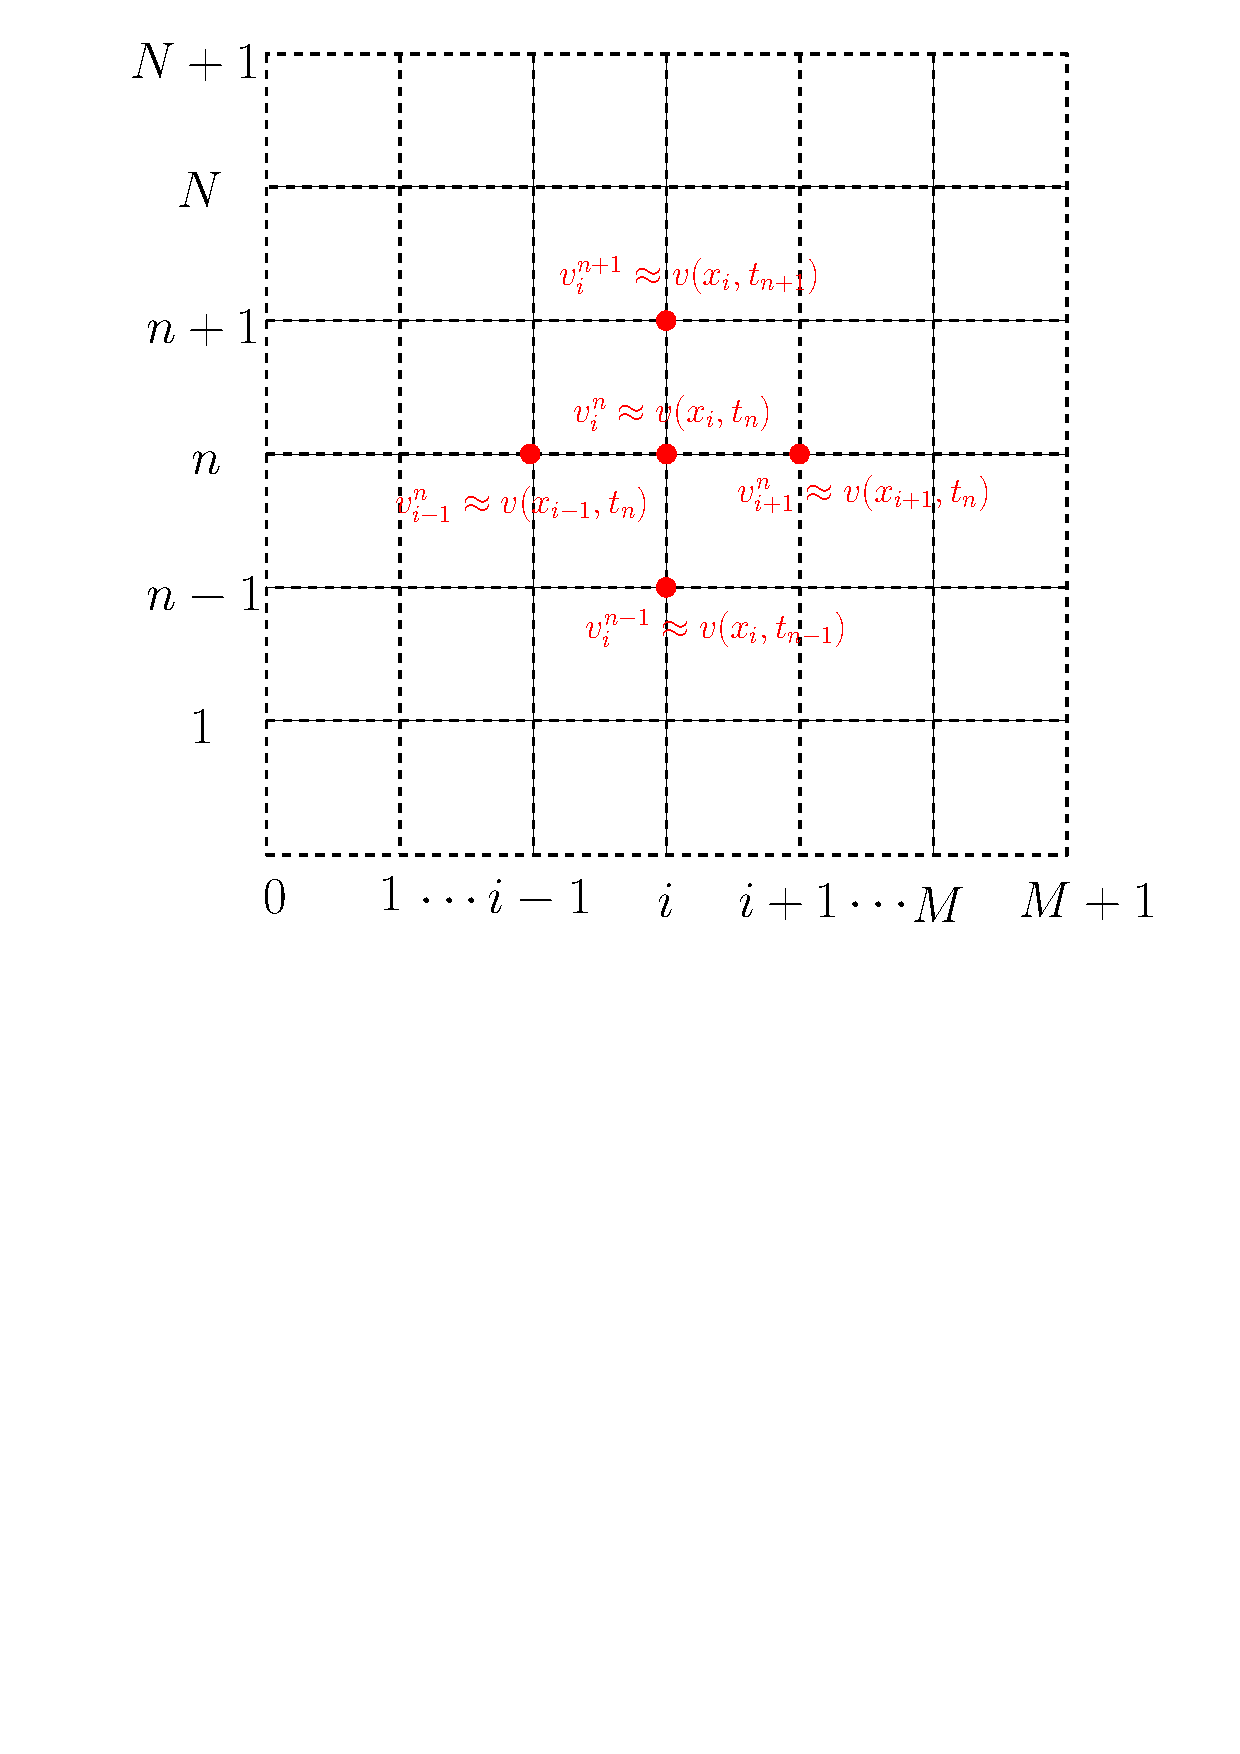
\includegraphics[scale=0.5]{chapters/chapter3/GridAproximation.pdf}
  \caption{The grid $\mathcal{G}$ and the approximation $v^{n}_{i} \approx v(x_i, t_n)$ in each node.}
\end{figure}
From \eqref{eq:finitedifferencesschemes:overview:continous_domain}, it is clear that $t_\text{min} = 0$ and $t_\text{max}=T$. Moreover, for call options, $x_\text{min} = 0$ and $x_\text{max}=1$. Likewise, for put options, $x_\text{min}=1$ and $x_\text{max}=x_\infty$ where $x_\infty$ is arbitrary large value.
Now that we defined our grid, our goal is to approximate the value function $v(x, t)$ and the optimal exercise price $\bar{S}(t)$ at each node of the grid $\mathcal{G}$
\begin{align*}
  v^{n}_i \approx v(x_i,t_n), \quad \bar{S}^{n} \approx \bar{S}(t_n)
\end{align*}
Moreover, we want that the error of the approximation converges to zero value. Specifically, we want that the approximation error at each node 
\begin{align}
  \label{eq:finitedifferencesschemes:overview:local_truncation_error}
  e^{n}_i := v^{n}_i-v(x_i, t_n)
\end{align}
goes to zero as $\Delta{x}$ and $\Delta{t}$ decrease. \eqref{eq:finitedifferencesschemes:overview:local_truncation_error} is the local truncation error, and it measures the approximation error at time $t_n$. It is important to state if a single node has inferior order than the rest of the nodes, it might degrade the order of the truncation error in overall.   

Finally, we need ways to approximate derivatives. Here is where finite differences schemes come into play. The idea of finite differences is trivial which is approximating derivatives as the difference of contiguous nodes in the grid. Let us say we are at point $x$, then the forward differences approximate the derivative as
\begin{align*}
 \dfrac{f(x + h) - f(x)}{h} = \dfrac{df}{dx} + O(h)
\end{align*}
Conversely, the backward difference approximate the derivative as 
\begin{align*}
  \dfrac{f(x) - f(x-h)}{h} = \dfrac{df}{dx} + O(h)
\end{align*}
As you can observe forward and backward difference approximation yield a local truncation error of $O(h)$. Moreover, the central finite difference approximate the first order derivative as 
\begin{align*}
  \dfrac{f(x+h) - f(x-h)}{2h} = \dfrac{df}{dx} + O(h^2)
 \end{align*}
and for second order derivatives as
\begin{align*}
  \dfrac{f(x+h) - 2f(x) + f(x-h)}{h^2} = \dfrac{d^2f}{dx^2} + O(h^2)
 \end{align*}
Note that both approximation offers a better order of convergence that forward and backward difference, but you are required to come up with strategies for approximating the derivative at the boundary of your grid where $x+h$ or $x-h$ is not defined.

\subsection{Explicit scheme}
Generally, explicit schemes use forward finite difference to approximate the temporal partial derivative and central finite difference to approximate the spatial derivative at time $t_{n+1}$ and position $x_i$. However, since the problem \eqref{eq:blackscholes:frontfixingmethod:inversetransform:american_options_bs_pde} is written backward in time, we use backward finite difference at $t_{n+1}$, and a central finite difference at $x_i$.

\begin{figure}[H]
  \centering
  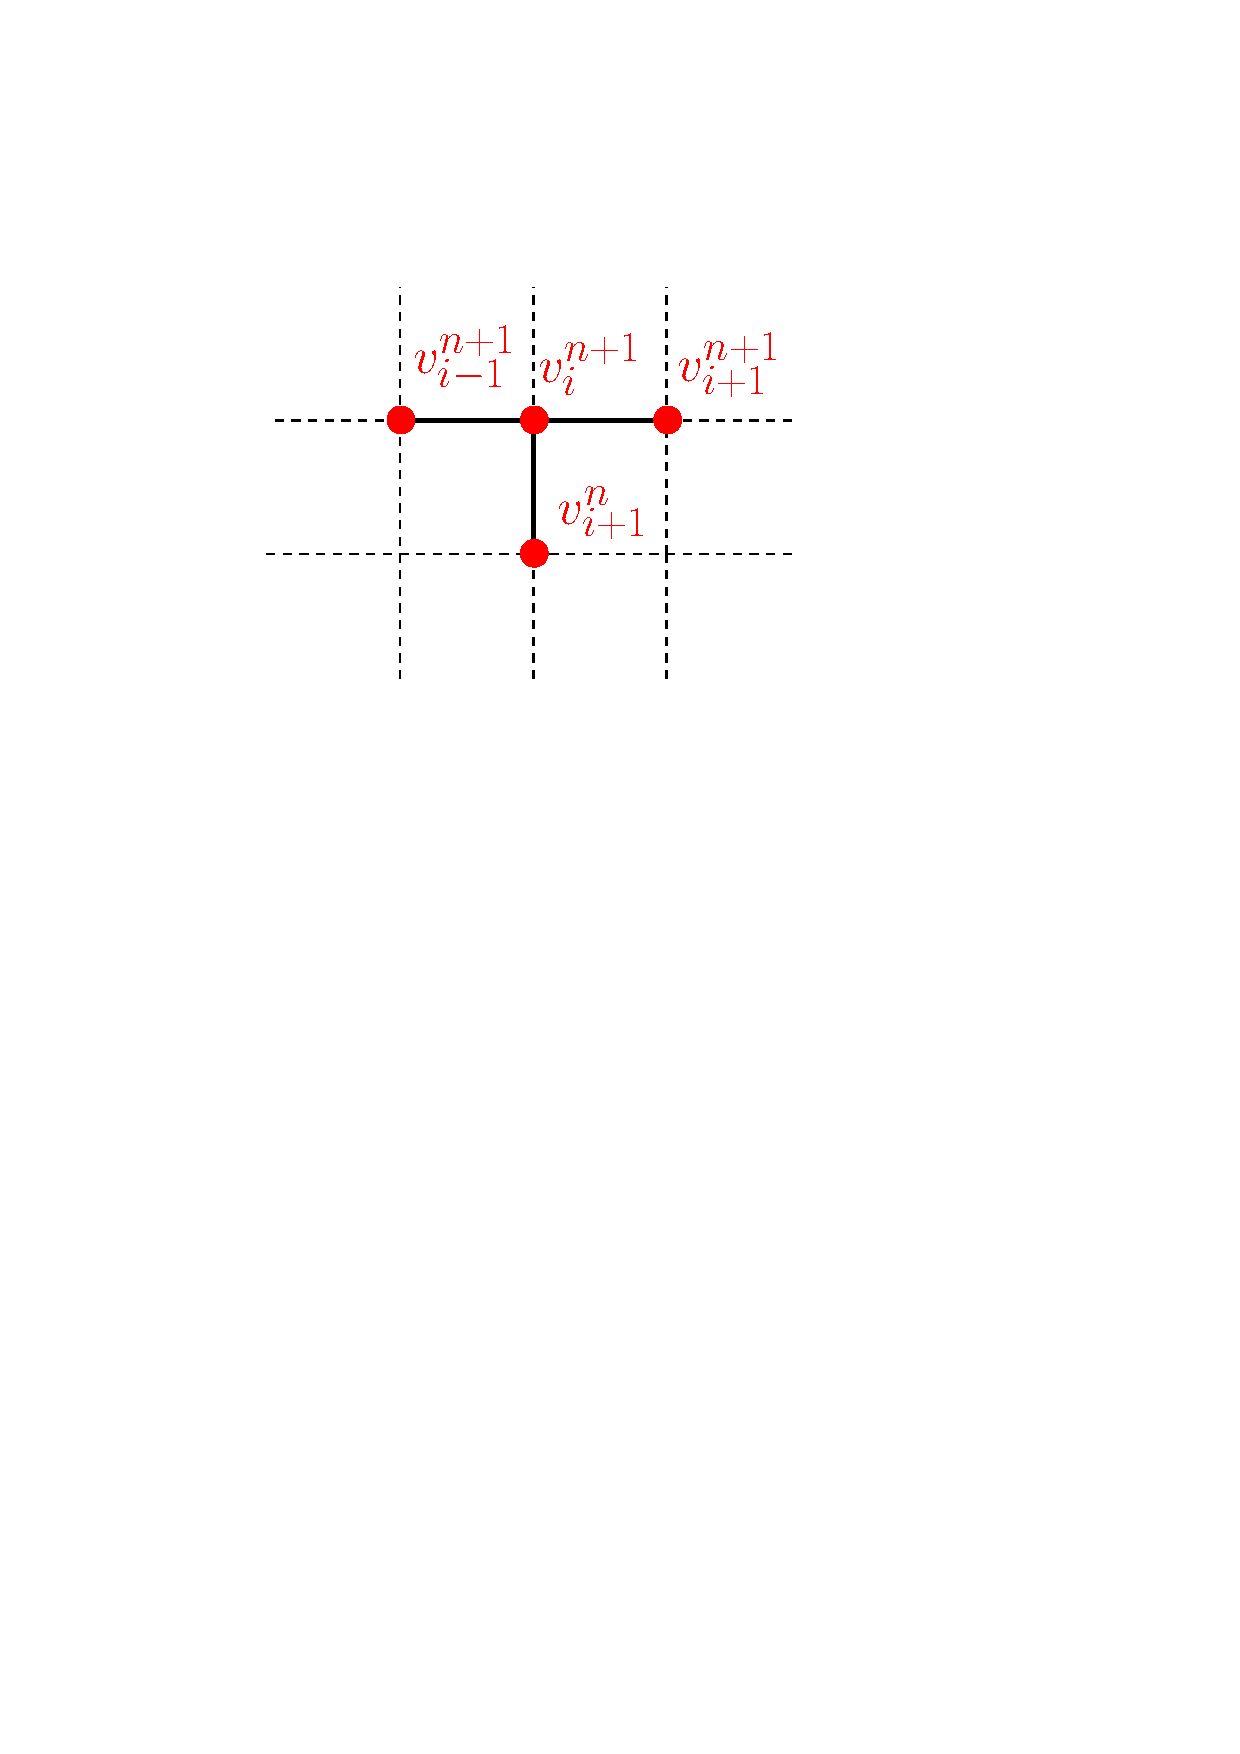
\includegraphics[scale=.8]{chapters/chapter3/ExplicitStencil.pdf}
  \caption{Stencil diagram of the explicit scheme.}
  \label{fig:finitedifferencesschemes:explicit_stencil}
\end{figure}

The central finite difference for the first order and second order spatial partial derivative is given by
\begin{align}
  \label{eq:finitedifferencesschemes:explicit:spatial_first_order_central_finite_difference}
  \dfrac{v^{n+1}_{i+1} - v^{n+1}_{i-1}}{2 \Delta{x}} =& \dfrac{\partial{v}}{\partial{x}}+ O(\Delta{x}^2) \qquad & \text{for $i = 1, \dots, M$} \\
  \label{eq:finitedifferencesschemes:explicit:spatial_second_order_central_finite_difference}
  \dfrac{v^{n+1}_{i+1} - 2v^{n+1}_{i} + v^{n+1}_{i-1}}{\Delta{x}^2} =& \dfrac{\partial^2{v}}{\partial{x^2}}+ O(\Delta{x}^2) \qquad & \text{for $i = 1, \dots, M$}
\end{align}
As it can be observed in figure \eqref{fig:finitedifferencesschemes:explicit_stencil}, the first and second order central finite difference approximations at node $(x_i, t_{n+1})$ require to compute the difference at the nodes $(x_{i-1}, t_{n+1})$ and $(x_{i+1}, t_{n+1})$. Hence, we can only approximate the spatial partial derivative at the internal region of the grid $\mathcal{G}$ given by the nodes $(x_i, t_n)$ for $i=1,\dots,M$. Also note, that the central finite difference has second order convergence in space. In other words, as we decrease $\Delta{x}$ by one decimal place, the approximation error will decrease by two decimal places.

Analogously, the backward difference approximation at $t_{n+1}$ for $v(x, t)$ and the optimal exercise price $\bar{S}(t)$ is given by
\begin{align}
  \label{eq:finitedifferencesschemes:explicit:temporal_backward_finite_difference}
  \dfrac{v^{n+1}_{i} - v^{n}_{i}}{\Delta{t}} &= \dfrac{\partial{v}}{\partial{t}}+ O(\Delta{t}) \qquad & \text{for $n = N,\dots,0$ } \\
  \label{eq:finitedifferencesschemes:explicit:front_temporal_backward_finite_difference}
  \dfrac{\bar{S}^{n+1}-\bar{S}^{n}}{\Delta t} &= \bar{S}'(t) + O(\Delta{t}) \qquad & \text{for $n = N,\dots,0$ }
\end{align}
Contrary to the central finite difference, the backward finite difference approximations have first order convergence in time. While it would be desirable to have second order convergence for the temporal partial derivative approximation, it is not possible use central finite difference because we would be required to have two boundary conditions in the time axis. By combining the finite difference approximations \eqref{eq:finitedifferencesschemes:explicit:spatial_first_order_central_finite_difference}, \eqref{eq:finitedifferencesschemes:explicit:spatial_second_order_central_finite_difference}, \eqref{eq:finitedifferencesschemes:explicit:temporal_backward_finite_difference}, and \eqref{eq:finitedifferencesschemes:explicit:temporal_backward_finite_difference},the approximation of the PDE in \eqref{eq:blackscholes:frontfixingmethod:inversetransform:american_options_bs_pde} is given by 
\begin{equation*}
  \begin{split}
    \dfrac{v^{n+1}_{i} - v^{n}_{i}}{\Delta{t}} & + \dfrac{1}{2}\sigma^2 x_i^2 \dfrac{v^{n+1}_{i-1} - 2v^{n+1}_{i} + v^{n+1}_{i+1}}{(\Delta{x})^2} \\ 
     & + x_i\bigg( (r-\delta) - \dfrac{1}{\bar{S}^{n+1}}\dfrac{\bar{S}^{n+1} - \bar{S}^{n}}{\Delta{t}} \bigg)\dfrac{v^{n+1}_{i+1} - v^{n+1}_{i-1}}{2\Delta{x}} - rv^{n+1}_{i} = 0
  \end{split}
\end{equation*}
for $i = 1, \dots, M$ and $n = N, \dots, 0$. To simplify the expression above, we introduce the terms 
\begin{align*}
  \lambda &:= \dfrac{\Delta{t}}{(\Delta{x})^2} \\
  A_i &:= \dfrac{\lambda}{2}\sigma^2x^{2}_i - \dfrac{\lambda}{2}\bigg((r-\delta) - \dfrac{1}{\Delta{t}}\bigg)x_i\Delta{x} & \text{for $i = 1, \dots, M$} \\ 
  B_i &:= 1 - \lambda\sigma^2x_i^2 - r\Delta{t} & \text{for $i = 1, \dots, M$} \\
  C_i &:= \dfrac{\lambda}{2}\sigma^2x^{2}_i + \dfrac{\lambda}{2}\bigg((r-\delta) - \dfrac{1}{\Delta{t}}\bigg)x_i\Delta{x} &  \text{for $i = 1, \dots, M$} \\
  D^{n+1}_{i} &:= \dfrac{x_i}{2\Delta{x}}\dfrac{v^{n+1}_{i+1} - v^{n+1}_{i-1}}{\bar{S}^{n+1}} &  \text{for $i = 1, \dots, M$}
\end{align*}
Then, we rearrange the finite difference approximation of the PDE as 
\begin{equation}
  v^{n}_{i} - D^{n+1}_{i}\bar{S}^n = A_i v^{n+1}_{i-1} + B_{i}v^{n+1}_{i} + C_{i}v^{n+1}_{i+1}
  \label{eq:finitedifferencesschemes:explicit:pde_simplified}
\end{equation}
for $i = 1, \dots, M$ and $t = N, \dots, 0$. Moreover, the PDE problem in \eqref{eq:blackscholes:frontfixingmethod:inversetransform:american_options_bs_pde} have well-defined spatial boundary conditions. For call options, the boundary conditions are located at $x=0$ and $x=1$. Similarly, for put options, the boundary conditions are located at $x=1$ and at a sufficient large $x$. However, since the $\mathcal{G}$ is defined in terms of $x_\text{min}$ and $x_\text{max}$, regardless of the option type, the boundary conditions will be always at $x_0$ and $x_{M+1}$.
\begin{subequations}
  \label{eq:finitedifferencesschemes:explicit:boundary_conditions}
  \begin{align}
    \text{\textbf{Call:}} \qquad & v^{n}_{0} = 0, \qquad v^{n}_{M+1} = \bar{S}^{n} - K\\
    \text{\textbf{Put:}} \qquad & v^{n}_{0} = K - \bar{S}^{n}, \qquad v^{n}_{M+1} = 0
  \end{align}
\end{subequations}
Likewise, the terminal conditions are located at $t_{N+1}$ $i=0,\dots,M+1$
\begin{subequations}
  \label{eq:finitedifferencesschemes:explicit:terminal_conditions}
  \begin{equation}
    v^{N+1}_{i} = 0, \qquad \bar{S}^{N+1} = K
  \end{equation}
\end{subequations}
Moreover, for the problem \eqref{eq:blackscholes:frontfixingmethod:inversetransform:american_options_bs_pde}, we have contact point condition \eqref{eq:blackscholes:frontfixingmethod:inversetransform:american_options_optimal_price_contact_point_condition}. The contact point condition gives the slope at $x=1$. When the option is a call option, $x=1$ correspond to $x_{M+1}$ in the grid $\mathcal{G}$. Reciprocally, for a put option, $x=1$ correspond to $x_0$. Therefore, by using backward difference at $x_{M+1}$ and forward difference at $x_0$, the contact point approximation for call and put options, respectively.
\begin{align*}
  \text{\textbf{Call:}} \qquad & \dfrac{v^{n}_{M+1} - v^{n}_{M}}{\Delta{x}} = \dfrac{\partial{v}}{\partial{x}}(1, t) + O(\Delta{x}) \\
  \text{\textbf{Put:}} \qquad & \dfrac{v^{n}_{1} - v^{n}_{0}}{\Delta{x}} = \dfrac{\partial{v}}{\partial{x}}(1, t)+ O(\Delta{x}) 
\end{align*}
Using the contact point condition, we obtain an explicit expression for $v^{n}_{M}$
\begin{subequations}
  \label{eq:finitedifferencesschemes:explicit:contact_point_approximation_2}
  \begin{align}
    \text{\textbf{Call:}} \qquad& v^{n}_{M} = v^{n}_{M+1} - \Delta{x}\bar{S}^{n} = (1-\Delta{x})\bar{S}^n - K & \qquad \text{for $n = N,\dots,0$ }\\
    \text{\textbf{Put:}} \qquad& v^{n}_{1} = v^{n}_{0} - \Delta{x}\bar{S}^{n} = K - (1+\Delta{x})\bar{S}^n & \qquad \text{for $n = N,\dots,0$ }
  \end{align}    
\end{subequations}
Note that the approximation for $v^{n}_{M}$ has first order convergence in space which could degrade the global convergence of the explicit method to first order in space even if we are using central finite difference to approximate the spatial partial derivatives of $v(x,t)$. Similarly, we can obtain explicit expression for $\bar{S}^{n}$ by computing \eqref{eq:finitedifferencesschemes:explicit:pde_simplified} at $x_M$ and at $x_1$ for call and put options, respectively. Then, rearranging the resulting expression in terms of $\bar{S}^n$ 
\begin{subequations}
  \label{eq:finitedifferencesschemes:explicit:optimal_exercise_price_approximation}
  \begin{align}
    \text{\textbf{Call:}} \qquad& \bar{S}^{n} = \dfrac{K + A_{M}v^{n+1}_{M-1} + B_{M}v^{n+1}_{M} + C_{M}v^{n+1}_{M+1}}{(1-\Delta{x}) - D^{n+1}_{M}} \\
    \text{\textbf{Put:}} \qquad& \bar{S}^{n} = \dfrac{K - (A_{1}v^{n+1}_{0} + B_{1}v^{n+1}_{1} + C_{1}v^{n+1}_{2})}{D^{n+1}_1 + (1+\Delta{x})}
  \end{align}
\end{subequations}
for $n = N,\dots,0$. Thus, combining \eqref{eq:finitedifferencesschemes:explicit:pde_simplified}, \eqref{eq:finitedifferencesschemes:explicit:boundary_conditions}, 
\eqref{eq:finitedifferencesschemes:explicit:terminal_conditions},
\eqref{eq:finitedifferencesschemes:explicit:contact_point_approximation_2}, and \eqref{eq:finitedifferencesschemes:explicit:optimal_exercise_price_approximation}, the explicit scheme of PDE problem \eqref{eq:blackscholes:frontfixingmethod:inversetransform:american_options_bs_pde} is given by
\begin{subequations}
  \label{eq:finitedifferencesschemes:explicit:nielsen_system_of_equation}
  \begin{align}
    \text{\textbf{Call:}} \quad& \begin{cases}
      v^{n}_{i} - D^{n+1}_{i}\bar{S}^n = A_i v^{n+1}_{i-1} + B_{i}v^{n+1}_{i} + C_{i}v^{n+1}_{i+1} & \text{for $i = 1, \dots, M-1$ and $n = N,\dots, 0$}\\
      v^{N+1}_i = 0 & \text{for $i = 0, \dots, M+1$}  \\
      \bar{S}^{N+1} = K \\
      v^{n}_0 = 0 & \text{for $n = N, \dots, 0$} \\ 
      v^{n}_{M} = (1-\Delta{x})\bar{S}^n - K & \text{for $n = N, \dots, 0$} \\
      v^{n}_{M+1} = \bar{S}^n - K  & \text{for $n = N, \dots, 0$}
    \end{cases}\\
    \text{\textbf{Put:}} \quad&  \begin{cases}
      v^{n}_{i} - D^{n+1}_{i}\bar{S}^n = A_i v^{n+1}_{i-1} + B_{i}v^{n+1}_{i} + C_{i}v^{n+1}_{i+1} & \text{for $i = 2, \dots, M$ and $n = N,\dots,0$} \\
      v^{N+1}_i = 0 & \text{for $i = 0, \dots, M+1$} \\ 
      \bar{S}^{N+1} = K \\
      v^{n}_{0} = K - \bar{S}^{n} & \text{for $n = N, \dots, 0$} \\
      v^{n}_{1} =  K - (1+\Delta{x})\bar{S}^{n}  & \text{for $n = N, \dots, 0$} \\
      v^{n}_{M} = 0 & \text{for $n = N, \dots 0$}
    \end{cases}
  \end{align}
\end{subequations}
Finally, we formulate an algorithm for solving the system \eqref{eq:finitedifferencesschemes:explicit:nielsen_system_of_equation}
\begin{algorithm}[H]
  \caption{Explicit method for call options} \label{alg:finitedifferencesschemes:explicit:call_explicit_method_algorithm}
  \begin{algorithmic}
  \Ensure $\lambda \le 0.5$
  
  \For{$i = 0,\dots,M+1$} 
    \State $v^{N+1}_i = 0 $
  \EndFor
  
  \State $\bar{S}^{N+1} = K$

  \For{$i = 1,\dots,M$} 
    \State $A_i = \dfrac{\lambda}{2}\sigma^2x^{2}_i - \dfrac{\lambda}{2}\bigg((r-\delta) - \dfrac{1}{\Delta{t}}\bigg)x_i\Delta{x}$
    \State $B_i = 1 - \lambda\sigma^2x_i^2 - r\Delta{t} $
    \State $C_i = \dfrac{\lambda}{2}\sigma^2x^{2}_i + \dfrac{\lambda}{2}\bigg((r-\delta) - \dfrac{1}{\Delta{t}}\bigg)x_i\Delta{x} $
  \EndFor
  
  \For{$n = N, \dots, 0$}
    \For{$i = 1, \dots, M$}
      \State $D^{n+1}_i = \dfrac{x_i}{2\Delta{x}}\dfrac{v^{n+1}_{i+1} - v^{n+1}_{i-1}}{\bar{S}^{n+1}}$
    \EndFor
    \State $\bar{S}^n = \dfrac{K + A_{M}v^{n+1}_{M-1} + B_{M}v^{n+1}_{M} + C_{M}v^{n+1}_{M+1}}{(1-\Delta{x}) - D^{n+1}_{M}}$
    \State $v^{n}_{0} = 0$
    \State $v^{n}_{M} = (1-\Delta{x})\bar{S}^{n} - K$
    \State $v^{n}_{M+1} = \bar{S}^{n} - K$
    \For{$i = 1, \dots, M-1$}
      \State $v^{n}_{i} = A_i v^{n+1}_{i-1} + B_{i}v^{n+1}_{i} + C_{i}v^{n+1}_{i+1} + D^{n+1}_{i}\bar{S}^n$
    \EndFor
  \EndFor
\end{algorithmic}
\end{algorithm}

\begin{algorithm}[H]
  \caption{Explicit method for put options}\label{alg:finitedifferencesschemes:explicit:put_explicit_method_algorithm}
  \begin{algorithmic}
  \For{$i = 0,\dots,M+1$} 
    \State $v^{N+1}_i = 0 $
  \EndFor
  \State $\bar{S}^{N+1} = K$
  \For{$i = 1,\dots,M$} 
    \State $A_i = \dfrac{\lambda}{2}\sigma^2x^{2}_i - \dfrac{\lambda}{2}\bigg((r-\delta) - \dfrac{1}{\Delta{t}}\bigg)x_i\Delta{x}$
    \State $B_i = 1 - \lambda\sigma^2x_i^2 - r\Delta{t} $
    \State $C_i = \dfrac{\lambda}{2}\sigma^2x^{2}_i + \dfrac{\lambda}{2}\bigg((r-\delta) - \dfrac{1}{\Delta{t}}\bigg)x_i\Delta{x} $
  \EndFor
  \For{$n = N, \dots, 0$}
    \For{$i = 1, \dots, M$}
      \State $D^{n+1}_i = \dfrac{x_i}{2\Delta{x}}\dfrac{v^{n+1}_{i+1} - v^{n+1}_{i-1}}{\bar{S}^{n+1}}$
    \EndFor
    \State $\bar{S}^n = \dfrac{K - (A_{1}v^{n+1}_{0} + B_{1}v^{n+1}_{1} + C_{1}v^{n+1}_{2})}{D^{n+1}_{1} + (1+\Delta{x})}$
    \State $v^{n}_{0} = K - \bar{S}^{n}$
    \State $v^{n}_{1} = K - (1+\Delta{x})\bar{S}^n$
    \State $v^{n}_{M+1} = 0$
    \For{$i = 2, \dots, M$}
      \State $v^{n}_{i} = A_i v^{n+1}_{i-1} + B_{i}v^{n+1}_{i} + C_{i}v^{n+1}_{i+1} + D^{n+1}_{i}\bar{S}^n$
    \EndFor
  \EndFor
\end{algorithmic}
\end{algorithm}
\newpage
\subsection{Implicit scheme}
Analogously to the previous section, implicit methods approximate the temporal partial derivative using backward difference and the spatial partial derivative using a central difference at time $t_n$ and position $x_i$. Since the PDE in \eqref{eq:blackscholes:frontfixingmethod:inversetransform:american_options_bs_pde} is written backward in time, we use a forward difference instead.
\begin{figure}[H]
  \centering
  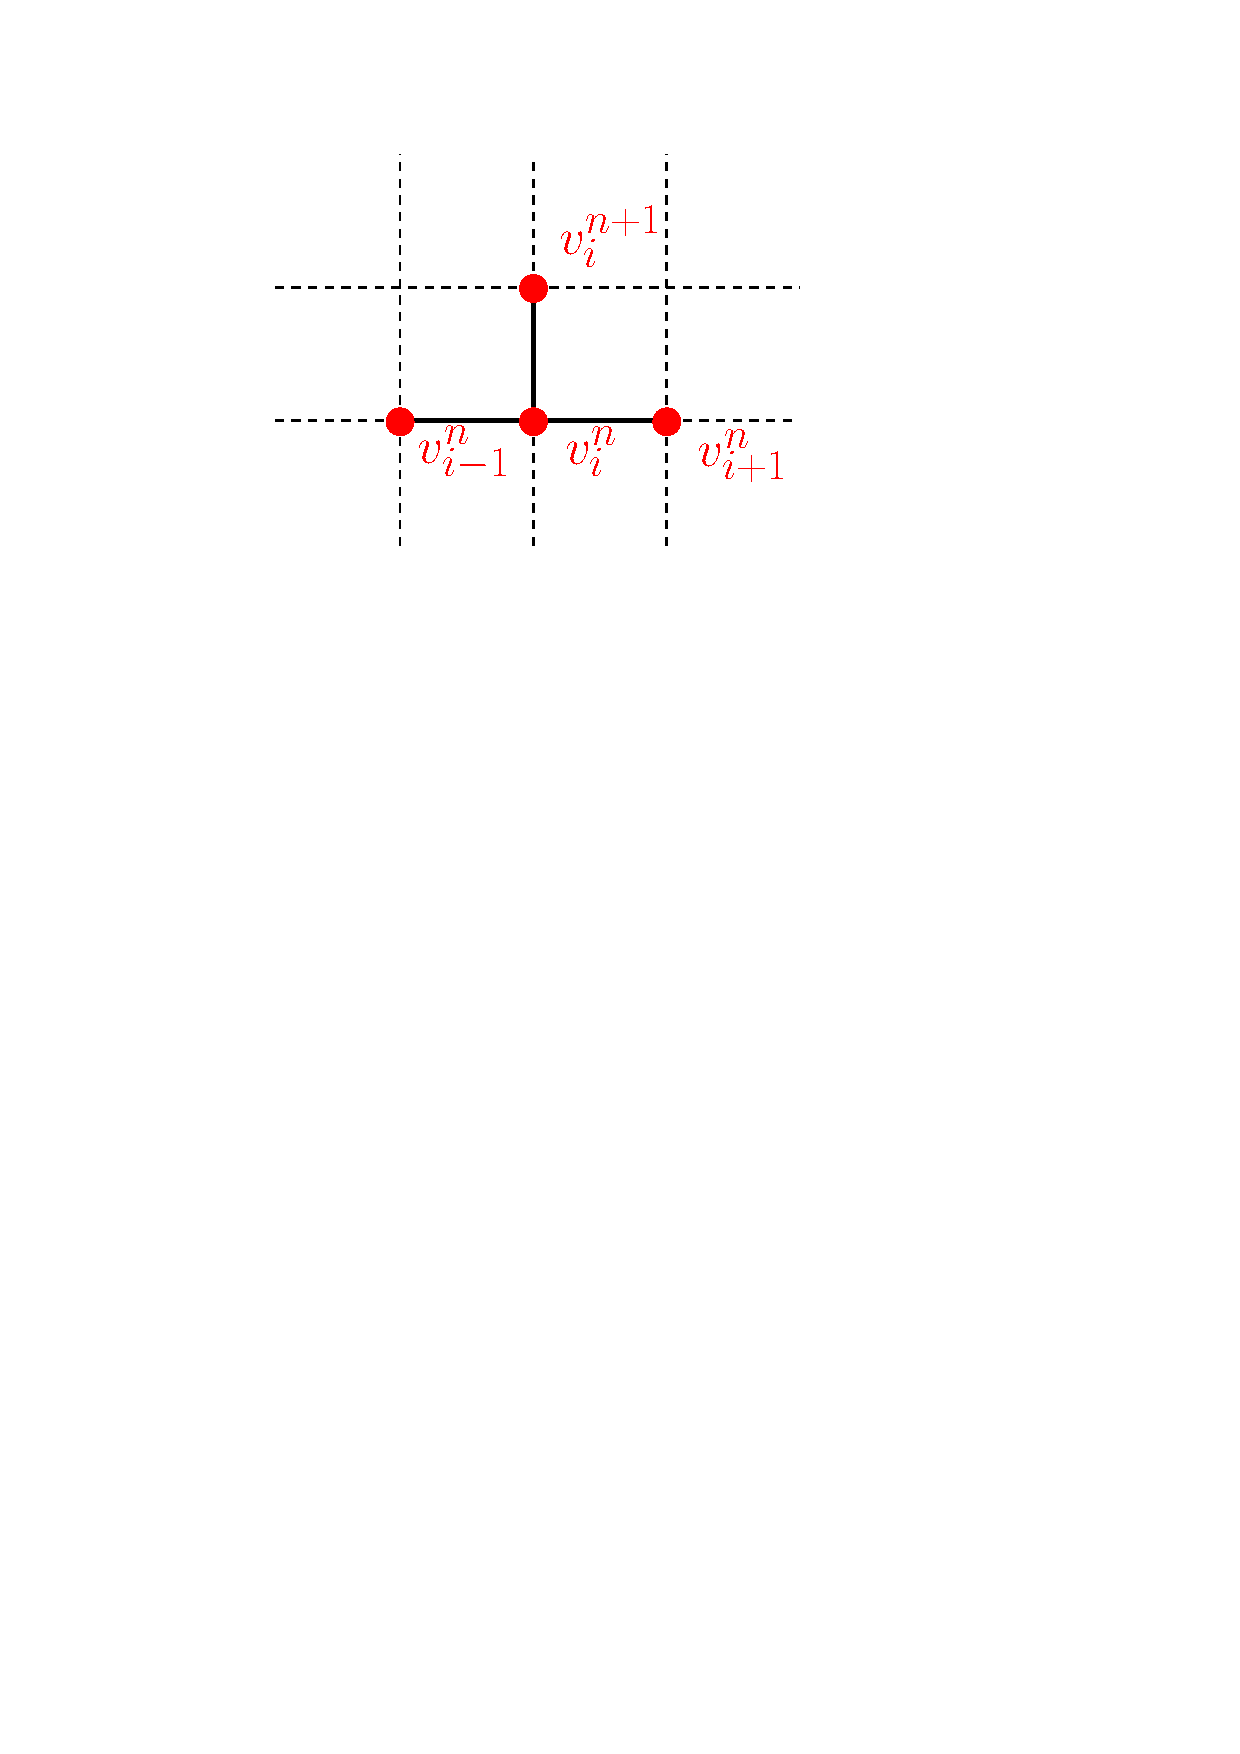
\includegraphics[scale=.8]{chapters/chapter3/ImplicitStencil.pdf}
  \caption{Stencil diagram of the implicit scheme.}
  \label{fig:finitedifferencesschemes:implicit_stencil}
\end{figure}
Therefore, the central difference for the first and second order spatial partial derivative at time $t_n$ is 
\begin{align}
  \label{eq:finitedifferencesschemes:implicit:spatial_first_order_central_finite_difference}
  \dfrac{v^{n}_{i+1} - v^{n}_{i-1}}{2 \Delta{x}} =& \dfrac{\partial{v}}{\partial{x}}+ O(\Delta{x}^2) \\
  \label{eq:finitedifferencesschemes:implicit:spatial_second_order_central_finite_difference}
  \dfrac{v^{n}_{i+1} - 2v^{n}_{i} + v^{n}_{i-1}}{\Delta{x}^2} =& \dfrac{\partial^2{v}}{\partial{x^2}}+ O(\Delta{x}^2)
\end{align}
for $i = 1, \dots, M$. Likewise, the forward difference of $v(x, t)$ and $\bar{S}(t)$ at position $x_i$ is  
\begin{align}
  \label{eq:finitedifferencesschemes:implicit:temporal_backward_finite_difference}
  \dfrac{v^{n+1}_{i} - v^{n}_{i}}{\Delta{t}} &= \dfrac{\partial{v}}{\partial{t}}+ O(\Delta{t}) \\
  \label{eq:finitedifferencesschemes:implicit:front_temporal_backward_finite_difference}
  \dfrac{\bar{S}^{n+1}-\bar{S}^{n}}{\Delta t} &= \bar{S}'(t) + O(\Delta{t}) \qquad & \text{ }
\end{align}
for $n = N,\dots,0$. Hence, combining \eqref{eq:finitedifferencesschemes:implicit:spatial_first_order_central_finite_difference}, \eqref{eq:finitedifferencesschemes:implicit:spatial_second_order_central_finite_difference}, \eqref{eq:finitedifferencesschemes:implicit:temporal_backward_finite_difference} and \eqref{eq:finitedifferencesschemes:implicit:front_temporal_backward_finite_difference},we obtain the implicit approximation of the PDE \eqref{eq:blackscholes:frontfixingmethod:inversetransform:american_options_bs_pde} as
\begin{equation*}
  \begin{split}
    \dfrac{v^{n+1}_{i} - v^{n}_{i}}{\Delta{t}} & + \dfrac{1}{2}\sigma^2 x_i^2 \dfrac{v^{n}_{i-1} - 2v^{n}_{i} + v^{n}_{i+1}}{(\Delta{x})^2} \\ 
     & + x_i\bigg( (r-\delta) - \dfrac{1}{\bar{S}^{n}}\dfrac{\bar{S}^{n+1} - \bar{S}^{n}}{\Delta{t}} \bigg)\dfrac{v^{n}_{i+1} - v^{n}_{i-1}}{2\Delta{x}} - rv^{n}_{i} = 0
  \end{split}
\end{equation*}
for $i=1,\dots,M$ and $n=N,\dots,0$. Similar to the explicit method, the approximation error is second order in space and first order in time. Again, to make the implicit  approximation more manageable, we introduce the following terms  
\begin{align}
  \alpha^{n}_{i} &:= -\dfrac{\lambda}{2}\sigma^2x^{2}_{i} + \dfrac{\lambda\Delta{x}}{2}x_{i}\bigg(r-\delta+\dfrac{\bar{S}^{n+1}-\bar{S}^n}{\Delta{t}\bar{S}^{n}}\bigg) \\
  \beta^{n}_{i} &:= 1 + \lambda\sigma^2x^{2}_{i} + r\Delta{t} \\
  \gamma^{n}_{i} &:= -\dfrac{\lambda}{2}\sigma^2x^{2}_{i} + \dfrac{\lambda\Delta{x}}{2}x_{i}\bigg(r-\delta+\dfrac{\bar{S}^{n+1}-\bar{S}^n}{\Delta{t}\bar{S}^{n}}\bigg)
\end{align}
and rearrange the PDE as
\begin{equation}
  \label{eq:finitedifferencesschemes:implicit:implicit_scheme_simplified}
  \alpha^{n}_{i}v^{n}_{i-1} + \beta^{n}_{i}v^{n}_{i} + \gamma^{n}_{i}v^{n}_{i+1} = v^{n+1}_{i}
\end{equation}
The boundary and terminal conditions are given by \eqref{eq:finitedifferencesschemes:explicit:boundary_conditions} and \eqref{eq:finitedifferencesschemes:explicit:terminal_conditions}. Likewise, the approximation of $v^{n}_{M}$ or $v^{n}_{1}$ for put and call, respectively, is given by \eqref{eq:finitedifferencesschemes:explicit:contact_point_approximation_2}. Similar to the explicit method, the approximation $v^{n}_{M}$ and $v^{n}_{0}$ given by the contact point condition is first order in space. Hence, the global approximation error of implicit scheme might be degraded to first order in space. Contrary to the explicit method, there is not an explicit expression for $\bar{S^n}$. Now, we formulate the system of equations of the problem \eqref{eq:blackscholes:frontfixingmethod:inversetransform:american_options_bs_pde}
using \eqref{eq:finitedifferencesschemes:explicit:boundary_conditions}, \eqref{eq:finitedifferencesschemes:explicit:terminal_conditions}, \eqref{eq:finitedifferencesschemes:explicit:contact_point_approximation_2} and \eqref{eq:finitedifferencesschemes:implicit:implicit_scheme_simplified}
\begin{subequations}
  \label{eq:finitedifferencesschemes:implicit:nielsen_system_of_equation}
  \begin{align}
    \text{\textbf{Call:}} \quad& \begin{cases}
      \alpha^{n}_{i}v^{n}_{i-1} + \beta^{n}_{i}v^{n}_{i} + \gamma^{n}_{i}v^{n}_{i+1} = v^{n+1}_{i} & \text{for $i = 1, \dots, M-1$ and $n = N,\dots,0$} \\
      v^{N+1}_i = 0 & \text{for $i = 0, \dots, M+1$}\\
      \bar{S}^{N+1} = K \\
      v^{n}_0 = 0 & \text{for $n = N, \dots 0$}\\
      v^{n}_{M} = (1-\Delta{x})\bar{S}^n - K & \text{for $n = N, \dots 0$}\\
      v^{n}_{M+1} = \bar{S}^n - K  & \text{for $n = N, \dots 0$}
    \end{cases}\\
    \text{\textbf{Put:}} \quad& \begin{cases}
      \alpha^{n}_{i}v^{n}_{i-1} + \beta^{n}_{i}v^{n}_{i} + \gamma^{n}_{i}v^{n}_{i+1} = v^{n+1}_{i} & \text{for $i = 2, \dots, M$ and $n = N,\dots,0$} \\
      v^{N+1}_i = 0 & \text{for $i = 0, \dots, M+1$} \\
      \bar{S}^{N+1} = K \\
      v^{n}_{0} = K - \bar{S}^{n} & \text{for $n = N, \dots 0$}\\
      v^{n}_{1} =  K - (1+\Delta{x})\bar{S}^{n} & \text{for $n = N, \dots 0$}\\
      v^{n}_{M} = 0 & \text{for $n = N, \dots 0$}
    \end{cases}
  \end{align}
\end{subequations}
Since there is not an explicit formula for $v^{n}_{i}$ and $\bar{S}^n$, we will 
have to solve a non-linear system of equation. Let's define the vector $\mathbf{v}^n \in \mathbb{R}^{M-1}$ 
\begin{subequations}
  \begin{align}
    \text{\textbf{Call:}} \qquad \mathbf{v}^{n} :=& \begin{bmatrix}
      v^{n}_{1}, & v^{n}_{2}, & \cdots, & v^{n}_{M-1}
    \end{bmatrix}^{\text{T}}\\
    \text{\textbf{Put:}} \qquad \mathbf{v}^{n} :=& \begin{bmatrix}
      v^{n}_{2}, & v^{n}_{3}, & \cdots, & v^{n}_{M}
    \end{bmatrix}^{\text{T}}
  \end{align}    
\end{subequations}
the matrix $\Lambda^{n} \in \mathbb{R}^{M-1,M-2}$ 
\begin{subequations}
  \begin{align}
    \text{\textbf{Call:}} \qquad \Lambda^{n} =& \begin{bmatrix}
      \beta^{n}_{1} & \gamma^{n}_1 \\
      \alpha^{n}_{2} & \beta^{n}_{2} & \gamma^{n}_{2} \\
      & \ddots & \ddots & \ddots  \\
      & & \ddots & \ddots & \ddots  \\
      & & & \alpha^{n}_{M-2} & \beta^{n}_{M-2} & \gamma^{n}_{M-2} \\
      & & & & \alpha^{n}_{M-1} & \beta^{n}_{M-1} \\
      & & & & & \alpha^{n}_{M} \\
    \end{bmatrix}\\
    \text{\textbf{Put:}} \qquad  \Lambda^{n} :=& \begin{bmatrix}
      \gamma^{n}_1 \\
      \beta^{n}_2 & \gamma^{n}_2 \\
      \alpha^{n}_3 & \beta^{n}_3 & \gamma^{n}_3 \\
      & \ddots & \ddots & \ddots \\
      & & \ddots & \ddots & \ddots \\
      & & & \alpha^{n}_{M-1} & \beta^{n}_{M-1} & \gamma^{n}_{M-1} \\
      & & & & \alpha^{n}_{M} & \beta^{n}_{M} \\
    \end{bmatrix}
  \end{align}
\end{subequations}
and the vector $\mathbf{f}^{n} \in \mathbb{R}^{M-1}$
\begin{subequations}
  \begin{align}
    \text{\textbf{Call:}} \qquad \mathbf{f}^n :=& \begin{bmatrix}
      v^{n+1}_{1} \\
      \vdots \\
      v^{n+1}_{M-1} - \gamma^{n}_{M-1}[(1-\Delta{x})\bar{S}^{n} - K] \\
      v^{n+1}_{M} - \gamma^{n}_{M}(\bar{S}^n - K) - \beta^{n}_{M}[(1-\Delta{x})\bar{S}^{n} - K]
    \end{bmatrix}\\
    \text{\textbf{Put:}} \qquad \mathbf{f}^n :=& \begin{bmatrix}
      v^{n+1}_{1} - \alpha^{n}_{1}(K - \bar{S}^{n}) - \beta^{n}_{1}[K - (1+\Delta{x})\bar{S}^{n}] \\
      v^{n+1}_{2} - \beta^{n}_2[K - (1+\Delta{x})\bar{S}^{n}] \\
      v^{n+1}_{3} \\
      \vdots \\
      v^{n+1}_{M-1}
    \end{bmatrix}
  \end{align}
\end{subequations}
Thus, the non-linear system of equations that we need to solve is
\begin{equation}
  F(\mathbf{v}^{n}, \bar{S}^{n}) = \Lambda^{n}\mathbf{v}^{n} - \mathbf{f}^n = 0
\end{equation}

By computing the Jacobian of the system, we con solve the non-linear system 
using the newton's method

\begin{equation}
  \mathbf{y}_{k+1} = \mathbf{y}_{k} - J^{-1}(\mathbf{y}_{k})F(\mathbf{y}_{k})
\end{equation}

where $y_k$ is some approximation of the solution
\begin{equation}
  \mathbf{y} = \begin{bmatrix}
    \mathbf{v}^{n} | \bar{S}^{n}
  \end{bmatrix}^{\text{T}}
\end{equation}

\subsection{Numerical results}
Generally, Datasets for American options are hard to get and often require paying substantial amount of money. Therefore, to validate our implementation, we mainly relied on the data available in Company, 
et al. \cite*{company_egorova_jodar_2014}, Nielsen, et al. \cite*{nielsen_2001}, Seydel \cite*{seydel_2009}, and Wilmott, et al. \cite*{wilmott_howison_dewynne_1995}. Moreover, we used the approximations produced by the binomial model introduced by Cox et al. \cite{cox_1979} as benchmark for assessing the consistency of our method. We chose the binomial model because it uses a completely different approach to price options than the one considered in our work, is widely used in the industry, and is simple to implement. First, 
we want to assess the correct functionality of our implementation. Naturally, the first test that come into main is to price call and put options without dividend. Therefore, we define the set of parameters taken from \cite{nielsen_2001}

\begin{equation}
  \label{eq:numericaresults:parameters_set_1}
  K = 1, \quad T = 1, \quad r=0.2, \quad \sigma=0.02, \quad \delta = 0 
\end{equation}

Additionally, We use Nielsen \cite{nielsen_2001} optimal exercise boundary $\bar{S}(t) \approx 0.86$ for parameters as a reference \eqref{eq:numericaresults:parameters_set_1}. Also, we approximated $\bar{S}(t)$ using the binomial option pricing model also as a reference. Finally, we priced call and put options using our implementation of the explicit \eqref{eq:finitedifferencesschemes:explicit:nielsen_system_of_equation} and implicit \eqref{eq:finitedifferencesschemes:implicit:nielsen_system_of_equation} method for the Nielsen transformation, and the explicit method for the Company transformation \eqref{alg:appendix:companytransformation:explicits:put_explicit_method_algorithm} (See appendix). As you can observe in figure \eqref{fig:finitedifferencesschemes:numericaresults:test_case_1_explicit_company},
\eqref{fig:finitedifferencesschemes:numericaresults:test_case_1_explicit_nielsen}, and \eqref{fig:finitedifferencesschemes:numericaresults:test_case_1_implicit_nielsen},
our implementation for the Nielsen and Company transformation seems to produce the value as per \eqref{fig:blackscholes:preliminaries:american_call_value_vs_curve}. However, by taking a look to figure \eqref{fig:finitedifferencesschemes:numericaresults:test_case_1_bopm}, you can observe that the binomial option pricing model is also not capturing the geometrical properties defined in figure \eqref{fig:blackscholes:preliminaries:american_call_value_vs_curve}. This behavior can explain by saying that American call options without dividends cannot be modelled using \eqref{eq:blackscholes:preliminaries:call_american_options_pde_free_boundary_problem_full}. In fact, Merton \cite{merton_1973} showed that, pricing American options without dividends is equivalent to solve \eqref{eq:chapter2:european_option_pde_with_dividens}. Therefore, we can conclude that we applied the wrong methods to price call options without dividends. 
\begin{figure}[tbp]
  \centering
  \begin{subfigure}{0.4\textwidth}
    \centering
    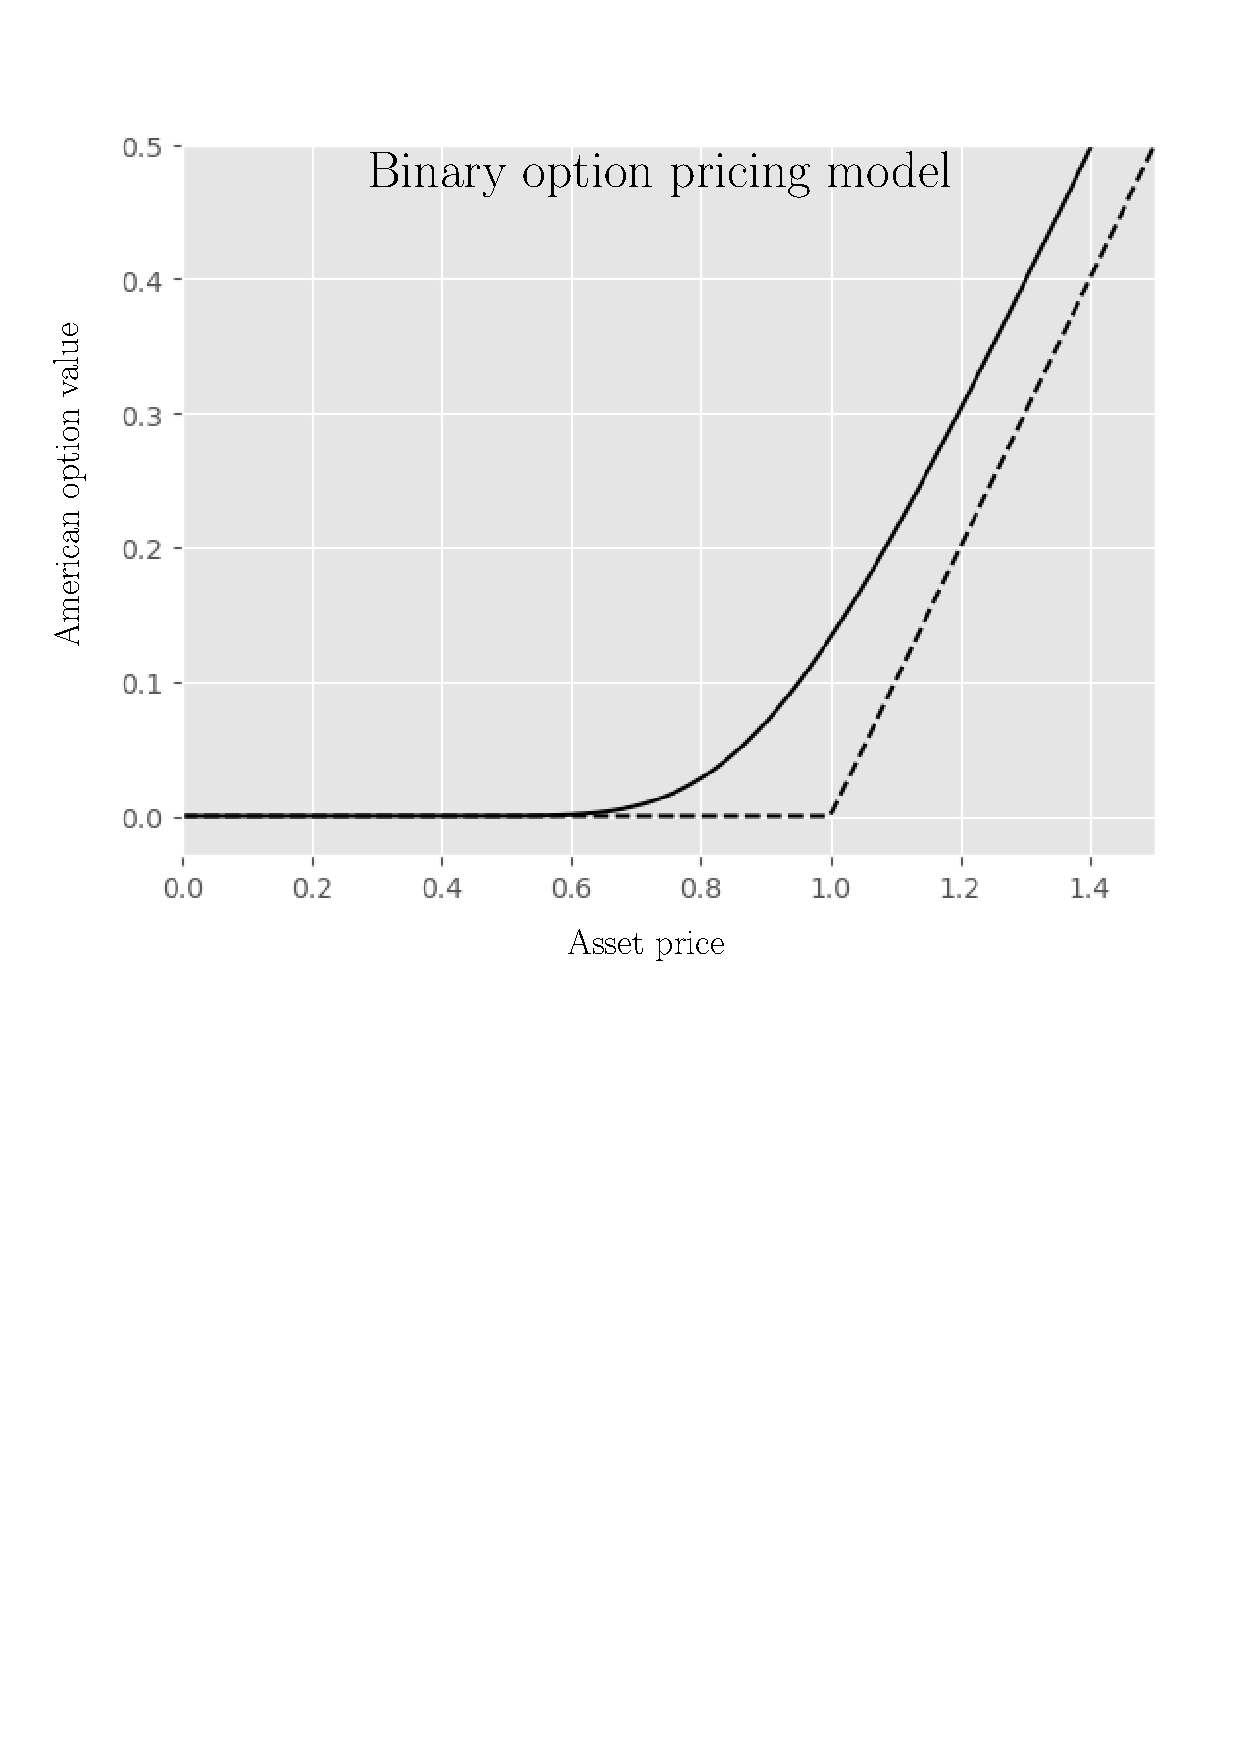
\includegraphics[width=\textwidth]{chapters/chapter3/TestCase1BOPM.pdf}
    \caption{$\text{Nodes} = 2^{500}$.}
    \label{fig:finitedifferencesschemes:numericaresults:test_case_1_bopm}
  \end{subfigure}
  \hspace{0.5cm}
  \begin{subfigure}{0.4\textwidth}
    \centering
    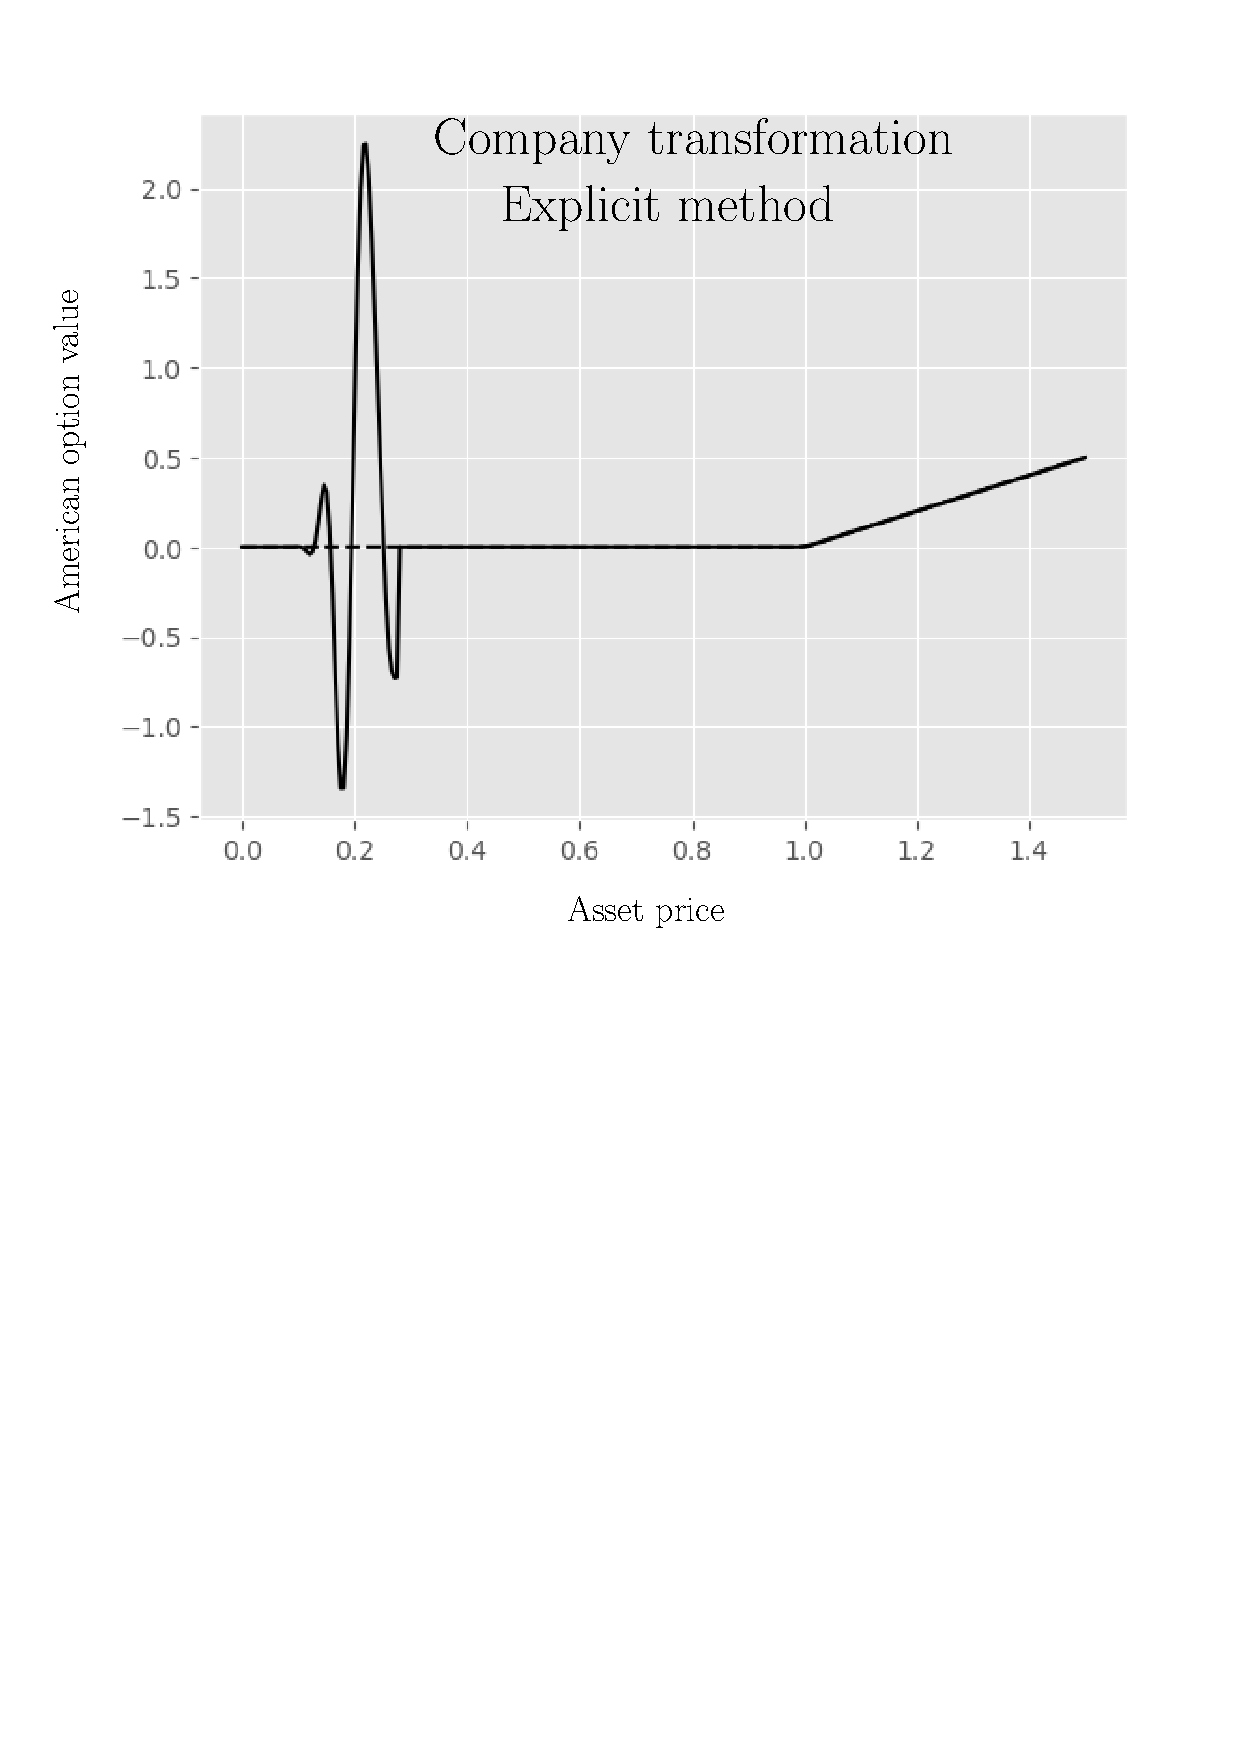
\includegraphics[width=\textwidth]{chapters/chapter3/TestCase1ExplicitCompany.pdf}
    \caption{$\Delta{x}=\expnumber{1}{-3}$ and $\Delta{t}=0.5\times\expnumber{1}{-6}$}
    \label{fig:finitedifferencesschemes:numericaresults:test_case_1_explicit_company}
  \end{subfigure}
  \begin{subfigure}{0.4\textwidth}
    \centering
    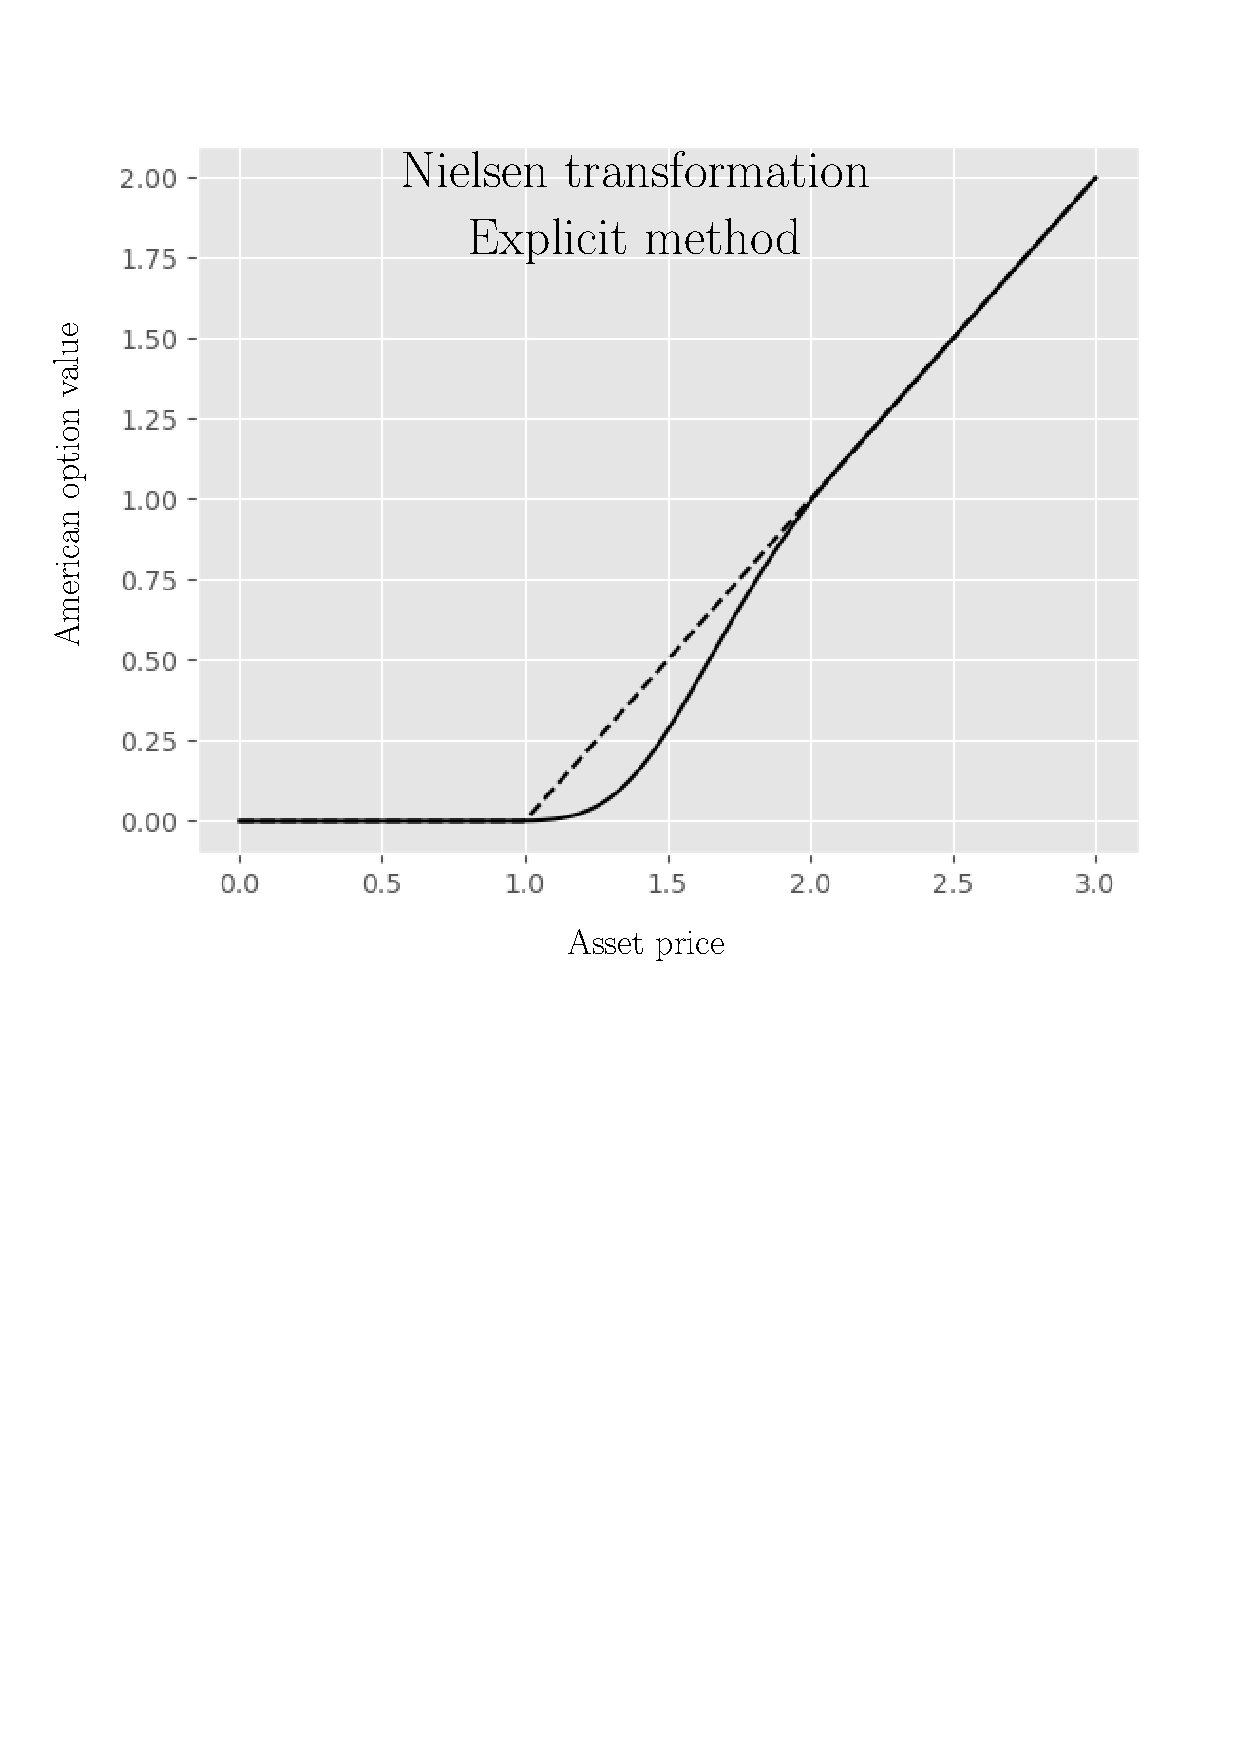
\includegraphics[width=\textwidth]{chapters/chapter3/TestCase1ExplicitNielsen.pdf}
    \caption{$\Delta{x}=\expnumber{1}{-3}, \Delta{t}=0.5\times\expnumber{1}{-6}$}
    \label{fig:finitedifferencesschemes:numericaresults:test_case_1_explicit_nielsen}
  \end{subfigure}
  \hspace{0.5cm}
  \begin{subfigure}{0.4\textwidth}
    \centering
    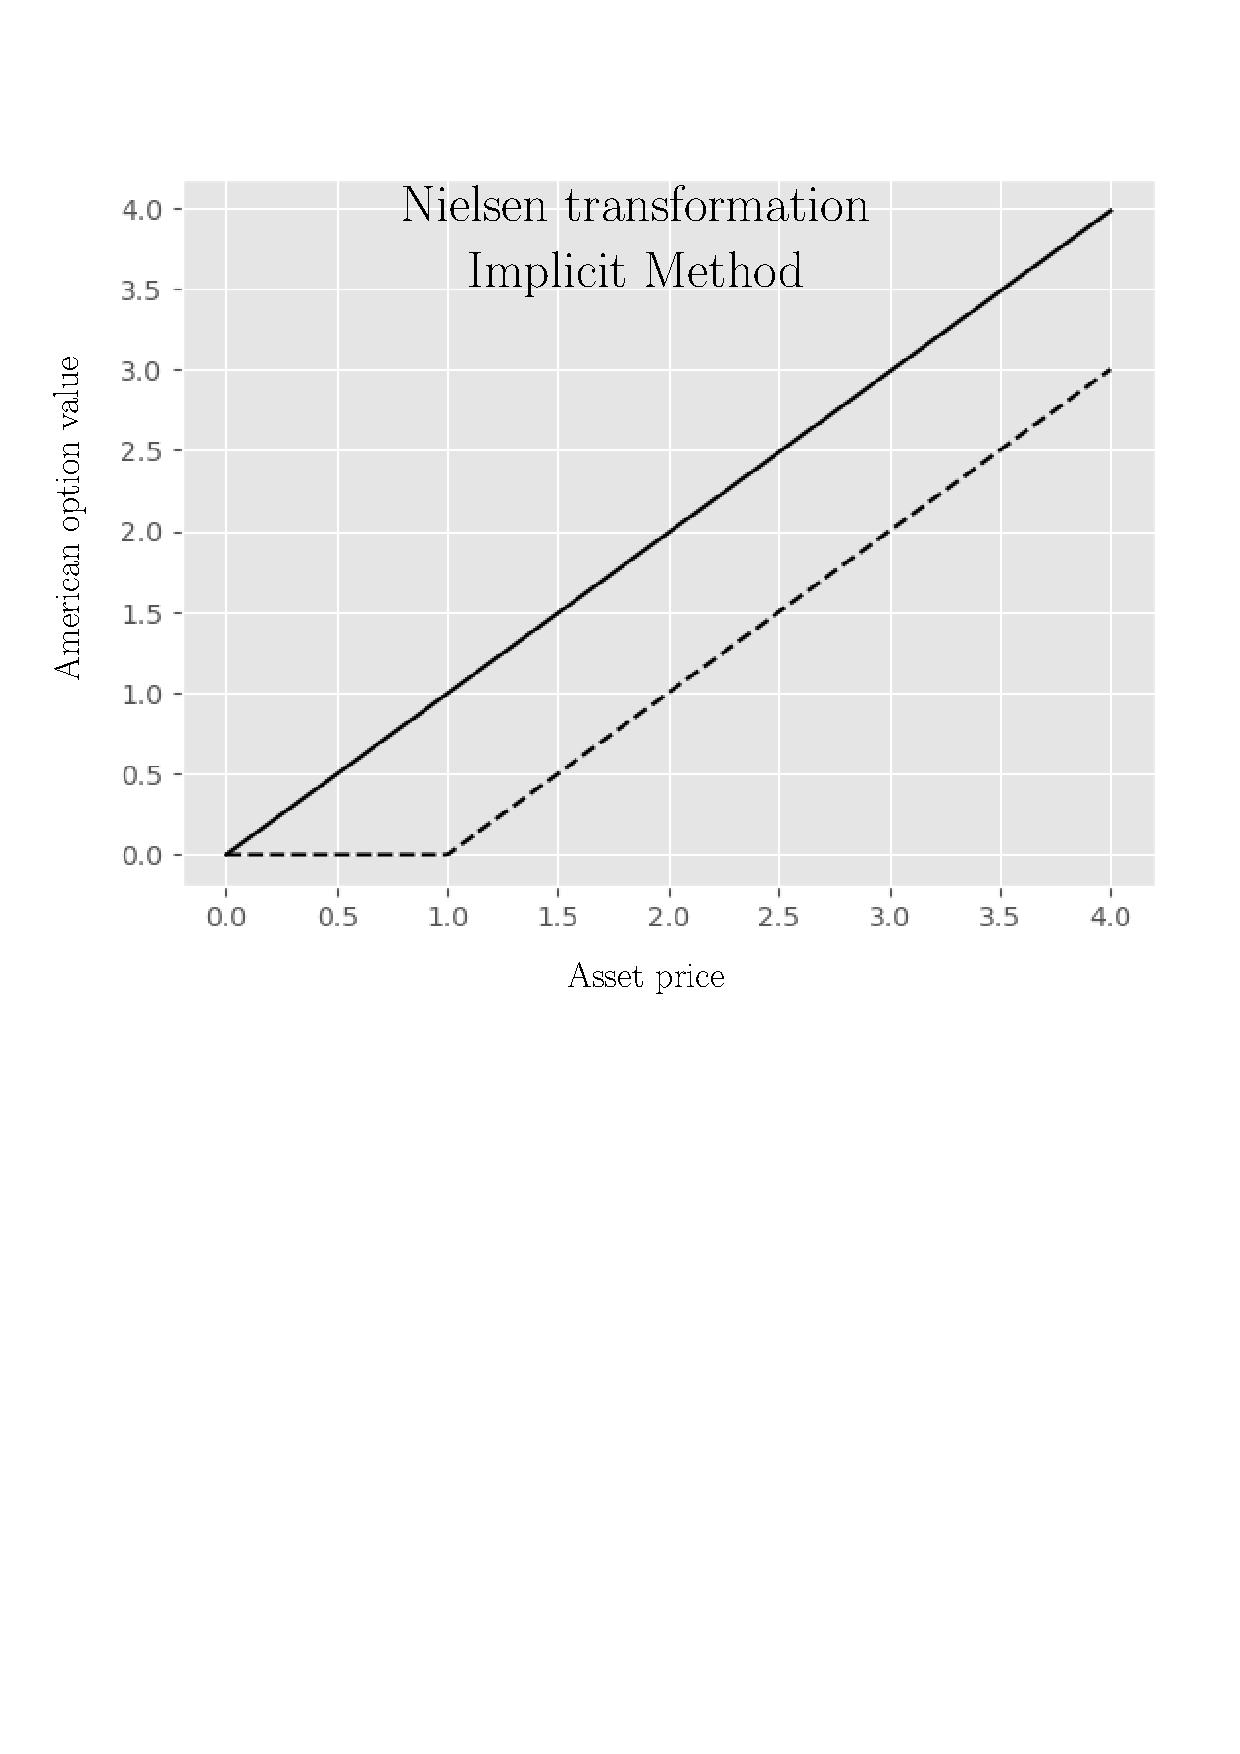
\includegraphics[width=\textwidth]{chapters/chapter3/TestCase1ImplicitNielsen.pdf}
    \caption{$\Delta{x}=\expnumber{1}{-3}, \Delta{t}=0.5\times\expnumber{1}{-6}$}
    \label{fig:finitedifferencesschemes:numericaresults:test_case_1_implicit_nielsen}
  \end{subfigure}
  \caption{American call option value $V(S, 0)$ curve.}
  \label{fig:finitedifferencesschemes:numericaresults:test_case_1_explicit}
\end{figure}

Now, let us consider the case for put options without dividends for the same given parameters. Figures \eqref{fig:finitedifferencesschemes:numericaresults:test_case_2} show the $V(S, 0)$ curve obtained by the Nielsen and Company explicit method. In each plot, we have listed the optimal exercise boundary $\bar{S}(0)$. Also, we have listed the correspondent value curve produced using the binary option pricing model using $2^{500}$ nodes. As you see, Nielsen and Company approximated the optimal exercise boundary within 2 decimal places. Moreover, in table \eqref{tab:rsme_explicit_company_transformation}, you can find the RMSE error produced by the explicit method for the Company transformation. Other tables can be found in appendix \eqref{sec:numericalexperiments}.  Contrary to the case for call options, you can observe in figures \eqref{fig:finitedifferencesschemes:numericaresults:test_case_2} that the approximations of the value curve $V(S,t)$ captures the geometry of American put options described by figure \eqref{fig:blackscholes:preliminaries:american_put_value_vs_curve}. Specifically, within the continuation region $S>\bar{S}(0)$, the value is larger than the payoff function and as S gets larger, the value goes to zero. In addition, the value curve is exactly the payoff. Also notice that the RSME of the explicit method for the Company transformation fairly low which indicate us that our implementation for the method works for American put options.

\begin{figure}[tbp]
  \centering
  \begin{subfigure}{0.4\textwidth}
    \centering
    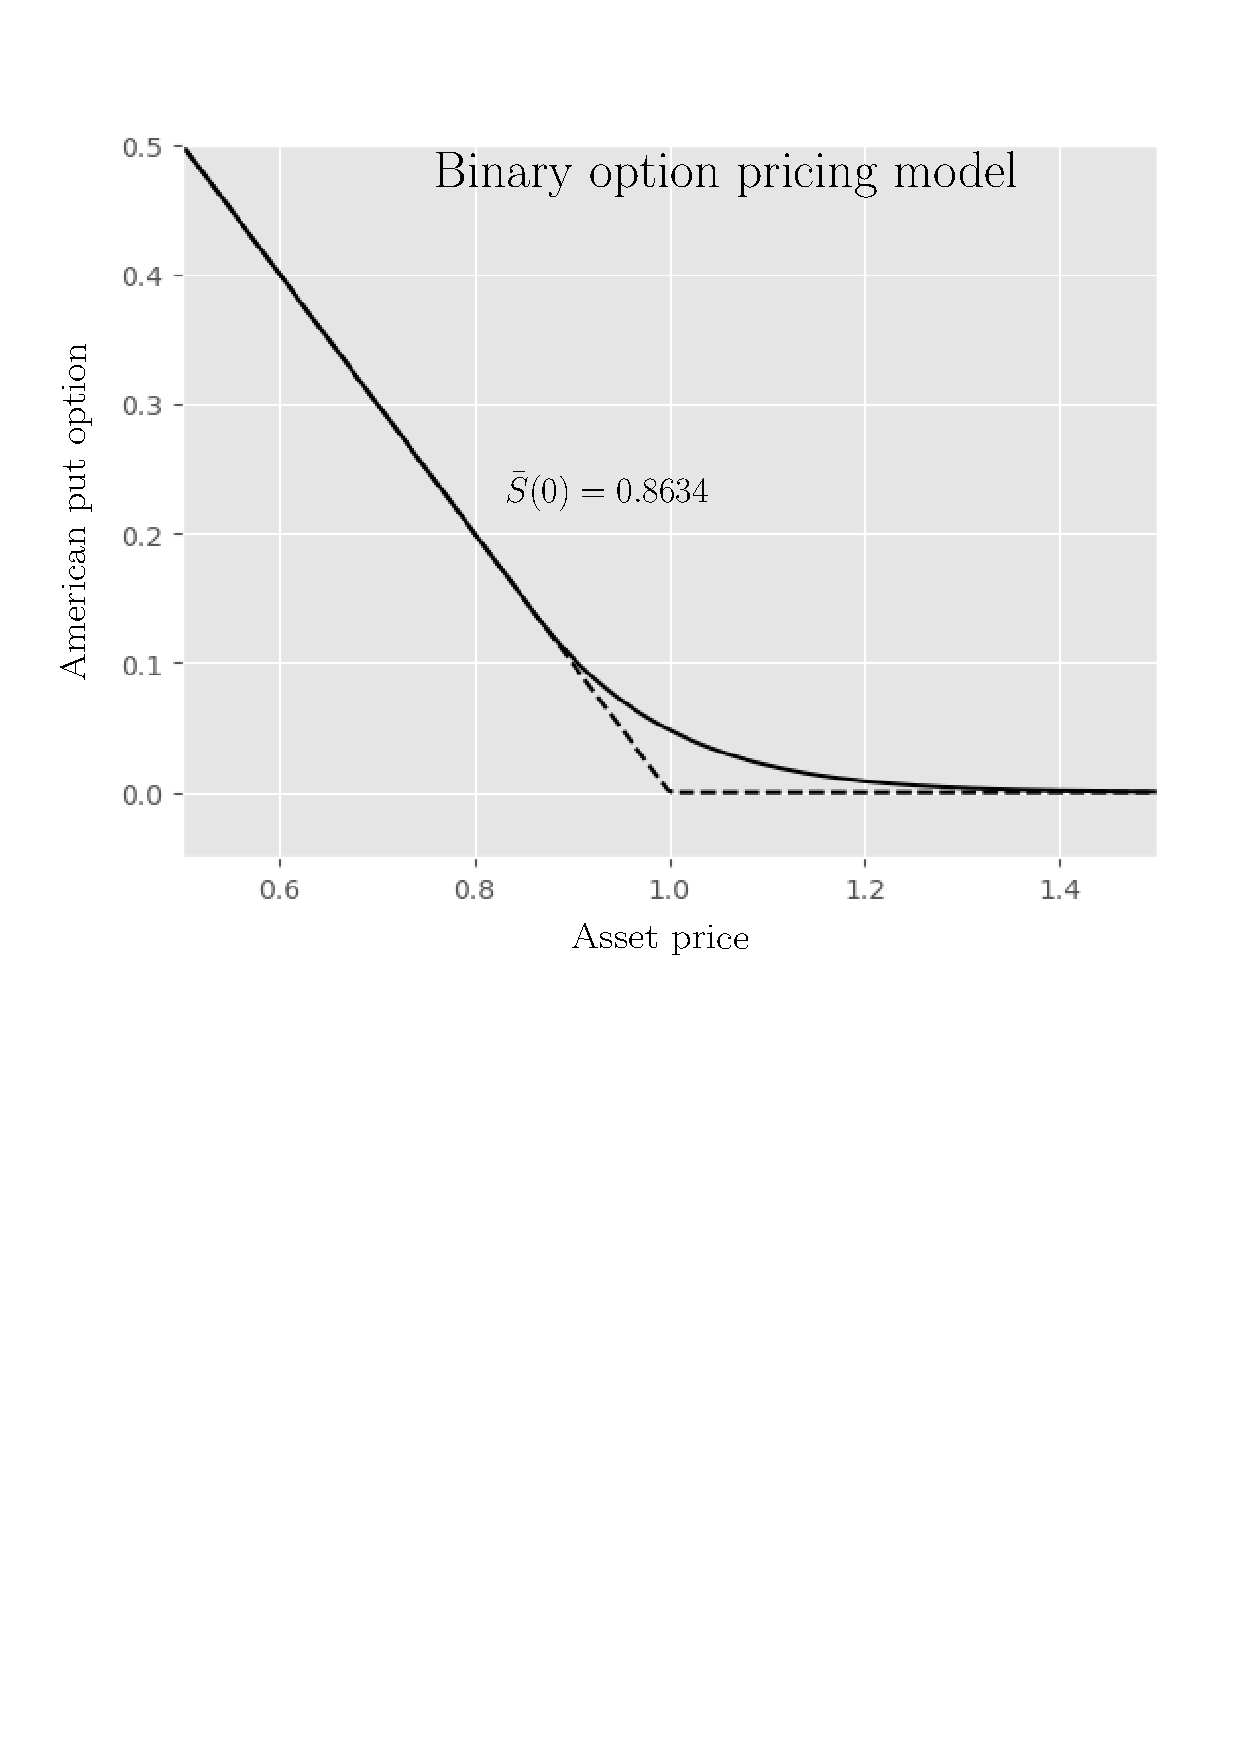
\includegraphics[width=\textwidth]{chapters/chapter3/TestCase2BOPM.pdf}
    \caption{$\text{Nodes} = 2^{500}$.}
    \label{fig:finitedifferencesschemes:numericaresults:test_case_2_bopm}
  \end{subfigure}
  \hspace{0.5cm}
  \begin{subfigure}{0.4\textwidth}
    \centering
    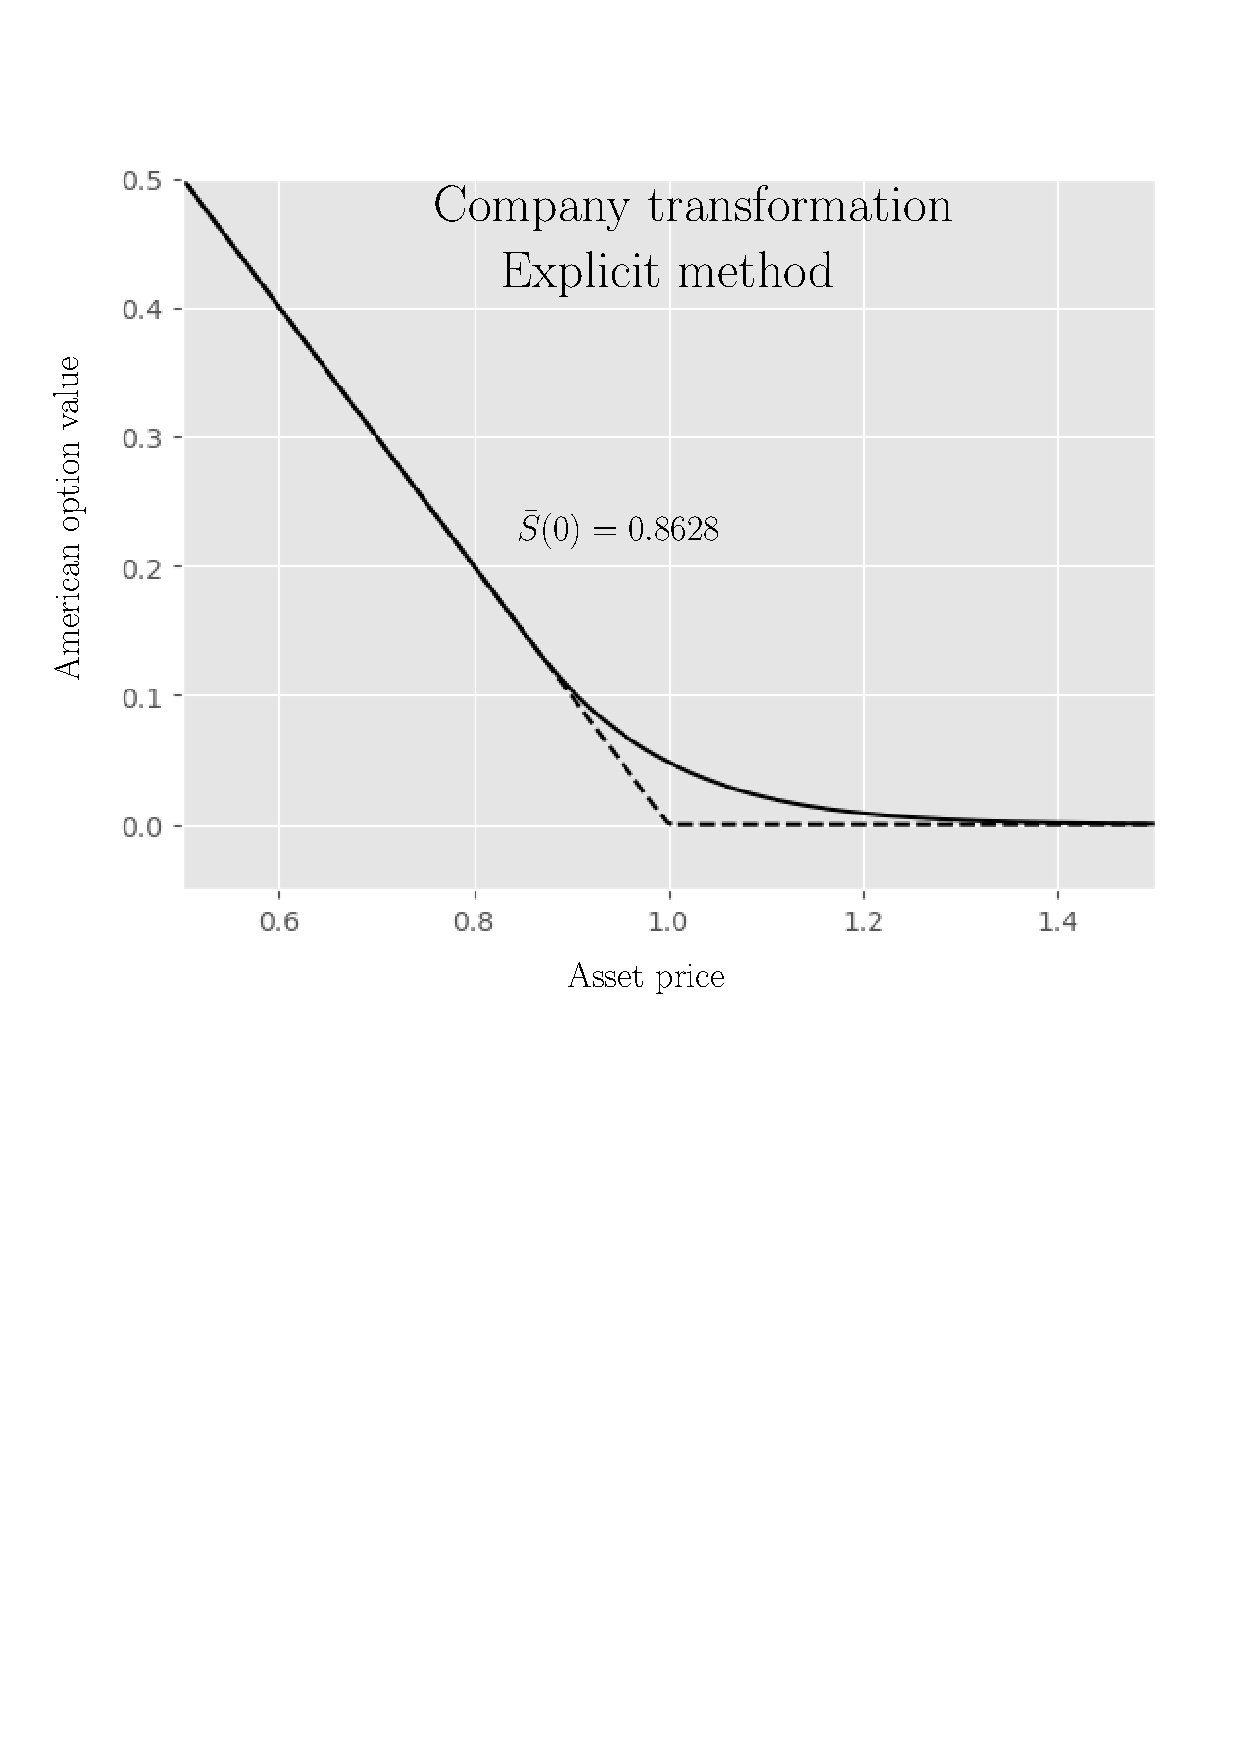
\includegraphics[width=\textwidth]{chapters/chapter3/TestCase2CompanyExplicit.pdf}
    \caption{$\Delta{x}=\expnumber{1}{-3}, \Delta{t}=0.5\times\expnumber{1}{-6}$}
    \label{fig:finitedifferencesschemes:numericaresults:test_case_2_explicit_company}
  \end{subfigure}
  \begin{subfigure}{0.4\textwidth}
    \centering
    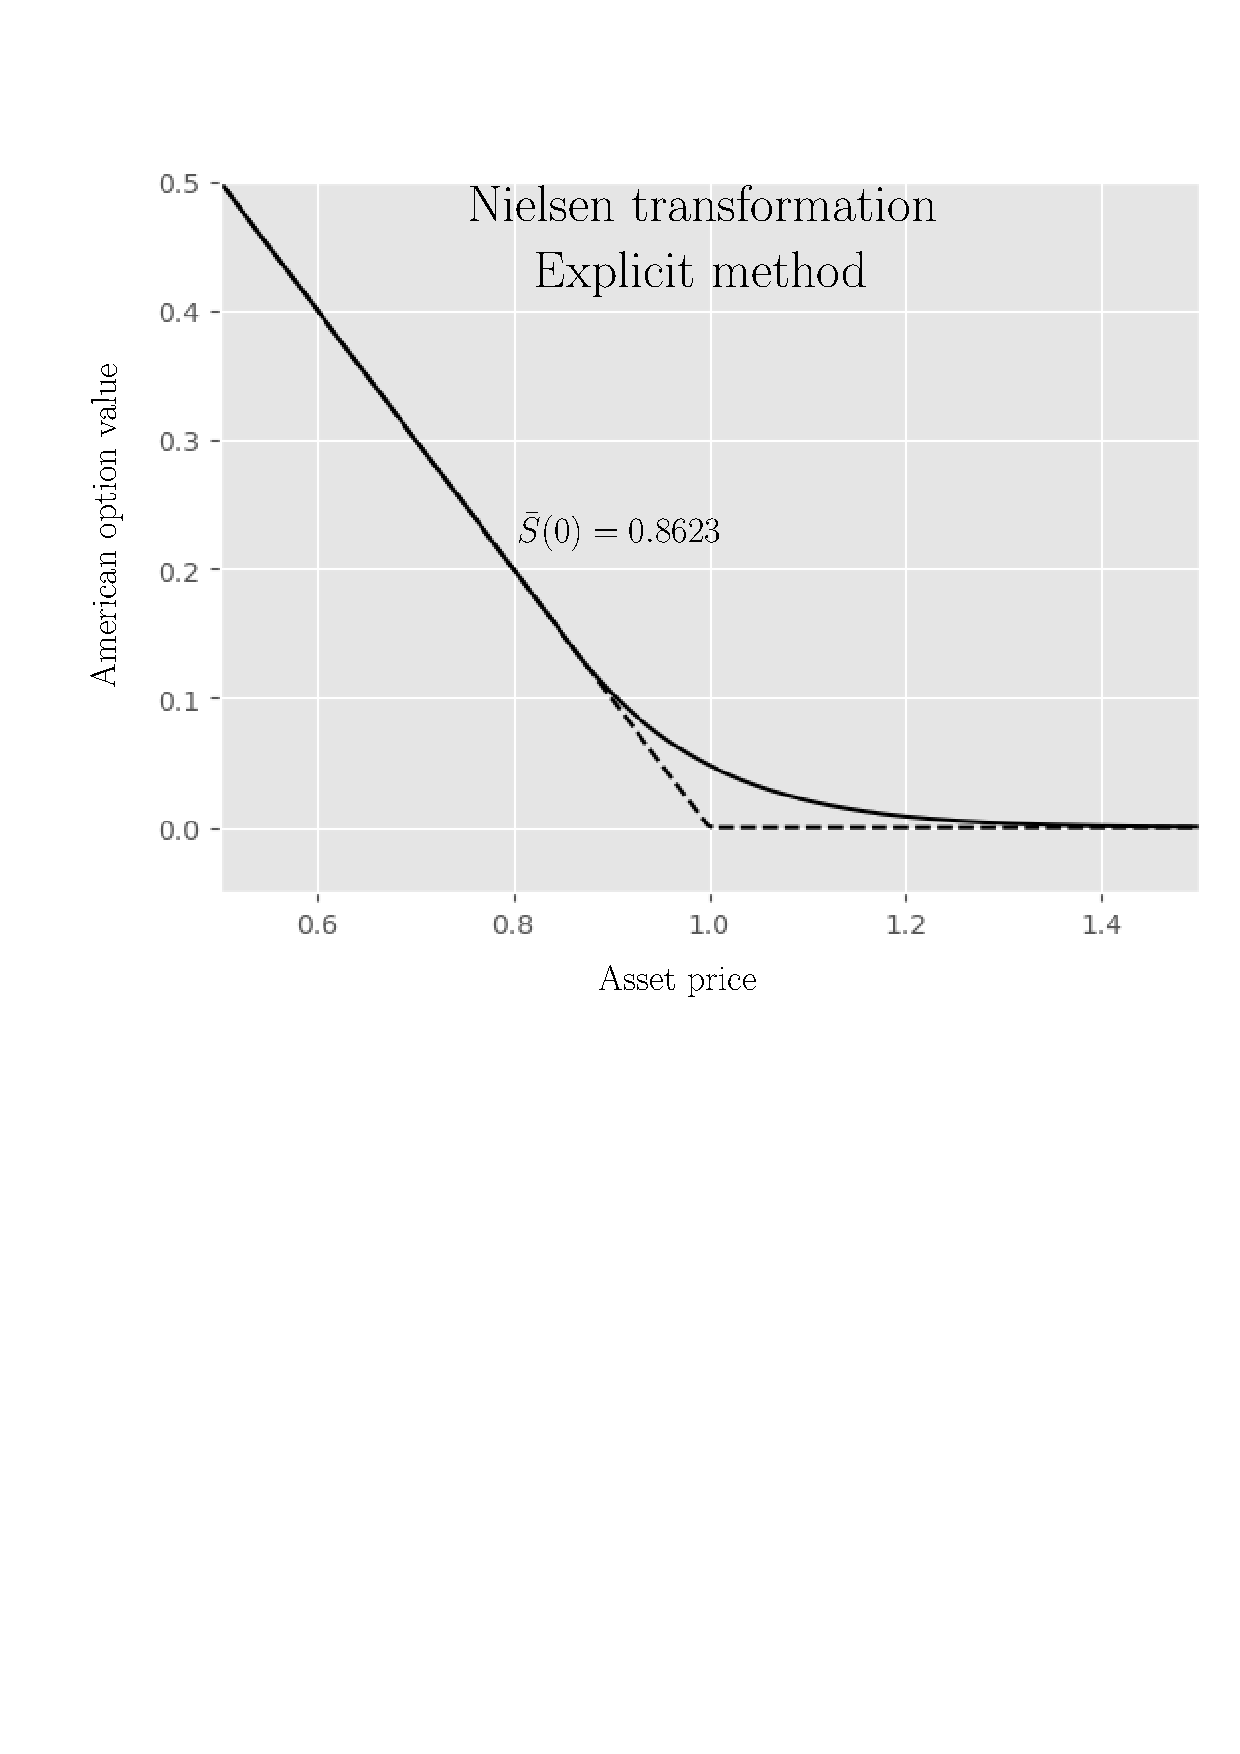
\includegraphics[width=\textwidth]{chapters/chapter3/TestCase2NielsenExplicit.pdf}
    \caption{$\Delta{x}=\expnumber{1}{-3}, \Delta{t}=0.5\times\expnumber{1}{-6}$}
    \label{fig:finitedifferencesschemes:numericaresults:test_case_2_explicit_nielsen}
  \end{subfigure}
  \hspace{0.5cm}
  \begin{subfigure}{0.4\textwidth}
    \label{fig:finitedifferencesschemes:numericaresults:test_case_2_implicit_nielsen}
    \centering
    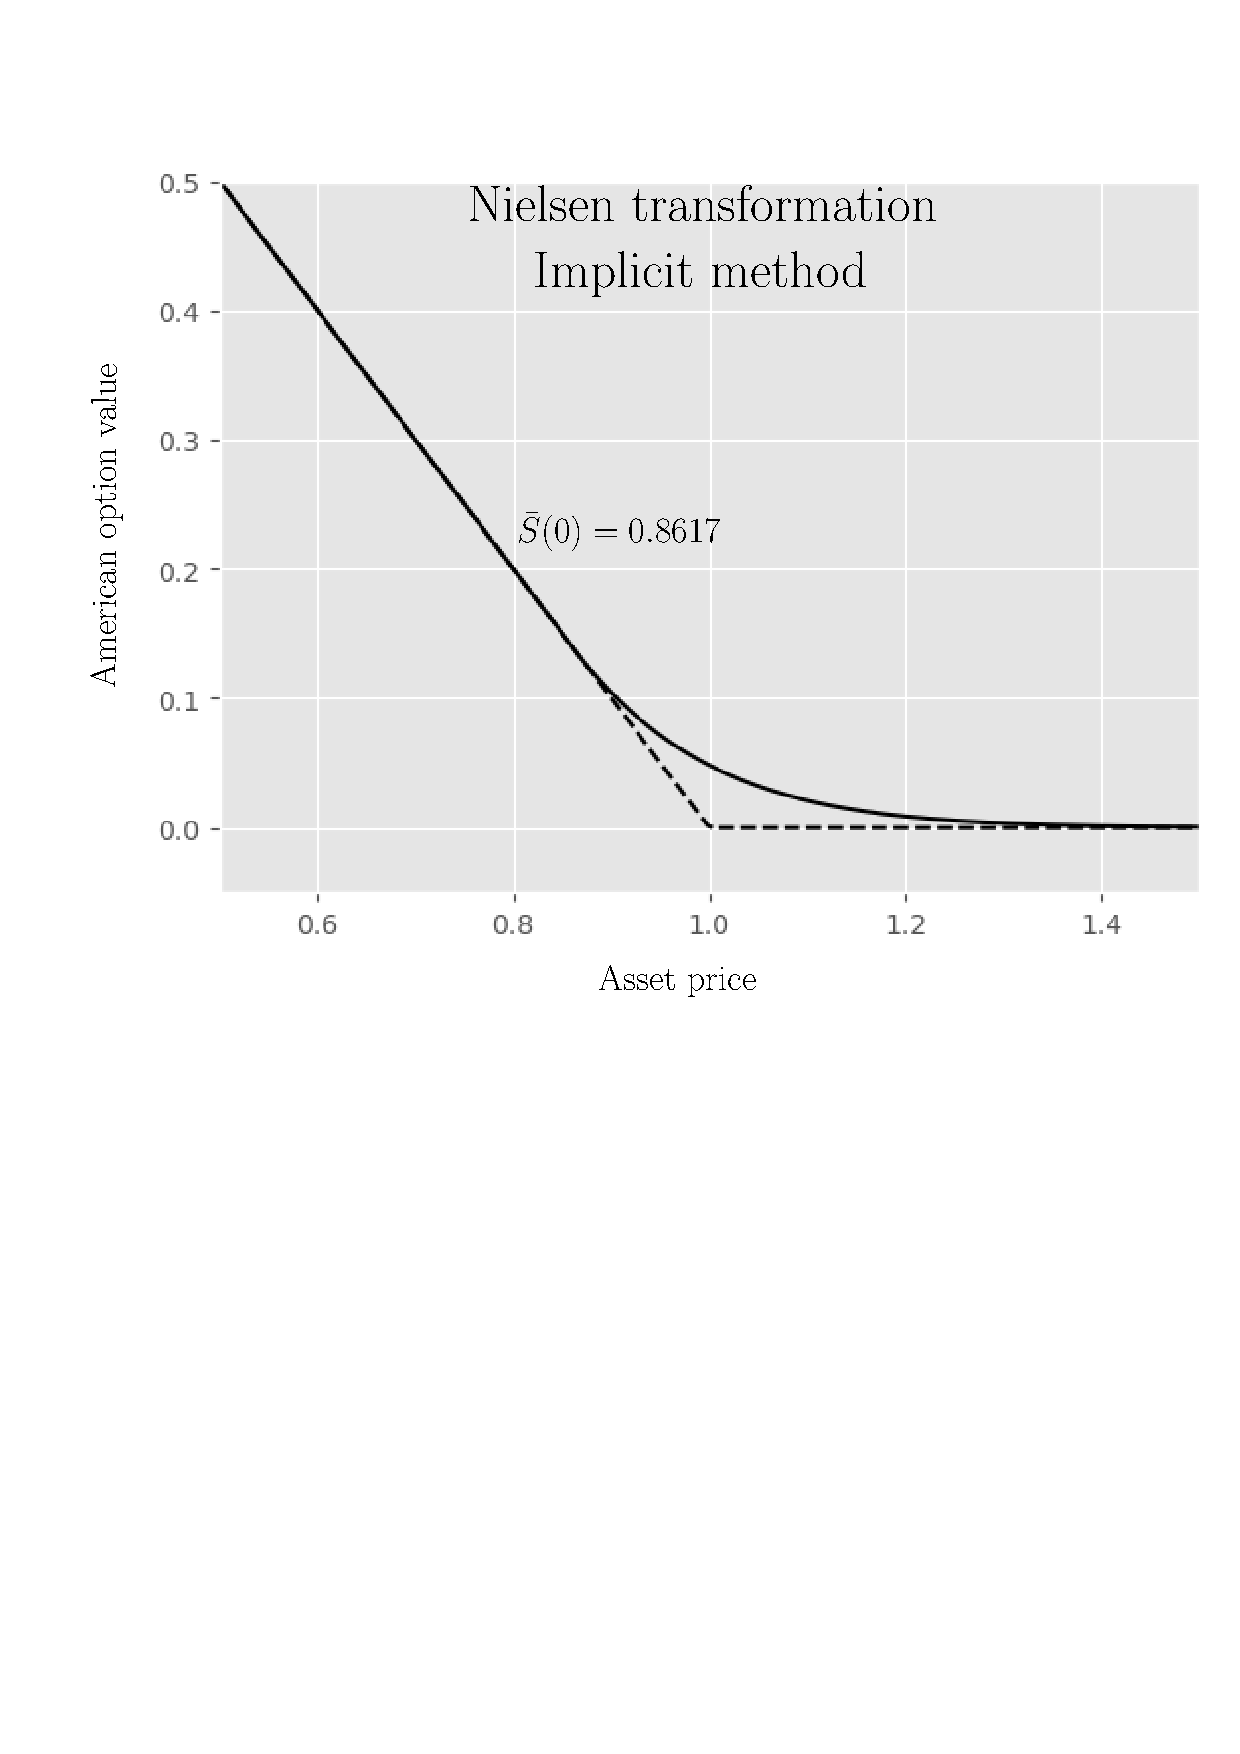
\includegraphics[width=\textwidth]{chapters/chapter3/TestCase2NielsenImplicit.pdf}
    \caption{$\Delta{x}=\Delta{t}=\expnumber{1}{-3}$.}
  \end{subfigure}
  \caption{American put option value $V(S, 0)$ curve.}
  \label{fig:finitedifferencesschemes:numericaresults:test_case_2}
\end{figure}

% Please add the following required packages to your document preamble:
% \usepackage{booktabs}
\begin{table}[H]
    \centering
    \begin{tabular}{@{}ccccccc@{}}
    \toprule
    \textbf{Asset price} & \textbf{BOPM} & 0.125    & 0.0625   & 0.03125  & 0.015625 & 0.0078125 \\ \midrule
    0.8                  & 0.200000      & 0.200000 & 0.200000 & 0.200000 & 0.200000 & 0.200000  \\
    1.0                  & 0.048167      & 0.049286 & 0.049274 & 0.048465 & 0.048256 & 0.048174  \\
    1.2                  & 0.008666      & 0.010736 & 0.009108 & 0.008829 & 0.008686 & 0.008667  \\
    1.4                  & 0.001285      & 0.001950 & 0.001501 & 0.001349 & 0.001295 & 0.001287  \\
    1.6                  & 0.000167      & 0.000354 & 0.000224 & 0.000185 & 0.000172 & 0.000168  \\
    1.8                  & 0.000020      & 0.000076 & 0.000035 & 0.000024 & 0.000021 & 0.000020  \\
    2.0                  & 0.000002      & 0.000017 & 0.000006 & 0.000003 & 0.000003 & 0.000002  \\
    & \textbf{RSME} & 0.000092 & 0.000045 & 0.000013 & 0.000003 & 0.00000   \\ \bottomrule
    \end{tabular}
    \caption{\label{tab:rsme_explicit_company_transformation}RSME error produced by the explicit scheme for Company transformation for $\Delta{t}=1/8,1/16,\dots,1/128$ and $\Delta{t}=\Delta{x}^2/2$.}
\end{table}
Additionally, we proceeded to the case for call and put options with dividends. We used the same set of parameters \eqref{eq:numericaresults:parameters_set_1} but with the slight modification so that the underlying asset pays dividends
\begin{equation}
  \label{eq:numericaresults:parameters_set_2}
  K = 1, \quad T = 1, \quad r=0.2, \quad \sigma=0.2, \quad \delta = 0.03
\end{equation}
In table \eqref{tab:rsme_explicit_company_transformation_put}, we present the approximation error produced by the explicit method for the Nielsen transformation, and in figure \eqref{fig:finitedifferencesschemes:numericaresults:test_case_4}, it is shown the value curve obtained for each of the methods with parameters \eqref{eq:numericaresults:parameters_set_2}. See appendix \eqref{sec:numericalexperiments} for the same experiments for call options.

\begin{figure}[tbp]
  \centering
  \begin{subfigure}{0.4\textwidth}
    \centering
    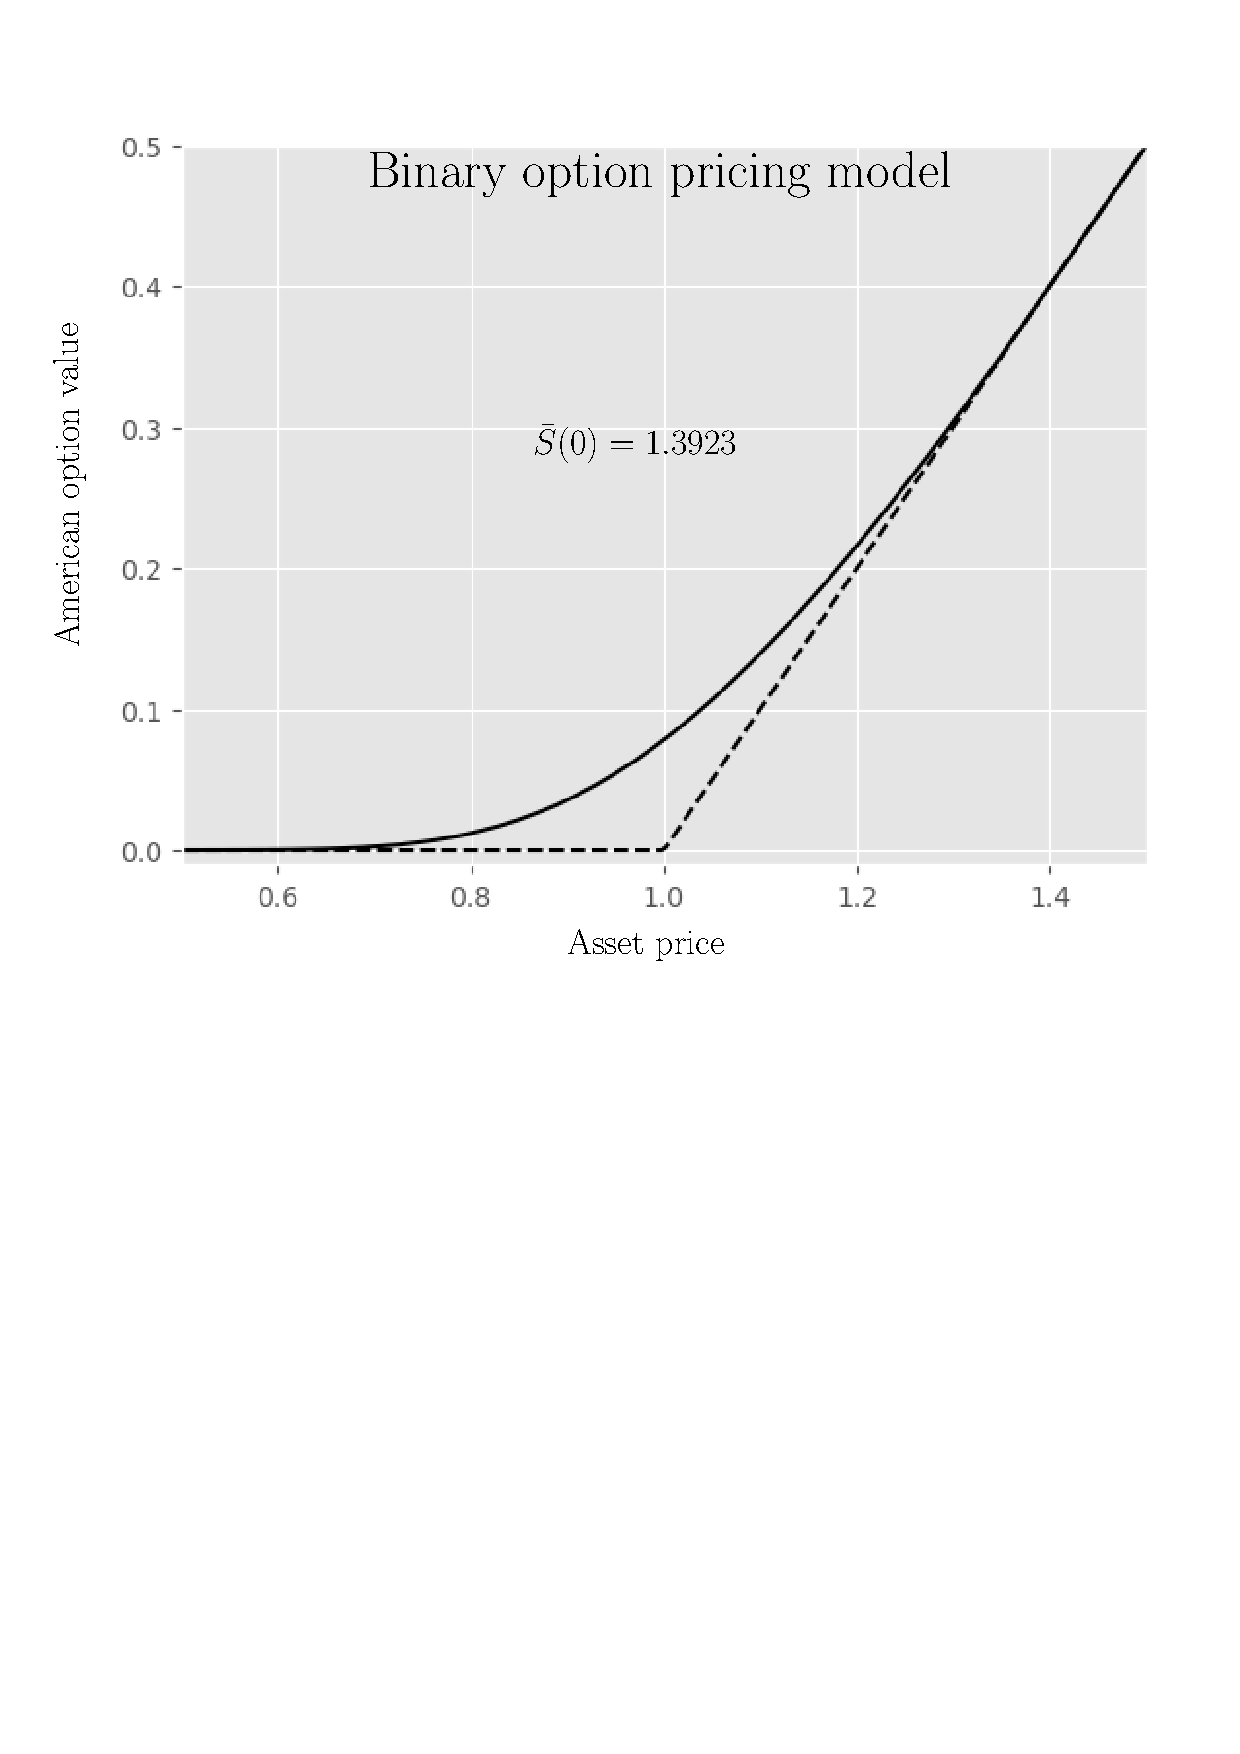
\includegraphics[width=\textwidth]{chapters/chapter3/TestCase3BOPM.pdf}
    \caption{$\text{Nodes} = 2^{500}$.}
    \label{fig:finitedifferencesschemes:numericaresults:test_case_4_bopm}
  \end{subfigure}
  \hspace{0.5cm}
  \begin{subfigure}{0.4\textwidth}
    \centering
    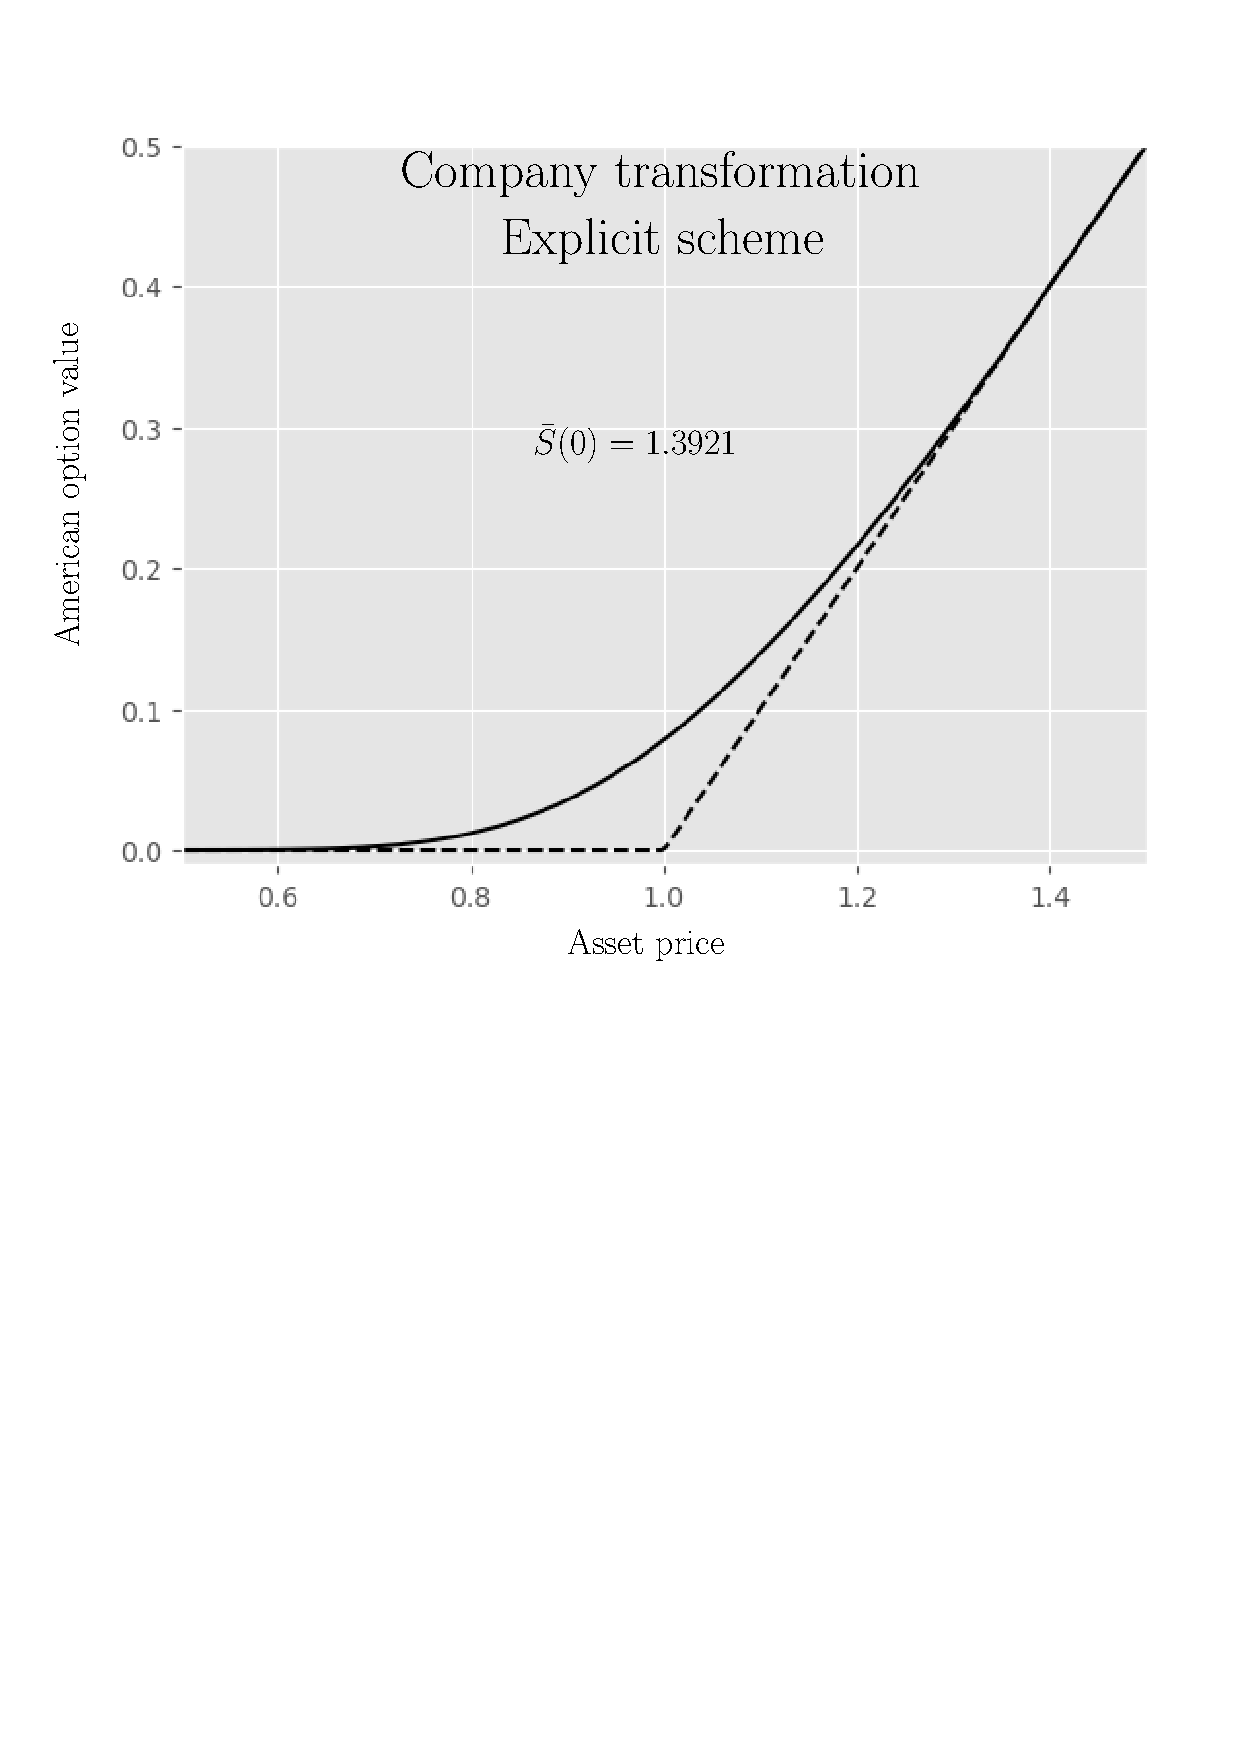
\includegraphics[width=\textwidth]{chapters/chapter3/TestCase3ExplicitCompany.pdf}
    \caption{$\Delta{x}=\expnumber{1}{-3}, \Delta{t}=0.5\times\expnumber{1}{-6}$}
    \label{fig:finitedifferencesschemes:numericaresults:test_case_4_explicit_company}
  \end{subfigure}
  \begin{subfigure}{0.4\textwidth}
    \centering
    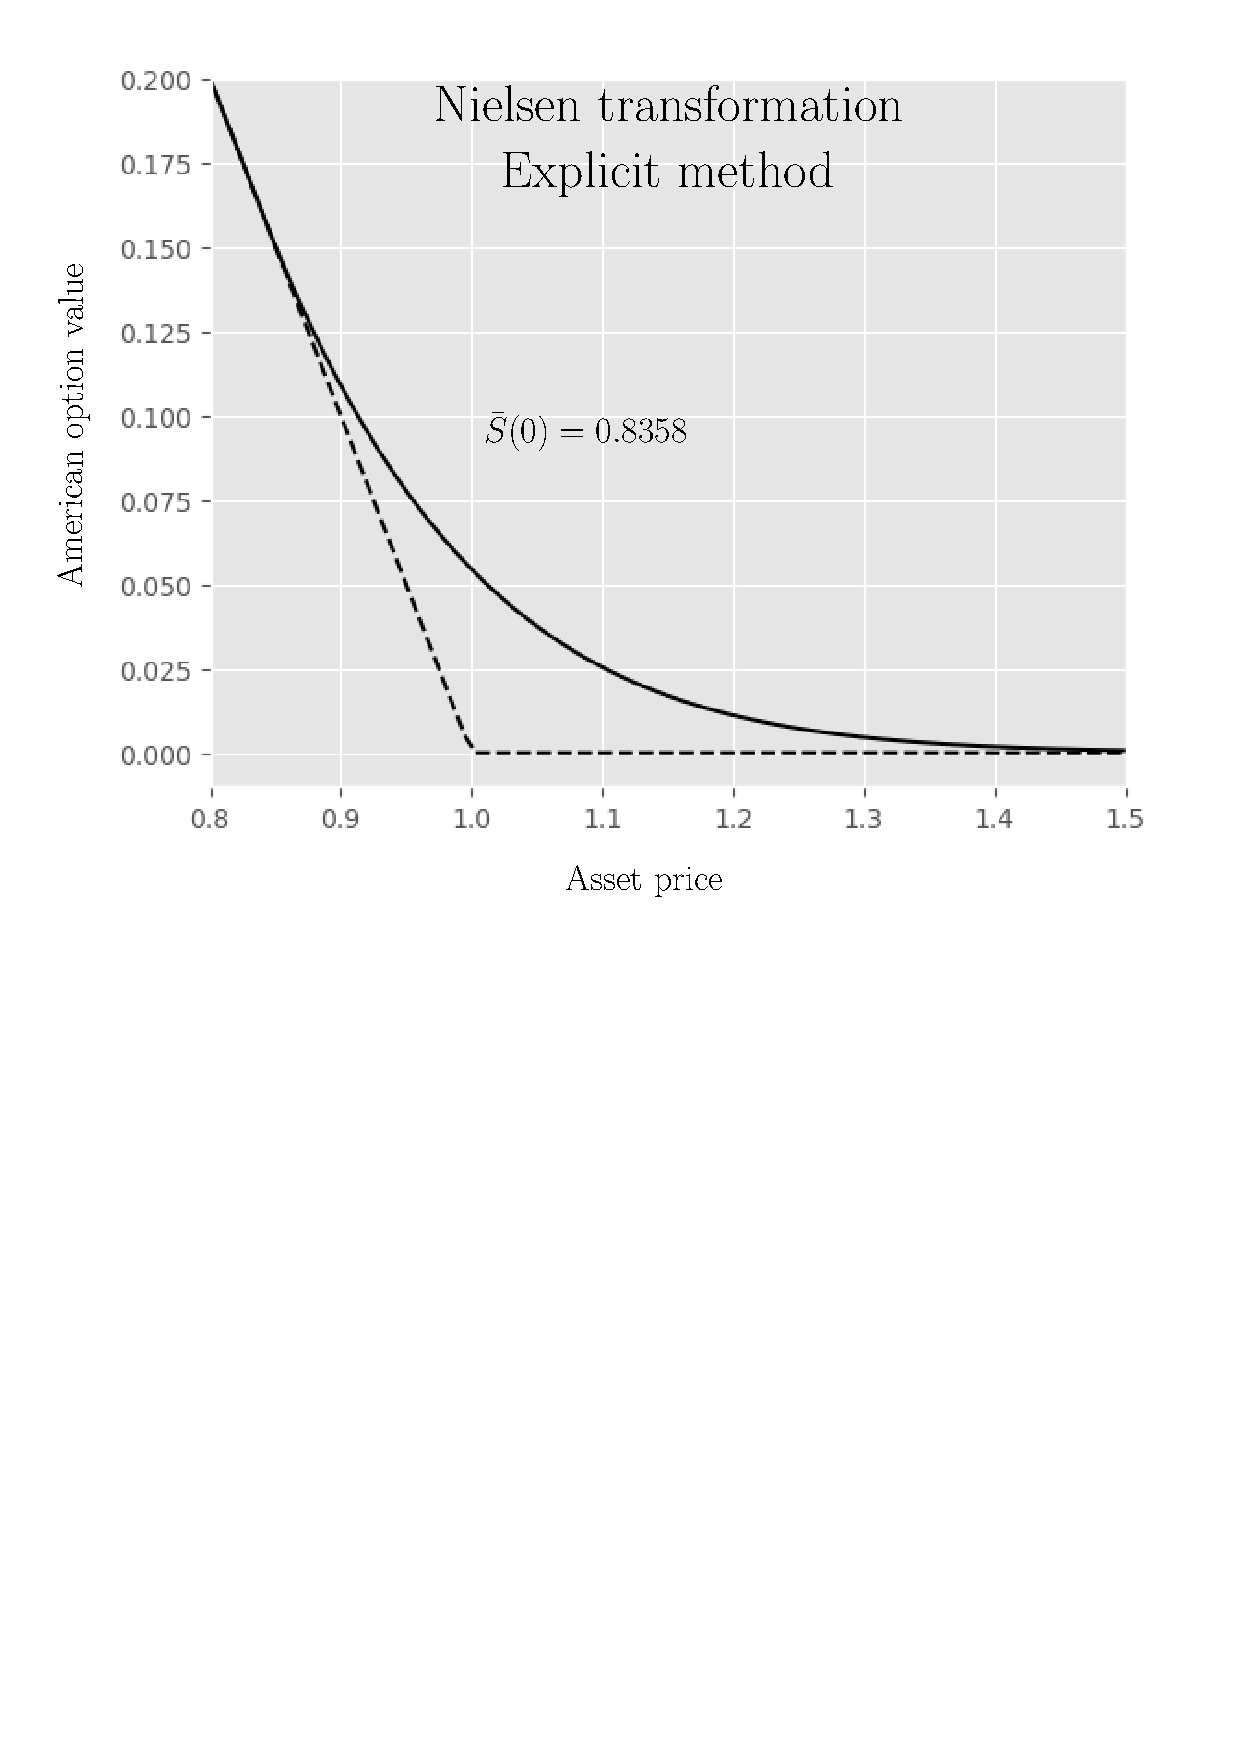
\includegraphics[width=\textwidth]{chapters/chapter3/TestCase3ExplicitNielsen.pdf}
    \caption{$\Delta{x}=\expnumber{1}{-3}, \Delta{t}=0.5\times\expnumber{1}{-6}$}
    \label{fig:finitedifferencesschemes:numericaresults:test_case_4_explicit_nielsen}
  \end{subfigure}
  \hspace{0.5cm}
  \begin{subfigure}{0.4\textwidth}
    \label{fig:finitedifferencesschemes:numericaresults:test_case_4_implicit_nielsen}
    \centering
    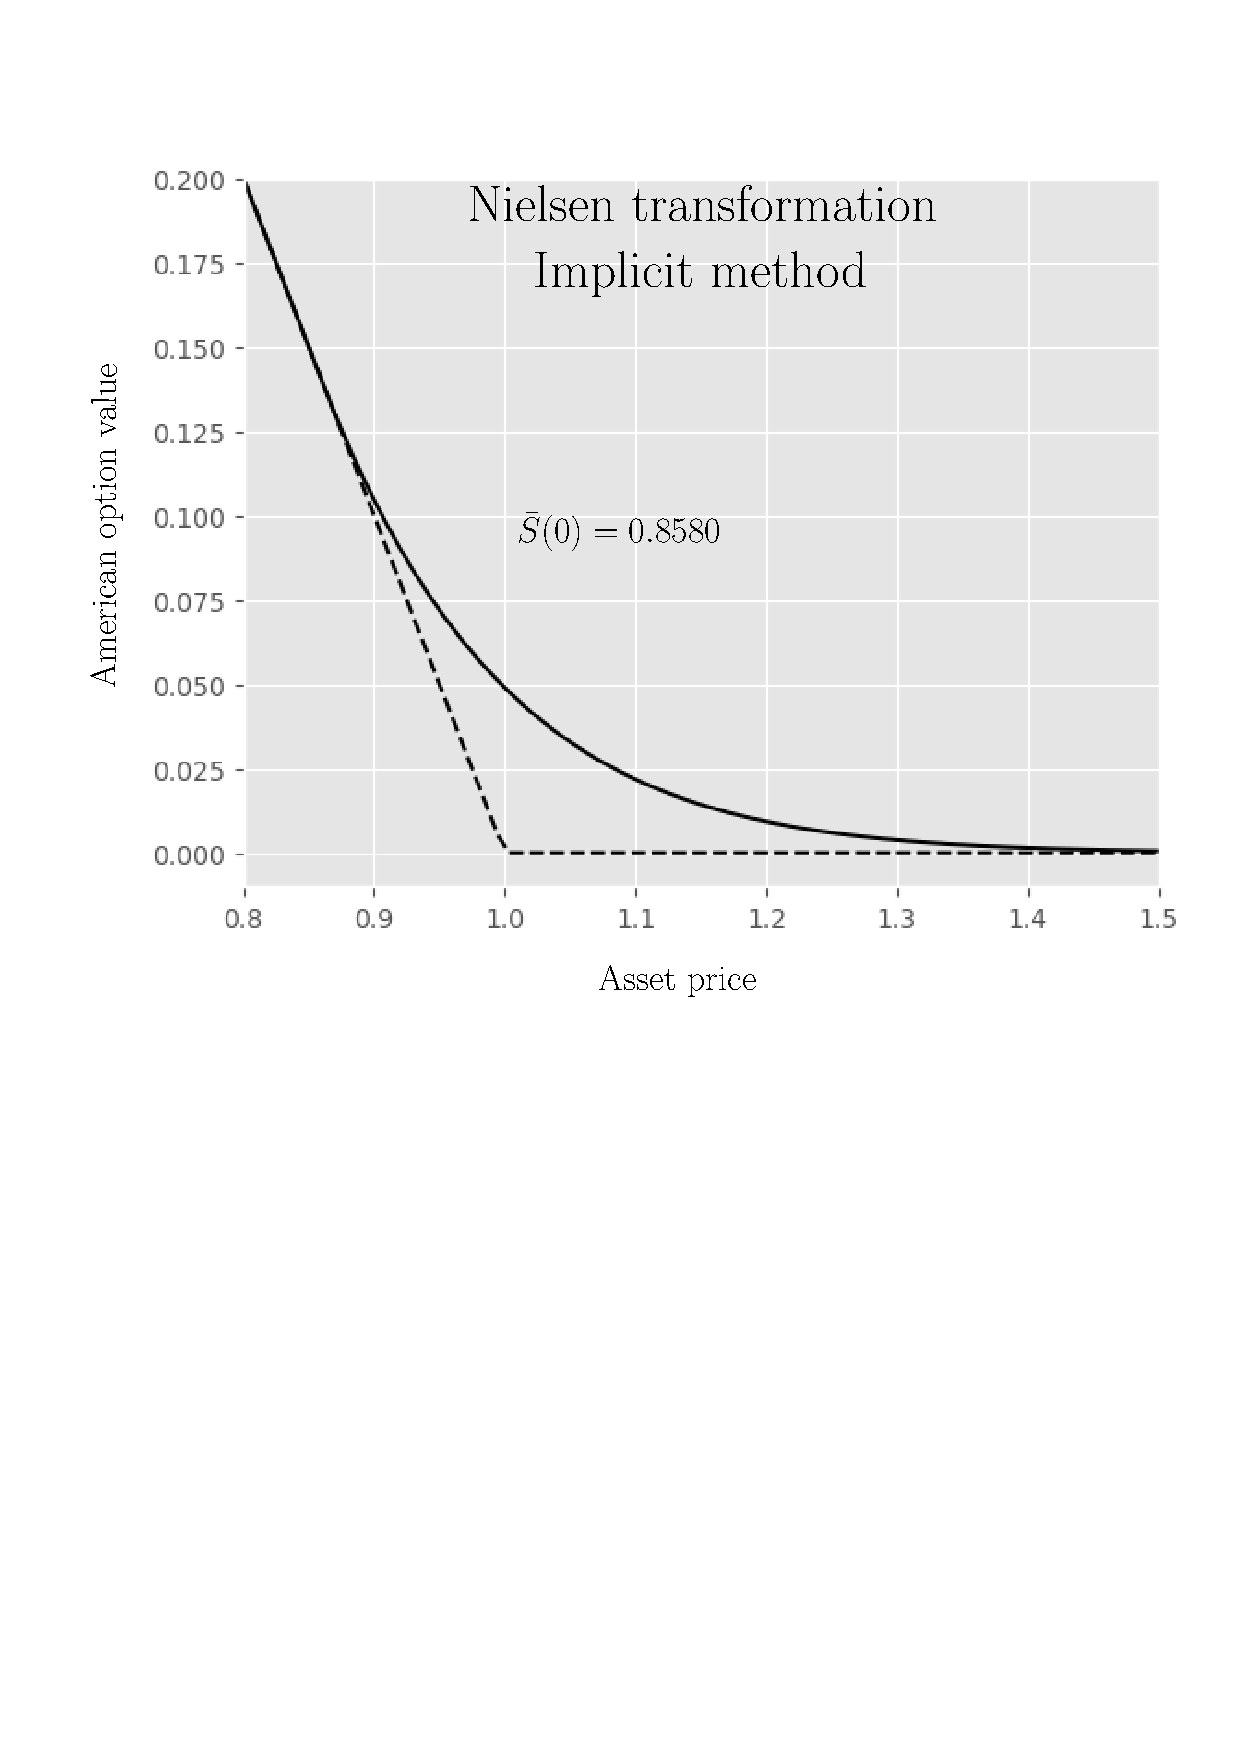
\includegraphics[width=\textwidth]{chapters/chapter3/TestCase3ImplictNielsen.pdf}
    \caption{$\Delta{x}=\Delta{t}=\expnumber{1}{-3}$.}
  \end{subfigure}
  \caption{American put option value $V(S, 0)$ curve.}
  \label{fig:finitedifferencesschemes:numericaresults:test_case_4}
\end{figure}

% Please add the following required packages to your document preamble:
% \usepackage{booktabs}
\begin{table}[H]
  \centering
  \begin{tabular}{@{}ccccccc@{}}
  \toprule
  \textbf{Asset price} & \textbf{BOPM} & 0.125    & 0.0625   & 0.03125  & 0.015625 & 0.0078125                    \\ \midrule
  0.8                  & 0.200000      & 0.200000 & 0.200000 & 0.200000 & 0.200000 & 0.200000                     \\
  1.0                  & 0.054464      & 0.053355 & 0.054588 & 0.054501 & 0.054465 & 0.054469                     \\
  1.2                  & 0.011255      & 0.011585 & 0.011457 & 0.011255 & 0.011179 & 0.011161                     \\
  1.4                  & 0.001855      & 0.002219 & 0.002006 & 0.001889 & 0.001857 & 0.001847                     \\
  1.6                  & 0.000262      & 0.000399 & 0.000315 & 0.000277 & 0.000268 & 0.000265                     \\
                       & \textbf{RSME} & 0.00041  & 0.000010 & 0.000002 & 0.000002 & \multicolumn{1}{l}{0.000003} \\ \bottomrule
  \end{tabular}
  \caption{\label{tab:rsme_explicit_company_transformation_put}RSME error produced by the explicit scheme for Nielsen transformation to approximate put option \eqref{eq:numericaresults:parameters_set_2} given $\Delta{t}=1/8,1/16,\dots,1/128$ and $\Delta{t}=\Delta{x}^2/2$.}
  \end{table}

Finally, we conducted a convergence analysis to determine the order of convergence of each the methods. For simplicity, the numerical experiment was conducted for put options and with parameters \eqref{eq:numericaresults:parameters_set_2}. However, we expect that numerical experiment will yield similar results for call options and other set of parameters. Moreover, for analyzing the convergence, we are taking the relative error between contiguous grid in sizes. Specifically, to determine the order of convergence in space, we define the grids with resolution $\Delta{x}_i=h/2^i$ for $i=0,\dots,3$ while $\Delta{t}$ is fixed. Conversely, to determine the temporal order of convergence, we vary $\Delta{t}$ and fix $\Delta{x}$ in similar way. Therefore, the error between consecutive grids is defined as
\begin{equation}
  \mathbf{e}_k = ||\mathbf{v}_{k+1} - \mathbf{v}_{k}||_{\infty} \quad \text{for $k=0,\dots,3$}
  \label{eq:finitedifferencesschemes:numericalresults:consecutive_error}
\end{equation}
where $\mathbf{v}_{k}\in\mathbb{R}^{M+1}$ is the vector with the approximation produced by our method and $||\cdot||_{\infty}$ is the infinity norm. In figure \eqref{fig:finitedifferencesschemes:numericaresults:nielsen_convergence analysis}, we show log-log plots of the error produced by the explicit and implicit methods for Nielsen transformation. As you can see, both explicit and implicit methods have first order convergence in space. Recall that although we are using central finite difference, the Nielsen schemes use forward (or backward for calls) difference to approximate the contact point condition \eqref{eq:finitedifferencesschemes:explicit:contact_point_approximation_2} which is first order in space, hence, degrading the overall convergence of the method. In the other hand, figure \eqref{fig:finitedifferencesschemes:numericaresults:company_convergence analysis} shows the convergence order for the explicit method for the Company transformation. Contrary to Nielsen's schemes, the explicit method for Company transformation is second order in space. This is because Company uses a central finite difference scheme for approximating the contact point condition \eqref{eq:appendix:explicitmethodcompany:contact_point_approximation}. Moreover, all methods are first order convergence in space as suggested by the forward/backward difference approximation used for the temporal axis.
\begin{figure}[tbp]
  \centering
  \begin{subfigure}{0.4\textwidth}
    \centering
    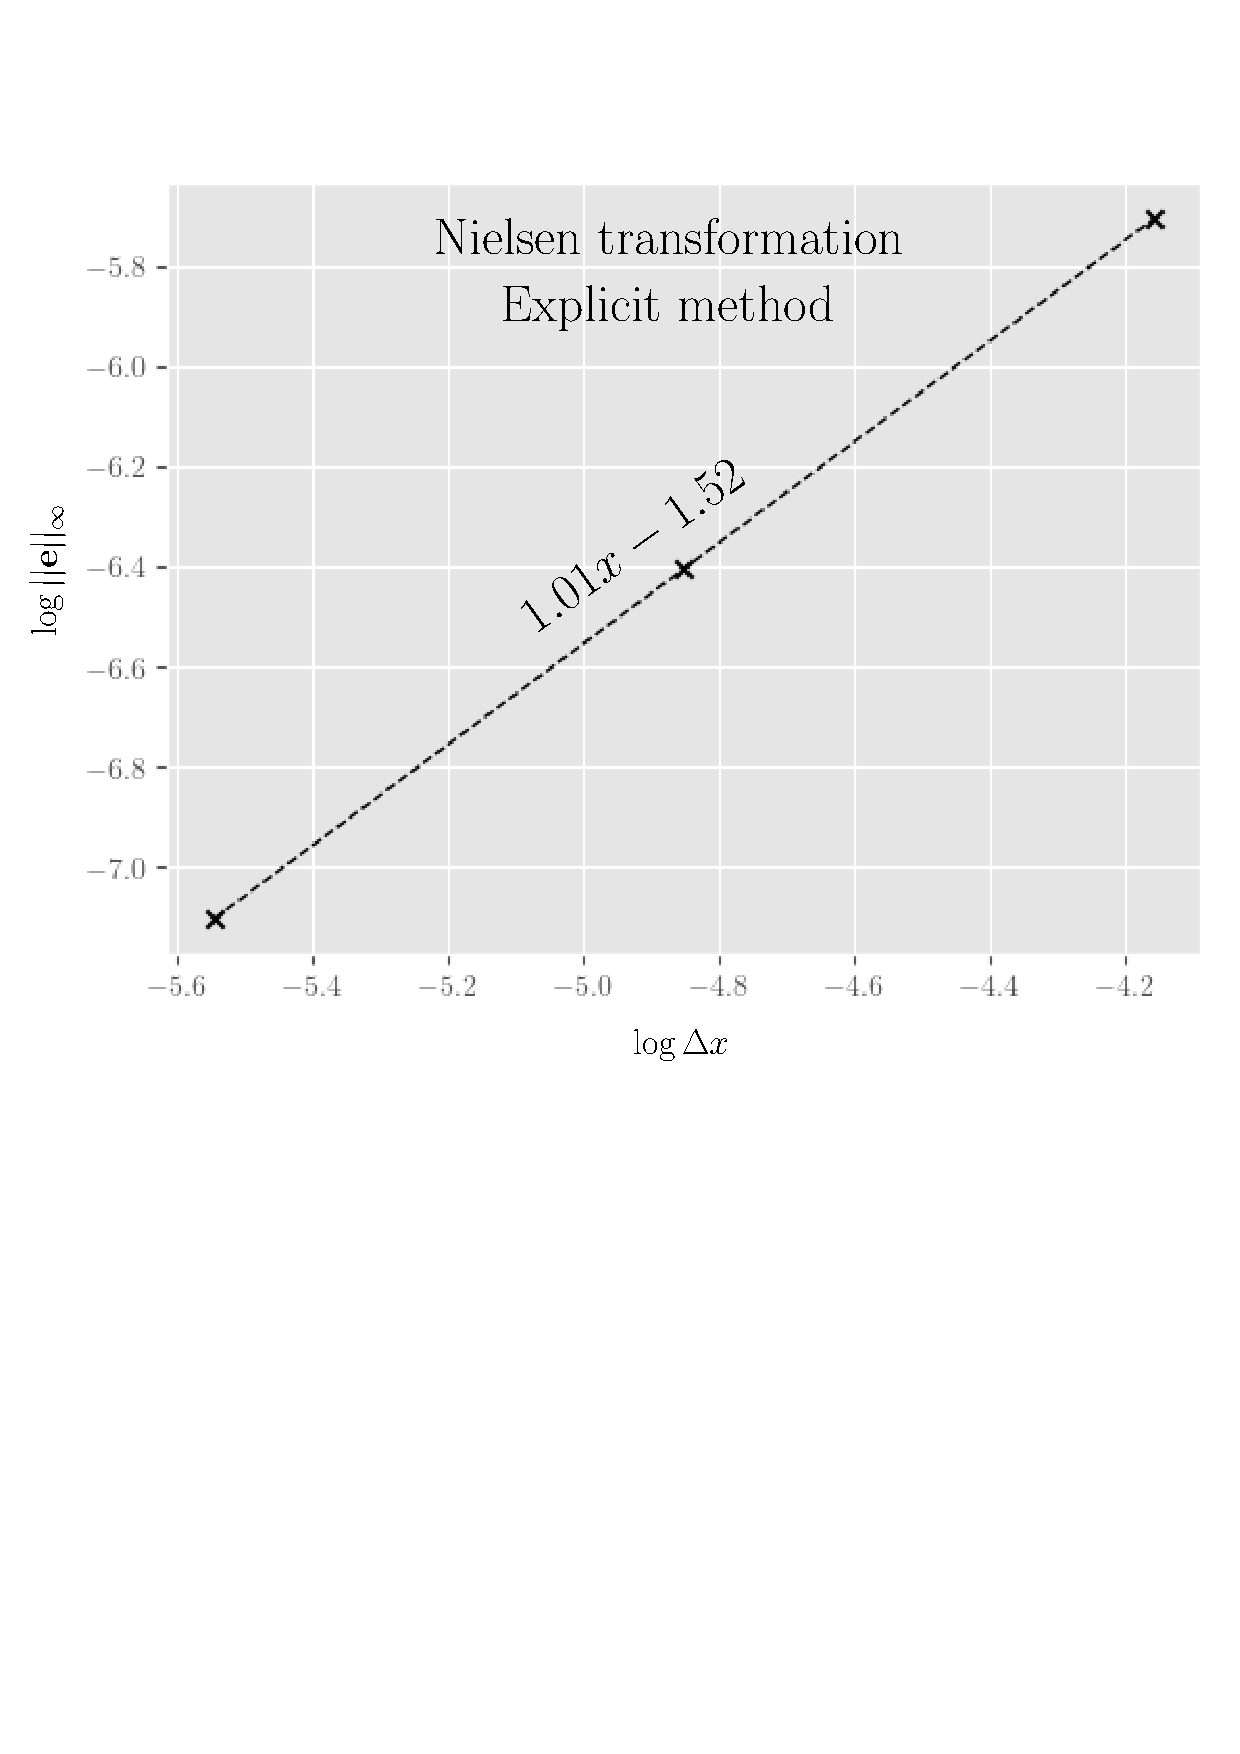
\includegraphics[width=\textwidth]{chapters/chapter3/ConvergenceSpaceExplicitNielsen.pdf}
    \caption{$\Delta{x}=2^{-7},\dots,2^{-10}$}
    \caption*{$\Delta{t}=2^{-21}$}
    \label{fig:finitedifferencesschemes:numericaresults:nielsen_explicit_space}
  \end{subfigure}
  \hspace{0.5cm}
  \begin{subfigure}{0.4\textwidth}
    \centering
    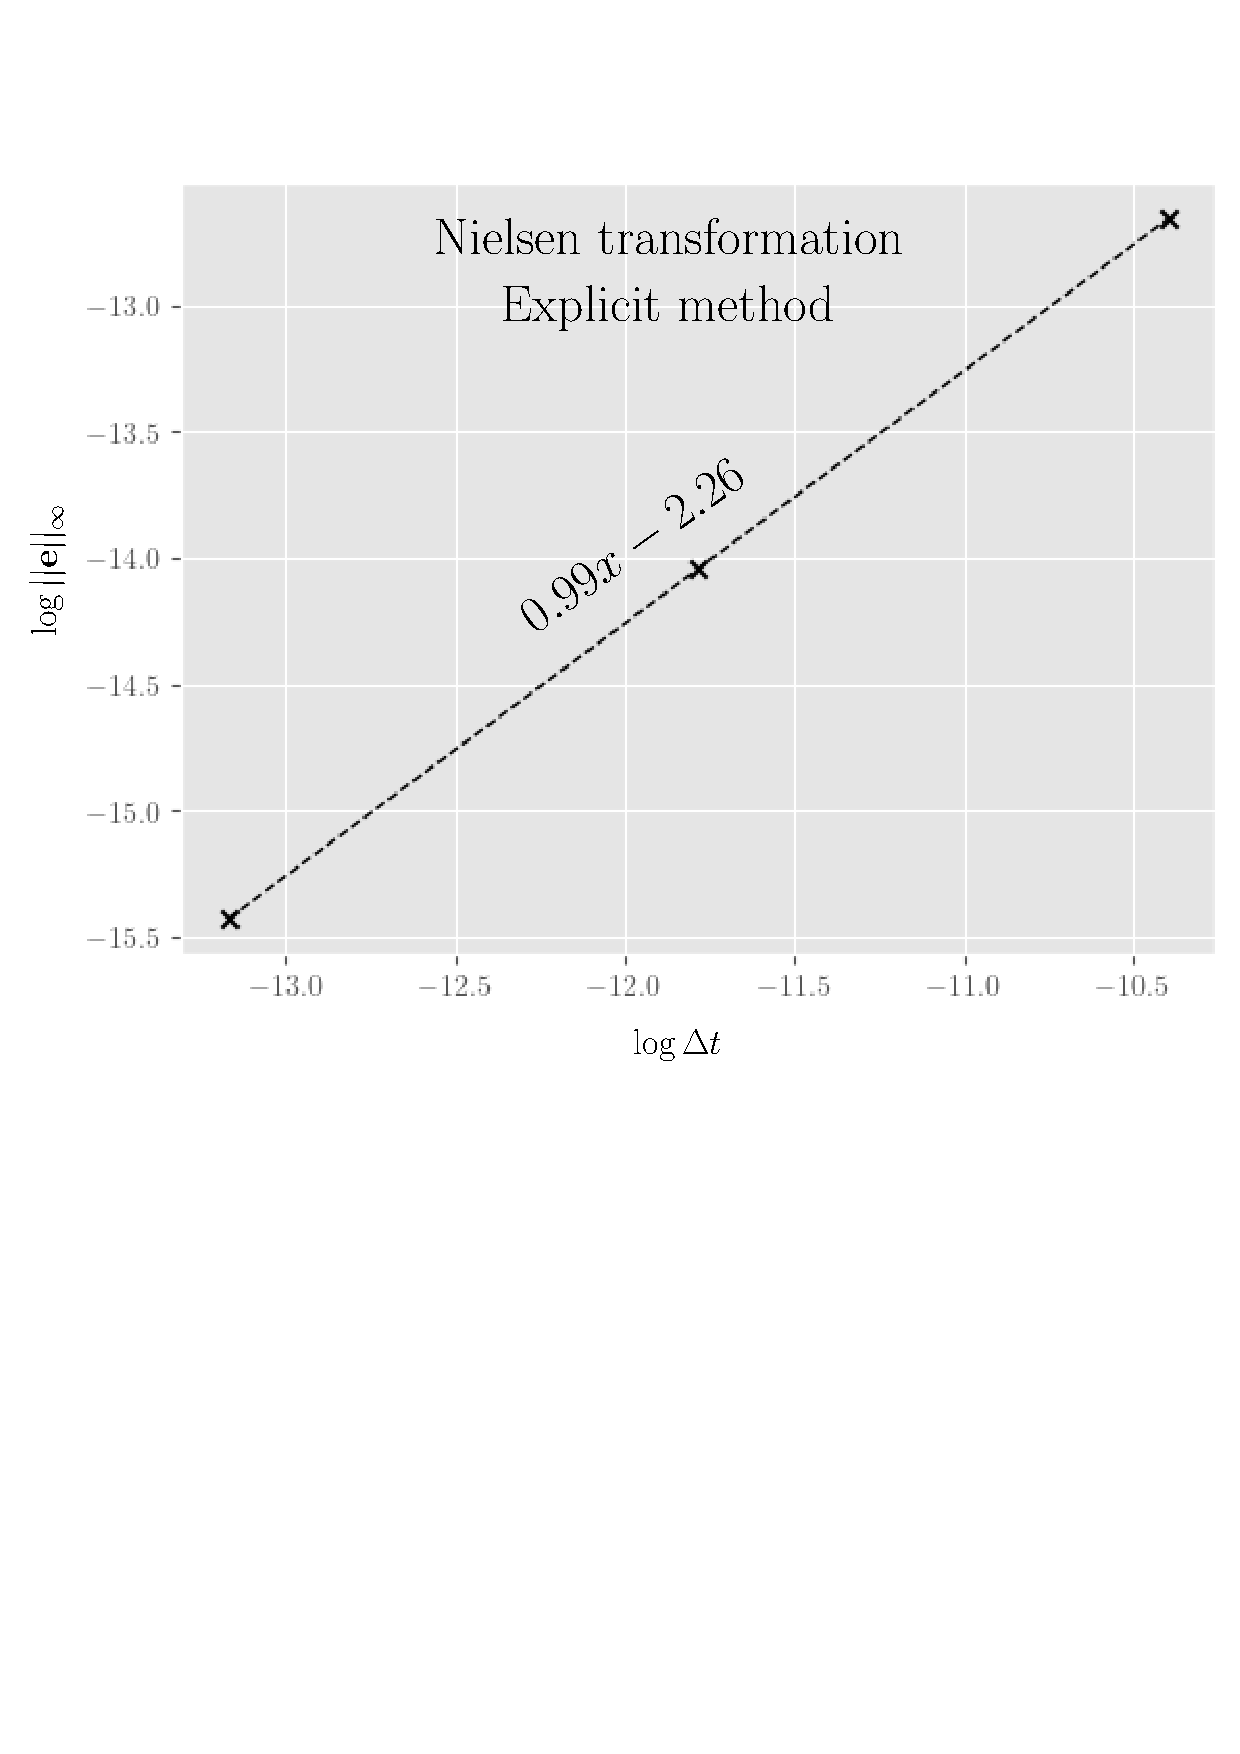
\includegraphics[width=\textwidth]{chapters/chapter3/ConvergenceTimeExplicitNielsen.pdf}
    \caption{$\Delta{t}=2^{-15},2^{-17},\dots,2^{-21}$}
    \caption*{$\Delta{x}=2^{-7}$}
    \label{fig:finitedifferencesschemes:numericaresults:nielsen_explicit_time}
  \end{subfigure}
  \begin{subfigure}{0.4\textwidth}
    \centering
    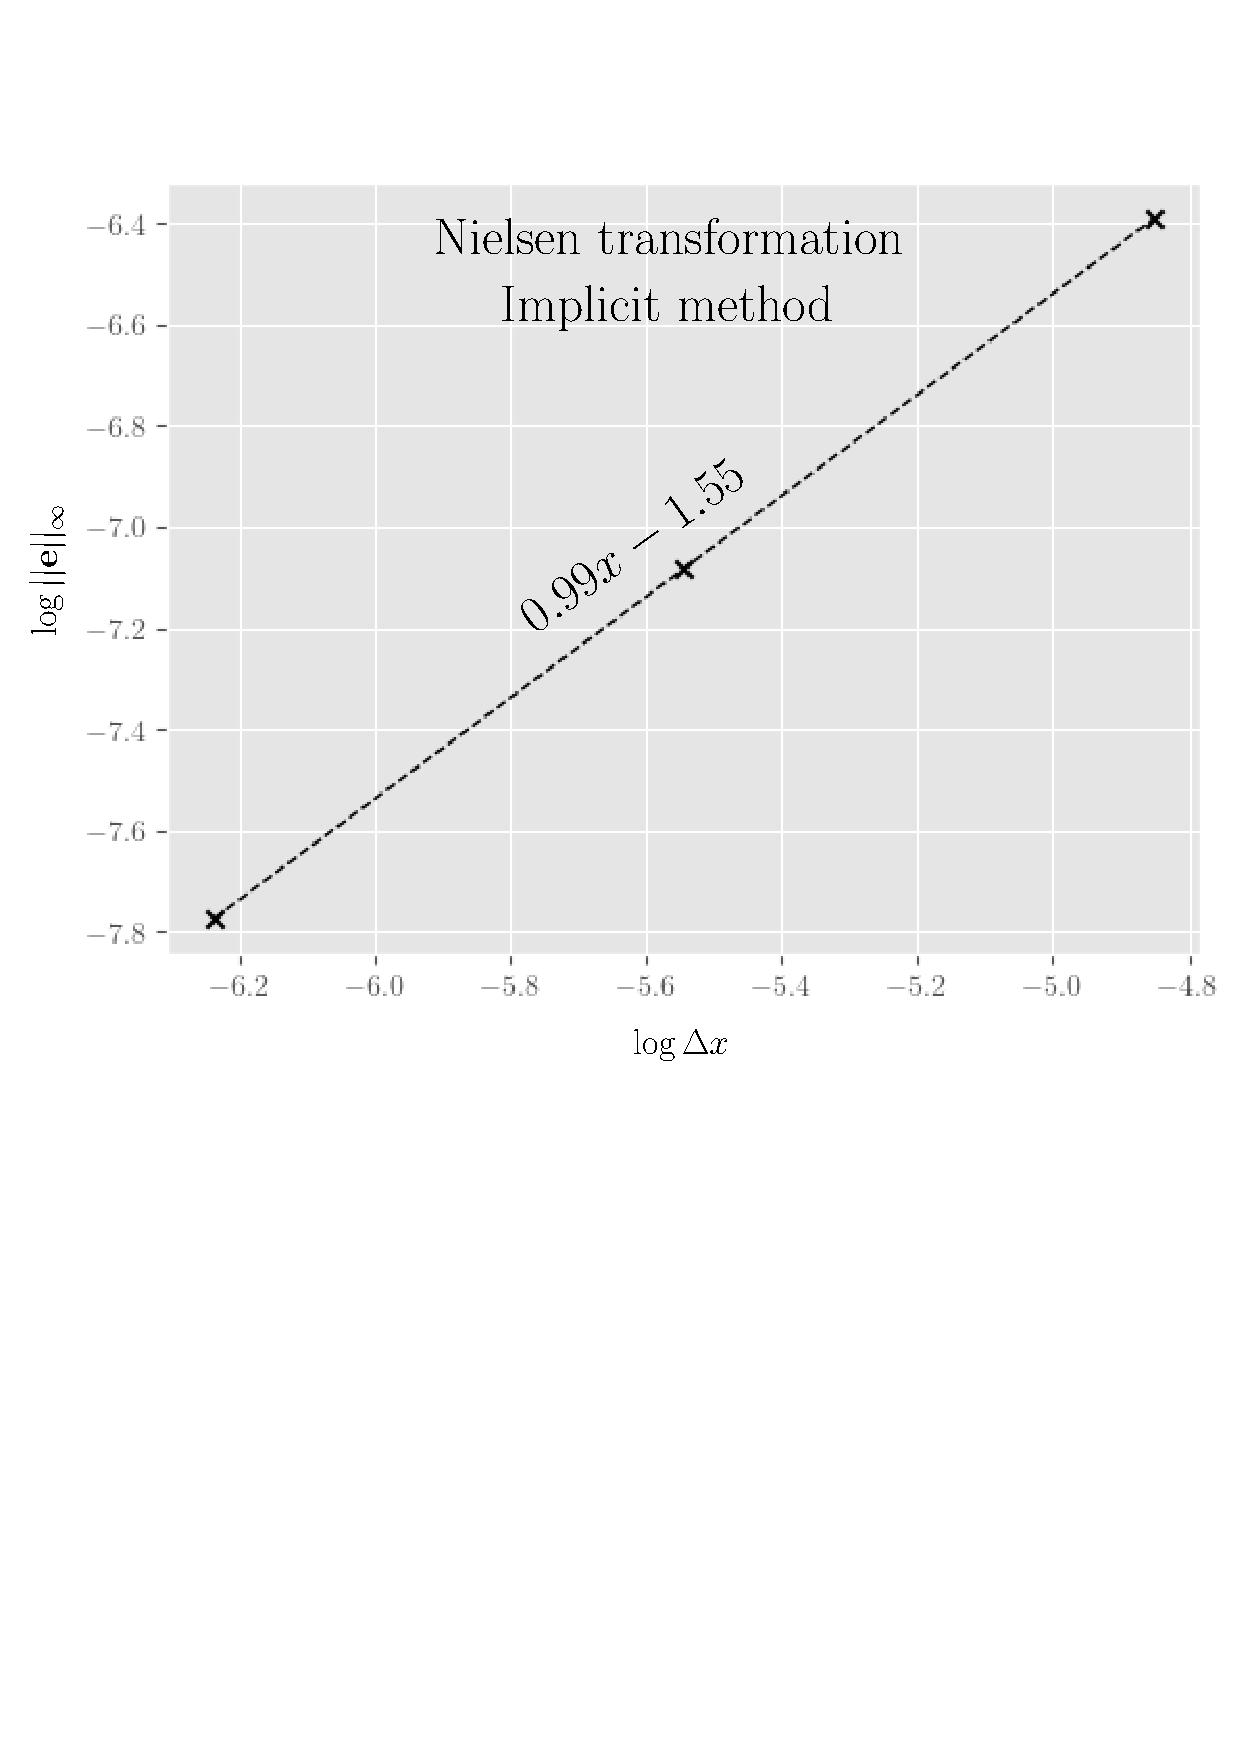
\includegraphics[width=\textwidth]{chapters/chapter3/ConvergenceSpaceImplicitNielsen.pdf}
    \caption{$\Delta{x}=2^{-6},\dots,2^{-8}$}
    \caption*{$\Delta{t}=2^{-2}$}
    \label{fig:finitedifferencesschemes:numericaresults:nielsen_implicit_space}
  \end{subfigure}
  \hspace{0.5cm}
  \begin{subfigure}{0.4\textwidth}
    \label{fig:finitedifferencesschemes:numericaresults:nielsen_implicit_time}
    \centering
    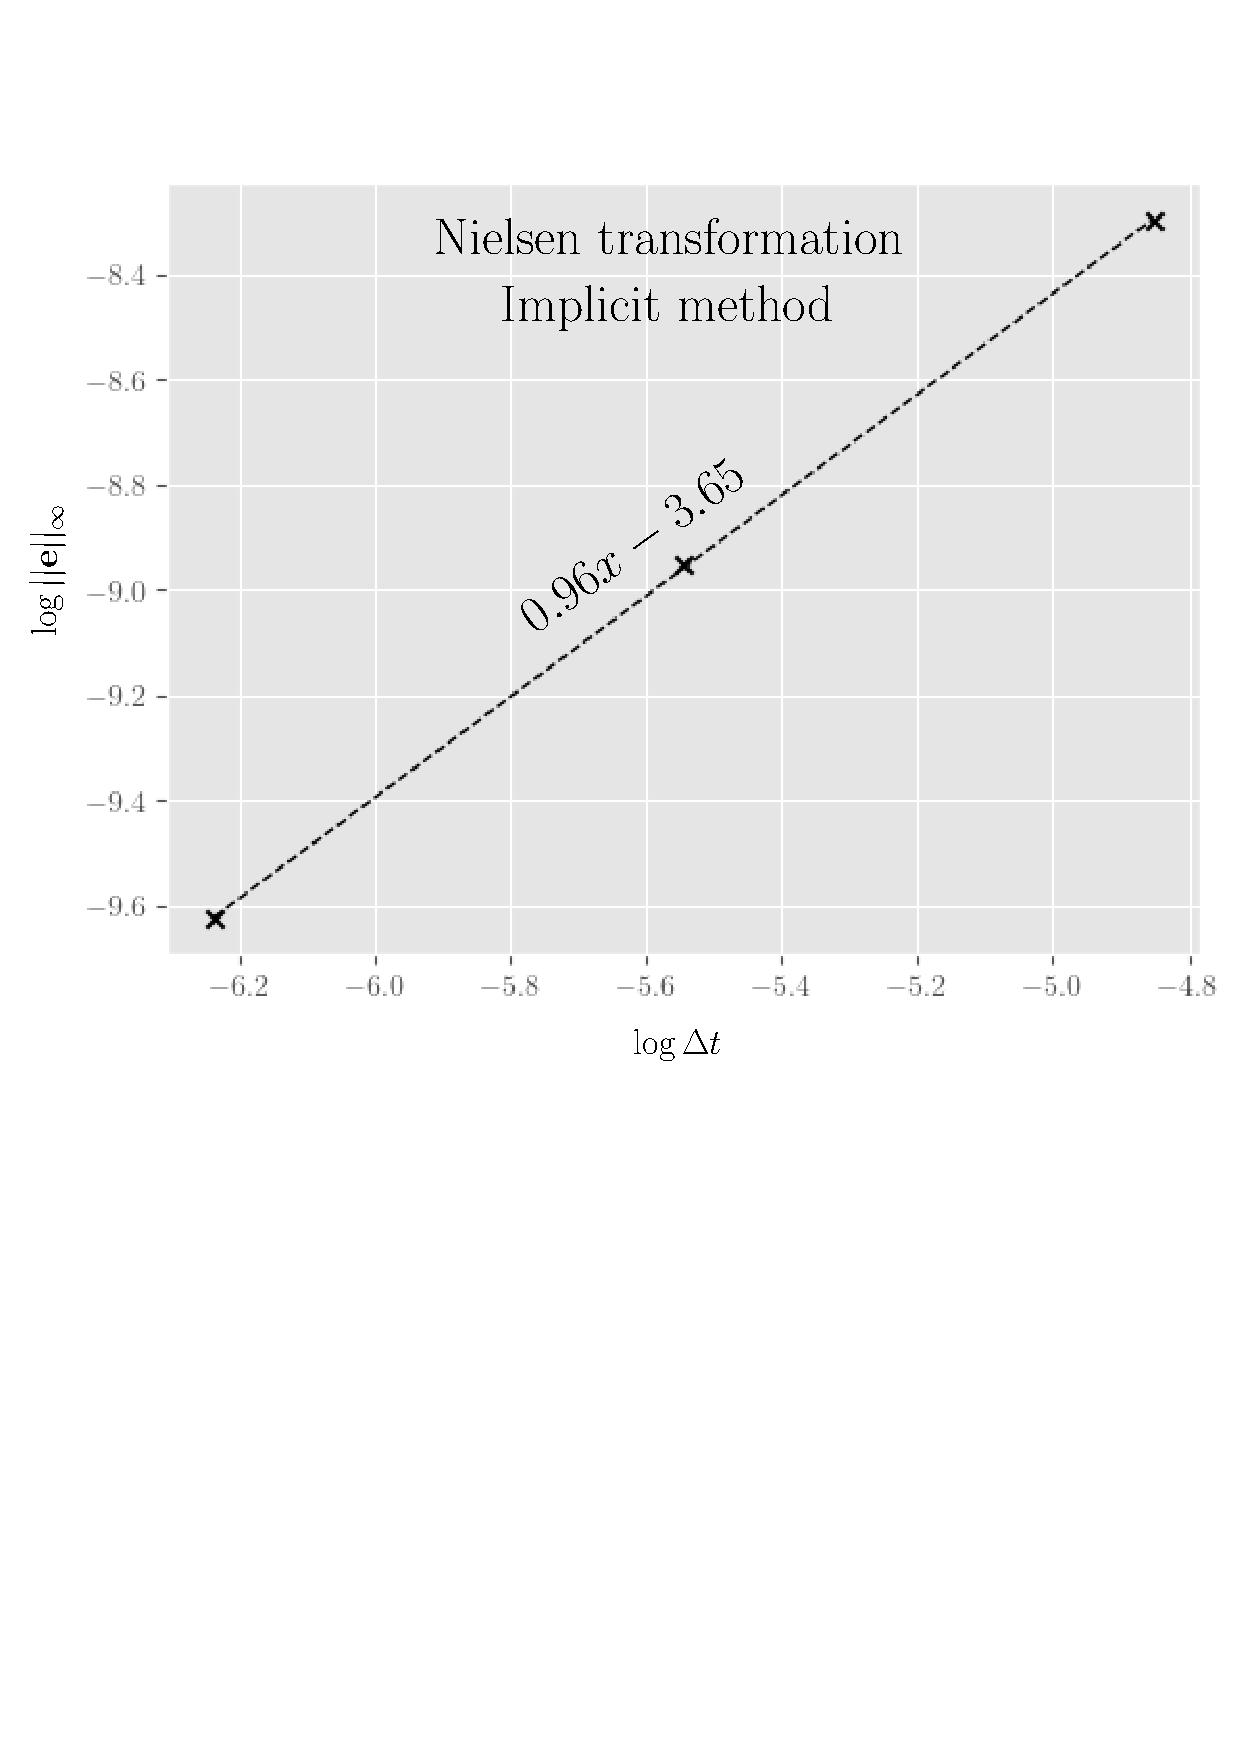
\includegraphics[width=\textwidth]{chapters/chapter3/ConvergenceTimeImplicitNielsen.pdf}
    \caption{$\Delta{t}=2^{-7},2^{-8},\dots,2^{-10}$}
    \caption*{$\Delta{x}=2^{-5}$}
  \end{subfigure}
  \caption{Convergence analysis for the explicit and implicit method for the Nielsen transformation.}
  \label{fig:finitedifferencesschemes:numericaresults:nielsen_convergence analysis}
\end{figure}

\begin{figure}[tbp]
  \centering
  \begin{subfigure}{0.4\textwidth}
    \centering
    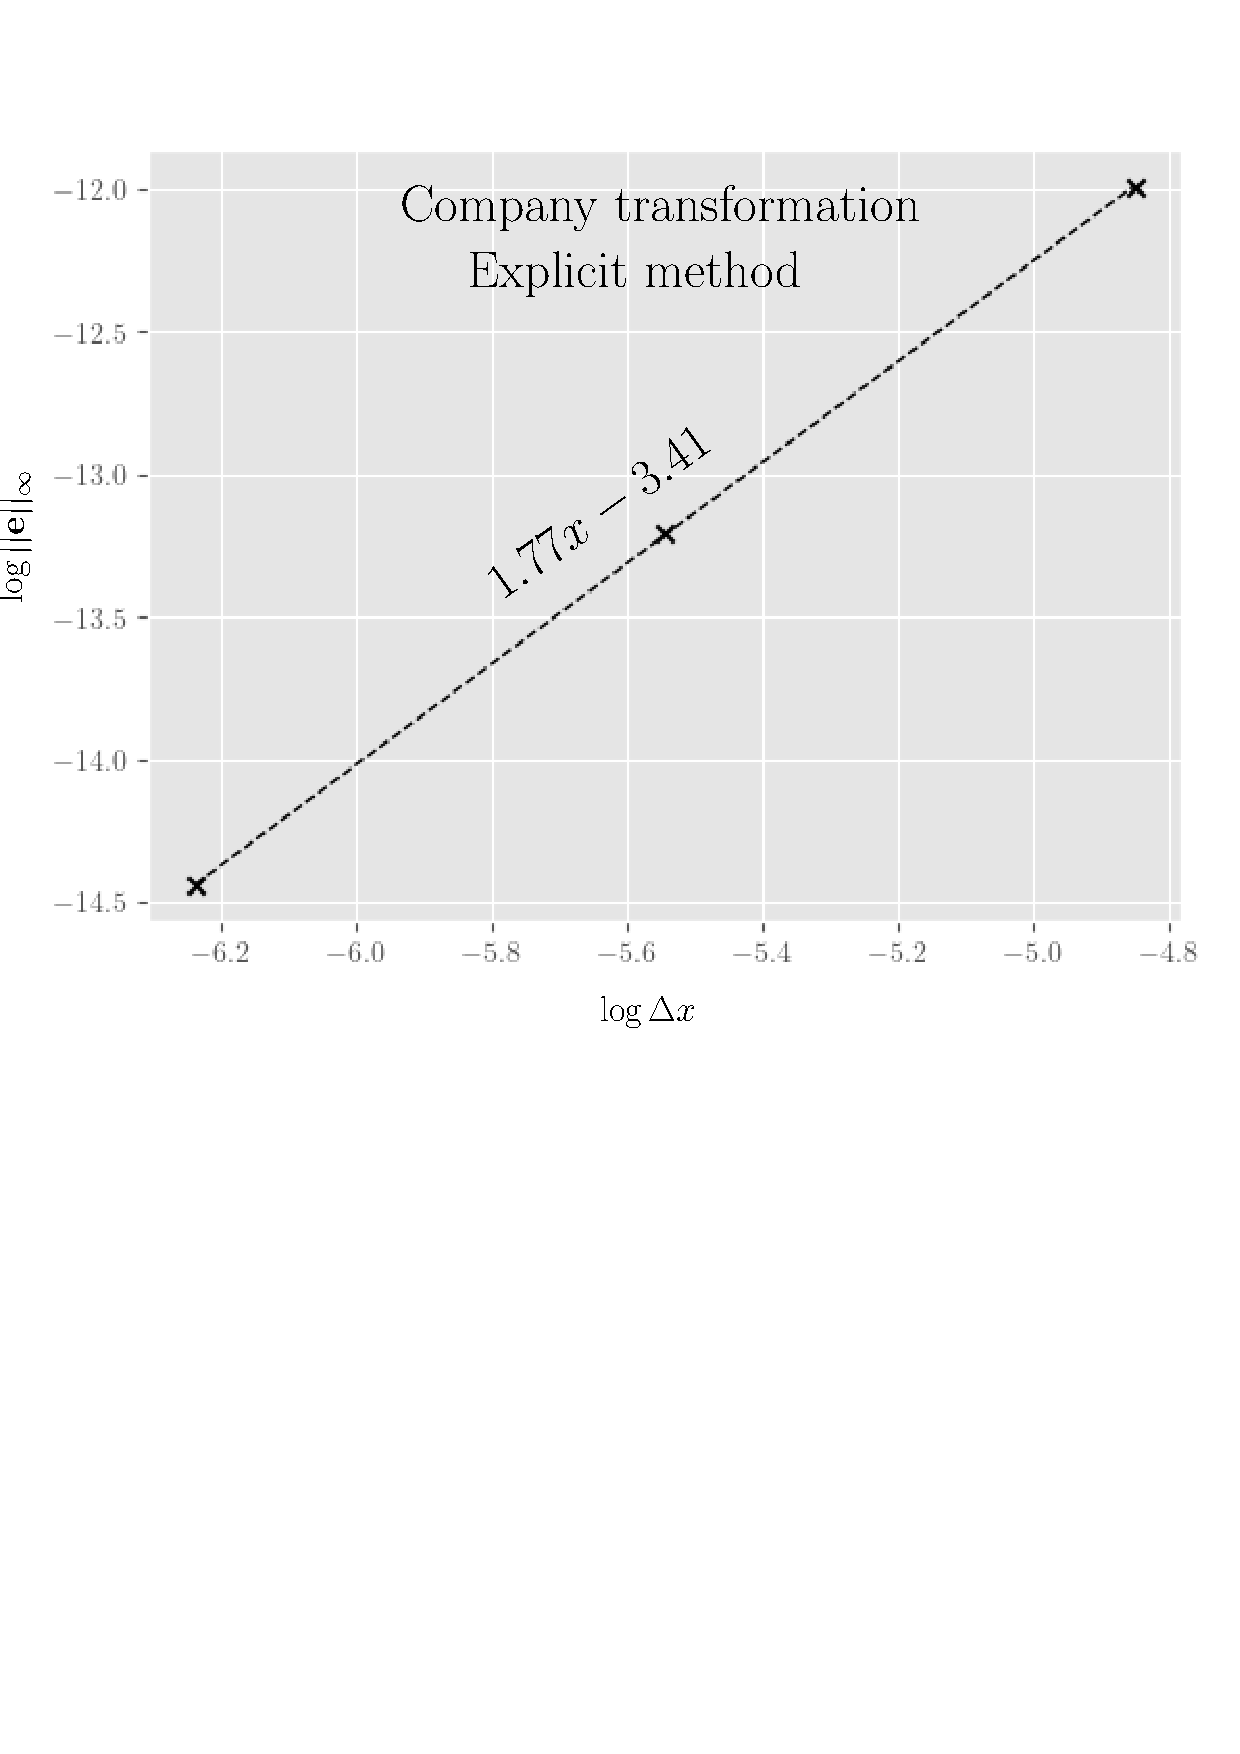
\includegraphics[width=\textwidth]{chapters/chapter3/ConvergenceSpaceExplicitCompany.pdf}
    \caption{$\Delta{x}=2^{-7},\dots,2^{-10}$}
    \caption*{$\Delta{t}=2^{-21}$}
    \label{fig:finitedifferencesschemes:numericaresults:company_explicit_space}
  \end{subfigure}
  \hspace{0.5cm}
  \begin{subfigure}{0.4\textwidth}
    \centering
    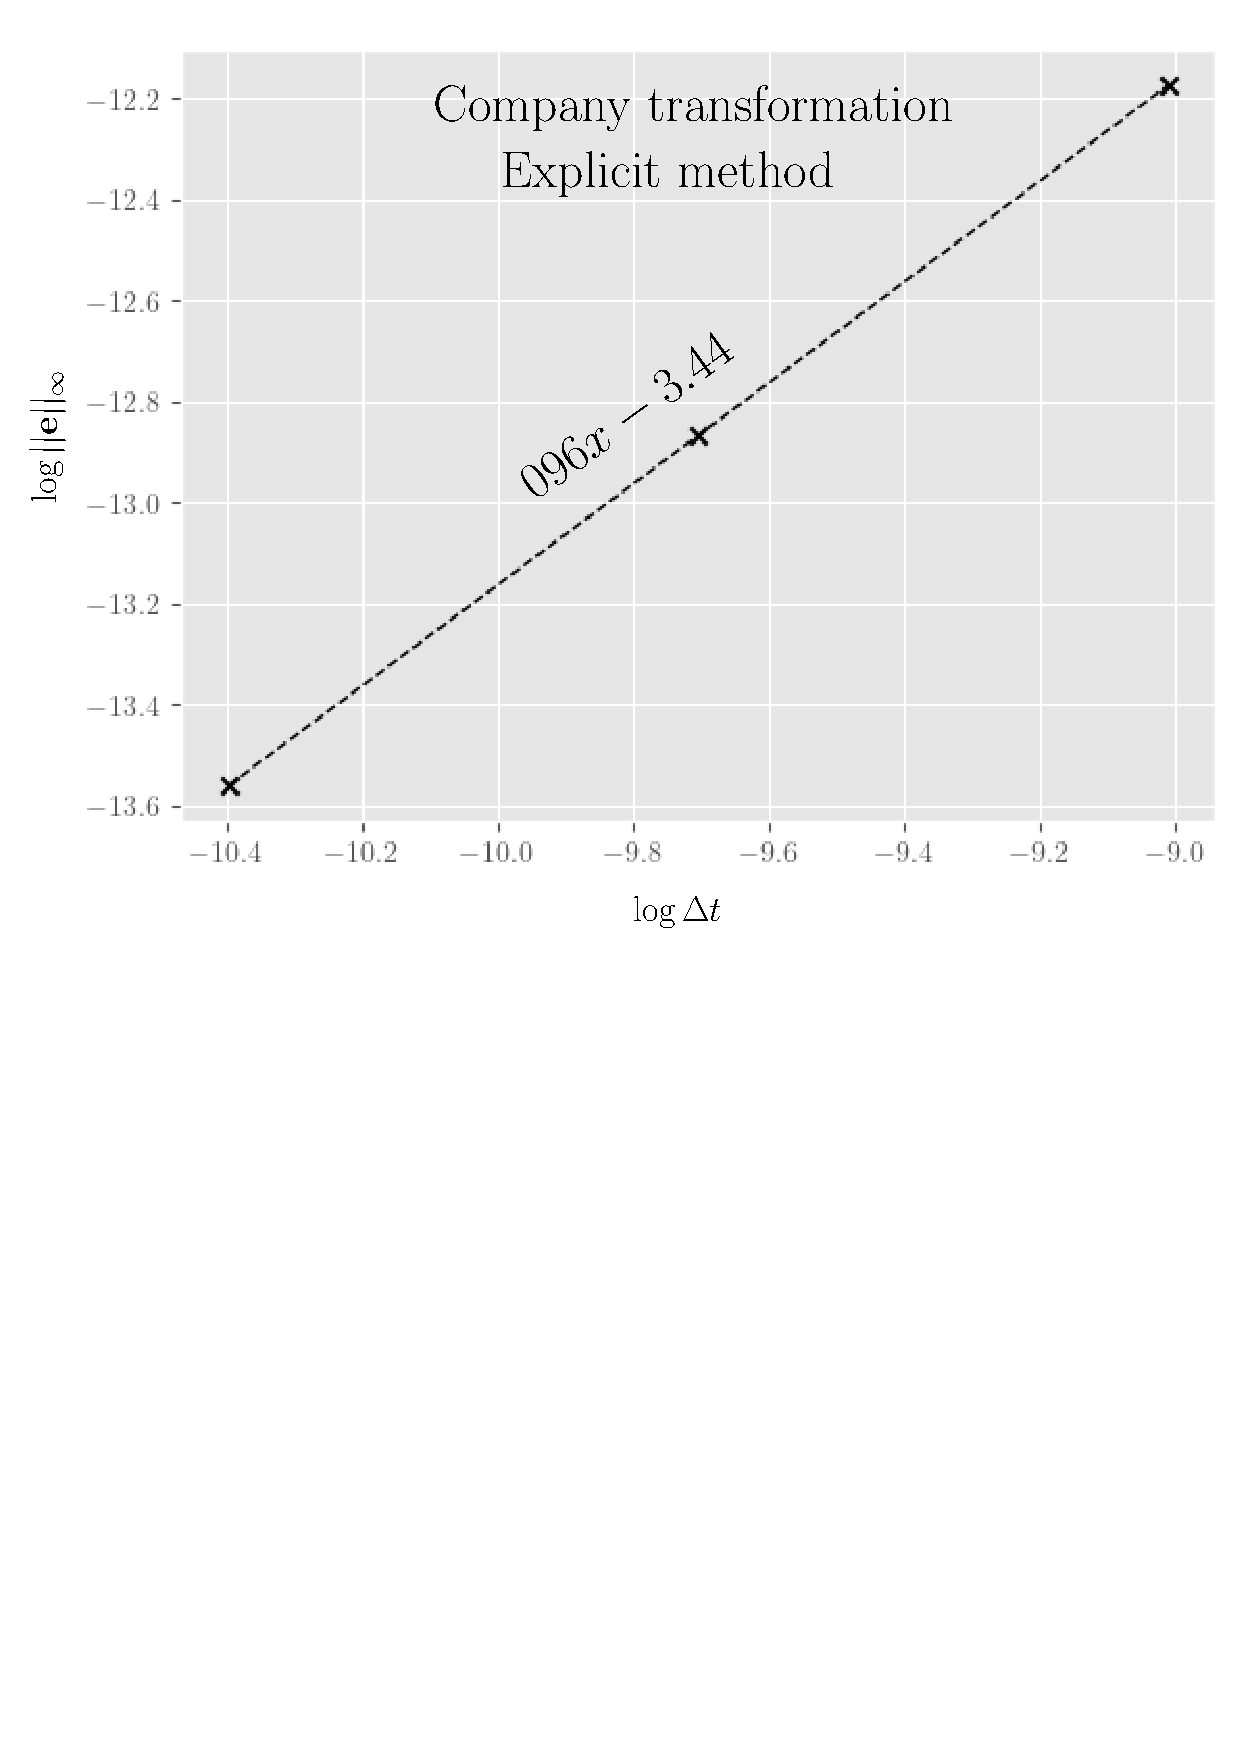
\includegraphics[width=\textwidth]{chapters/chapter3/ConvergenceTimeExplicitCompany.pdf}
    \caption{$\Delta{t}=2^{-15},2^{-17},\dots,2^{-21}$}
    \caption*{$\Delta{x}=2^{-7}$}
    \label{fig:finitedifferencesschemes:numericaresults:company_explicit_time}
  \end{subfigure}
  \caption{Convergence analysis for the explicit method for the Company transformation.}
  \label{fig:finitedifferencesschemes:numericaresults:company_convergence analysis}
\end{figure}
% \section{Numerical results}


For the setup of the experiments, we utilize the binomial option pricing model \cite{cox_1979}

We realized numerous testings to validate the correct functionality of our implementation. As Merton \cite{merton_1973} showed, pricing American call options without dividends is equivalent to solve the price of European options. Therefore, the most natural test to conduct is to price American call options without dividends ($\delta=0$) using our implementation and compare the results to the one obtain using the Black-Scholes formula for  \cite{merton_1973}. 

For the following experiments, we use the following set of parameters.
\begin{equation}
    \label{eq:numericaresults:parameters_set_1}
    K = 1, \quad T = 1, \quad r=0.2, \quad \sigma=0.2, \quad \delta = 0 
\end{equation}

Moreover, using the same set of parameters as in \eqref{eq:numericaresults:parameters_set_1}, we tested each scheme for the case of put options. For the setup of the experiments, we priced a put option using the binomial model \cite{cox_1979} with parameters \eqref{eq:numericaresults:parameters_set_1}. Then, we proceed to compute the RSME error 

\begin{equation}
    \label{eq:numericaresults:rsme}
    \text{RSME} := \bigg(\sum_{i}{(V_{\text{BOPM}} - \hat{V}_i)^2}\bigg)^{1/2}
\end{equation}

where $V^{\text{BM}}_i$ is the price produced by the binomial model, and $\hat{V}_i$ is the price produced by our numerical method. In Tables \ref{tab:rsme_explicit_nielsen_transformation} and \ref{tab:rsme_explicit_company_transformation} contain the results obtained for Nielsen and Company transformation, respectively, for $\Delta{x}=1/8, 1/16,\dots,1/128$ and $\Delta{t}=\Delta{x}^2$

% Please add the following required packages to your document preamble:
% \usepackage{booktabs}
\begin{table}[H]
    \centering
    \begin{tabular}{@{}ccccccc@{}}
    \toprule
    \textbf{Asset price} & \textbf{BOPM} & 0.125    & 0.0625   & 0.03125  & 0.015625 & 0.0078125 \\ \midrule
    0.8                  & 0.200000      & 0.200000 & 0.200000 & 0.200000 & 0.200000 & 0.200000  \\
    1.0                  & 0.048167      & 0.046048 & 0.047748 & 0.048176 & 0.048160 & 0.048155  \\
    1.2                  & 0.008666      & 0.008661 & 0.008638 & 0.008705 & 0.008674 & 0.008662  \\
    1.4                  & 0.001285      & 0.001467 & 0.001369 & 0.001313 & 0.001292 & 0.001286  \\
    1.6                  & 0.000167      & 0.000237 & 0.000196 & 0.000176 & 0.000170 & 0.000168  \\
    1.8                  & 0.000020      & 0.000038 & 0.000027 & 0.000022 & 0.000021 & 0.000020  \\
    2.0                  & 0.000002      & 0.000006 & 0.000004 & 0.000003 & 0.000002 & 0.000002  \\
                         & \textbf{RMSE} & 0.000080 & 0.000016 & 0.000002 & 0.00000  & 0.000000  \\ \bottomrule
    \end{tabular}
    \caption{\label{tab:rsme_explicit_nielsen_transformation}RSME error produced by the explicit scheme for the Nielsen transformation for $\Delta{t}=1/8,1/16,\dots,1/128$ and $\Delta{t}=\Delta{x}^2/2$.}
\end{table}

% Please add the following required packages to your document preamble:
% \usepackage{booktabs}
\begin{table}[H]
    \centering
    \begin{tabular}{@{}ccccccc@{}}
    \toprule
    \textbf{Asset price} & \textbf{BOPM} & 0.125    & 0.0625   & 0.03125  & 0.015625 & 0.0078125 \\ \midrule
    0.8                  & 0.200000      & 0.200000 & 0.200000 & 0.200000 & 0.200000 & 0.200000  \\
    1.0                  & 0.048167      & 0.049286 & 0.049274 & 0.048465 & 0.048256 & 0.048174  \\
    1.2                  & 0.008666      & 0.010736 & 0.009108 & 0.008829 & 0.008686 & 0.008667  \\
    1.4                  & 0.001285      & 0.001950 & 0.001501 & 0.001349 & 0.001295 & 0.001287  \\
    1.6                  & 0.000167      & 0.000354 & 0.000224 & 0.000185 & 0.000172 & 0.000168  \\
    1.8                  & 0.000020      & 0.000076 & 0.000035 & 0.000024 & 0.000021 & 0.000020  \\
    2.0                  & 0.000002      & 0.000017 & 0.000006 & 0.000003 & 0.000003 & 0.000002  \\
    & \textbf{RSME} & 0.000092 & 0.000045 & 0.000013 & 0.000003 & 0.00000   \\ \bottomrule
    \end{tabular}
    \caption{\label{tab:rsme_explicit_company_transformation}RSME error produced by the explicit scheme for Company transformation for $\Delta{t}=1/8,1/16,\dots,1/128$ and $\Delta{t}=\Delta{x}^2/2$.}
\end{table}

% Please add the following required packages to your document preamble:
% \usepackage{booktabs}
\begin{table}[H]
    \centering
    \begin{tabular}{@{}ccccccc@{}}
    \toprule
    \textbf{Asset price} & \textbf{BOPM}        & 0.125      & 0.0625     & 0.03125    & 0.015625   & 0.0078125  \\ \midrule
    0.8                  & 0.200000             & 0.224810   & 0.227045   & 0.200000   & 0.200000   & 0.200000   \\
    1.0                  & 0.048167             & 0.156141   & 0.159308   & 0.080886   & 0.053942   & 0.048944   \\
    1.2                  & 0.008666             & 0.114815   & 0.117140   & 0.041319   & 0.013783   & 0.009290   \\
    1.4                  & 0.001285             & 0.080638   & 0.081485   & 0.023604   & 0.003694   & 0.001519   \\
    1.6                  & 0.000167             & 0.047914   & 0.048026   & 0.014269   & 0.001085   & 0.000229   \\
    1.8                  & 0.000020             & 0.019130   & 0.020665   & 0.008591   & 0.000353   & 0.000033   \\
    2.0                  & 0.000002             & 0.000022   & 0.003408   & 0.004695   & 0.000125   & 0.000005   \\
                         & \textbf{Asset price} & 0.06812077 & 0.06970396 & 0.02045601 & 0.00307761 & 0.00038755 \\ \bottomrule
    \end{tabular}
    \caption{RSME error produced by the implicit scheme for the Nielsen transformation for $\Delta{x}=\Delta{t}=1/8,1/16,\dots,1/128$.}
\end{table}

% Please add the following required packages to your document preamble:
% \usepackage{booktabs}
\begin{table}[H]
    \begin{tabular}{@{}ccccccc@{}}
        \toprule
        \textbf{Asset price} & \textbf{BOPM} & 0.125    & 0.0625   & 0.03125  & 0.015625 & 0.0078125 \\ \midrule
        0.8                  & 0.200000      & 0.200000 & 0.200000 & 0.200000 & 0.200000 & 0.200000  \\
        1.0                  & 0.048155      & 0.046048 & 0.047748 & 0.048176 & 0.048160 & 0.048155  \\
        1.2                  & 0.008662      & 0.008661 & 0.008638 & 0.008705 & 0.008674 & 0.008662  \\
        1.4                  & 0.001286      & 0.001467 & 0.001369 & 0.001313 & 0.001292 & 0.001286  \\
        1.6                  & 0.000168      & 0.000237 & 0.000196 & 0.000176 & 0.000170 & 0.000168  \\
        1.8                  & 0.000020      & 0.000038 & 0.000027 & 0.000022 & 0.000021 & 0.000020  \\
        2.0                  & 0.000002      & 0.000006 & 0.000004 & 0.000003 & 0.000002 & 0.000002  \\
                             & \textbf{RMSE} & 0.000081 & 0.000017 & 0.000002 & 0.000000 & 0.000000  \\ \bottomrule
    \end{tabular}
\end{table}

% Please add the following required packages to your document preamble:
% \usepackage{booktabs}
\begin{table}[H]
    \begin{tabular}{@{}ccccccc@{}}
        \toprule
        \textbf{Asset price} & \textbf{BOPM} & 0.125    & 0.0625   & 0.03125  & 0.015625 & 0.0078125 \\ \midrule
        0.8                  & 0.200000      & 0.224810 & 0.227045 & 0.200000 & 0.200000 & 0.200000  \\
        1.0                  & 0.048180      & 0.156141 & 0.159308 & 0.080886 & 0.053942 & 0.048944  \\
        1.2                  & 0.008661      & 0.114815 & 0.117140 & 0.041319 & 0.013783 & 0.009290  \\
        1.4                  & 0.001283      & 0.080638 & 0.081485 & 0.023604 & 0.003694 & 0.001519  \\
        1.6                  & 0.000167      & 0.047914 & 0.048026 & 0.014269 & 0.001085 & 0.000229  \\
        1.8                  & 0.000020      & 0.019130 & 0.020665 & 0.008591 & 0.000353 & 0.000033  \\
        2.0                  & 0.000002      & 0.000022 & 0.003408 & 0.004695 & 0.000125 & 0.000005  \\
                             & \textbf{RMSE} & 0.068119 & 0.069703 & 0.020455 & 0.003076 & 0.000385  \\ \bottomrule
    \end{tabular}
\end{table}

% Please add the following required packages to your document preamble:
% \usepackage{booktabs}
\begin{table}[H]
    \begin{tabular}{@{}ccccccc@{}}
        \toprule
        \textbf{Asset price} & \textbf{BOPM} & 0.125    & 0.0625   & 0.03125  & 0.015625 & 0.0078125 \\ \midrule
        0.8                  & 0.200000      & 0.200000 & 0.200000 & 0.200000 & 0.200000 & 0.200000  \\
        1.0                  & 0.048180      & 0.054188 & 0.053469 & 0.052440 & 0.052340 & 0.052259  \\
        1.2                  & 0.008661      & 0.012658 & 0.010936 & 0.010331 & 0.010294 & 0.010271  \\
        1.4                  & 0.001283      & 0.002423 & 0.001855 & 0.001694 & 0.001650 & 0.001640  \\
        1.6                  & 0.000167      & 0.000462 & 0.000292 & 0.000250 & 0.000234 & 0.000229  \\
        1.8                  & 0.000020      & 0.000107 & 0.000048 & 0.000034 & 0.000030 & 0.000029  \\
        2.0                  & 0.000002      & 0.000028 & 0.000009 & 0.000005 & 0.000004 & 0.000004  \\
                             & \textbf{RMSE} & 0.002763 & 0.002187 & 0.001737 & 0.001695 & 0.001663  \\ \bottomrule
    \end{tabular}
\end{table}

% Please add the following required packages to your document preamble:
% \usepackage{booktabs}
\begin{table}[H]
    \begin{tabular}{@{}lllllll@{}}
        \toprule
        \textbf{Asset Price} & \textbf{BOPM} & 0.125    & 0.0625   & 0.03125  & 0.015625 & 0.0078125 \\ \midrule
        0.8                  & 0.170000      & 0.170000 & 0.170000 & 0.170000 & 0.170000 & 0.170000  \\
        1.0                  & 0.037785      & 0.038365 & 0.038260 & 0.037619 & 0.037754 & 0.037773  \\
        1.2                  & 0.006576      & 0.007278 & 0.006645 & 0.006602 & 0.006573 & 0.006573  \\
        1.4                  & 0.000953      & 0.001132 & 0.001013 & 0.000969 & 0.000953 & 0.000952  \\
        1.6                  & 0.000122      & 0.000185 & 0.000142 & 0.000128 & 0.000124 & 0.000123  \\
        1.8                  & 0.000015      & 0.000038 & 0.000021 & 0.000016 & 0.000015 & 0.000015  \\
        2.0                  & 0.000002      & 0.000008 & 0.000003 & 0.000002 & 0.000002 & 0.000002  \\
                             & \textbf{RMSE} & 0.000035 & 0.000018 & 0.000006 & 0.000001 & 0.000000  \\ \bottomrule
    \end{tabular}
\end{table}
\section{Linear complementary problem}
\subsection{Overview}
A linear complementary problem (LCP) is an optimization problem in which the goal is to solve a system of linear equations subject to a set of complementary conditions. More formally, given the matrix $\mathbf{A}\in\mathbb{R}^{d \times d}$ and the vector $\mathbf{b}\in\mathbb{R}^{d}$, we have to find the vectors $\mathbf{v}\in\mathbb{R}^{d}$ and $\mathbf{w}\in\mathbb{R}^{d}$ such as
\begin{align*}
  \mathbf{A}\mathbf{v} - \mathbf{w} = \mathbf{b}
\end{align*}
subject to the complementary conditions 
\begin{align*}
  v_i &\ge 0 \qquad \text{for $i = 1,\dots,d$} \\
  w_i &\ge 0 \qquad \text{for $i = 1,\dots,d$} \\
  \mathbf{v}^{T}\mathbf{w} &= 0
\end{align*}
Note that the complementary conditions require that either $v_i=0$ or $w_i=0$. As you will see later, the pricing problem for American options can be reformulated as a linear complementary problem. But first, let us reconsider what the Black-Scholes model tells about American options. First, that the value $V(S,t)$ is bounded from below by the payoff function 
\begin{align*}
  V(S, t) - H(S, t) \ge 0 \qquad \text{for all $(S,t)$}
\end{align*}
Secondly, the value function can be divided in two complementary regions: the exercise region \eqref{eq:blackscholes:preliminaries:exercise_region} where  
\begin{align}
  \label{eq:lcp:overview:value_in_continuation_region}
  &V(S, t) - H(S, t) > 0 \qquad \text{for $(S,t) \in \mathcal{C}$}
\end{align}
the continuation region \eqref{eq:blackscholes:preliminaries:continuation_region} where 
\begin{align}
  \label{eq:lcp:overview:value_in_exercise_region}
  &V(S, t) - H(S, t) = 0 \qquad \text{for $(S,t) \in \mathcal{S}$}
\end{align}
Finally, value function $V(S,t)$ is the solution to the Black-Scholes PDE  within the continuation region
\begin{align*}
    \frac{\partial{V}}{\partial{t}} + \mathcal{L}_{\text{BS}}(V) = 0 \qquad \text{for $(S,t) \in \mathcal{C}$}
\end{align*}
where $\mathcal{L}_{\text{BS}}(\cdot)$ is the linear parabolic operator \eqref{eq:blackscholes:preliminaries:linear_parabolic_operator} applied to the function $V(S,t)$. Now, let us consider what happens to the Black-Scholes PDE in the exercise region. From equation \eqref{eq:lcp:overview:value_in_exercise_region}, we know that $V(S,t)=H(S,t)$. Hence, by plugin $H(S,t)$ in the Black-Scholes PDE, we obtain the Black-Scholes PDE inequality
\begin{align}
    \label{eq:lcp:overview:blackscholes_in_exercise_region}
    \frac{\partial{V}}{\partial{t}} + \mathcal{L}_{\text{BS}} \le 0 \qquad \text{for $(S,t) \in \mathcal{S}$}
\end{align}
By grouping \eqref{eq:lcp:overview:value_in_continuation_region}, \eqref{eq:lcp:overview:value_in_exercise_region}, \eqref{eq:lcp:overview:blackscholes_in_exercise_region}, we form the system of variational inequalities
\begin{align}
  \begin{cases}
    \big[\frac{\partial V}{\partial \tau} - \mathcal{L}_{\text{BS}}(V)\big] \cdot [V(S,T-\tau) - H(S,T-\tau)] = 0 & \text{for all $(S,\tau)$} \\
    V(S, T-\tau) - H(S, T-\tau) \ge 0 & \text{for all $(S,\tau) \ $}\\
    \frac{\partial V}{\partial \tau} - \mathcal{L}_{\text{BS}}(V) \ge 0 &  \text{for all $(S,\tau)$}\\
    V(S, T -\tau) = H(S, T - \tau) \\  
  \end{cases}
  \label{eq:lcp:overview:variational_inequalities}
\end{align}
where $\tau := T - t$. The benefit of the variational inequalities is that there is no explicit dependence on the optimal exercise price defined in \eqref{eq:blackscholes:preliminaries:optimal_exercise_boundary}. Also, note that we rewrote the Black-Scholes PDE forward in time by introducing the transformation $\tau = T - t$ deliberately so that the variational inequalities' formulation looks similar in structure to the LCP problem defined at the beginning of this section. But before elaborating more about the relationship between the variational inequalities and LCP problems, we introduce the transformations
\begin{align}
\label{eq:lcp:overview:heat_diffusion_domain_transformation}
S = Ke^x, \quad t = T - \dfrac{2\tau}{\sigma^2},\quad h(x,\tau) := e^{(\alpha x + \beta \tau)}\dfrac{H(S,t)}{K}, \quad v(x, \tau) := V(S, t) =: Ke^{-(\alpha x + \beta \tau)}y(x, \tau)
\end{align}
where
\begin{align}
  \label{eq:lcp:overview:heat_diffusion_domain_transformation_2}
  q &:= \dfrac{2r}{\sigma^2}, \quad q_{\delta} := \dfrac{2(r-\delta)}{\sigma^2}, \quad \alpha := \dfrac{1}{2}(q_{\delta} - 1) \quad \beta := \dfrac{1}{4}(q_{\delta} - 1)^2 + q 
\end{align}
so that the Black-Scholes PDE inequality \eqref{eq:lcp:overview:blackscholes_in_exercise_region} transforms to the heat diffusion inequality
\begin{align}
  \label{eq:lcp:overview:heat_diffusion_equation_PDE}
  \dfrac{\partial{y}}{\partial{\tau}} - \dfrac{\partial^2{y}}{\partial{x^2}} &\le 0 \qquad \text{for $x \in \mathbb{R}$ and $\tau\in(0, \sigma^2T/2]$}
\end{align}
where $y\in C^{2,1}\big(\mathbb{R}\times[0, \sigma^2T/2]\big)$ have boundary conditions
\begin{align}
  \lim_{x\rightarrow-\infty}y(x, \tau) &= \lim_{x\rightarrow-\infty}h(0, \tau)  = 0 \\
  \lim_{x\rightarrow\infty}y(x, \tau) &= \lim_{x\rightarrow\infty}h(0, \tau) = 0
\end{align}
and initial condition 
\begin{align}
  y(x, 0) = h(x, 0)
\end{align}
Although we might solve \eqref{eq:lcp:overview:variational_inequalities} without transforming the problem, Dewynne et al.\cite{dewynne_howison_rupf_wilmott_1993} and Seydel\cite{seydel_2009} suggest that transformation to the heat diffusion equation \eqref{eq:lcp:overview:heat_diffusion_equation_PDE} introduces desirable numerical properties when applying finite difference schemes. By applying transformation \eqref{eq:lcp:overview:heat_diffusion_domain_transformation}, the system \eqref{eq:lcp:overview:variational_inequalities} becomes
\begin{align}
  \begin{cases}
    \bigg[\dfrac{\partial{y}}{\partial{\tau}} - \dfrac{\partial^2{y}}{\partial{x^2}}\bigg] \cdot [y(x, \tau) - h(x, \tau)] = 0 & \text{for all $(x,\tau)$} \\
    y(x, \tau) - h(x, \tau) \ge 0 & \text{for all $(x, \tau)$}\\
    \dfrac{\partial{y}}{\partial{\tau}} - \dfrac{\partial^2{y}}{\partial{x^2}} \ge 0 &  \text{for all $(x, \tau)$}\\
    y(x, 0) = h(x, 0) \\  
  \end{cases}
  \label{eq:lcp:overview:variational_inequalities_heat_equation}
\end{align}
Now that we have expressed the system of variational inequalities using the heat discussion equation, we proceed to apply the finite difference scheme framework presented in section \ref{sec:finitedifferencesschemes}. Specifically, we want to approximate $y(x, \tau)$ at each node within the grid 
\begin{align}
  \mathcal{G} &:= \{(x_i, \tau_n): (i, n) \in \{0, \dots, M+1\} \times \{0, \dots, N+1\}\}\\
  \label{eq:lcp:overview:grid_2}
  x_i &:= x_{\text{min}} + i\Delta{x} \quad \text{for $i = 0,\dots, M+1$} \\
  \tau_n &:= t_{\text{min}} + i{\Delta{\tau}} \quad \text{for $i = 0,\dots, N+1$} \\
  \Delta{x} &:= \dfrac{x_{\text{max}} - x_{\text{min}}}{M+1} \\ 
  \Delta{t} &:= \dfrac{t_{\text{max}} - t_{\text{min}}}{N+1}
\end{align}
where $x_{\text{min}}$ is set sufficiently small value, $x_{\text{max}}$ to a sufficiently large value, $\tau_{\text{min}}$ to 0 and $\tau_{\text{max}}$ to $\dfrac{\sigma^2}{2}T$. Recall that we presented explicit and implicit schemes for approximating the PDE \eqref{eq:blackscholes:frontfixingmethod:nielsen:american_options_pde} in section \ref{sec:finitedifferencesschemes}. Analogously, we present explicit and implicit schemes for the heat diffusion equation
\begin{align}
  \label{eq:lcp:overview:explicit_scheme}
  \dfrac{y^{n+1}_{i} - y^{n}_{i}}{\Delta \tau} =& \dfrac{y^{n}_{i-1} - 2y^{n}_{i} + y^{n}_{i+1}}{(\Delta x)^2}\\
  \label{eq:lcp:overview:implicit_scheme}
  \dfrac{y^{n+1}_{i} - y^{n}_{i}}{\Delta \tau} =& \dfrac{y^{n+1}_{i-1} - 2y^{n+1}_{i} + y^{n+1}_{i+1}}{(\Delta x)^2}
\end{align}
for $i=1,\dots,M$ and $n=0\dots,N$. Note that contrary to \eqref{eq:blackscholes:frontfixingmethod:nielsen:american_options_pde}, the heat equation is written forward in time. Therefore, the explicit scheme correspond to equation \eqref{eq:lcp:overview:explicit_scheme}, and the implicit scheme to equation \eqref{eq:lcp:overview:implicit_scheme}. In addition, we introduce the Crank-Nicholson scheme\cite{epperson_2013}\cite{seydel_2009} for equation \eqref{eq:lcp:overview:heat_diffusion_equation_PDE} as 
\begin{equation}
  \label{eq:lcp:overview:crank_nicholson}
  \dfrac{y^{n+1}_{i} - y^{n}_{i}}{\Delta \tau} = \dfrac{1}{2}\bigg(\dfrac{y^{n}_{i-1} - 2y^{n}_{i} + y^{n}_{i+1}}{(\Delta x)^2} + \dfrac{y^{n+1}_{i-1} - 2y^{n+1}_{i} + y^{n+1}_{i+1}}{(\Delta x)^2}\bigg)
\end{equation}
for $i=1,\dots,M$ and $n=0\dots,N$. Epperson\cite{epperson_2013} and Seydel\cite{seydel_2009} showed that the Crank-Nicholson scheme is $O(\Delta{x}^2 + \Delta{t}^2)$.
\begin{figure}[H]
  \label{fig:lcp:thetamethod:stencil}
  \centering
  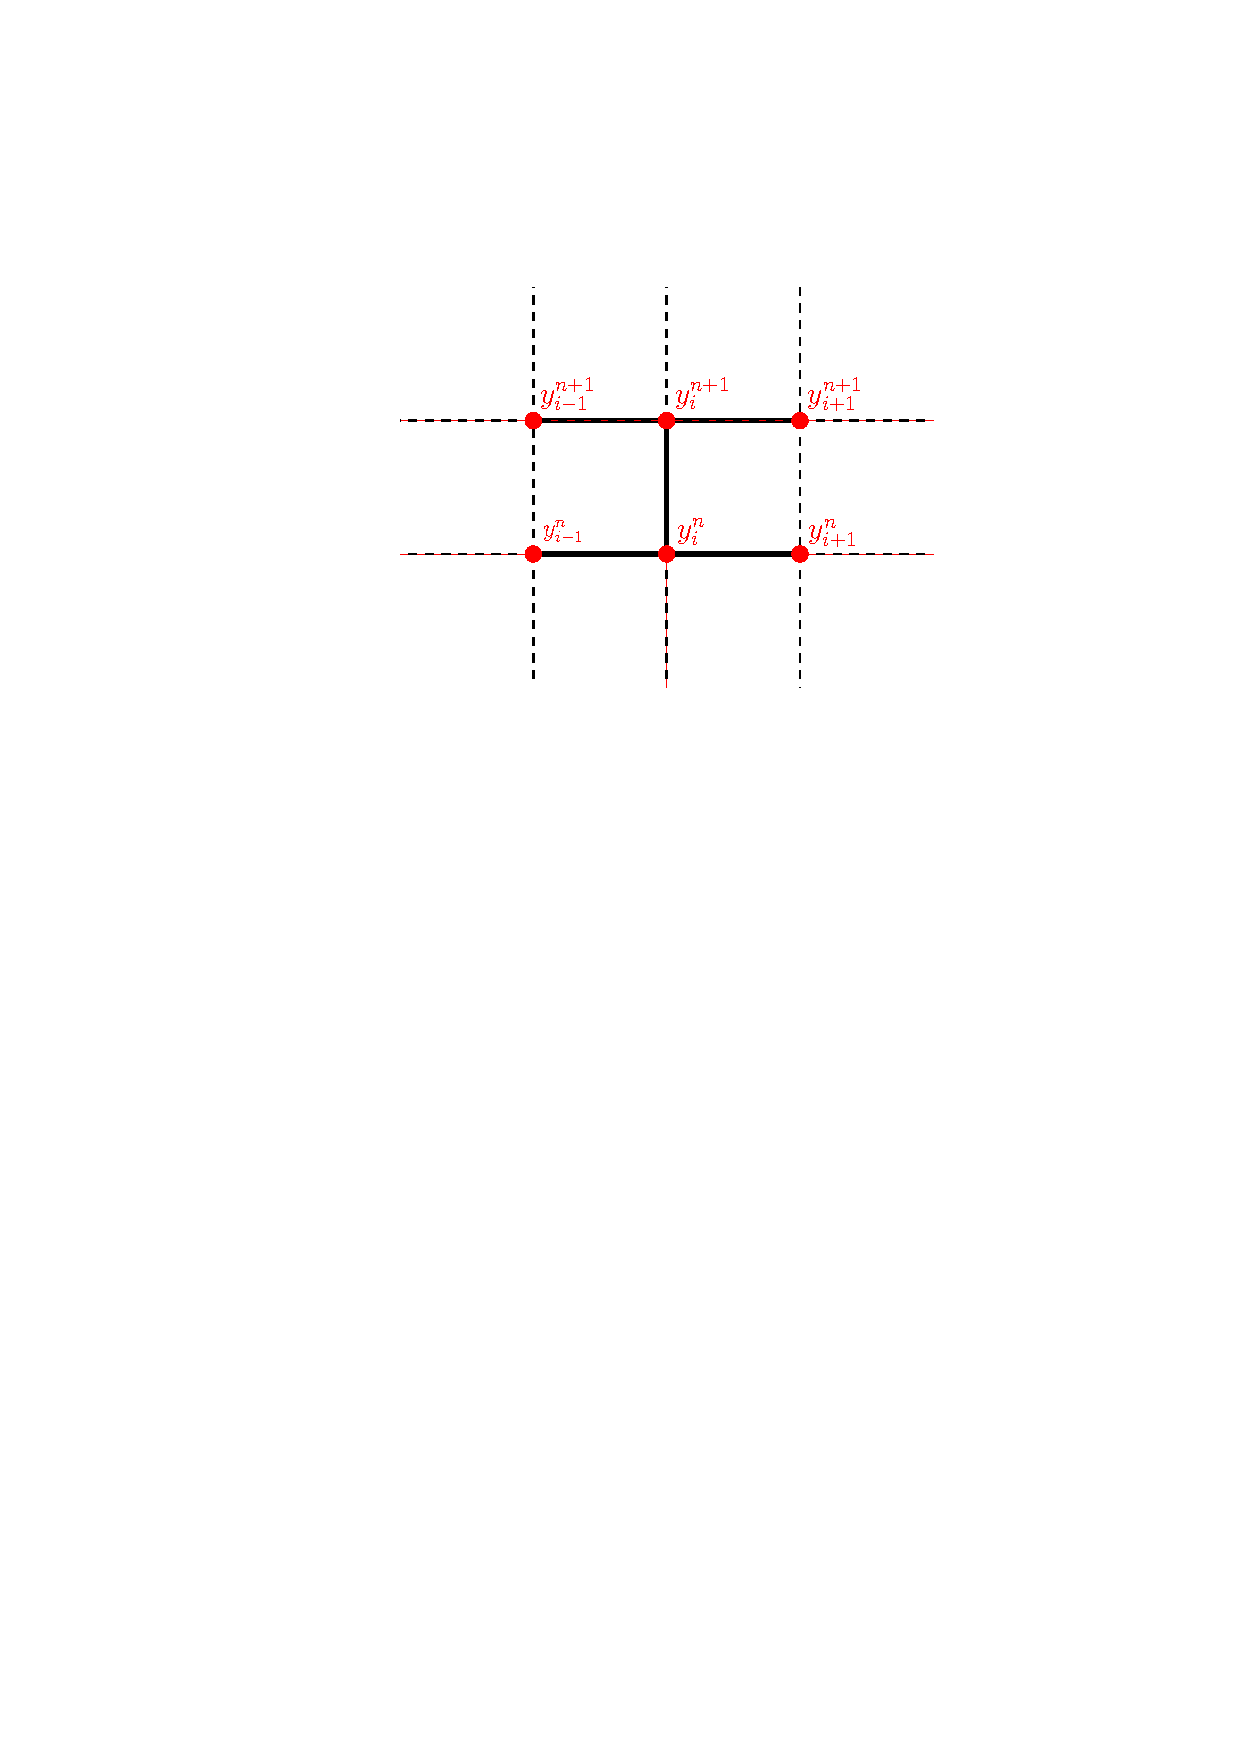
\includegraphics[scale=0.75]{chapters/chapter5/CrankNicholsonStencil.pdf}
  \caption{Stencil diagram for the Crank-Nicholson scheme.}
\end{figure} 
We can generalize \eqref{eq:lcp:overview:explicit_scheme}, \eqref{eq:lcp:overview:implicit_scheme}, and \eqref{eq:lcp:overview:crank_nicholson} using a parametrized scheme called the theta method 
\begin{equation}
  \label{eq:lcp:overview:theta_method}
  \dfrac{y^{n+1}_{i} - y^{n}_{i}}{\Delta \tau} = (1-\theta)\dfrac{y^{n}_{i-1} - 2y^{n}_{i} + y^{n}_{i+1}}{(\Delta x)^2} + \theta\dfrac{y^{n+1}_{i-1} - 2y^{n+1}_{i} + y^{n+1}_{i+1}}{(\Delta x)^2}
\end{equation}
for $i = 1,\dots,M$, and $n = 0,\dots,N$. The parameter $\theta\in[0,1]$ controls what scheme to use. The scheme defaults to the explicit method when $\theta=0$, to the implicit method when $\theta=1$, to the Crank-Nicholson when $\theta=1/2$. Next, we rearrange equation \eqref{eq:lcp:overview:theta_method} as
\begin{equation}
  \label{eq:lcp:thetamethod:finitedifference_approximation_2}
  y^{n+1}_{i} - \lambda\theta(y^{n+1}_{i-1} - 2y^{n+1}_{i} + y^{n+1}_{i+1}) =  y^{n}_{i} + (1-\theta)\lambda(y^{n}_{i-1} - 2y^{n}_{i} + y^{n}_{i+1})
\end{equation}
for $i = 1,\dots,M$, $n = 0,\dots,N$, and $\lambda=\Delta{t}/\Delta{x}^2$. Moreover, let us define vectors $\hat{\mathbf{b}}^n\in\mathbb{R}^{M}$, $\mathbf{y}^{n+1}\in\mathbb{R}^{M}$ and $\mathbf{h}^n\in\mathbb{R}^{M}$ as
\begin{align}
  \label{eq:lcp:thetamethod:b_hat}
  \hat{\mathbf{b}}^{n} :=& \begin{bmatrix}
    \hat{b}^{n}_1, \dots, \hat{b}^{n}_{M}
  \end{bmatrix}^{\textbf{T}}\\
  \mathbf{y}^{n+1} :=& \begin{bmatrix}
    y^{n+1}_1, \dots, y^{n+1}_{M}
  \end{bmatrix}^{\textbf{T}}\\
  \label{eq:lcp:thetamethod:h_vector}
  \mathbf{h}^{n+1} :=& \begin{bmatrix}
    h(x_1, \tau_{n+1}), \dots, h(x_M, \tau_{n+1})
  \end{bmatrix}^{\textbf{T}}
\end{align}
where 
\begin{equation}
  \hat{b}^{n}_i := y^{n}_{i} + (1-\theta)\lambda(y^{n}_{i-1} - 2y^{n}_{i} + y^{n}_{i+1})
\end{equation}
for $i = 1,\dots,M$, and $n = 0,\dots,N$. Finally, we define the matrix $\mathbf{A}\in\mathbb{R}^{M \times M}$ as
\begin{align}
  \label{eq:lcp:overview:theta_matrix}
  \mathbf{A} :=& \begin{bmatrix}
    1+2\lambda\theta & -\lambda\theta & & 0 \\ 
   -\lambda\theta & \ddots & \ddots \\
      & \ddots & \ddots & \ddots \\
    0 & & \ddots & \ddots & \\
  \end{bmatrix} 
\end{align}
Hence, using vectors $\hat{\mathbf{b}}^n\in\mathbb{R}^{M}$, $\mathbf{y}^{n+1}\in\mathbb{R}^{M}$ and $\mathbf{h}^n\in\mathbb{R}^{M}$, and the matrix $\mathbf{A}\in\mathbb{R}^{M \times M}$, we could rewrite the system of variational inequalities \eqref{eq:lcp:overview:variational_inequalities_heat_equation}using the finite difference scheme proposed as
\begin{align}
  \label{eq:lcp:overview:variational_inequalities_fd}
  \begin{cases}
    (\mathbf{A}\mathbf{y}^{n+1} - \hat{\mathbf{b}}^{n})^{\text{T}}(\mathbf{y}^{n+1}- \mathbf{h}^{n+1}) = 0\\
    \mathbf{A}\mathbf{y}^{n+1} - \hat{\mathbf{b}}^{n} \ge 0\\
    \mathbf{y}^{n+1}- \mathbf{h}^{n+1} \ge 0\\
    \mathbf{y}^{0} = \mathbf{h}^{0}
  \end{cases}
\end{align}
for $n=0,\dots,N$. Moreover, \eqref{eq:lcp:overview:variational_inequalities_fd} can be formulated as the iterative method
\begin{algorithm}[H]
  \caption{Iterative method for variational inequalities.}\label{alg:lcp:overview:variational_inequalities_iterative_method}
  \begin{algorithmic}
  \State $\mathbf{y}^{0} = \mathbf{h}^{0}$
  \For{$n = 0,\dots,N$} 
  \State Find $\mathbf{y}^{n+1}$ such as 
  \State $\qquad (\mathbf{A}\mathbf{y}^{n+1} - \hat{\mathbf{b}}^{n})^{\text{T}}(\mathbf{y}^{n+1}- \mathbf{h}^{n+1}) = 0$
  \State $\qquad \mathbf{A}\mathbf{y}^{n+1} - \hat{\mathbf{b}}^{n} \ge 0$
  \State $\qquad \mathbf{y}^{n+1}- \mathbf{h}^{n+1} \ge 0$
  \EndFor
\end{algorithmic}
\end{algorithm}
\newpage
Finally, by defining $\mathbf{v} := \mathbf{y}^{n+1} - \mathbf{h}^{n+1}$,  $\mathbf{w} := \mathbf{A}\mathbf{y}^{n+1} - \hat{\mathbf{b}}^{n}$, $\mathbf{b} := \hat{\mathbf{b}}^n - \mathbf{A}\mathbf{h}^{n+1}$. The iterative \ method becomes
\begin{algorithm}[H]
  \caption{Iterative method for LCP.}\label{alg:lcp:overview:lcp_iterative_method}
  \begin{algorithmic}
  \For{$n = 0,\dots,N$} 
  \State Given $\mathbf{A}\mathbf{v} - \mathbf{w} = \mathbf{b}$, find $\mathbf{v}$ and $\mathbf{w}$ such as 
  \State $\qquad \mathbf{v} \ge 0$
  \State $\qquad \mathbf{w} \ge 0$
  \State $\qquad \mathbf{v}^{\text{T}}\mathbf{w} \ge 0$
  \EndFor
\end{algorithmic}
\end{algorithm}
Note, that solving the variational inequalities is equivalent to solve an LCP problem for $n=0,\dots,N$.
\subsection{PSOR method}
The LCP reformulation for the pricing problem requires to solve a system of linear equations subject to complementary conditions. Therefore, we consider the problem of solving the linear equation $\mathbf{A}\mathbf{x}=\mathbf{b}$ for $\mathbf{A}\in\mathbb{R}^n$, and $\mathbf{b}\in\mathbb{R}^n$. Suppose that $\mathbf{M} = \mathbf{A} + \mathbf{N}$ is a non-singular matrix. Then, the linear equation can be rewritten as
\begin{align}
  \mathbf{M}\mathbf{x}=\mathbf{N}\mathbf{x} + \mathbf{b}
\end{align}
or as 
\begin{align}
  \label{eq:lcp:psor:fix_point_equation}
  \mathbf{x} = \mathbf{B}\mathbf{x} + \mathbf{M}^{-1}\mathbf{b}
\end{align}
where $\mathbf{B} := \mathbf{M}^{-1}\mathbf{N} = \mathbf{I}-\mathbf{M}^{-1}\mathbf{A}$. Clearly, equation \eqref{eq:lcp:psor:fix_point_equation} constitute fixed-point problem\cite{epperson_2013} which leads to the iterative method
\begin{align}
  \label{eq:lcp:psor:fix_point_iterative}
  \mathbf{x}^{k} = \mathbf{B}\mathbf{x}^{k-1} + \mathbf{M}^{-1}\mathbf{b}
\end{align}
Epperson\cite{epperson_2013} showed that iterative method \eqref{eq:lcp:psor:fix_point_iterative} converges given an initial guess $\mathbf{x}^{0}$ when
\begin{align*}
  \rho(\mathbf{B}) < 1
\end{align*}
where $\rho(\mathbf{B})$ is the spectral radius of matrix $\mathbf{B}$. Different choices of matrix $\mathbf{M}$ will yield to different methods with different convergence rate. The Jacobi method defines $\mathbf{M}$ and $\mathbf{N}$ such as $\mathbf{A}=\mathbf{M}-\mathbf{N}=\mathbf{D} - (\mathbf{L} + \mathbf{U})$, yielding the iterative method
\begin{align}
  \mathbf{D}\mathbf{x}^{k} = (\mathbf{L} + \mathbf{U})\mathbf{x}^{k-1} + \mathbf{M}^{-1}\mathbf{b}
\end{align}
According to Epperson\cite{epperson_2013}, the Jacaobi method has the slowest convergence of all the other iterative methods that we could come with. Similarly, the Gauss-Seidel method is given by defining $\mathbf{M} := \mathbf{D} - \mathbf{L}$ and $\mathbf{N}:=\mathbf{U}$.
\begin{align}
  \label{eq:lcp:psor:gauss_seydel}
  (\mathbf{D} - \mathbf{L})\mathbf{x}^{k} = \mathbf{U}\mathbf{x}^{k-1} + \mathbf{M}^{-1}\mathbf{b}
\end{align}
A generalization of the Gauss-Seidel \eqref{eq:lcp:psor:gauss_seydel} method is given by is the successive over-relaxation (SOR) method. The SOR method defines $M$ and $N$ as 
\begin{align*}
  \mathbf{M} := \frac{1}{\omega}\mathbf{D} - \mathbf{L}, \qquad \mathbf{N}=\bigg(\frac{1}{\omega} -1\bigg)\mathbf{D} + \mathbf{U}
\end{align*}
where $\omega$ is the relaxation parameter. Thus, resulting in the iterative method
\begin{align}
  \label{eq:lcp:psor:sor_method}
  \bigg(\frac{1}{\omega}\mathbf{D} - \mathbf{L}\bigg)\mathbf{x}^{k} = \bigg(\bigg(\frac{1}{\omega}-1\bigg)\mathbf{D} + \mathbf{U}\bigg)\mathbf{x}^{k-1} + \mathbf{b}
\end{align}
Note that for $\omega=1$, the Gauss-Seidel \eqref{eq:lcp:psor:sor_method} method is obtained. Suppose, we want to solve $\mathbf{A}\mathbf{v}=\mathbf{b}$ for $\mathbf{A}$ given as in \eqref{eq:lcp:overview:theta_matrix}, $\mathbf{v}\in\mathbb{R}^{M}$, and $\mathbf{b}\in\mathbb{R}^{M}$. Then, a componentwise version of the \eqref{eq:lcp:psor:sor_method} is given by 
\begin{align}
  \label{eq:lcp:psor:sor_method_cwise}
  \frac{1}{\omega}(1+2\alpha)v^{k}_i = \bigg(\frac{1}{\omega}-1\bigg)(1+2\alpha)v^{k-1}_{i} + \alpha (v^{k}_{i-1} + v^{k-1}_{i+1}) + b_i
\end{align}
for $\alpha=\lambda\theta$ and $i=1,\dots,M$. Moreover, an iterative algorithm will be given as
\begin{algorithm}[H]
  \caption{SOR for the theta method.}\label{alg:lcp:overview:sor_method_theta}
  \begin{algorithmic}[1]
  \For{$k = 1,\dots$} 
  \For{$i = 1,\dots, M$}
  \State $r^{k}_{i} = (\alpha(v^{k}_{i-1} + v^{k-1}_{i+1}) + b_i)/(1+2\alpha)$ 
  \State $v^{k}_{i} = v^{k-1}_i + \omega(r^{k}_{i} - v^{k-1}_i)$
  \EndFor
  \EndFor
\end{algorithmic}
\end{algorithm}
The project SOR (PSOR) method is a slight modification of SOR method in which the positivity of $v^{k}_i$ is enforced at line number 5 of \eqref{alg:lcp:overview:sor_method_theta}.
\begin{algorithm}[H]
  \caption{PSOR for the theta method.}\label{alg:lcp:overview:psor_method_theta}
  \begin{algorithmic}[1]
  \For{$k = 1,\dots$} 
  \For{$i = 1,\dots, M$}
  \State $r^{k}_{i} = (\alpha(v^{k}_{i-1} + v^{k-1}_{i+1}) + b_i)/(1+2\alpha)$ 
  \State $v^{k}_{i} = \max\big\{0, v^{k-1}_i + \omega(r^{k}_{i} - v^{k-1}_i)\big\}$
  \EndFor
  \EndFor
\end{algorithmic}
\end{algorithm}
Moreover, Seydel et al.\cite{seydel_2009} and Dewynne et al.\cite{dewynne_howison_wilmott_howison_1995} showed that the PSOR method is equivalent to LCP algorithm \eqref{alg:lcp:overview:lcp_iterative_method}. Moreover, they also showed that the fastest convergence is given by having $\omega=1$. Putting algorithm \eqref{alg:lcp:overview:variational_inequalities_iterative_method}, \eqref{alg:lcp:overview:lcp_iterative_method} and \eqref{alg:lcp:overview:psor_method_theta} together, we have
\begin{algorithm}[H]
  \caption{Iterative method for solving heat diffusion variational inequalities.}\label{alg:lcp:psor:amer_option_solution}
  \begin{algorithmic}[1]
  \State Define $h(x,\tau)$ as in \eqref{eq:lcp:overview:heat_diffusion_domain_transformation}.
  \State Define grid as in \eqref{eq:lcp:overview:grid_2}.
  \State Set $\omega$ to 1.
  \State Set $\epsilon$ to some value closes to zero.
  \State $\mathbf{y}^{n}=h(x_i, 0)$ for $i=1,\dots,M$
  \For{$n = 0,\dots,N$} \Comment{Beginning of LCP problem}
    \State Define $\mathbf{h}^{n+1}$ as in \eqref{eq:lcp:thetamethod:b_hat}.
    \State Define $\hat{\mathbf{b}}^n$ as in \eqref{eq:lcp:thetamethod:h_vector}.
    \State $v^{0}_{i} := \max(y^{n}_i, h^{n+1}_i) \quad \text{for $i=1,\dots,M$}$\Comment{Beginning of PSOR method}
    \For{$k = 1,\dots$} 
    \For{$i = 1,\dots, M$}
    \State $r^{k}_{i} := (\alpha(v^{k}_{i-1} + v^{k-1}_{i+1}) + b_i)/(1+2\alpha)$ 
    \State $v^{k}_{i} := \max\big\{0, v^{k-1}_i + \omega(r^{k}_{i} - v^{k-1}_i)\big\}$
    \EndFor
    \If {$||\mathbf{v}^{k}-\mathbf{v}^{k-1}||_{2} \le \epsilon$}
      \State $\mathbf{v}^{\text{new}} := \mathbf{v}^{k}$
      \State Break out of the loop
    \EndIf
    \EndFor
    \State $\mathbf{y}^{n+1} :=\mathbf{v}^{k}$
  \EndFor
\end{algorithmic}
\end{algorithm}

\subsection{Numerical results}

\subsubsection{Numerical experiments}
\begin{figure}[H]
  \centering
  \begin{subfigure}{0.4\textwidth}
    \centering
    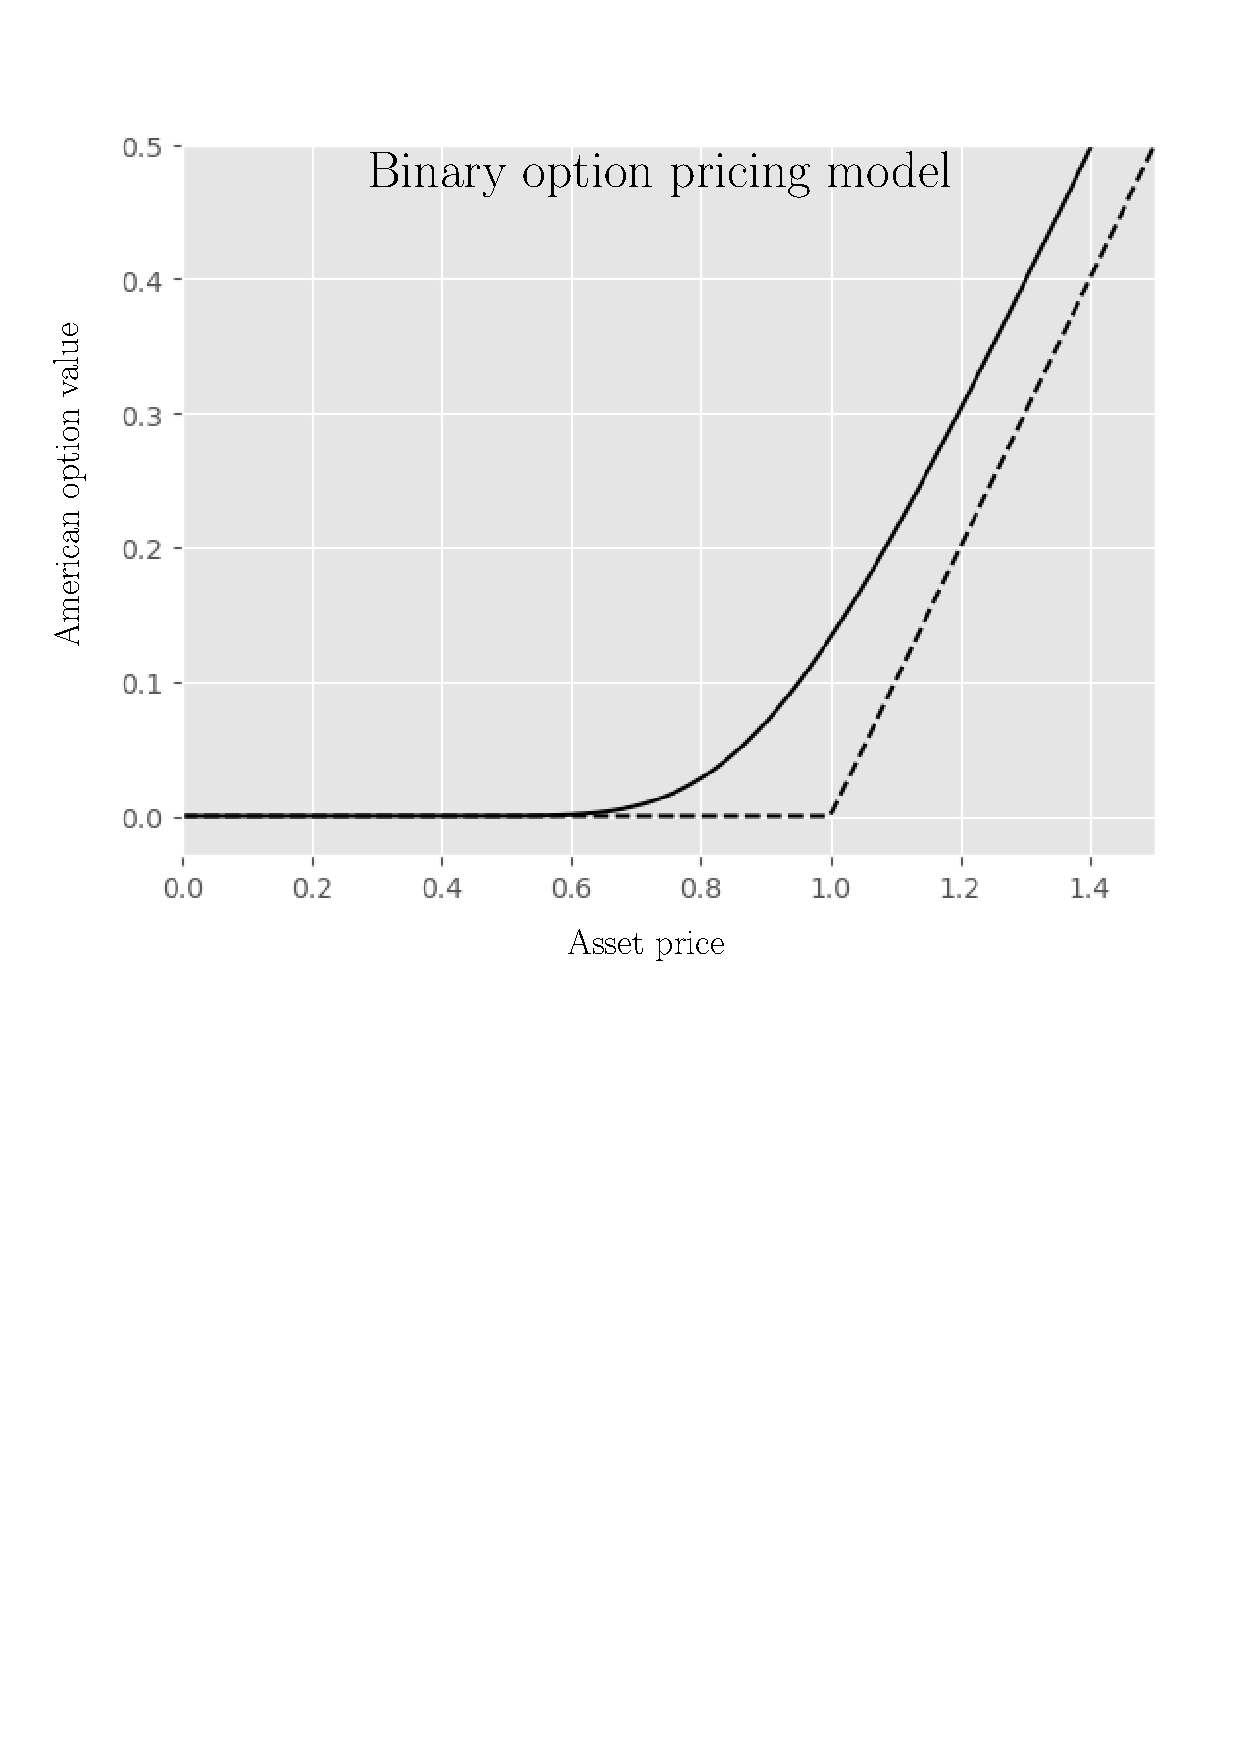
\includegraphics[width=\textwidth]{chapters/chapter3/TestCase1BOPM.pdf}
    \caption{$\text{Nodes} = 2^{500}$.}
    \label{fig:lcp:numericaresults:numericaresults:test_case_1_bopm}
  \end{subfigure}
  \hspace{0.5cm}
  \begin{subfigure}{0.4\textwidth}
    \centering
    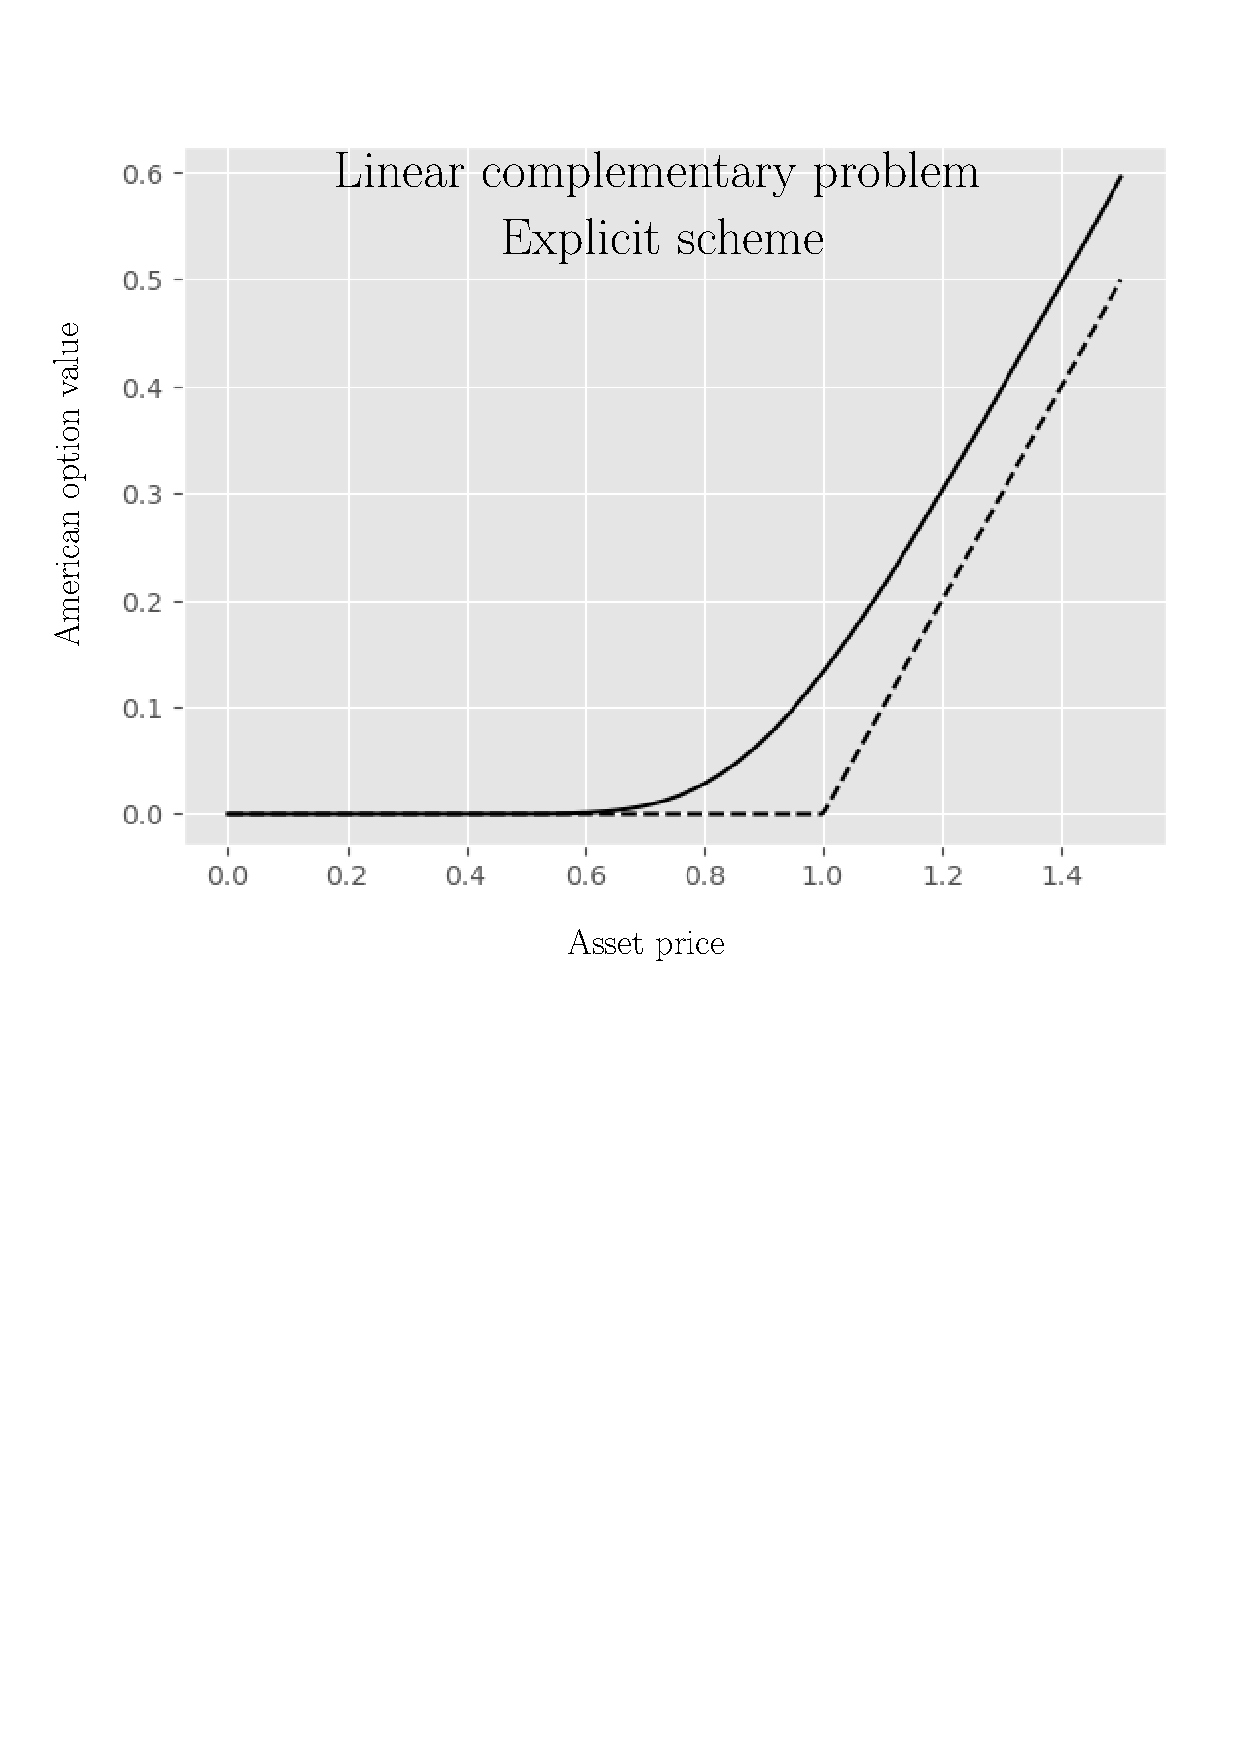
\includegraphics[width=\textwidth]{chapters/chapter5/TestCase1ExplicitLCP.pdf}
    \caption{$\Delta{x}=\expnumber{1}{-3}, \Delta{t}=0.5\times\expnumber{1}{-6}$}
    \label{fig:lcp:numericaresults:test_case_1_explicit}
  \end{subfigure}
  \begin{subfigure}{0.4\textwidth}
    \centering
    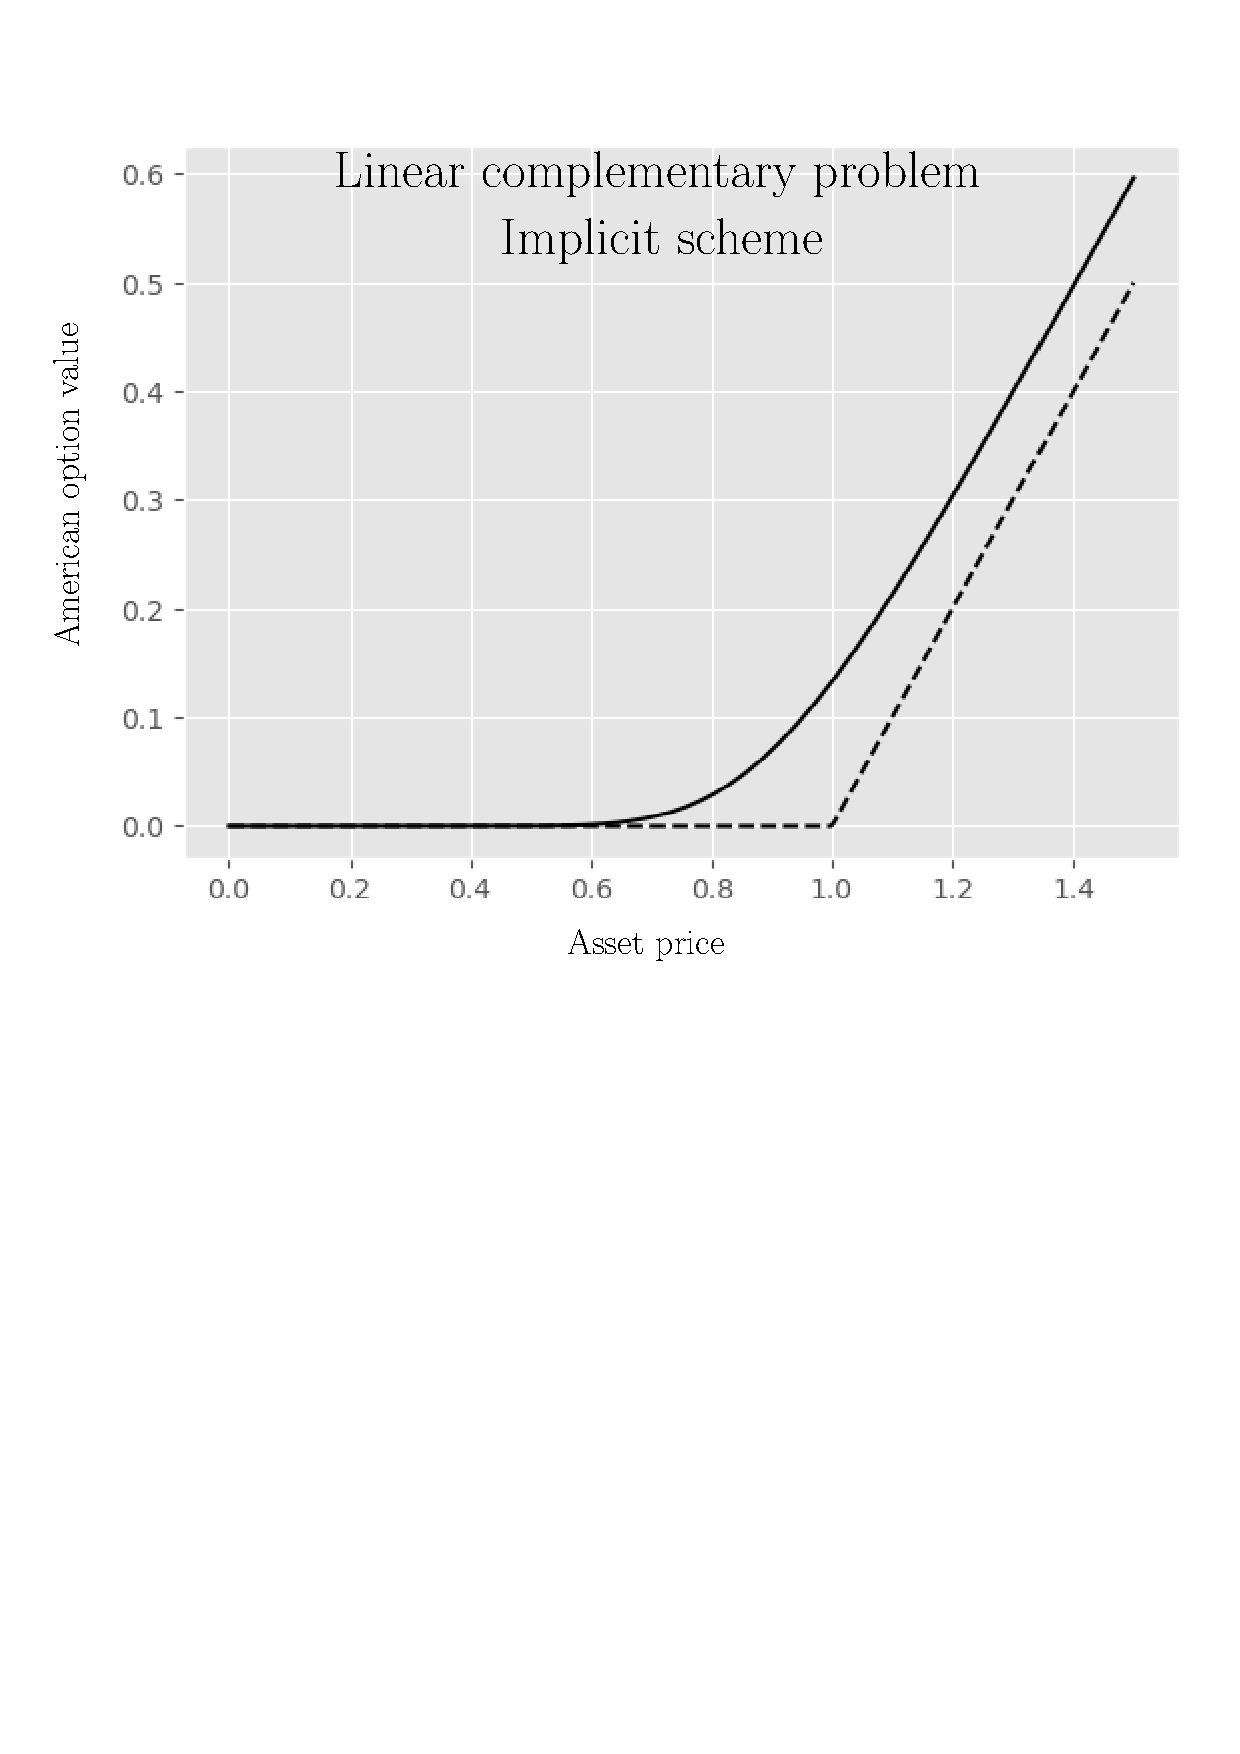
\includegraphics[width=\textwidth]{chapters/chapter5/TestCase1ImplicitLCP.pdf}
    \caption{$\Delta{x}=\expnumber{1}{-3}, \Delta{t}=0.5\times\expnumber{1}{-6}$}
    \label{fig:lcp:numericaresults:test_case_1_implicit}
  \end{subfigure}
  \hspace{0.5cm}
  \begin{subfigure}{0.4\textwidth}
    \label{fig:lcp:numericaresults:test_case_1_crank_nicholson}
    \centering
    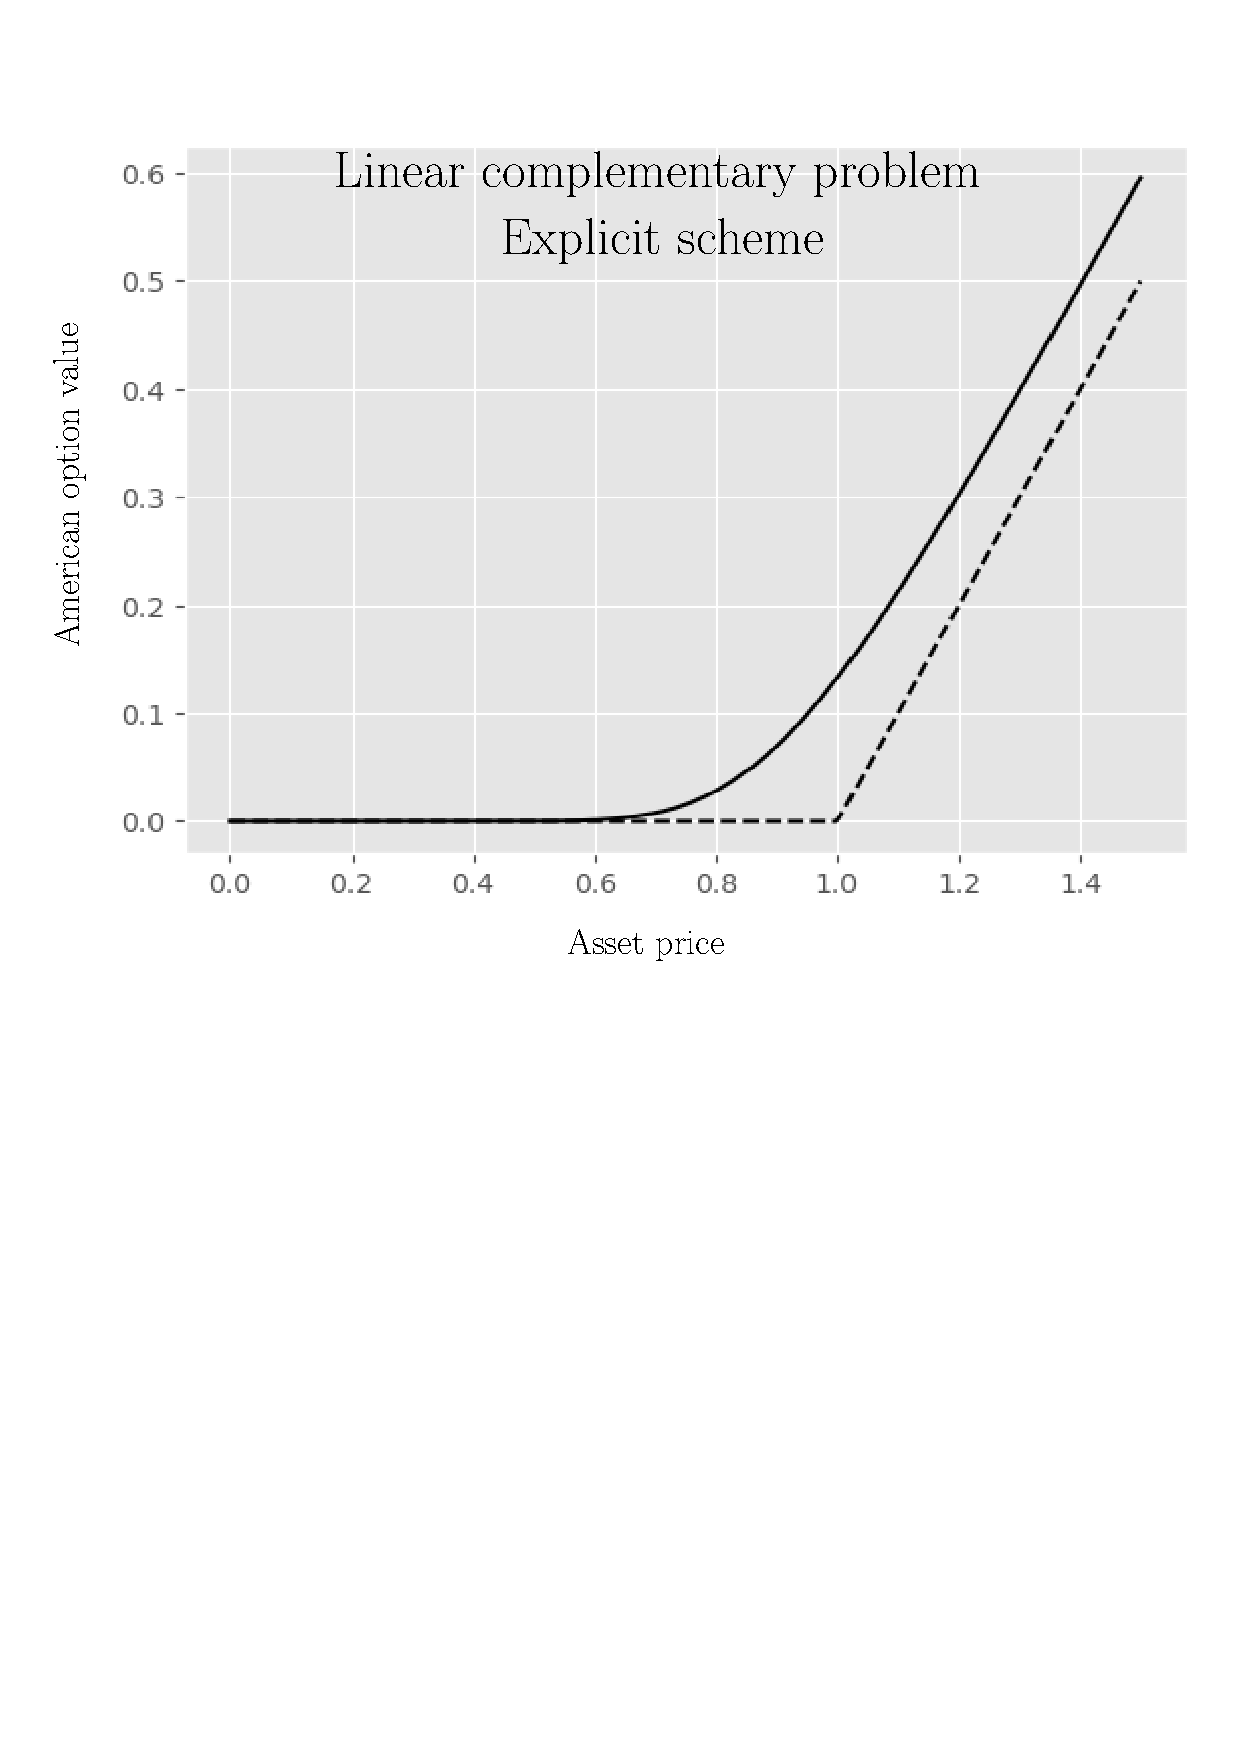
\includegraphics[width=\textwidth]{chapters/chapter5/TestCase1CrankNicholsonLCP.pdf}
    \caption{$\Delta{x}=\Delta{t}=\expnumber{1}{-3}$.}
  \end{subfigure}
  \caption{American call option value $V(S, 0)$ given parameters \eqref{eq:numericaresults:parameters_set_1}.}
  \label{fig:lcp:numericaresults:numericaresults:test_case_1}
\end{figure}
% Please add the following required packages to your document preamble:
% \usepackage{booktabs}
\begin{table}[H]
  \centering
  \begin{tabular}{@{}ccccc@{}}
  \toprule
  \textbf{Asset Price} &
    \textbf{BOPM} &
    \textbf{\begin{tabular}[c]{@{}c@{}}Explicit\\ Nielsen\end{tabular}} &
    \textbf{\begin{tabular}[c]{@{}c@{}}Implicit\\ Nielsen\end{tabular}} &
    \textbf{\begin{tabular}[c]{@{}c@{}}Explicit\\ Company\end{tabular}} \\ \midrule
  0.8 & 0.027907      & 0.028005 & 0.027907 & 0.028011 \\
  1.0 & 0.132688      & 0.132621 & 0.132688 & 0.132626 \\
  1.2 & 0.302596      & 0.302686 & 0.302596 & 0.302694 \\
  1.4 & 0.496317      & 0.496474 & 0.496317 & 0.496484 \\
  1.6 & 0.695316      & 0.695494 & 0.695316 & 0.695507 \\
  1.8 & 0.895181      & 0.895384 & 0.895181 & 0.895398 \\
      & \textbf{RMSE} & 0.000156 & 0.000826 & 0.000166 \\
      & \textbf{Time} & 5062ms   & 2168ms   & 1480ms   \\ \bottomrule
  \end{tabular}
  \caption{
  \label{tab:lcp:test_case_1}  $V(S, 0)$ call approximation given parameters \eqref{eq:numericaresults:parameters_set_1}.}
  \end{table}


\begin{figure}[tbp]
  \centering
  \begin{subfigure}{0.4\textwidth}
    \centering
    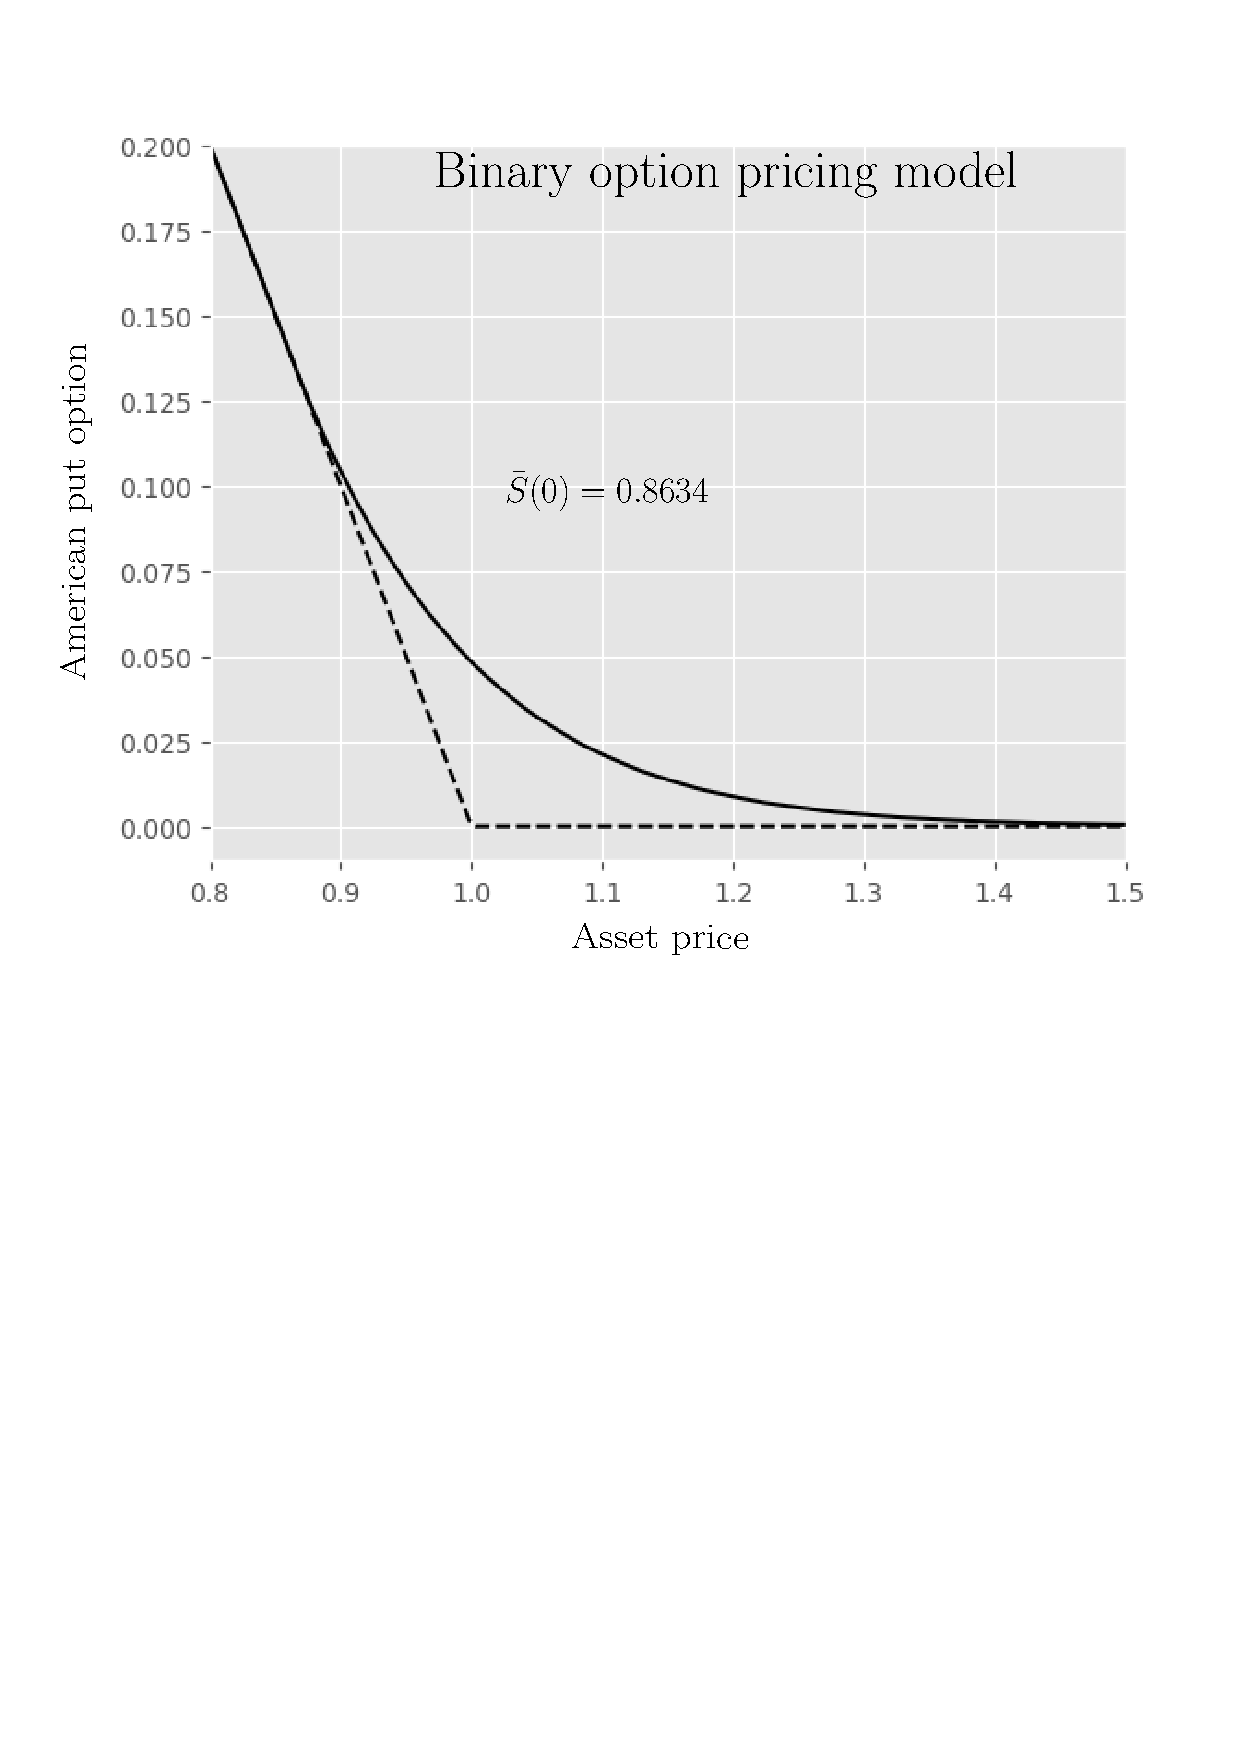
\includegraphics[width=\textwidth]{chapters/chapter5/TestCase2LcpBOPM.pdf}
    \caption{$\text{Nodes} = 2^{500}$.}
    \label{fig:lcp:numericaresults:test_case_2_bopm}
  \end{subfigure}
  \hspace{0.5cm}
  \begin{subfigure}{0.4\textwidth}
    \centering
    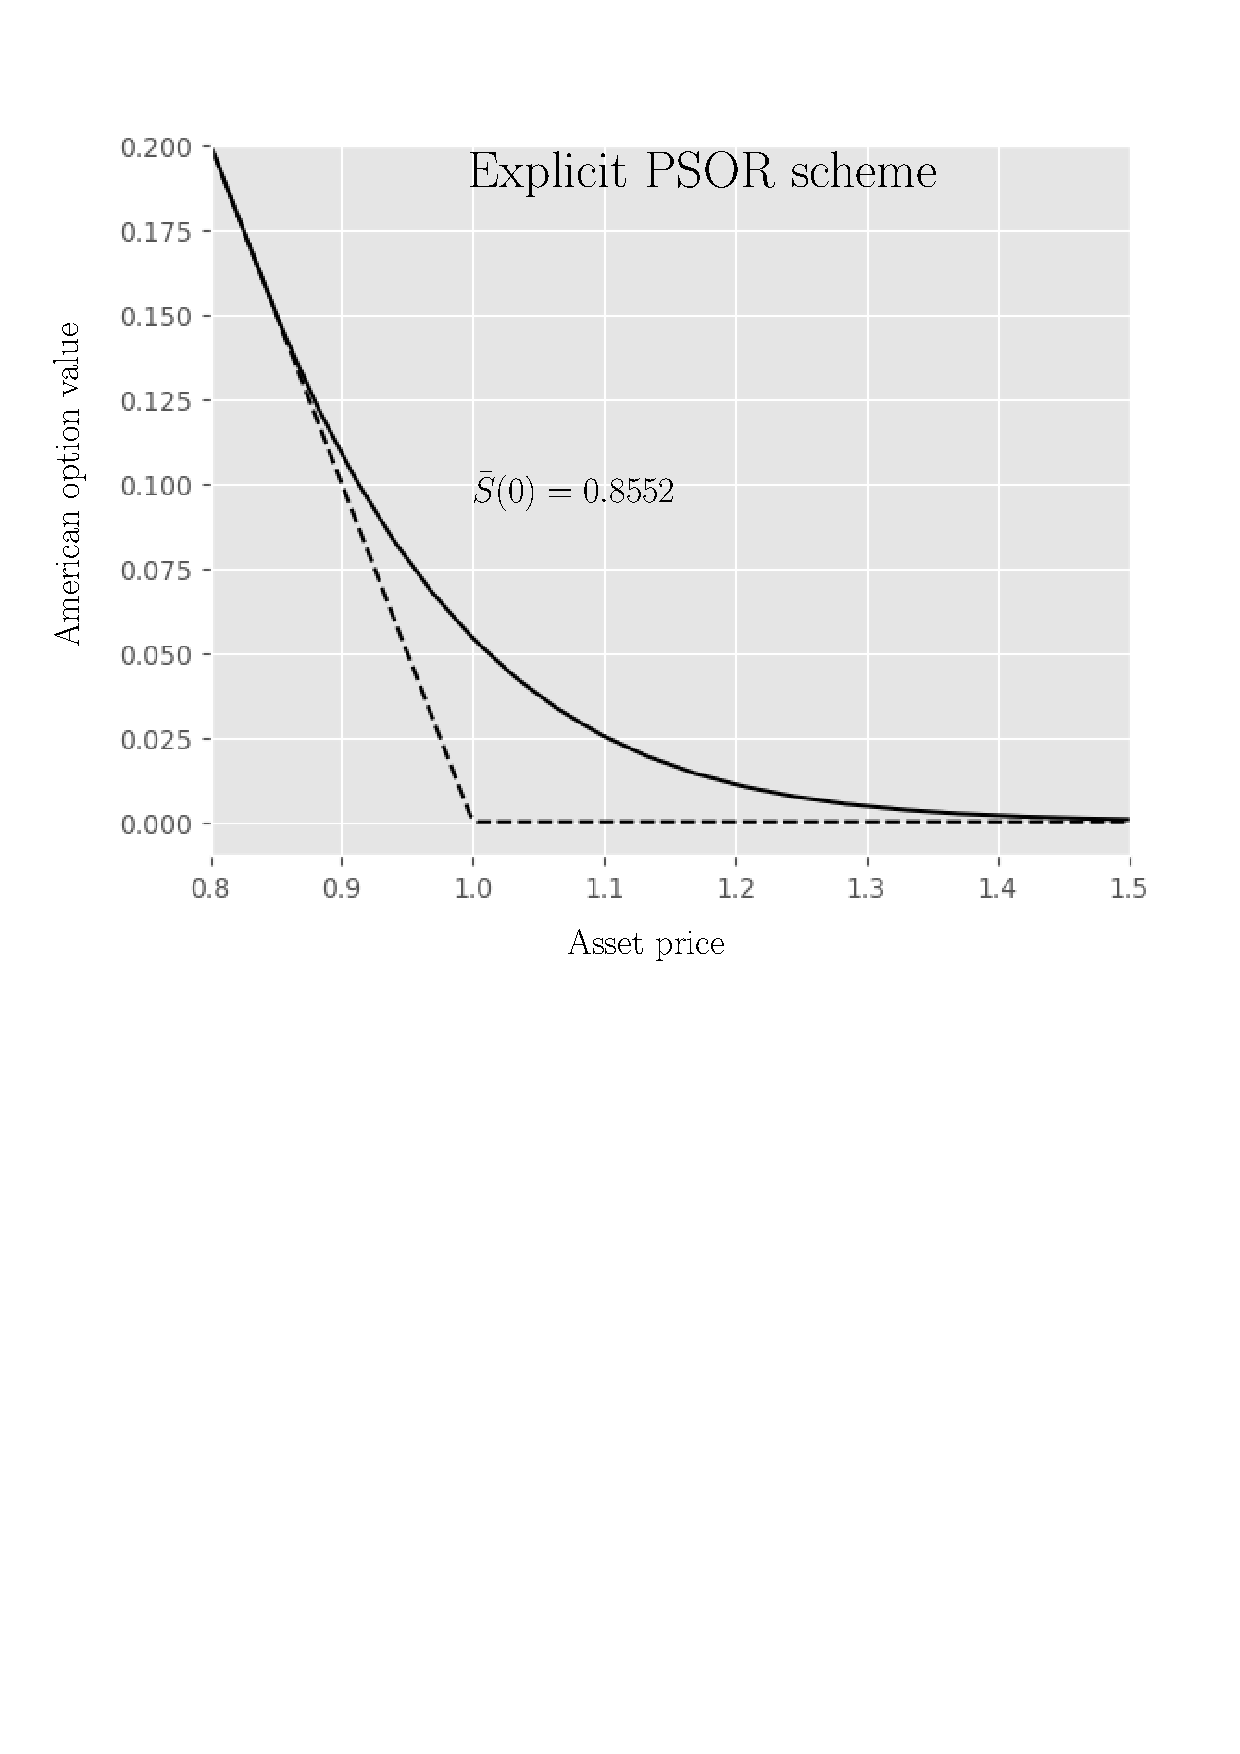
\includegraphics[width=\textwidth]{chapters/chapter5/TestCase2ExplicitLCP.pdf}
    \caption{$\Delta{x}=\expnumber{1}{-3}, \Delta{t}=0.5\times\expnumber{1}{-6}$}
    \label{fig:lcp:numericaresults:test_case_2_explicit}
  \end{subfigure}
  \begin{subfigure}{0.4\textwidth}
    \centering
    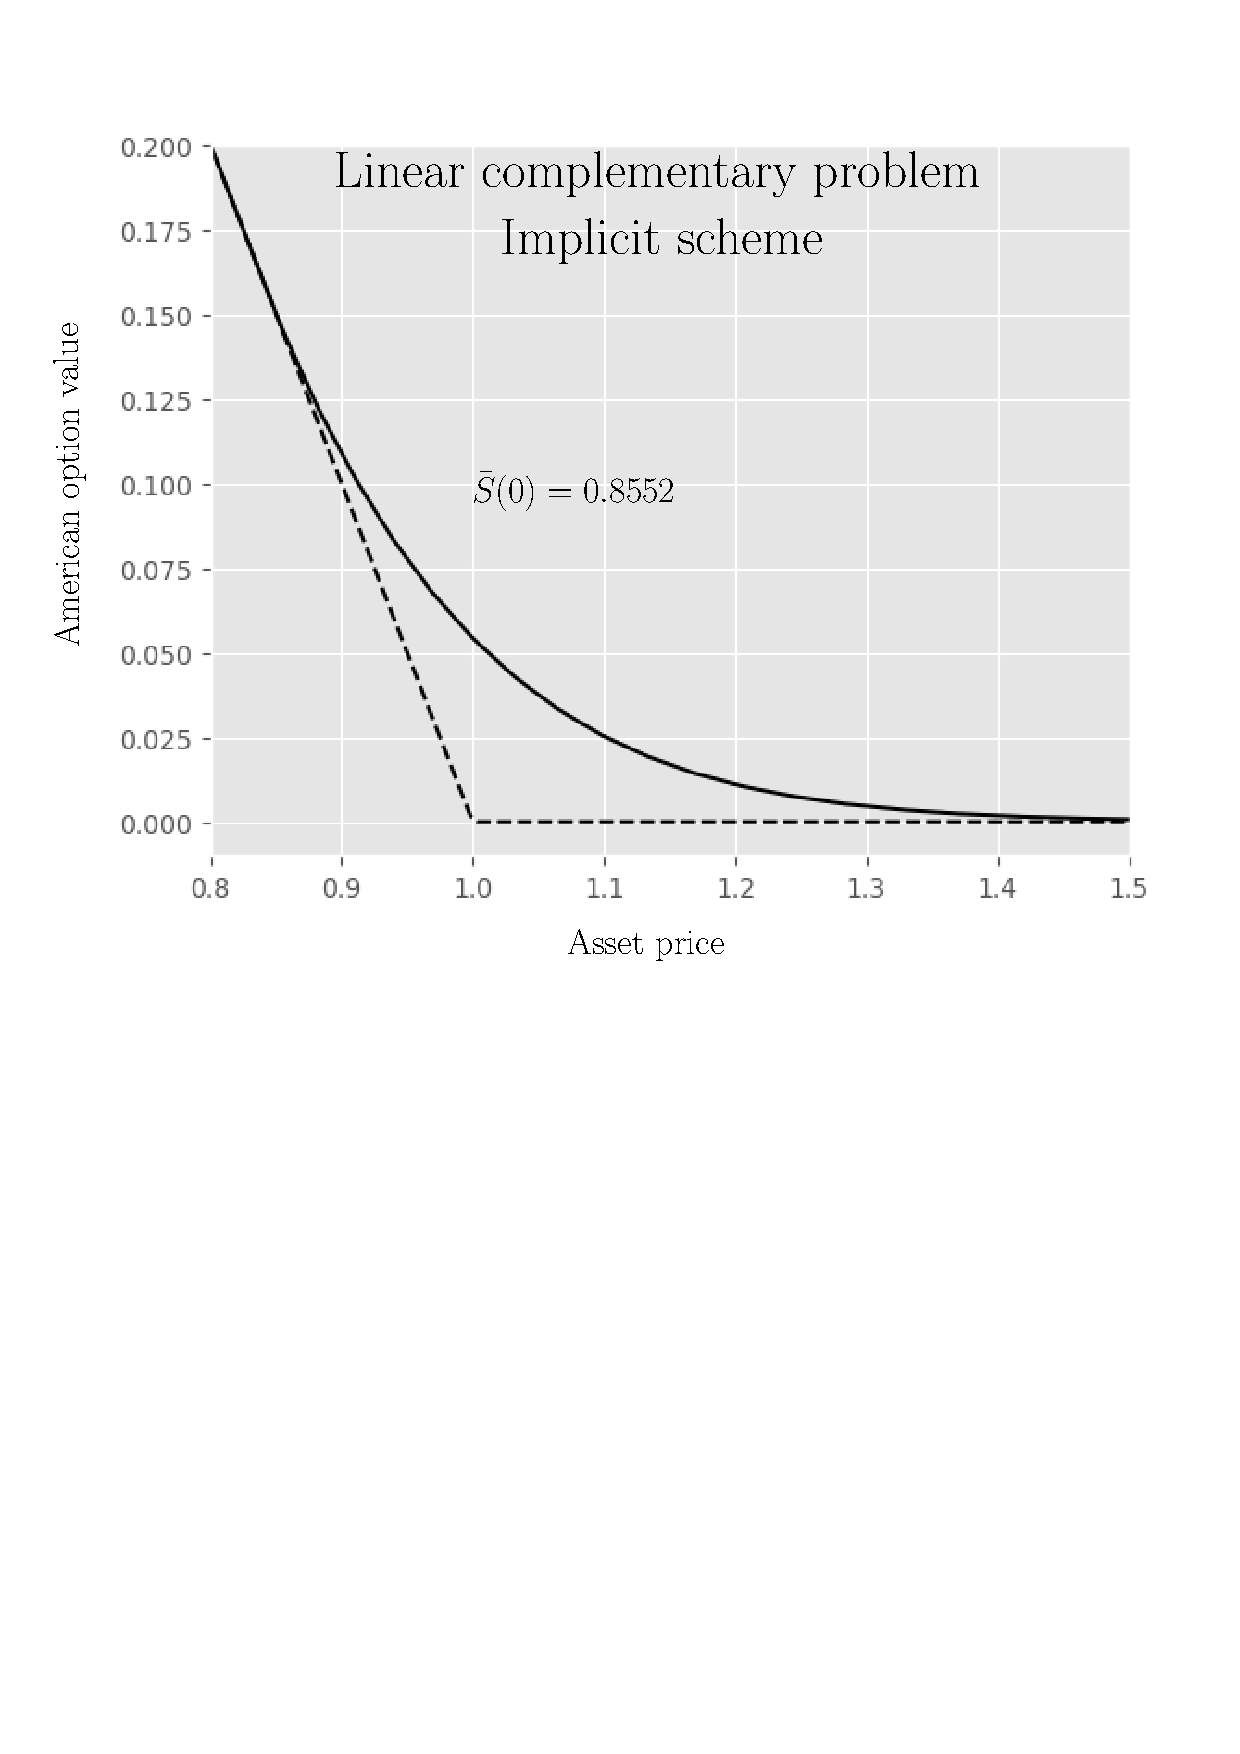
\includegraphics[width=\textwidth]{chapters/chapter5/TestCase2ImplicitLCP.pdf}
    \caption{$\Delta{x}=\expnumber{1}{-3}, \Delta{t}=0.5\times\expnumber{1}{-6}$}
    \label{fig:lcp:numericaresults:test_case_2_implicit}
  \end{subfigure}
  \hspace{0.5cm}
  \begin{subfigure}{0.4\textwidth}
    \label{fig:lcp:numericaresults:test_case_2_crank_nicholson}
    \centering
    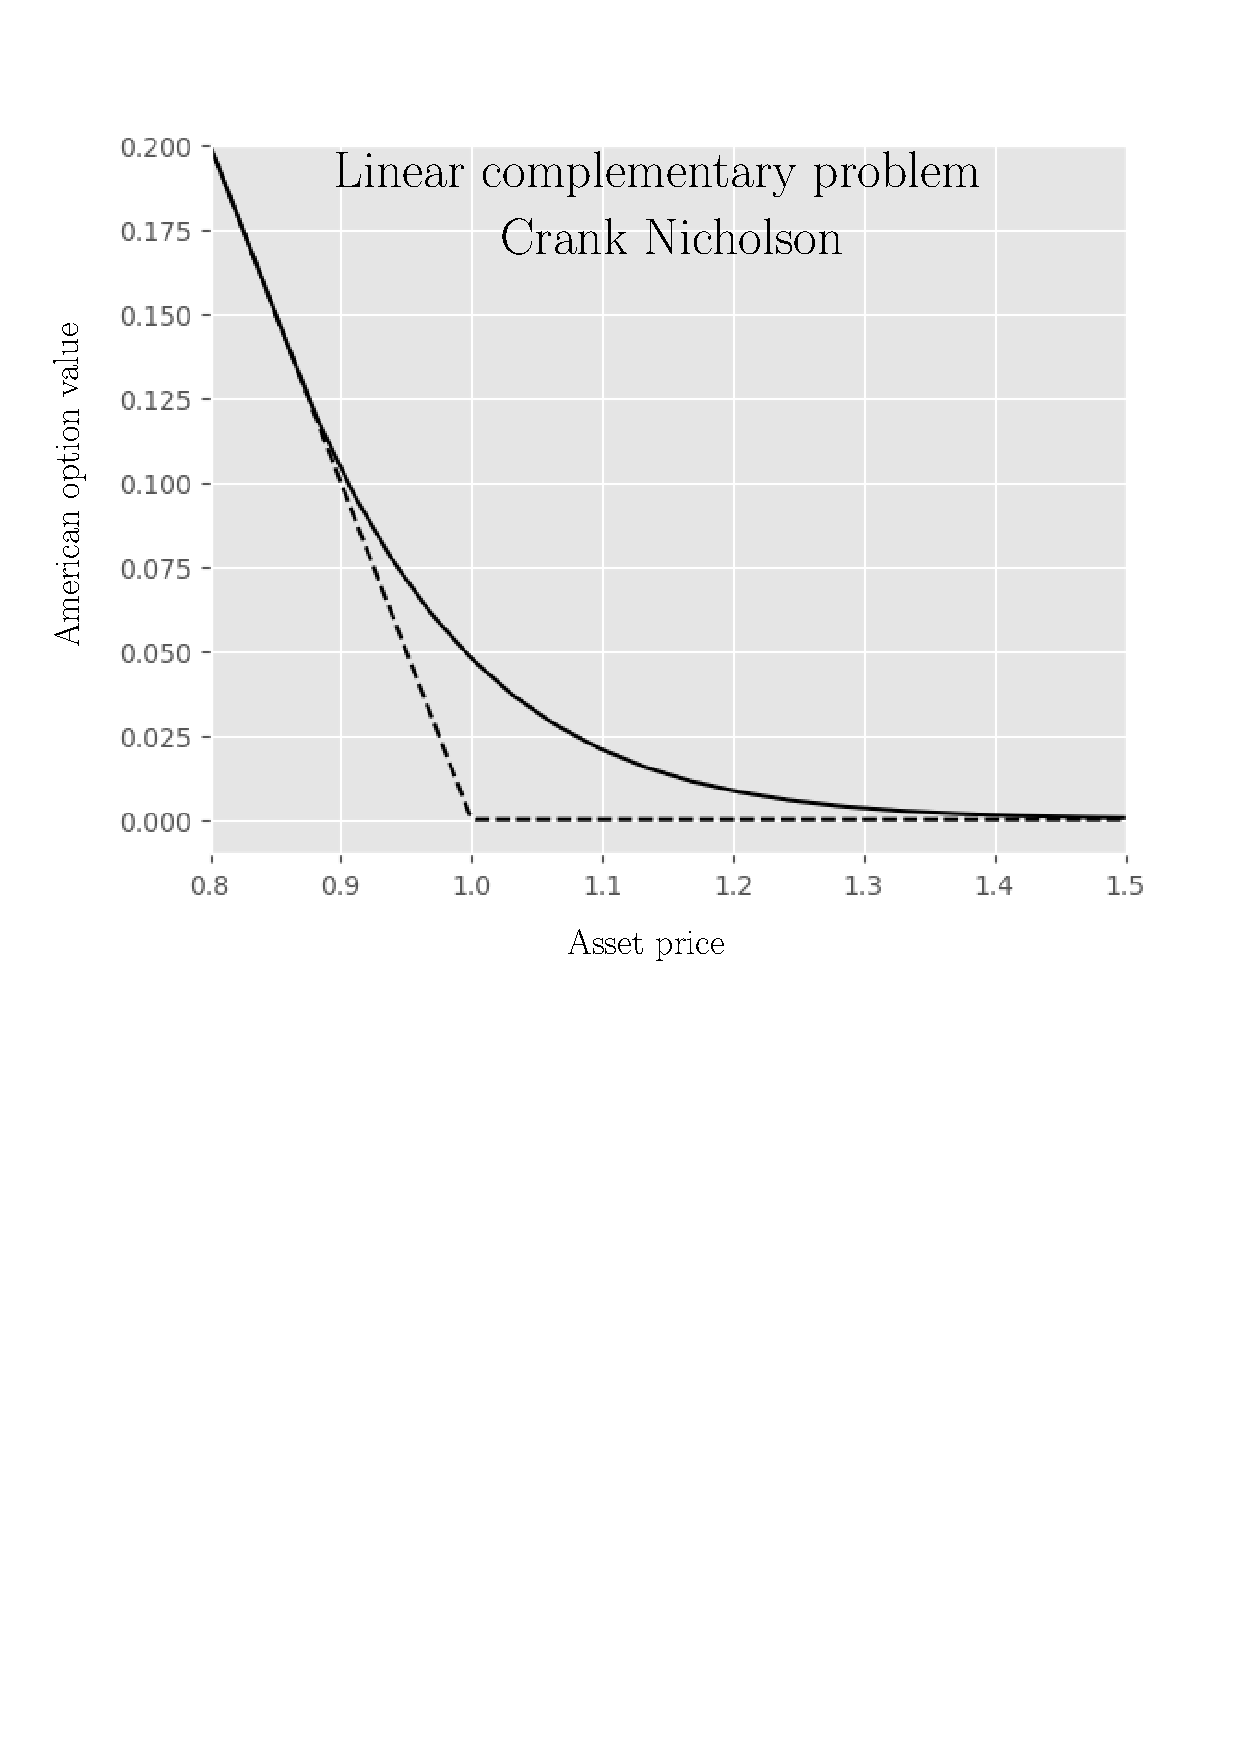
\includegraphics[width=\textwidth]{chapters/chapter5/TestCase2CrankNicholsonLCP.pdf}
    \caption{$\Delta{x}=\Delta{t}=\expnumber{1}{-3}$.}
  \end{subfigure}
  \caption{American put option value $V(S, 0)$ given parameters \eqref{eq:numericaresults:parameters_set_1}.}
  \label{fig:lcp:numericaresults:test_case_2}
\end{figure}

% Please add the following required packages to your document preamble:
% \usepackage{booktabs}
\begin{table}[H]
  \centering
  \begin{tabular}{@{}ccccc@{}}
  \toprule
  \textbf{Asset Price} & \textbf{BOPM} & \textbf{Explicit} & \textbf{Implicit} & \textbf{\begin{tabular}[c]{@{}c@{}}Crank-\\ Nicholson\end{tabular}} \\ \midrule
  0.8 & 0.200000      & 0.200000 & 0.200000 & 0.200000 \\
  1.0 & 0.048167      & 0.047919 & 0.047912 & 0.047916 \\
  1.2 & 0.008666      & 0.008646 & 0.008644 & 0.008645 \\
  1.4 & 0.001285      & 0.001296 & 0.001297 & 0.001296 \\
  1.6 & 0.000167      & 0.000170 & 0.000170 & 0.000170 \\
      & \textbf{RMSE} & 0.000111 & 0.000115 & 0.000113 \\
      & \textbf{Time} & 4609ms   & 19123ms  & 16741ms  \\ \bottomrule
  \end{tabular}
  \caption{
  \label{tab:lcp:test_case_2}  $V(S, 0)$ put approximation given parameters \eqref{eq:numericaresults:parameters_set_1}.}
\end{table}

\begin{figure}[tbp]
  \centering
  \begin{subfigure}{0.4\textwidth}
    \centering
    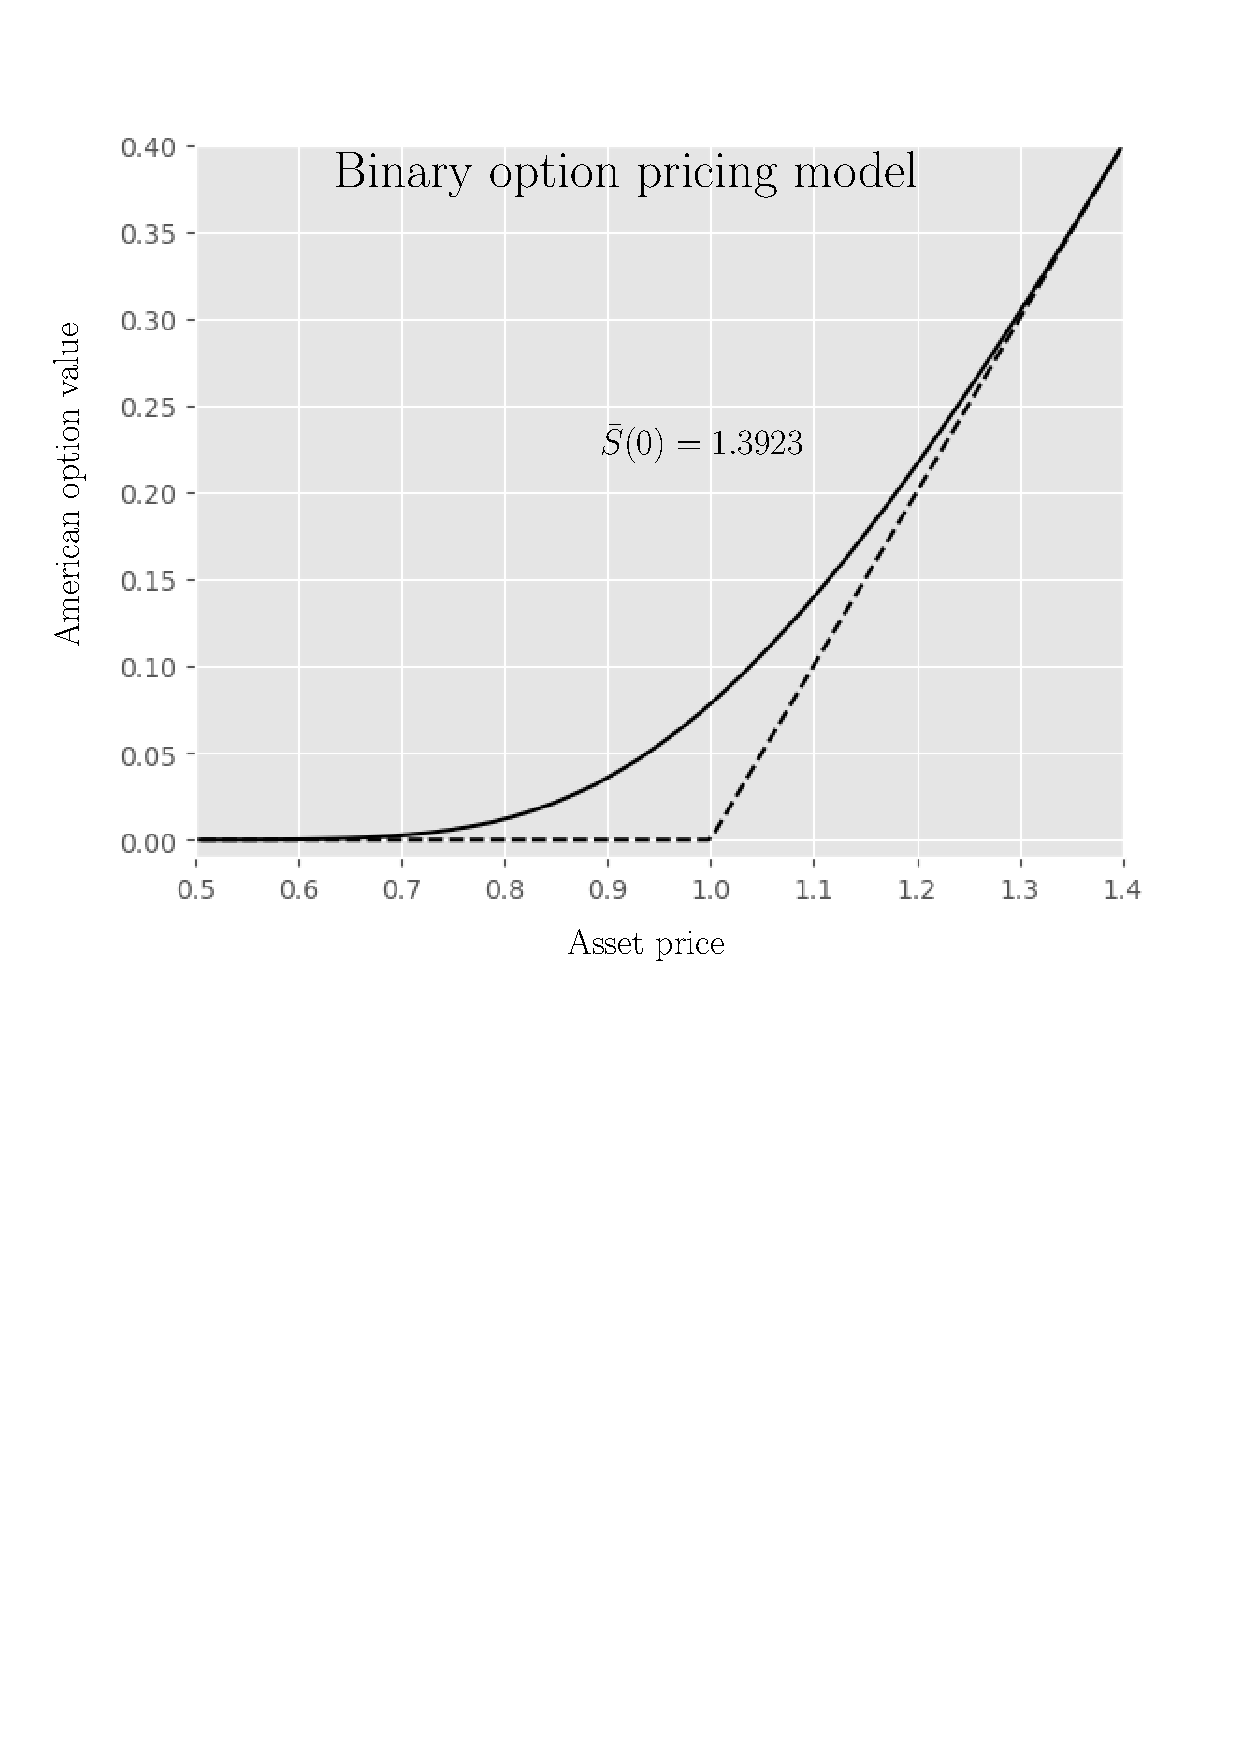
\includegraphics[width=\textwidth]{chapters/chapter5/TestCase3LcpBOPM.pdf}
    \caption{$\text{Nodes} = 2^{500}$.}
    \label{fig:lcp:numericaresults:test_case_3_bopm}
  \end{subfigure}
  \hspace{0.5cm}
  \begin{subfigure}{0.4\textwidth}
    \centering
    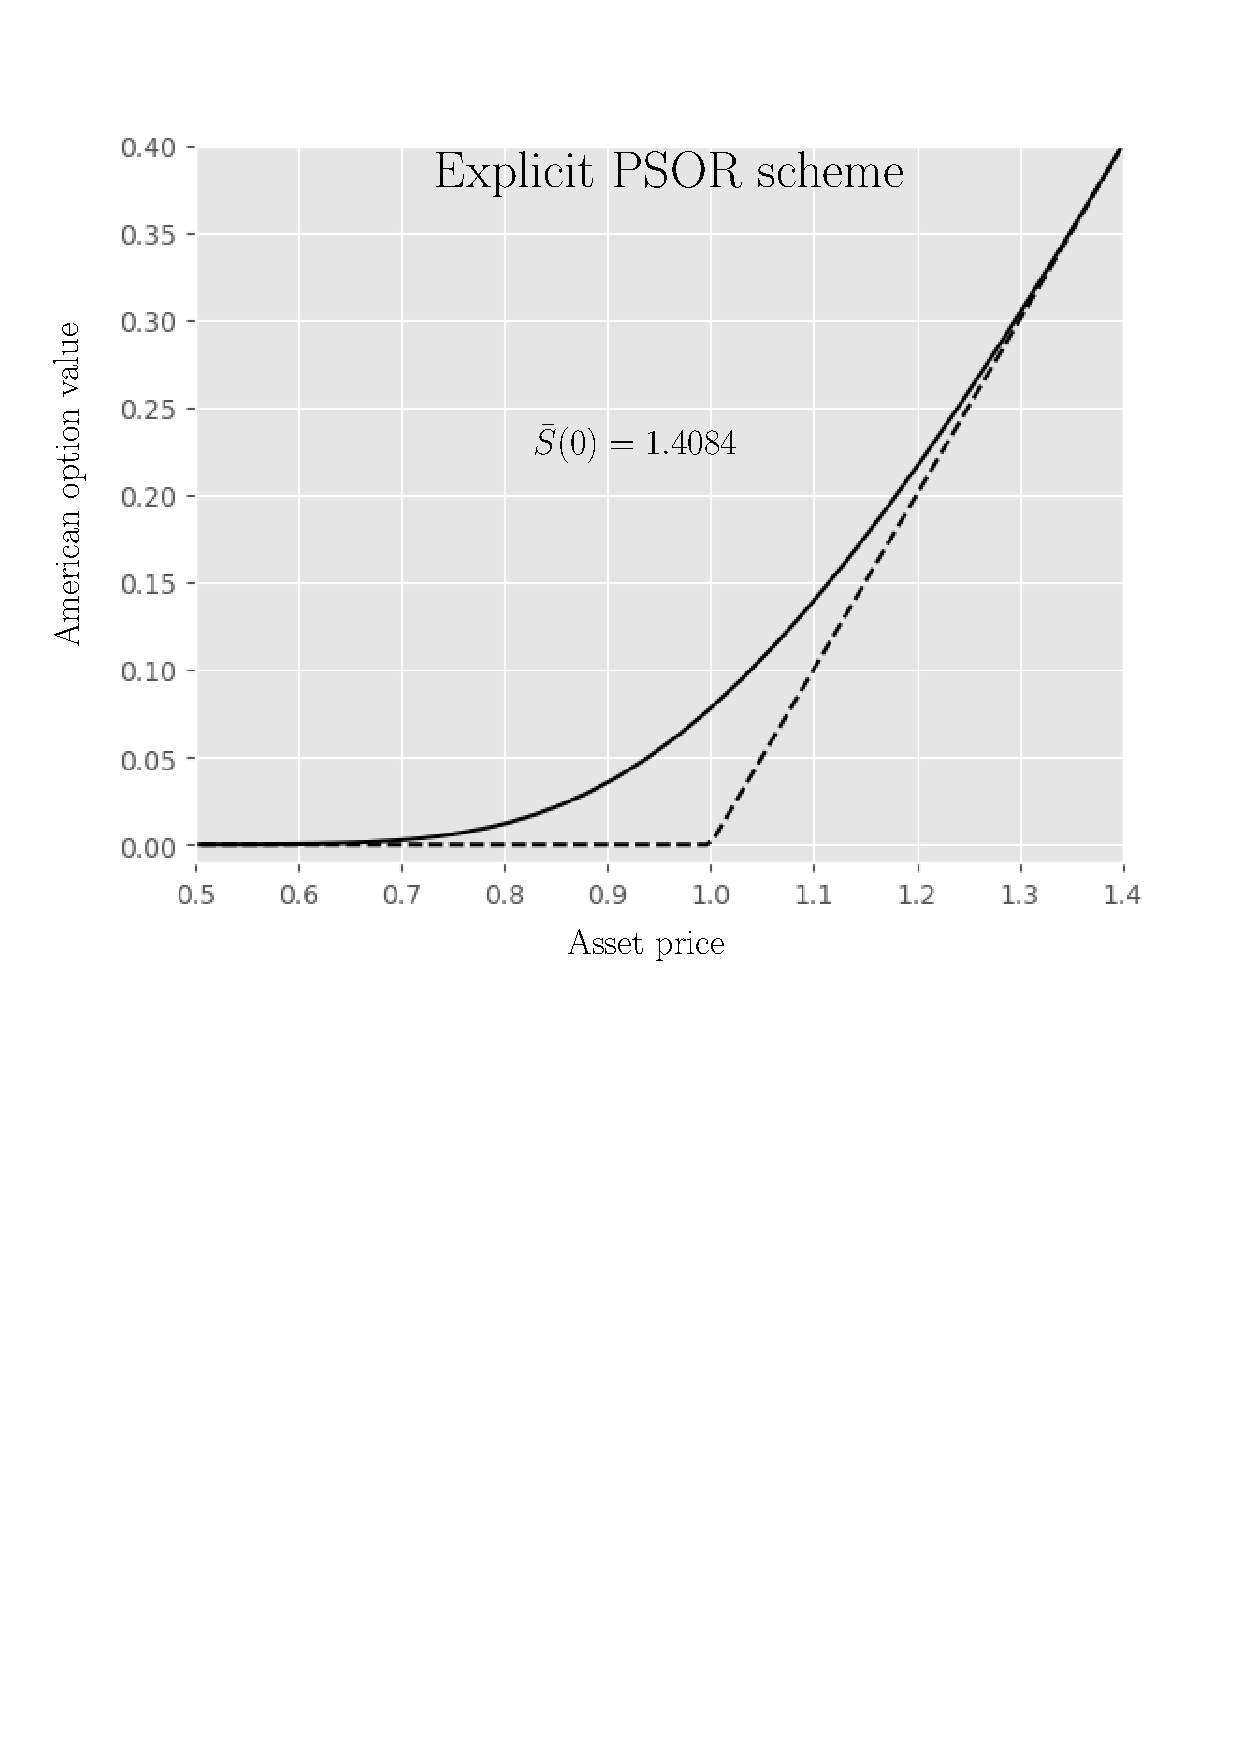
\includegraphics[width=\textwidth]{chapters/chapter5/TestCase3ExplicitLCP.pdf}
    \caption{$\Delta{x}=\expnumber{1}{-3}, \Delta{t}=0.5\times\expnumber{1}{-6}$}
    \label{fig:lcp:numericaresults:test_case_3_explicit}
  \end{subfigure}
  \begin{subfigure}{0.4\textwidth}
    \centering
    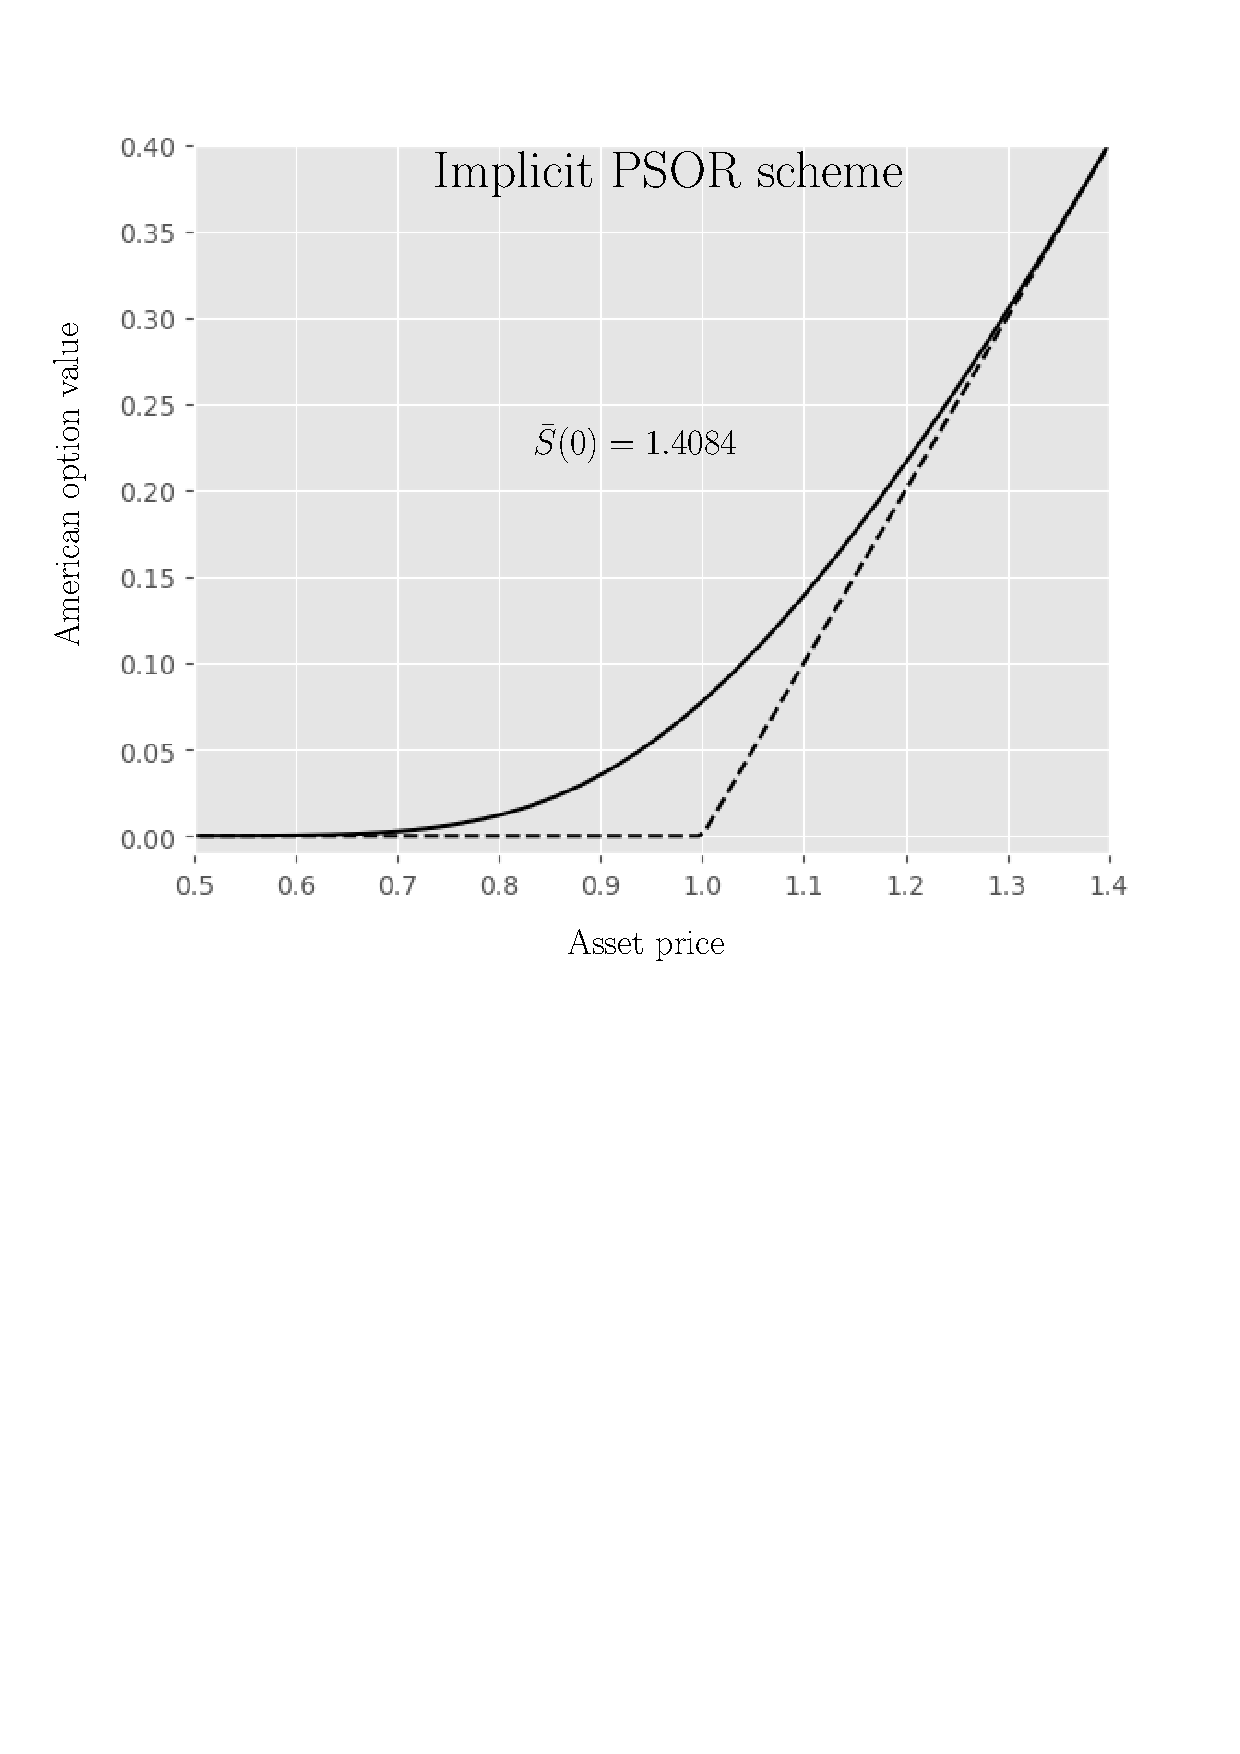
\includegraphics[width=\textwidth]{chapters/chapter5/TestCase3ImplicitLCP.pdf}
    \caption{$\Delta{x}=\expnumber{1}{-3}, \Delta{t}=0.5\times\expnumber{1}{-6}$}
    \label{fig:lcp:numericaresults:test_case_3_implicit}
  \end{subfigure}
  \hspace{0.5cm}
  \begin{subfigure}{0.4\textwidth}
    \label{fig:lcp:numericaresults:test_case_3_crank_nicholson}
    \centering
    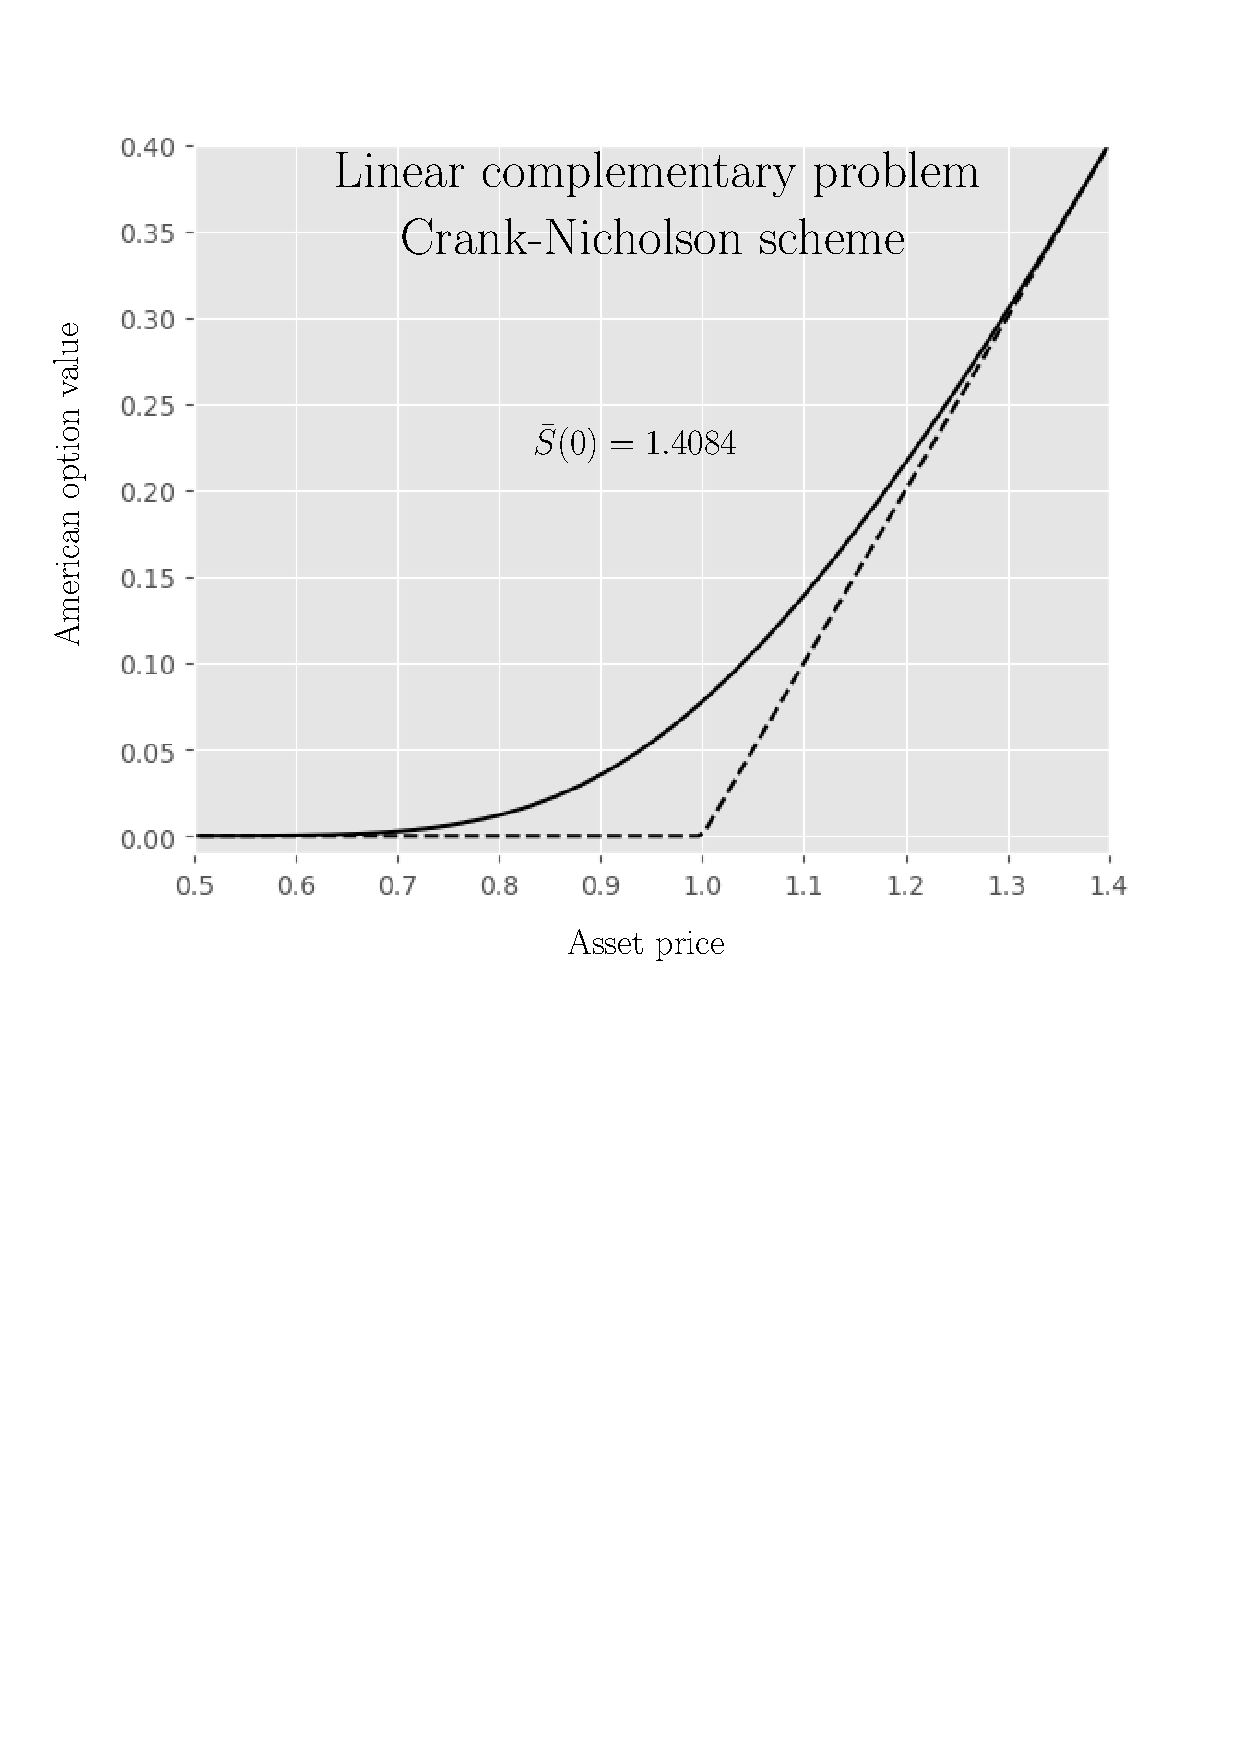
\includegraphics[width=\textwidth]{chapters/chapter5/TestCase3CrankNicholsonLCP.pdf}
    \caption{$\Delta{x}=\Delta{t}=\expnumber{1}{-3}$.}
  \end{subfigure}
  \caption{American call option value $V(S, 0)$ given parameters \eqref{eq:numericaresults:parameters_set_3}.}
  \label{fig:lcp:numericaresults:test_case_3}
\end{figure}

% Please add the following required packages to your document preamble:
% \usepackage{booktabs}
\begin{table}[H]
  \centering
  \begin{tabular}{@{}ccccc@{}}
  \toprule
  \textbf{Asset Price} & \textbf{BOPM} & \textbf{Explicit} & \textbf{Implicit} & \textbf{\begin{tabular}[c]{@{}c@{}}Crank-\\ Nicholson\end{tabular}} \\ \midrule
  0.8 & 0.011962      & 0.011949 & 0.0120106 & 0.011962 \\
  1.0 & 0.078062      & 0.077858 & 0.0775714 & 0.078062 \\
  1.2 & 0.215901      & 0.021586 & 0.2157617 & 0.215901 \\
  1.4 & 0.400000      & 0.400090 & 0.4000923 & 0.400000 \\
  1.6 & 0.600000      & 0.600000 & 0.6000000 & 0.600000 \\
      & \textbf{RMSE} & 0.000072 & 0.000166  & 0.000074 \\
      & \textbf{Time} & 4640ms   & 1821ms    & 1310ms   \\ \bottomrule
  \end{tabular}
  \caption{
  \label{tab:lcp:test_case_3} $V(S, 0)$ put approximation given parameters \eqref{eq:numericaresults:parameters_set_3}.}
\end{table}

\begin{figure}[H]
  \centering
  \begin{subfigure}{0.4\textwidth}
    \centering
    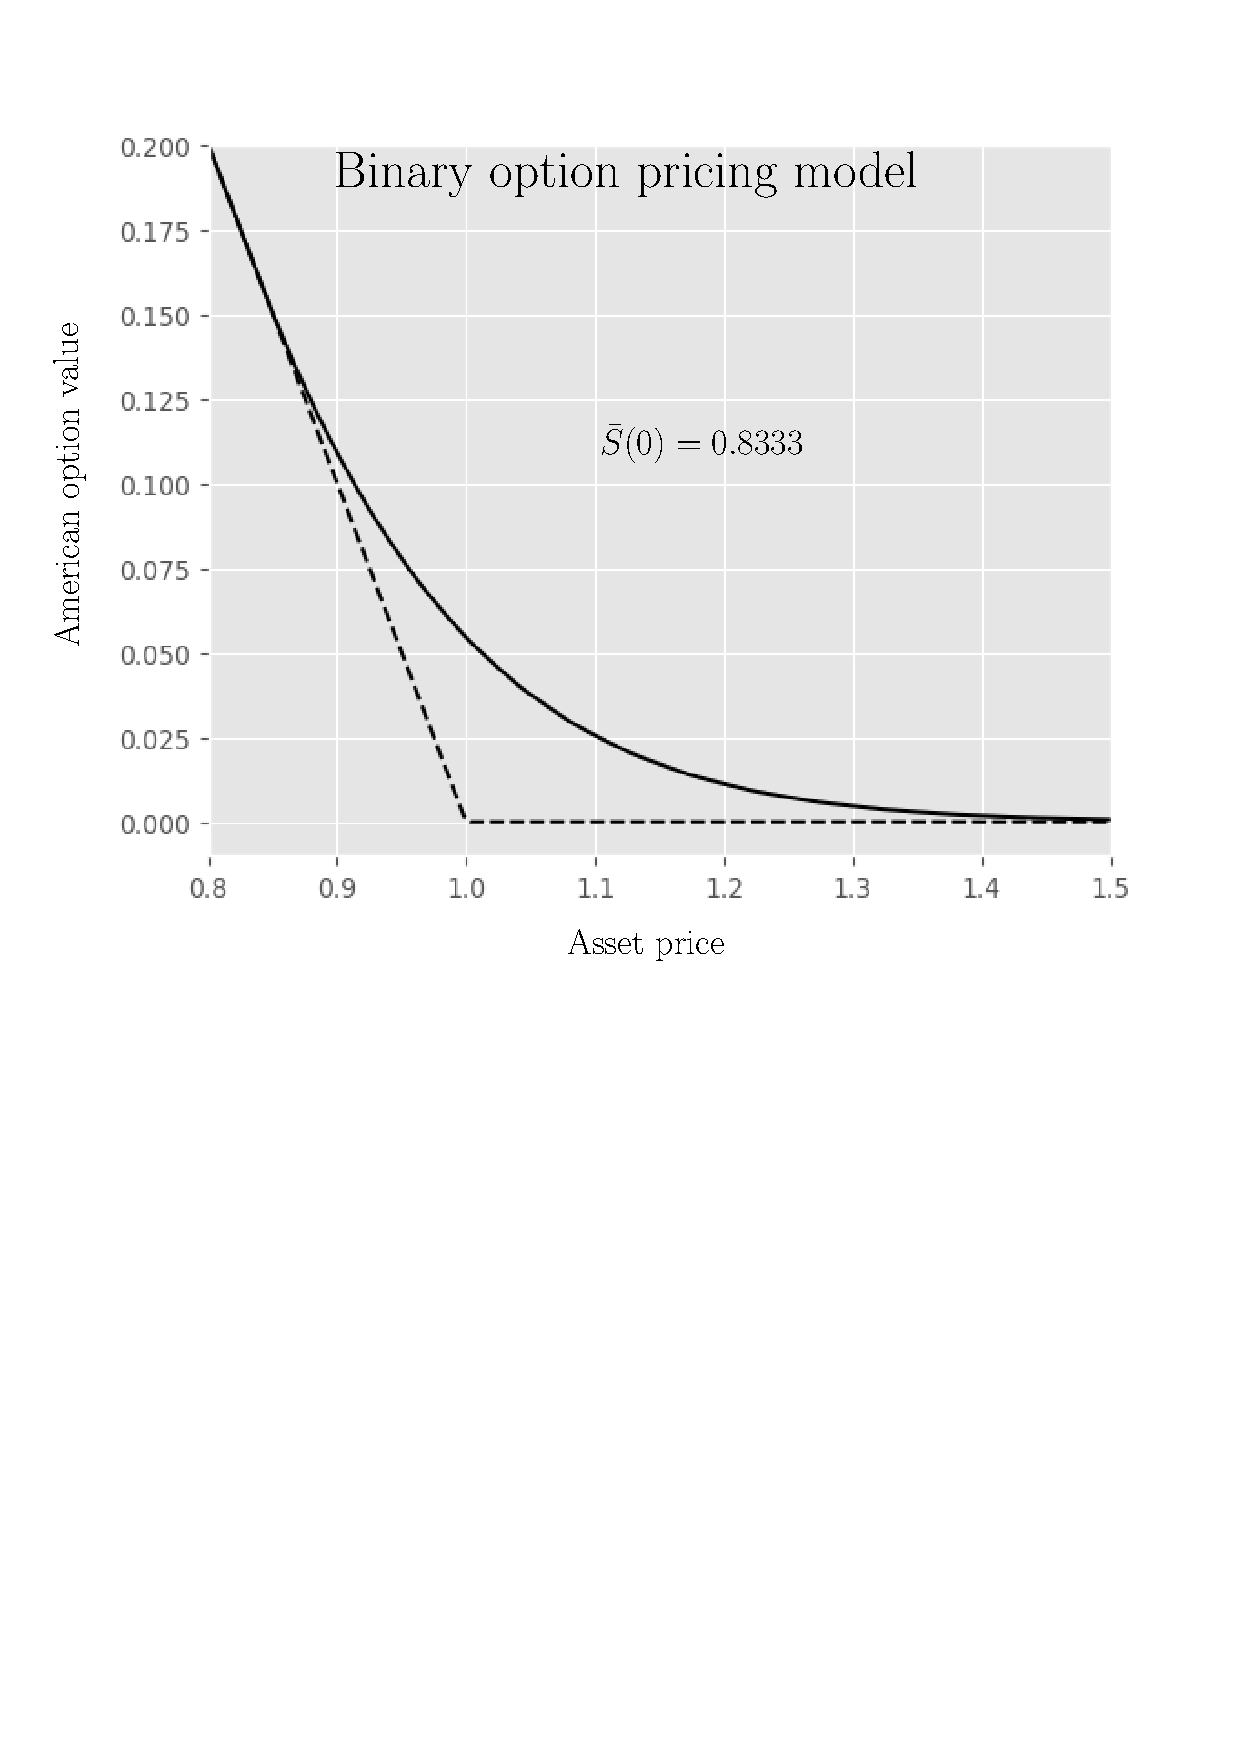
\includegraphics[width=\textwidth]{chapters/chapter5/TestCase4LcpBOPM.pdf}
    \caption{$\text{Nodes} = 2^{500}$.}
    \label{fig:lcp:numericaresults:test_case_4_bopm}
  \end{subfigure}
  \hspace{0.5cm}
  \begin{subfigure}{0.4\textwidth}
    \centering
    \includegraphics[width=\textwidth]{chapters/chapter5/TestCase4ExplicitLCP.pdf}
    \caption{$\Delta{x}=\expnumber{1}{-3}, \Delta{t}=0.5\times\expnumber{1}{-6}$}
    \label{fig:lcp:numericaresults:test_case_4_explicit}
  \end{subfigure}
  \begin{subfigure}{0.4\textwidth}
    \centering
    \includegraphics[width=\textwidth]{chapters/chapter5/TestCase4ImplicitLCP.pdf}
    \caption{$\Delta{x}=\expnumber{1}{-3}, \Delta{t}=0.5\times\expnumber{1}{-6}$}
    \label{fig:lcp:numericaresults:test_case_4_implicit}
  \end{subfigure}
  \hspace{0.5cm}
  \begin{subfigure}{0.4\textwidth}
    \label{fig:lcp:numericaresults:test_case_4_crank_nicholson}
    \centering
    \includegraphics[width=\textwidth]{chapters/chapter5/TestCase4CrankNicholsonLCP.pdf}
    \caption{$\Delta{x}=\Delta{t}=\expnumber{1}{-3}$.}
  \end{subfigure}
  \caption{American put option value $V(S, 0)$ given parameters \eqref{eq:numericaresults:parameters_set_4}.}
  \label{fig:lcp:numericaresults:test_case_4}
\end{figure}

% Please add the following required packages to your document preamble:
% \usepackage{booktabs}
\begin{table}[H]
  \centering
  \begin{tabular}{@{}ccccc@{}}
  \toprule
  \textbf{Asset Price} & \textbf{BOPM} & \textbf{Explicit} & \textbf{Implicit} & \textbf{\begin{tabular}[c]{@{}c@{}}Crank-\\ Nicholson\end{tabular}} \\ \midrule
  0.8 & 0.200000      & 0.200000 & 0.200000 & 0.200000 \\
  1.0 & 0.054464      & 0.054246 & 0.053968 & 0.054239 \\
  1.2 & 0.011255      & 0.011134 & 0.011063 & 0.011129 \\
  1.4 & 0.001855      & 0.001860 & 0.001908 & 0.001858 \\
  1.6 & 0.000262      & 0.000268 & 0.000300 & 0.000268 \\
      & \textbf{RMSE} & 0.000083 & 0.000179 & 0.000086 \\
      & \textbf{Time} & 4585ms   & 1310ms   & 885ms    \\ \bottomrule
  \end{tabular}
  \caption{
  \label{tab:lcp:test_case_4} $V(S, 0)$ put approximation given parameters \eqref{eq:numericaresults:parameters_set_4}.}
\end{table}

\subsubsection{Convergence Analysis}

\begin{figure}[tbp]
  \centering
  \begin{subfigure}{0.4\textwidth}
    \centering
    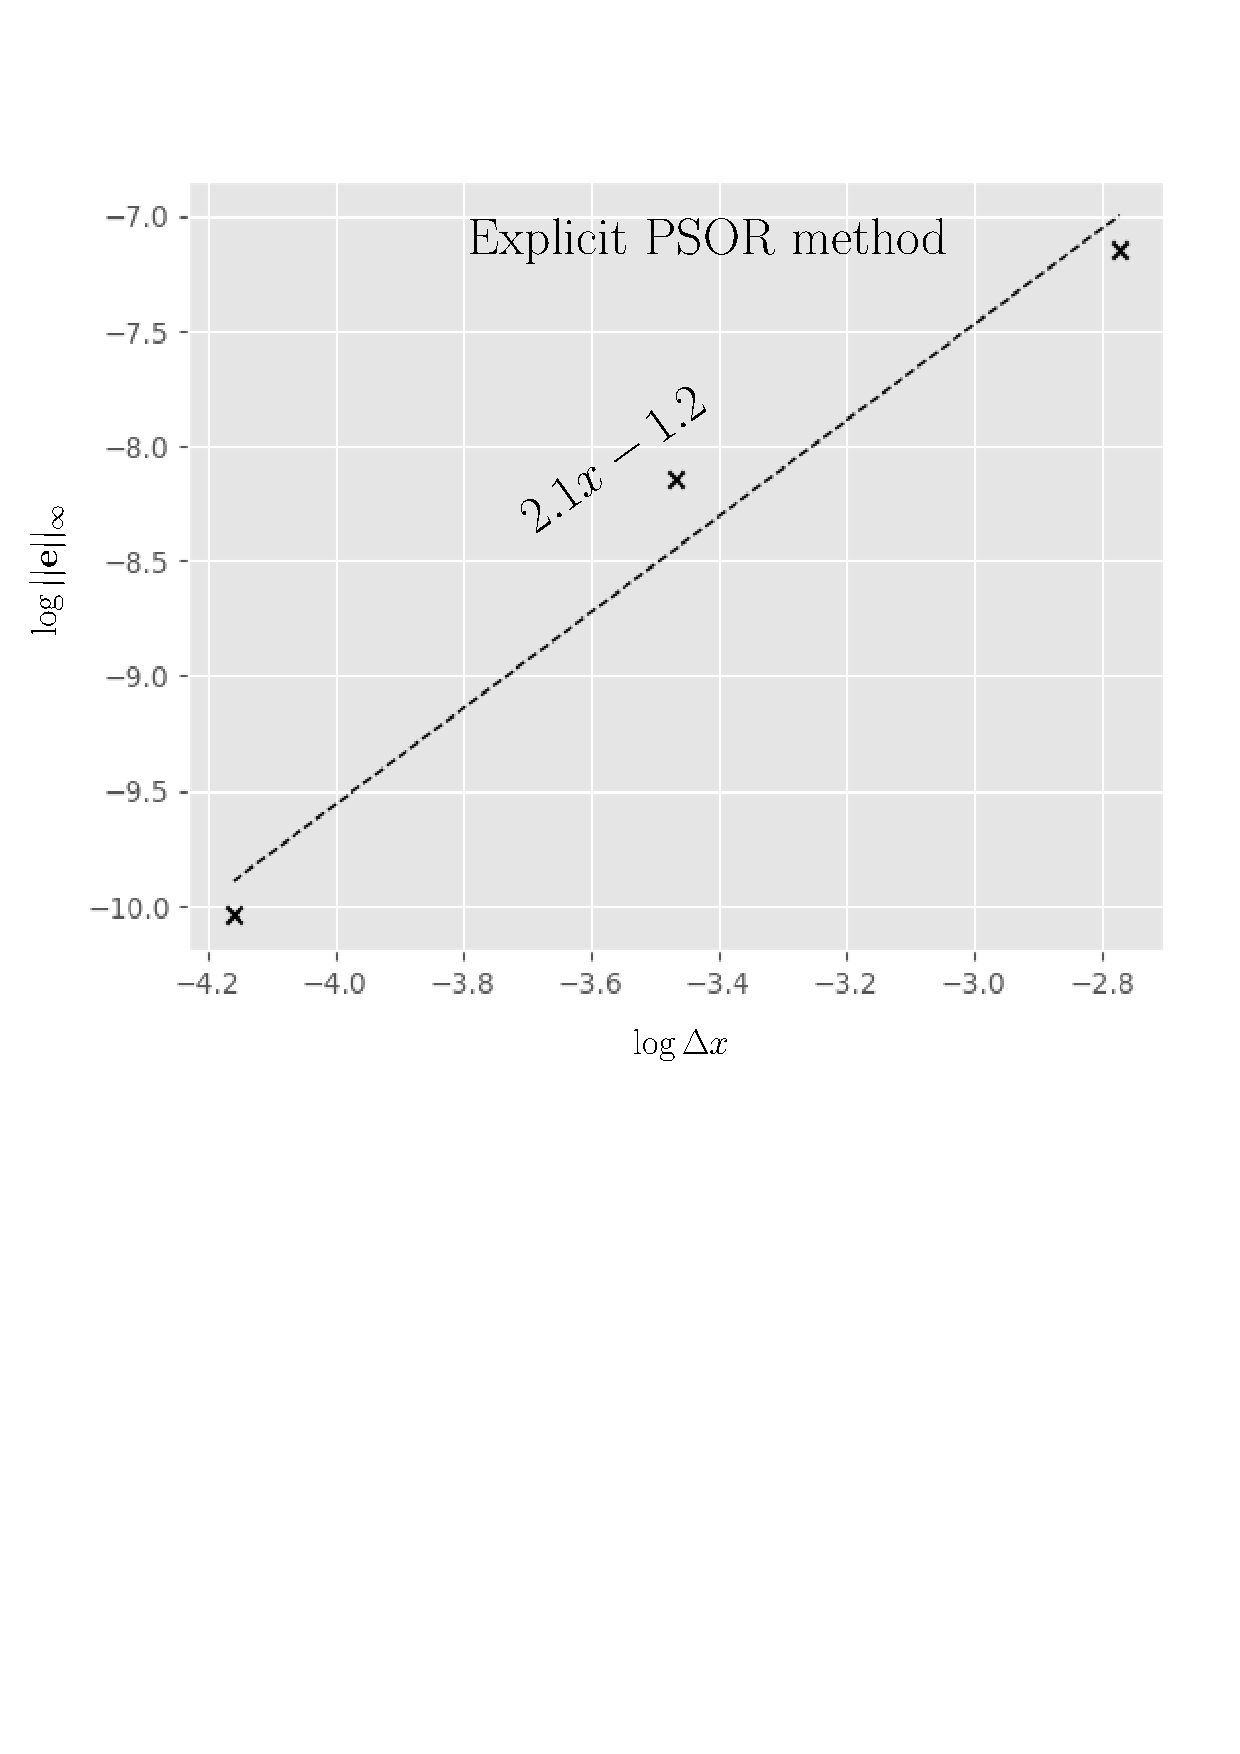
\includegraphics[width=\textwidth]{chapters/chapter5/ConvergenceSpaceExplicitLCP.pdf}
    \caption{$\Delta{x}=2^{-7},\dots,2^{-10}$}
    \caption*{$\Delta{t}=2^{-21}$}
    \label{fig:lcp:numericalresults:convergence_space_explicit}
  \end{subfigure}
  \hspace{0.5cm}
  \begin{subfigure}{0.4\textwidth}
    \centering
    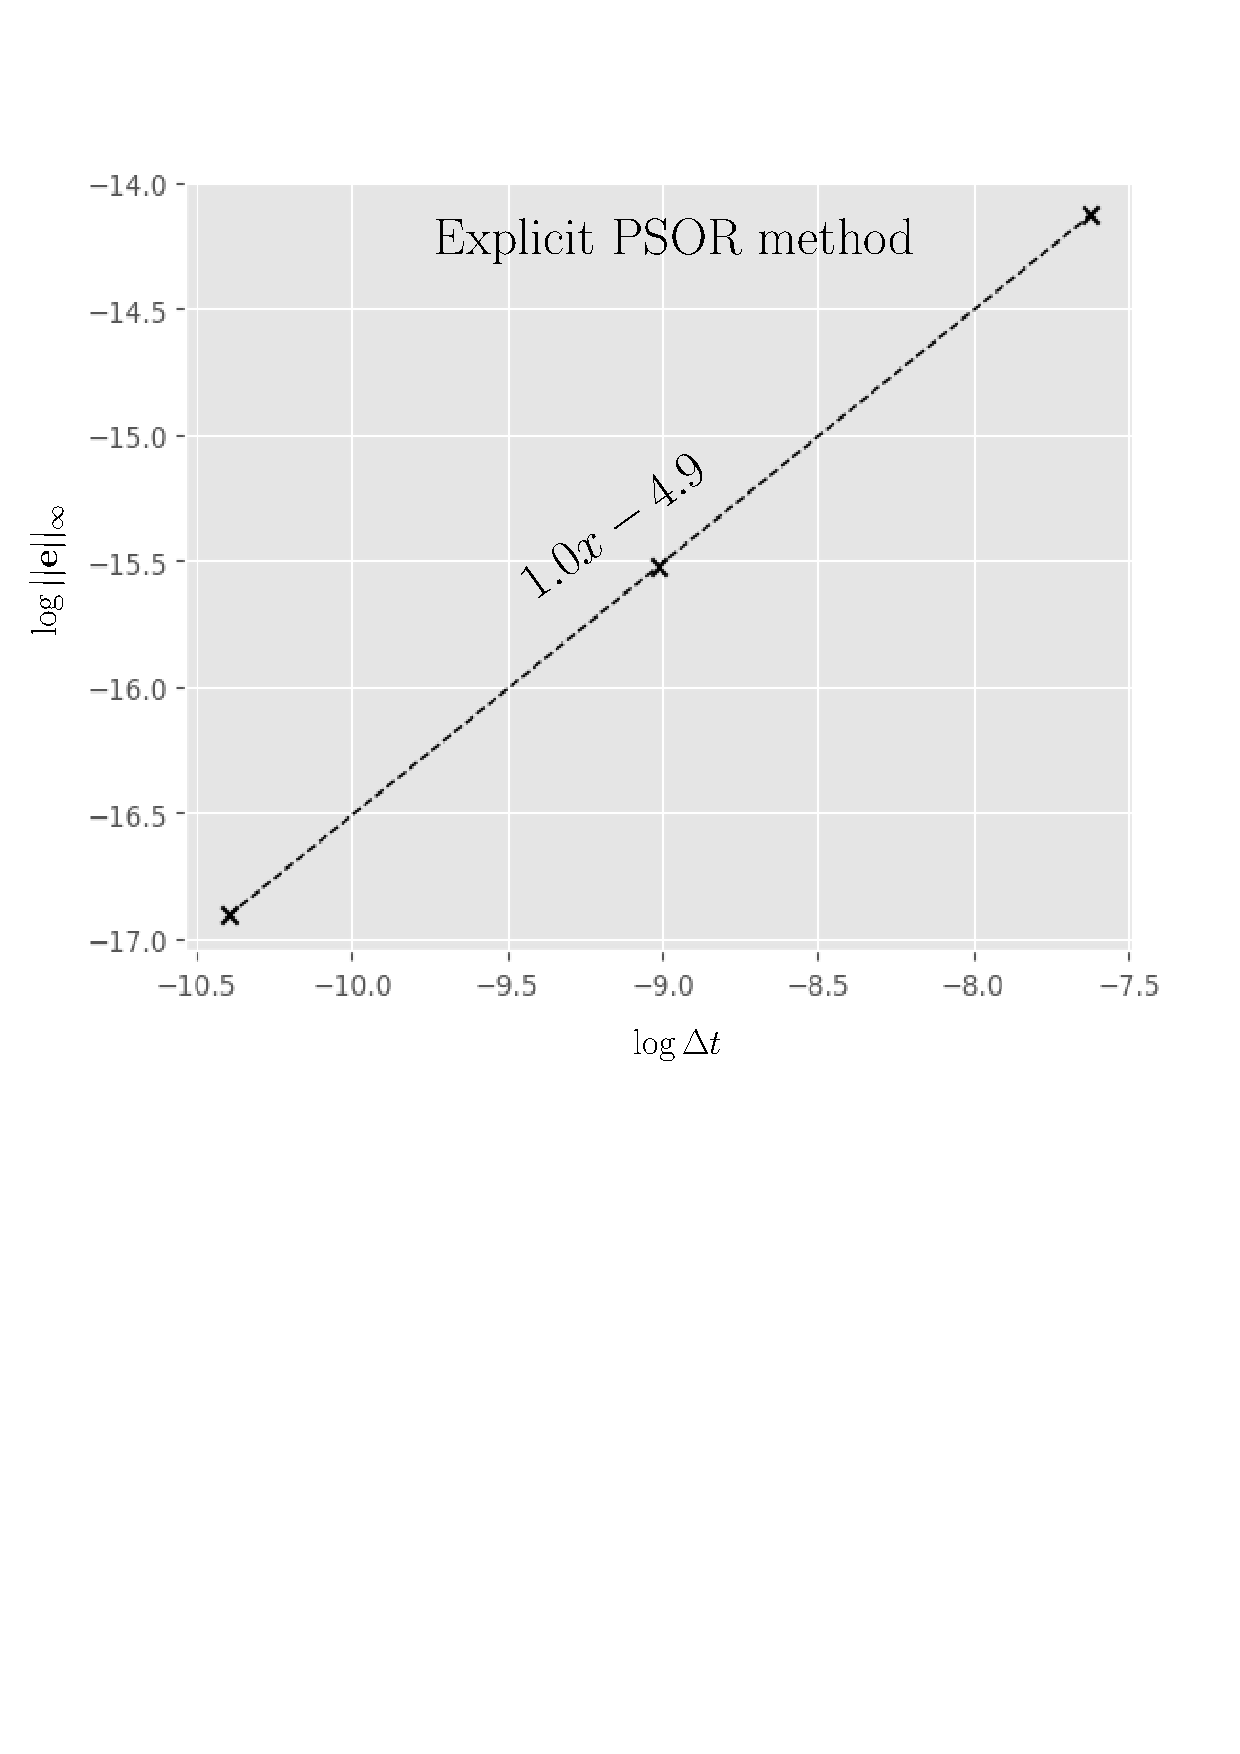
\includegraphics[width=\textwidth]{chapters/chapter5/ConvergenceTimeExplicitLCP.pdf}
    \caption{$\Delta{t}=2^{-15},2^{-17},\dots,2^{-21}$}
    \caption*{$\Delta{x}=2^{-7}$}
    \label{fig:lcp:numericalresults:convergence_time_explicit}
  \end{subfigure}
  \caption{Convergence analysis for the explicit method for the Company transformation.}
  \label{fig:lcp:numericalresults:company_convergence_analysis}
\end{figure}

\begin{figure}[tbp]
  \centering
  \begin{subfigure}{0.4\textwidth}
    \centering
    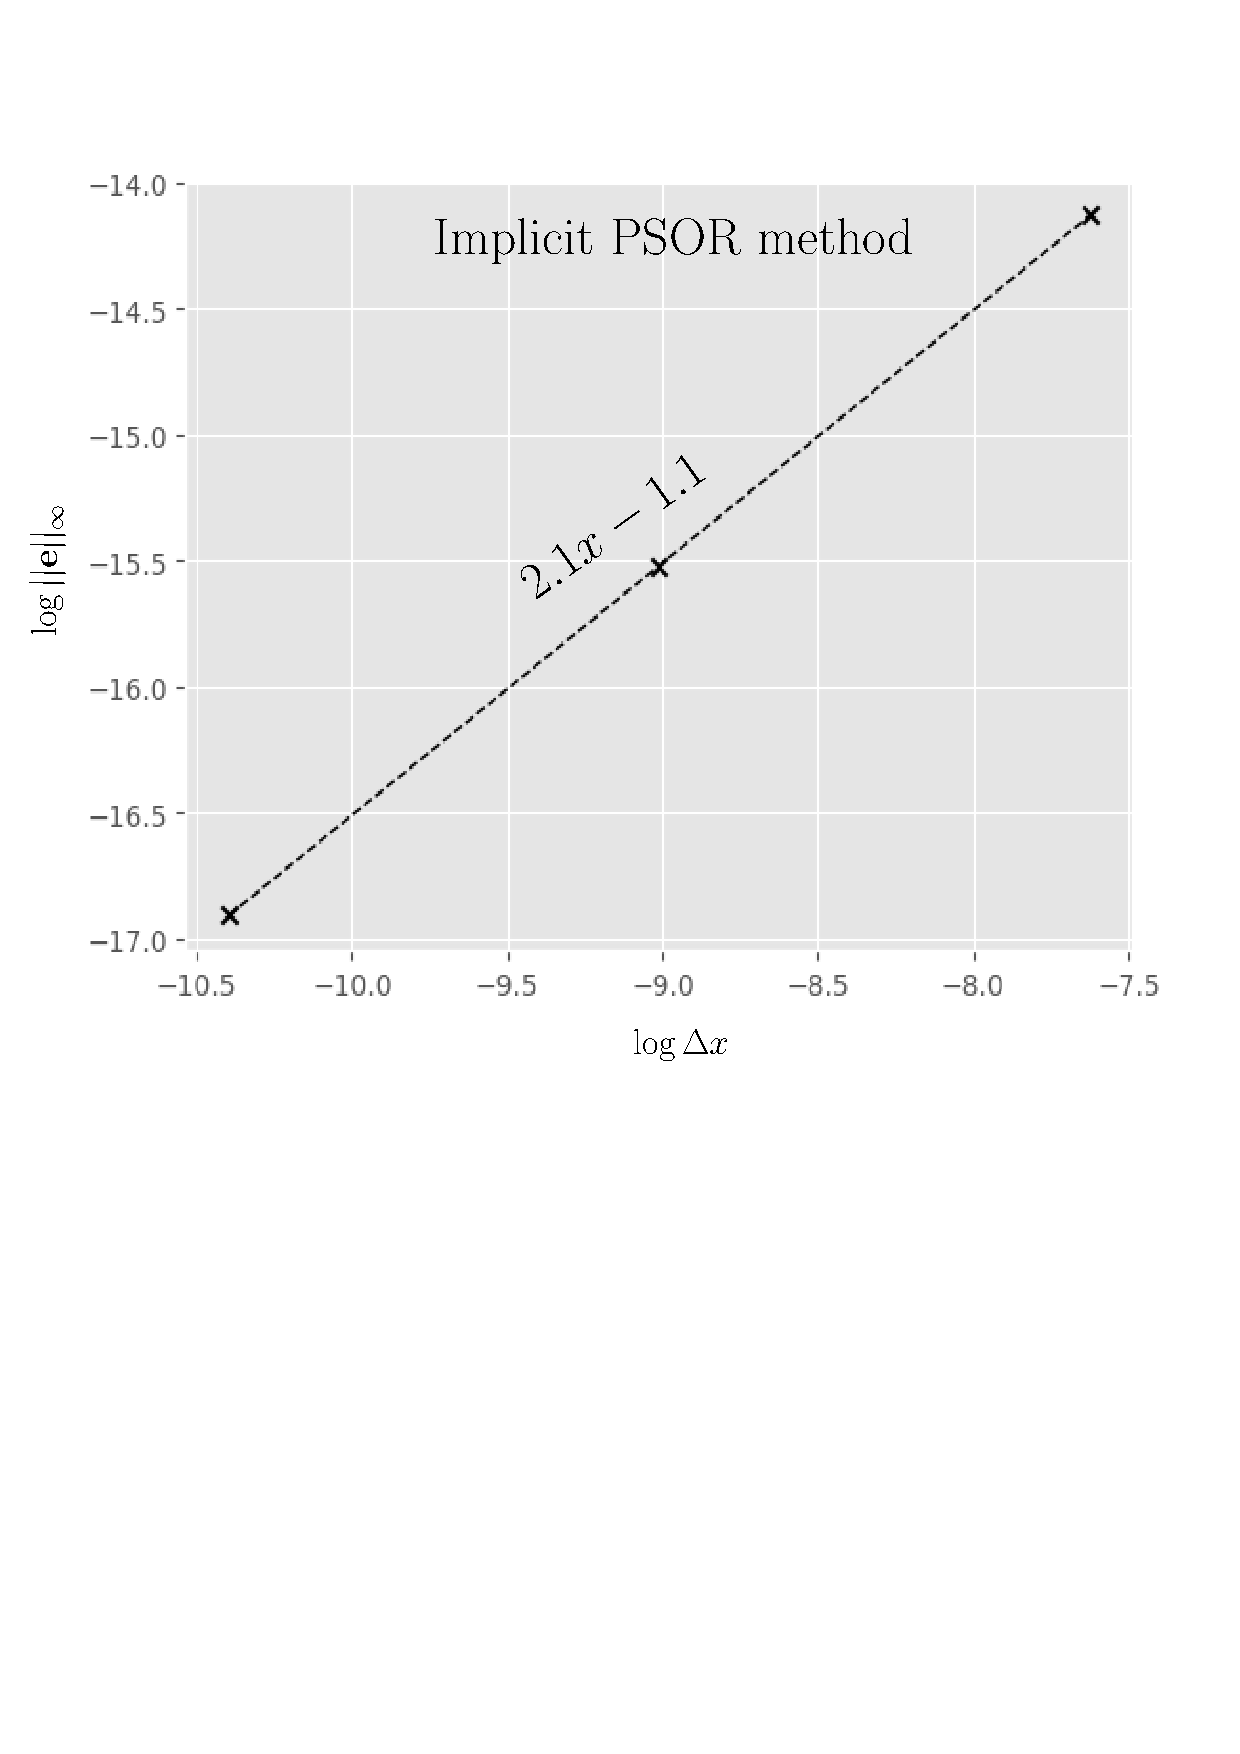
\includegraphics[width=\textwidth]{chapters/chapter5/ConvergenceSpaceImplicitLCP.pdf}
    \caption{$\Delta{x}=2^{-7},\dots,2^{-10}$}
    \caption*{$\Delta{t}=2^{-21}$}
    \label{fig:lcp:numericalresults:convergence_space_implicit}
  \end{subfigure}
  \hspace{0.5cm}
  \begin{subfigure}{0.4\textwidth}
    \centering
    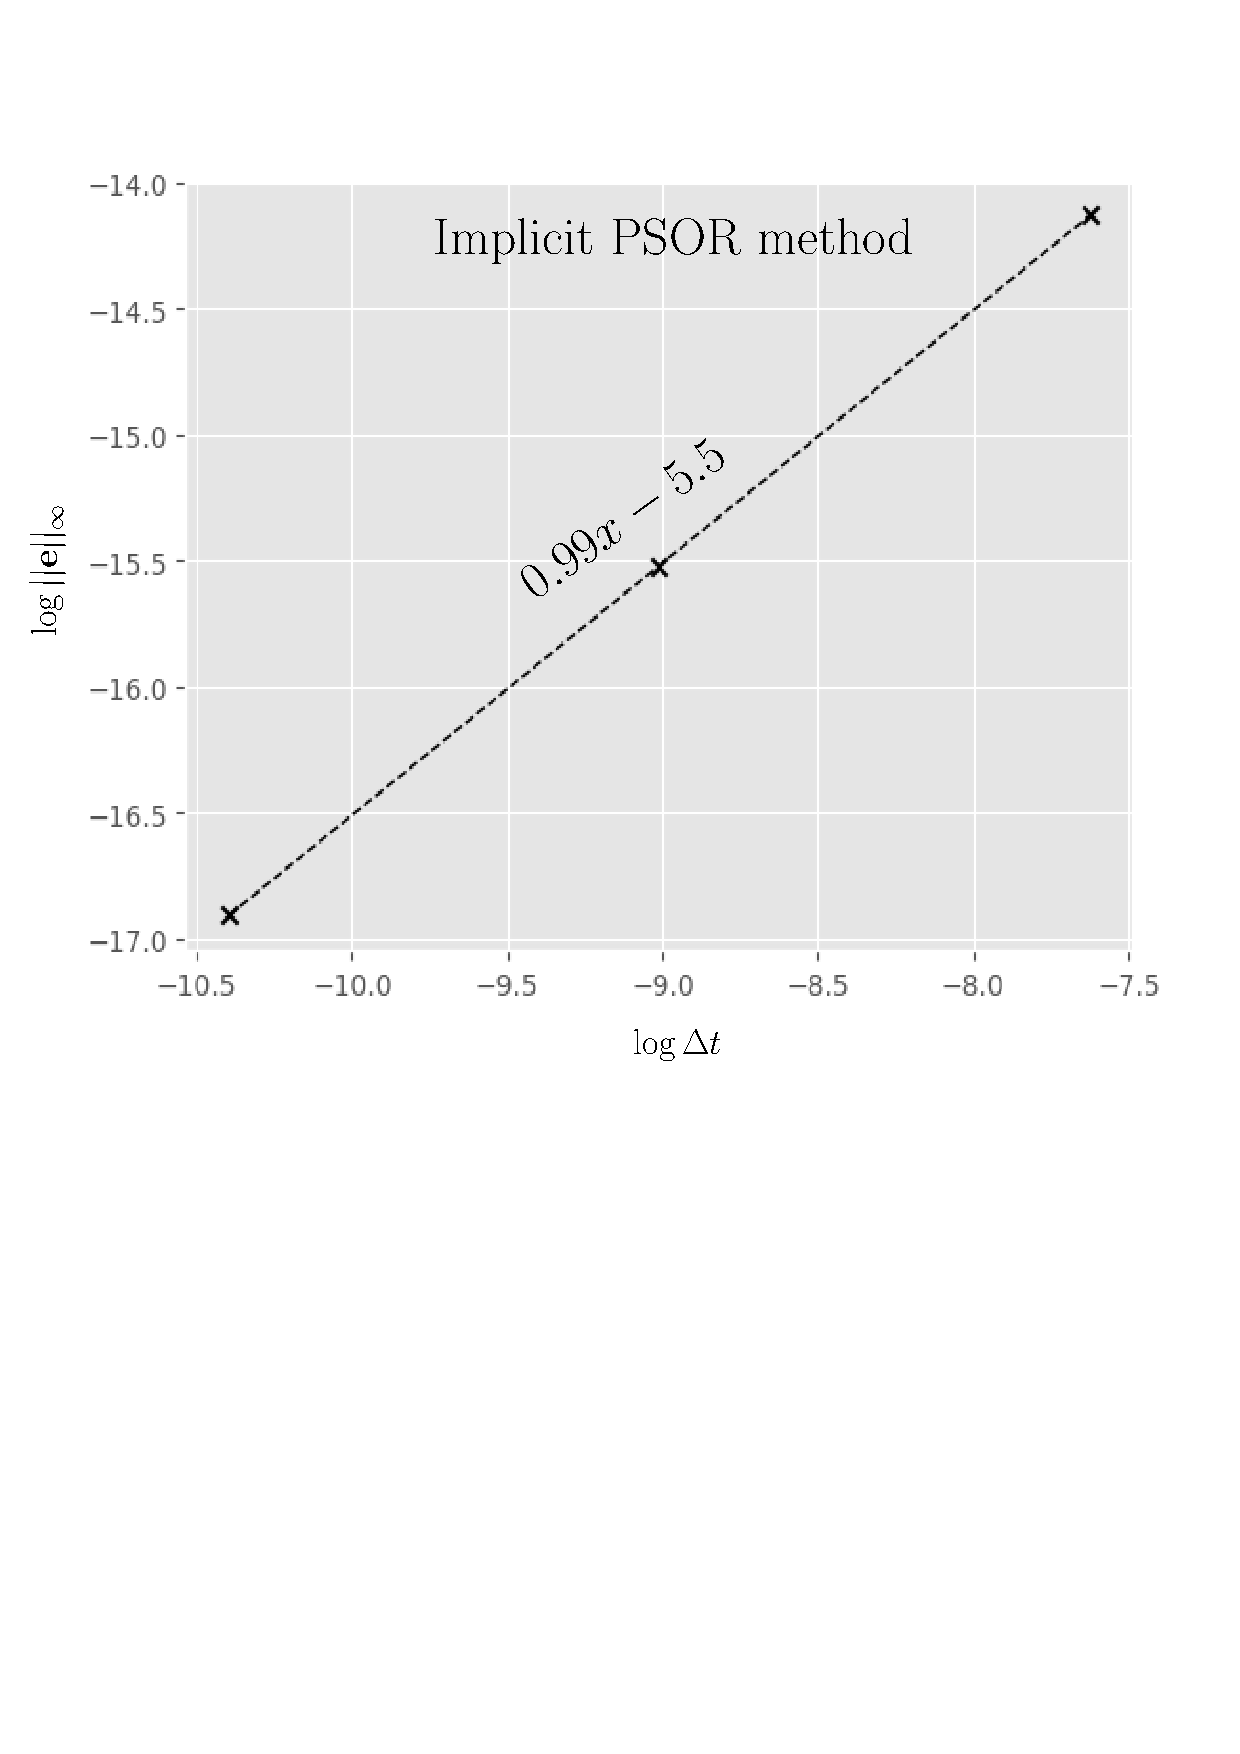
\includegraphics[width=\textwidth]{chapters/chapter5/ConvergenceTimeImplicitLCP.pdf}
    \caption{$\Delta{t}=2^{-15},2^{-17},\dots,2^{-21}$}
    \caption*{$\Delta{x}=2^{-7}$}
    \label{fig:lcp:numericalresults:convergence_time_implicit}
  \end{subfigure}
  \caption{Convergence analysis for the explicit method for the Company transformation.}
  \label{fig:lcp:numericalresults:implicit_convergence_analysis}
\end{figure}

\begin{figure}[tbp]
  \centering
  \begin{subfigure}{0.4\textwidth}
    \centering
    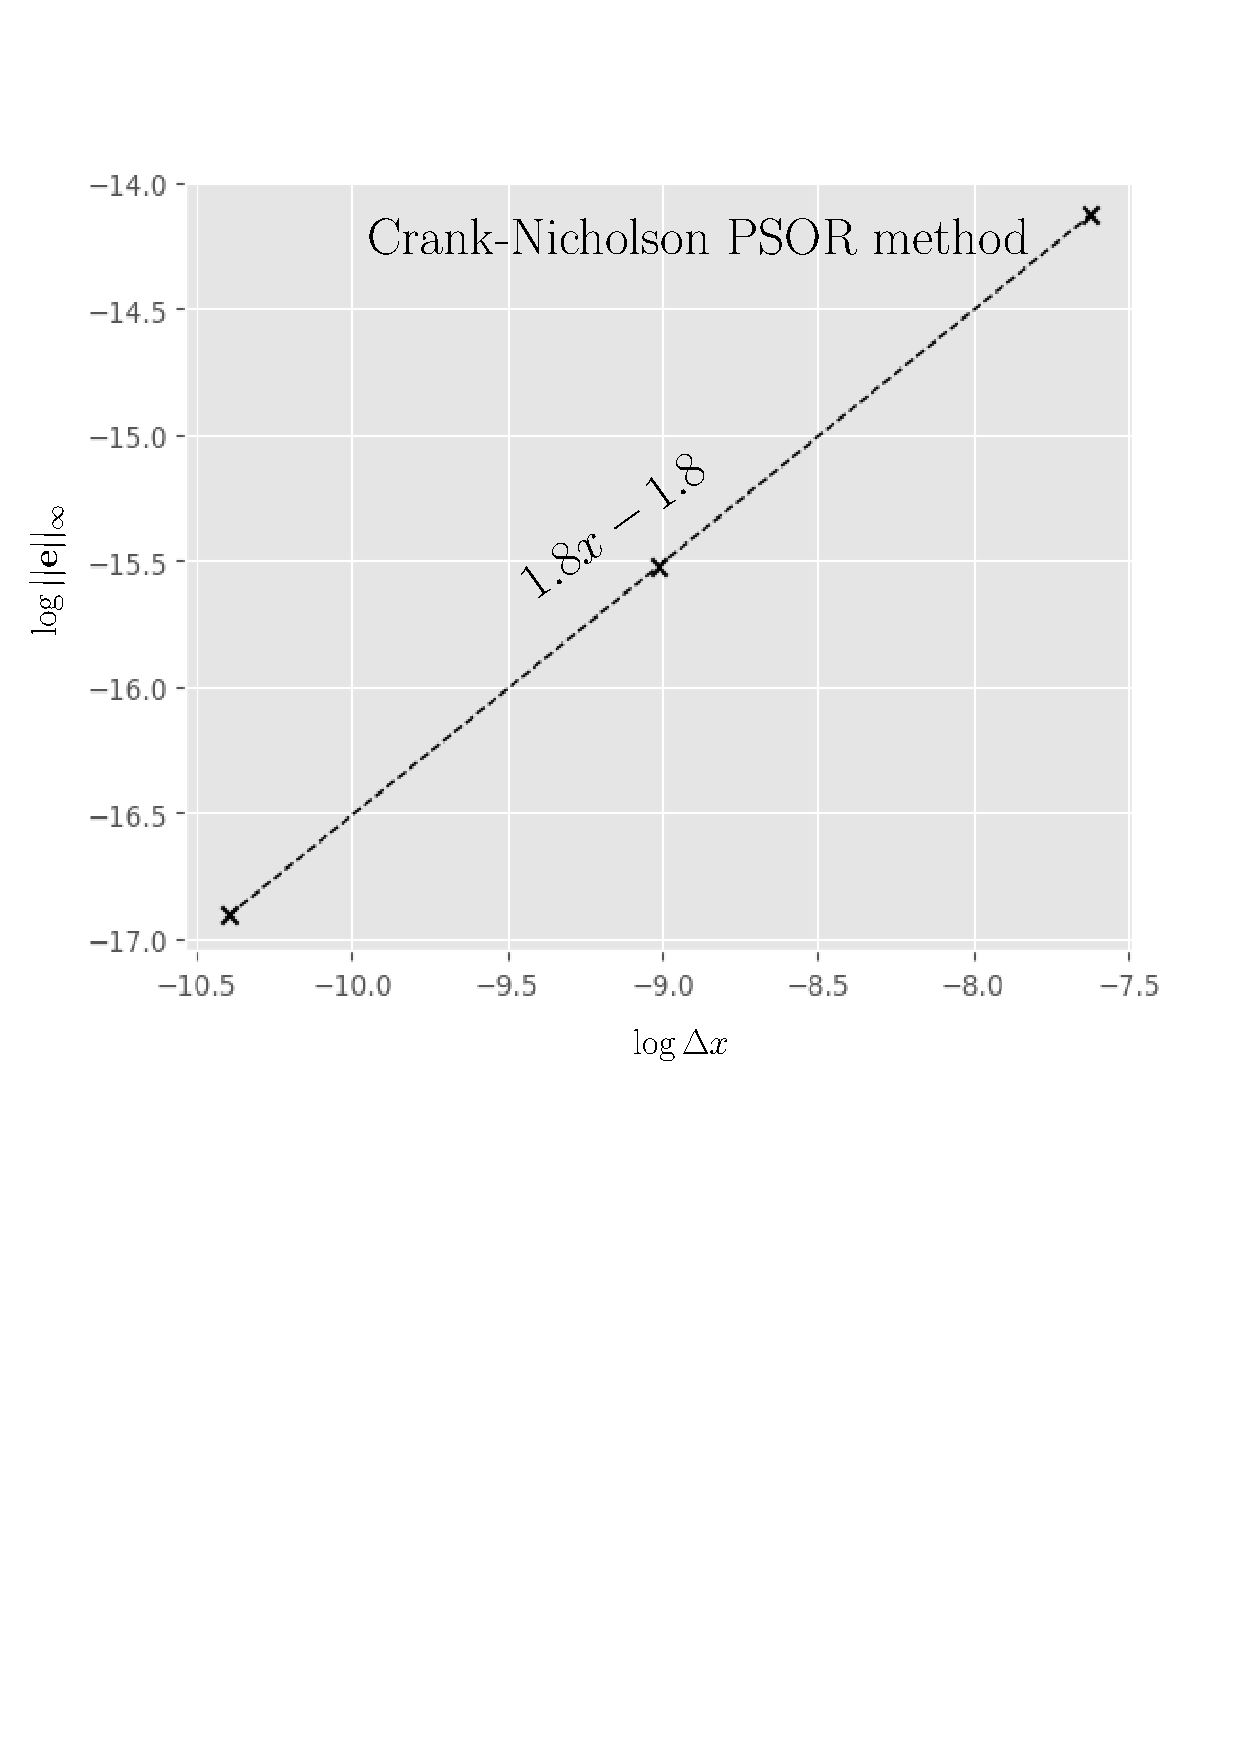
\includegraphics[width=\textwidth]{chapters/chapter5/ConvergenceSpaceCrankNicholsonLCP.pdf}
    \caption{$\Delta{x}=2^{-7},\dots,2^{-10}$}
    \caption*{$\Delta{t}=2^{-21}$}
    \label{fig:lcp:numericalresults:convergence_space_cranknicholson}
  \end{subfigure}
  \hspace{0.5cm}
  \begin{subfigure}{0.4\textwidth}
    \centering
    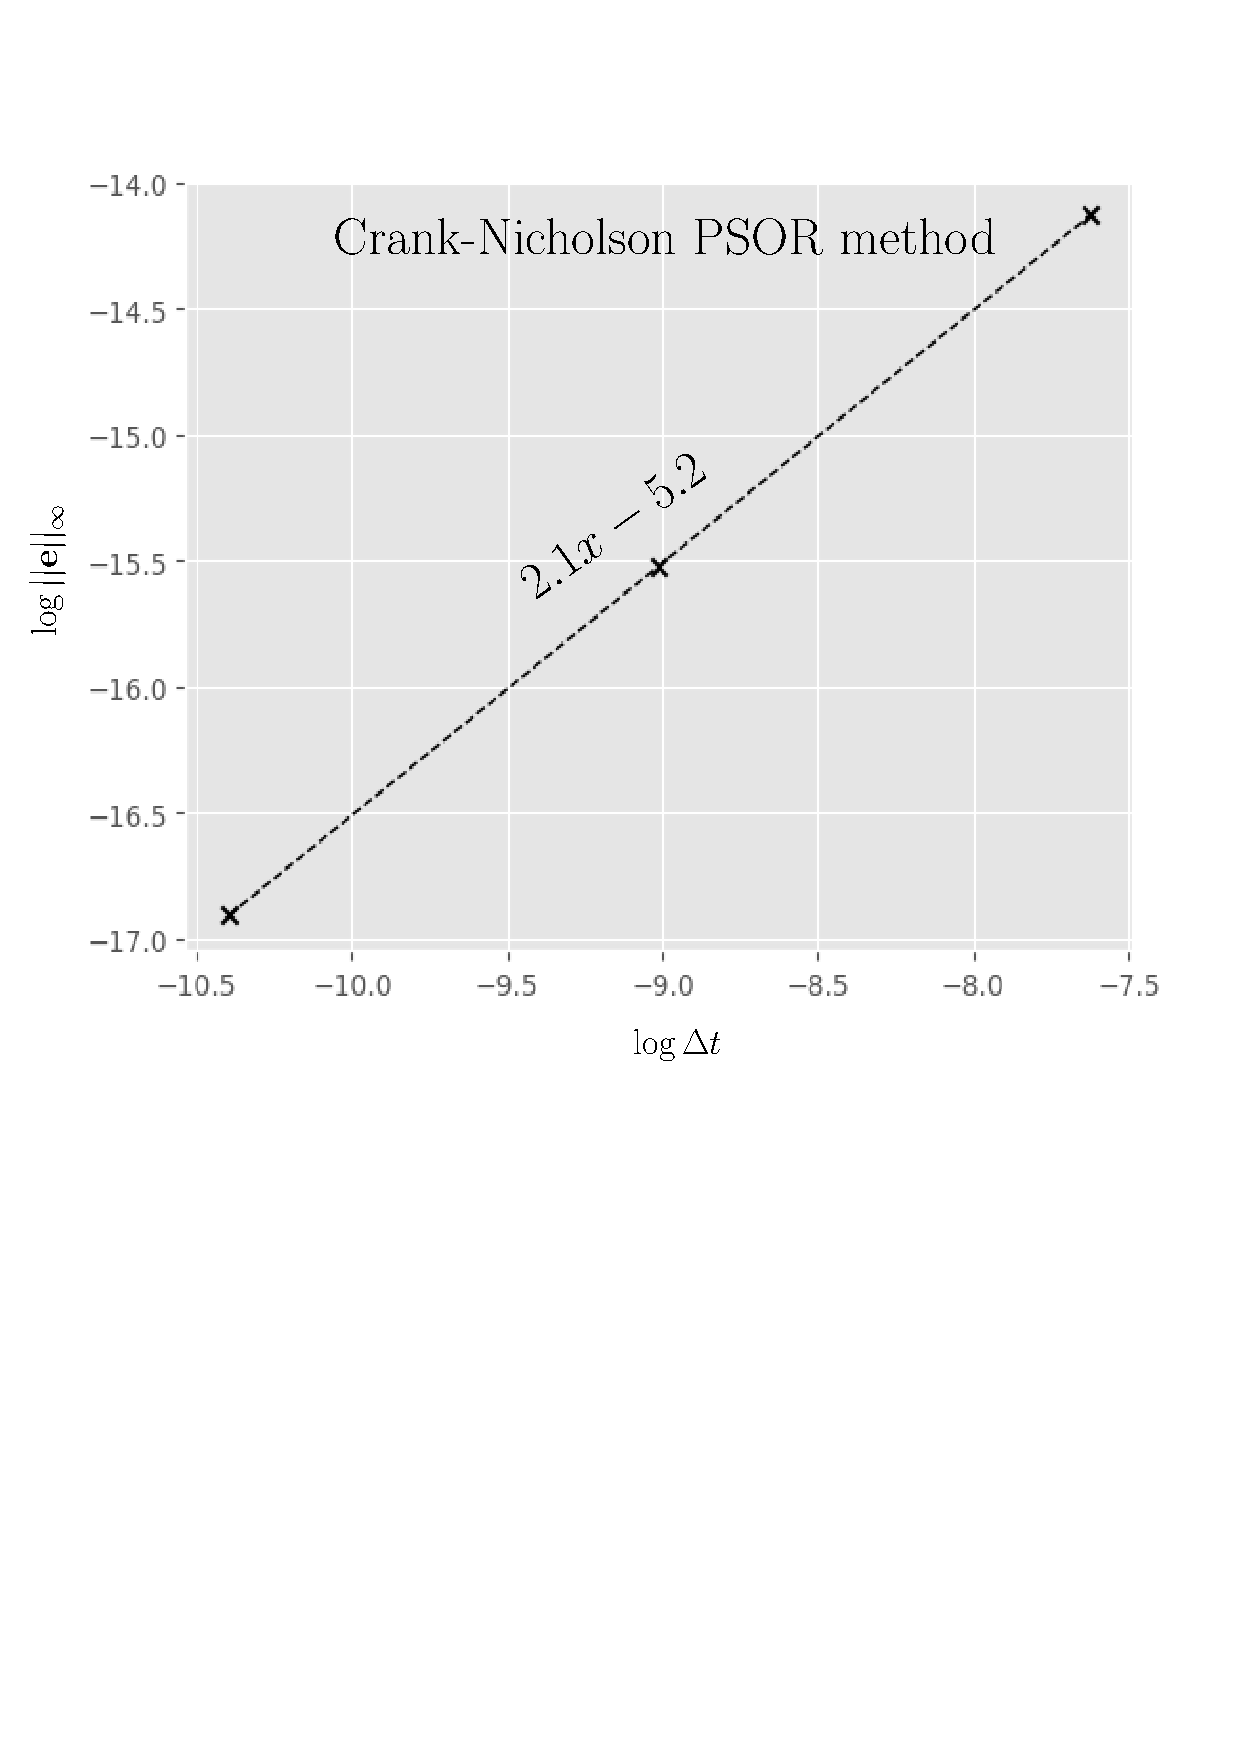
\includegraphics[width=\textwidth]{chapters/chapter5/ConvergenceTimeCrankNicholsonLCP.pdf}
    \caption{$\Delta{t}=2^{-15},2^{-17},\dots,2^{-21}$}
    \caption*{$\Delta{x}=2^{-7}$}
    \label{fig:lcp:numericalresults:convergence_time_cranknicholson}
  \end{subfigure}
  \caption{Convergence analysis for the explicit method for the Company transformation.}
  \label{fig:lcp:numericalresults:cranknicholson_convergence_analysis}
\end{figure}
\section{Conclusions}

An option provides the right to buy or sell an asset at a predetermined strike price in the future. Generally, investment firms are responsible for writing these contracts and selling them to investors. Subsequently, investors hold these contracts to hedge against potential changes in price. When a holder already owns an asset and wants to hedge against a potential price drop, they enter into a put option. On the contrary, if a holder aims to hedge against an increase in the price of an asset they intend to acquire, they enter into a call option contract. A wide variety of options are available in the market. Among the most notorious contracts, we have European and American options. European options are contracts that can exercise at the expiration date only. Likewise, American options are contracts that can be exercised before or at the maturity date. 

Investment firms charge premiums to investors for entering an option contract. Then, the writer uses the premium to hedge the possible claims that the holder will have in the future. Charging the correct premium is important because it minimizes the arbitrage opportunities for either the holder and writer. Clearly, pricing schemes depend on the type of the contract. In general, The Black-Scholes formula is used to price European options. Sadly, no formula is available for American options. Therefore, firms rely on numerical methods to come up with some approximation of the price. Numerous numerical methods for pricing American options derive from the Black-Scholes PDE. 

In this report we have implemented, and analyzed numerical schemes derived from the free boundary and the variational inequalities' formulation of the pricing problem. Specifically, we have discussed: An explicit and implicit front fixing schemes for solving the free boundary problem based on the Nielsen transformation, an explicit front fixing scheme based on the Company transformation, and the explicit, implicit and Crank-Nicholson PSOR schemes.

The explicit front fixing schemes were derived from applying central finite difference and forward/backward difference. However, they differ in how the contact point condition is approximated. Specifically, The Nielsen front fixing schemes use forward difference (or backward difference for call options) to approximate the contact point condition while the Company explicit scheme use central finite difference. This explains why Nielsen front fixing schemes yielded first order convergence with respect to the spatial discretization parameter $\Delta{x}$ while Company explicit scheme yielded second order. Moreover, as it is normally the case for explicit and implicit central finite differences, both Nielsen and Company schemes exhibits first order convergence with respect to the temporal discretization parameter $\Delta{t}$. While the explicit front fixing schemes for Nielsen and Company transformation are conditionally stable, they both proved to be substantially faster and much more accurate than the implicit scheme. 

We discourage the use of the Nielsen implicit scheme. As we already told, the implicit scheme is less accurate by far. The reason behind this is that the implicit scheme requires to solve a nonlinear system of equation at each time step in the grid. Moreover, the approximation errors produced by the nonlinear solver get accumulated over time, affecting the overall accuracy of the method. We could decrease the approximation error in the nonlinear solver by decreasing its tolerance, and increasing its maximum number of iteration. However, we found that as we do that, the overall performance of the method reduces substantially. To make things even worse, the size of the nonlinear equations is inversely proportional to the spatial discretization parameter. Therefore, the computational resources required by the implicit method grows substantially as we decrease the spatial discretization parameters. For instance, for a grid of $M$ nodes in the spatial direction, the non-linear solver needs to invert a Jacobian matrix of $M\times M$ entries. In other words, decreasing the spatial discretization parameters by a decimal point, requires 100 times more memory. To summarize, we can increase the accuracy of implicit method by decreasing the tolerance of the non-linear solver and by decreasing the discretization parameters of the grid but by sacrificing the performance of the method and increasing the memory consumption substantially.

Similar to the Company front fixing schemes, the PSOR schemes showed to have second order convergence with respect to the spatial discretization parameter $\Delta{x}$. Moreover, it showed to have first order convergence for the explicit ($\theta=0$) and implicit ($\theta=1$) schemes, and second order convergence for the Crank-Nicholson ($\theta=0.5$) in with respect to the temporal discretization parameter $\Delta{t}$. Analogous to the explicit front fixing schemes, the PSOR explicit scheme is conditionally stable. When comparing the performance of the explicit PSOR to the explicit front fixing schemes, the explicit front fixing schemes showed to be substantially faster. In that regard, the issue with explicit PSOR is that as you decrease $\Delta{x}$, the complementary equations grow, hence, taking more time to solve the linear complementary problem. Similar argument can be done when comparing explicit front fixing schemes to the implicit and Crank-Nicholson PSOR schemes. In spite of that, the Crank-Nicholson PSOR scheme is second order convergence in time, therefore, by choosing $\Delta{x}$ to be smaller than $\Delta{t}$, we could have greater performance maintaining the accuracy. 

Concluding, the numerical experiments conducted showed that the explicit front-fixing schemes offers superior performance and accuracy than the implicit front fixing scheme and the all the PSOR schemes. Between the Company explicit front fixing scheme and the Nielsen explicit front fixing scheme, we recommend using the Company transformation because it has second order convergence in space, hence, yielding to smaller approximation errors. Similarly, the explicit PSOR scheme exhibited smaller approximation errors and computational than the implicit and Crank-Nicholson PSOR schemes and the implicit front fixing scheme. However, it is still rather slow compared to the explicit front fixing schemes.

\section{Further research}

Further research opportunities arise from this report. Firstly, we saw that generally, people transform the Black-Scholes PDE to the heat diffusion equation. Although this was done for the LCP problem, the front fixing schemes derived within the option's domain which might led to worse approximations or slower performance. Moreover, we might derive Nielsen front fixing scheme that approximates the contact point condition using central finite differences. Likewise, for the Nielsen implicit front fixing scheme, we could explore using nonlinear methods for large scale-scale nonlinear systems such as the one proposed by\cite{lacruz_2006}. Also, we might derive Crank-Nicholson schemes for the Nielsen and Company front fixing schemes. Finally, we might consider using real market data to evaluate how good are the numerical schemes presented under real market conditions.

% \section{Front fixing method}

\subsection{Inverse transformation}

\begin{equation}
    \frac{\partial{V}}{\partial{t}} + \frac{1}{2}\sigma^{2} S^2 \frac{\partial^2{V}}{\partial{S^2}} + (r - \delta) S \frac{\partial{V}}{\partial{S}} - rV = 0 \quad \text{for $S > \bar{S}(t)$ and $0 \le t < T$}
\end{equation}

\begin{equation}
    V(S, t) = K - S \quad  \text{for $0 \le S \le \bar{S}(t)$ and $0 \le t < T$}
\end{equation}

\begin{equation}
    V(S, T) = \max(K - S, 0) \quad \text{for $S \ge 0$}
\end{equation}

\begin{equation}
    \frac{\partial{V}}{\partial{S}}(\bar{S}(t), t) = -1
\end{equation}

\begin{equation}
    \lim_{S\rightarrow \infty} V(S, t) = 0
\end{equation}

\begin{equation}
    \bar{S}(T) = K
\end{equation}

In order for remove the free boundary in the system of equation, the following 
transformation is used:

\begin{equation}
    x = \frac{S}{\bar{S}(t)}
\end{equation}

Next,

\begin{equation}
    v(x, t) := V(x\bar{S}(t), t) = V(S, t)
\end{equation}


By computing the partial derivatives of V with respect to S and t

\begin{equation}
    \frac{\partial{V}}{\partial{t}} =  \frac{\partial{v}}{\partial{t}} + \frac{\partial{v}}{\partial{x}} \frac{\partial{x}}{\partial{t}} 
    = \frac{\partial{v}}{\partial{t}} - x\frac{\bar{S}^\prime(t)}{\bar{S}(t)}\frac{\partial{v}}{\partial{x}} 
\end{equation}

\begin{equation}
    \frac{\partial{V}}{\partial{S}} = \frac{\partial{v}}{\partial{x}} 
    \frac{\partial{x}}{\partial{S}} = 
    \frac{1}{\bar{S}(t)} \frac{\partial{v}}{\partial{x}}
\end{equation}

\begin{equation}
    \frac{\partial^2{V}}{\partial{S^2}} =
    \frac{1}{\bar{S}(t)^2} \frac{\partial^2{v}}{\partial{x}^2}
\end{equation}

an expression for (3.1) with respect to $x$ is derived:

\begin{equation}
    \frac{\partial{v}}{\partial{t}} + \frac{1}{2}\sigma^{2} x^2 \frac{\partial^2{v}}{\partial{x}^2} + \bigg[(r - \delta) - \frac{\bar{S}^\prime(t)}{\bar{S}(t)}\bigg]x\frac{\partial{v}}{\partial{x}} - rv = 0 \quad \text{for $x > 1$ and $0 \le t < T$}
\end{equation}

Similarly, (3.2) is reformulated in term of x to:

\begin{equation}
    v(x, t) = K - x\bar{S}(t) \quad  \text{for $0 \le x \le 1$ and $0 \le t < T$}
\end{equation}

Next, the terminal condition (3.3) is re-written with respect of x:

\begin{equation}
    v(x, T) = \max(K - x\bar{S}(T), 0) = K \max(1 - x, 0) = 0 \quad \text{for $x \ge 1$}
\end{equation}

Finally, the left and right boundary conditions are given with respect to x:

\begin{equation}
    \frac{\partial{v}}{\partial{x}}(x, t) = -\bar{S}(t)
\end{equation}

\begin{equation}
    \lim_{x \rightarrow \infty} v(x, t) = 0
\end{equation}

In summary, a non linear system of PDEs is obtained:

\begin{equation}
    \frac{\partial{v}}{\partial{t}} + \frac{1}{2}\sigma^{2} x^2 \frac{\partial^2{v}}{\partial{x}^2} + \bigg[(r - \delta) - \frac{\bar{S}^\prime(t)}{\bar{S}(t)}\bigg]x\frac{\partial{v}}{\partial{x}} - rv = 0 \quad \text{for $x > 1$ and $0 \le t < T$}
\end{equation}

\begin{equation}
    v(x, t) = K - x\bar{S}(t) \quad  \text{for $0 \le x \le 1$ and $0 \le t < T$}
\end{equation}

\begin{equation}
    v(x, T) = 0 \quad \text{for $x \ge 1$}
\end{equation}

\begin{equation}
    \frac{\partial{v}}{\partial{x}}(x, t) = -\bar{S}(t)
\end{equation}

\begin{equation}
    \lim_{x \rightarrow \infty} v(x, t) = 0
\end{equation}

\begin{equation}
    \bar{S}(T) = K
\end{equation}
\newpage

\appendix


\section{Explicit scheme for Company transformation} 
The explicit scheme is given by
\begin{equation*}
    \begin{split}
      \dfrac{v^{n+1}_{i} - v^{n}_{i}}{\Delta{t}} & - \dfrac{1}{2}\sigma^2 \dfrac{v^{n}_{i-1} - 2v^{n}_{i} + v^{n}_{i+1}}{(\Delta{x})^2} \\ 
       & - \bigg( (r-\delta) - \dfrac{\sigma^2}{2} - \dfrac{\bar{S}^{n+1}_{f} - \bar{S}^{n}_{f}}{\Delta{t}\bar{S}^{n}_{f}} \bigg)\dfrac{v^{n}_{i+1} - v^{n}_{i-1}}{2\Delta{x}} + rv^{n}_{i} = 0
    \end{split}
\end{equation*}
for $i=1\dots,M$ and $n = 0,\dots,N$. 
\begin{equation*}
    \begin{split}
        v^{n+1}_{i} = av^{n}_{i-1} + bv^{n}_{i} + cv^{n}_{i+1} + \dfrac{\bar{S}^{n+1}_{f} - \bar{S}^{n}_{f}}{2\Delta{x}\bar{S}^{n}_{f}}(v^{n}_{i+1} - v^{n}_{i-1})
    \end{split}
\end{equation*}
where 
\begin{equation*}
    \begin{split}
        \lambda =& \dfrac{\Delta{t}}{\Delta{x}^2}\\
        a =& \dfrac{\lambda}{2}\bigg( \sigma^2 - \bigg(r - \delta - \dfrac{\sigma^2}{2}\bigg)\Delta{x} \bigg) \\
        b =& 1 - \sigma^2\lambda- r\Delta{t} \\
        c =& \dfrac{\lambda}{2}\bigg(\sigma^2 + \bigg(r - \delta - \dfrac{\sigma^2}{2}\bigg)\Delta{x}\bigg)
    \end{split}
\end{equation*}
Moreover, the boundary conditions 
\begin{equation*}
    \begin{split}
        \text{\textbf{Call:}} \qquad & v^{n}_{0} = 0, \quad v^{n}_{M+1} = \bar{S}^{n}_{f} - 1 \\
        \text{\textbf{Put:}} \qquad & v^{n}_{0} = 1 - \bar{S}^{n}_{f}, \quad v^{n}_{M+1} = 0 \\
    \end{split}
\end{equation*}
for $n=0,\dots,N$. Moreover, the contact point condition is approximated using central finite difference
\begin{align*}
    \text{\textbf{Call:}} \qquad & \dfrac{v^{n}_{M+2} - v^{n}_{M}}{2\Delta{x}^2} = \dfrac{\partial{v}}{\partial{x}}(0, t) + O(\Delta{x}^2) \\
    \text{\textbf{Put:}} \qquad & \dfrac{v^{n}_{1} - v^{n}_{-1}}{2\Delta{x}} = \dfrac{\partial{v}}{\partial{x}}(0, t)+ O(\Delta{x}^2) 
\end{align*}

for $n=0,\dots,N$. Moreover, the contact point condition is approximated using central finite difference
\begin{align}
    \label{eq:appendix:explicitmethodcompany:contact_point_approximation}
    \text{\textbf{Call:}} \qquad & \dfrac{v^{n}_{M+2} - v^{n}_{M}}{2\Delta{x}^2} = \bar{S}^{n}_{f} \\
    \text{\textbf{Put:}} \qquad & \dfrac{v^{n}_{1} - v^{n}_{-1}}{2\Delta{x}}  = -\bar{S}^{n}_{f}  
\end{align}

By combining the central difference approximation for the PDE, the boundary conditions and the contact point, it is obtained 

\begin{align*}
    \text{\textbf{Call:}} \qquad & v^{n}_{M} =  \\
    \text{\textbf{Put:}} \qquad & v^{n}_{1} = \alpha - \beta\bar{S}^{n}_{f}  
\end{align*}

\begin{algorithm}[H]
    \caption{Explicit method for put options}\label{alg:appendix:companytransformation:explicits:put_explicit_method_algorithm}
    \begin{algorithmic}
    \For{$i = 0,\dots,M+1$} 
      \State $v^{0}_i = 0 $
    \EndFor
    \State $\bar{S}_{f}^{0} = K$

    \State $a = \dfrac{\lambda}{2}\bigg(\sigma^2 - \bigg(r - \delta - \dfrac{\sigma^2}{2}\bigg)\Delta{x}\bigg)$
    \State $b = 1 - \sigma^2\lambda- r\Delta{t} $
    \State $c = \dfrac{\lambda}{2}\bigg(\sigma^2 + \bigg(r - \delta - \dfrac{\sigma^2}{2}\bigg)\Delta{x}\bigg)$
    \State $\alpha = 1 + \dfrac{r\Delta{x}^2}{\sigma^2}$
    \State $\beta = 1 + \Delta{x} + \dfrac{1}{2}\Delta{x}^2$

    \For{$n = 0, \dots, N$}
      \State $d^n = \dfrac{\alpha - (av^{n}_{0} + bv^{0}_{1} + cv^{n}_{2} - (v^{n}_{2} - v^{n}_{0})/(2\Delta{x}))}{(v^{n}_{2} - v^{n}_{0})/(2\Delta{x}) + \beta\bar{S}^{n}_f}$
      \State $\bar{S}^{n+1}_{f}=d^{n}\bar{S}^{n}_{f}$
      \State $a^{n} = a - \dfrac{\bar{S}^{n+1}_{f} - \bar{S}^{n}_{f}}{2\Delta{x}\bar{S}^{n}_{f}}$
      \State $c^{n} = c - \dfrac{\bar{S}^{n+1} - \bar{S}^{n}}{2\Delta{x}\bar{S}^{n}_{f}}$

      \State $v^{n+1}_{0}=1 - \bar{S}^{n+1}_{f}$
      \State $v^{n+1}_{1}=\alpha - \beta\bar{S}^{n+1}_{f}$
      \State $v^{n+1}_{M+1} = 0$
      \For{$i = 2, \dots, M$}
        \State $v^{n+1}_{i} = a^{n} v^{n}_{i-1} + b v^{n}_{i} + c^{n}v^{n}_{i+1}$
      \EndFor
    \EndFor
  \end{algorithmic}
  \end{algorithm}
\section{Python implementation}
The following python code is simplified version of the final implementation. A complete version can be found at \url{https://github.com/Alcruz/math4062-dissertation}.

\begin{lstlisting}[language=Python, caption=Base classses for options solver.]
    class Option(ABC):
        def __init__(self, type: OptionType, K: float, T: float):
            self.type = type
            self.K = K # Strike price
            self.T = T # Maturity

        @abstractmethod
        def payoff(self, S: float):
            pass
    class CallOption(Option):
        def __init__(self, K: float, T: float):
            super().__init__(OptionType.CALL, K, T)
        def payoff(self, S: float):
            return np.maximum(S - self.K, 0) 
    class PutOption(Option):
        def __init__(self, K: float, T: float):
            super().__init__(OptionType.PUT, K, T)
        def payoff(self, S: float):
            return np.maximum(self.K - S, 0)
    class Solver(ABC): 
        def __init__(self, 
            option: Option,
            r: float,  # risk-free interest rate
            sigma: float,  # sigma price volatitliy
            dx: float,  # grid resolution along x-axis
            dt: float,  # grid resolution along t-axis
            delta # dividends
        ) -> None:
            self.option = option
            self.r = r
            self.sigma = sigma
            self.dx = dx
            self.dt = dt
            self.delta = delta
\end{lstlisting}
\begin{lstlisting}[language=Python, caption=Explicit solver for Nielsen transformation.]
    class ExplicitSolver(Solver):
        def __init__(self, 
            option: Option,
            r: float,  # risk-free interest rate
            sigma: float,  # sigma price volatitliy
            dx: float,  # grid resolution along x-axis
            dt: float,  # grid resolution along t-axis
            delta # dividends
        ) -> None:
            self.option = option
            self.r = r
            self.sigma = sigma
            self.dx = dx
            self.dt = dt
            self.delta = delta
            lambd = dt / np.power(dx, 2)
            alpha = dt / dx
            self.A = 0.5 * np.power(sigma*self.x_axis, 2) * lambd - 0.5 * self.x_axis * ((r-delta) - (1/dt)) * alpha
            self.B = 1 - np.power(sigma*self.x_axis, 2) * lambd - r*dt
            self.C = 0.5 * np.power(sigma*self.x_axis, 2) * lambd + 0.5 * self.x_axis * ((r-delta) - (1/dt)) * alpha
        def solve(self):
            V = np.zeros_like(self.x_axis)
            S_bar = self.option.K
            for _ in np.arange(0, self.option.T, self.dt):
                D = 0.5*self.x_axis/self.dx
                D[1:-1] *= (V[2:]-V[:-2]) * (1/S_bar)
                
                S_bar = self.compute_time_iteration(V, D)
            return S_bar*self.x_axis, V, S_bar
        @abstractmethod
        def compute_time_iteration(self, V: np.ndarray, D: np.ndarray):
            pass
    class CallOptionExplicitSolver(ExplicitSolver):
        def __init__(self, 
            option: CallOption,
            r: float,  # risk-free interest rate
            sigma: float,  # sigma price volatitliy
            dx: float,  # grid resolution along x-axis
            dt: float,  # grid resolution along t-axis
            delta=0  # dividends
        ):
            self.x_axis = np.arange(0, 1+dx, dx)
            super().__init__(option, r, sigma, dx, dt, delta)
        def compute_time_iteration(self, V: np.ndarray, D: np.ndarray):
            S_bar = self.option.K + self.A[-2]*V[-3] + self.B[-2]*V[-2] + self.C[-2]*V[-1]
            S_bar /= 1 - self.dx - D[-2]
    
            V[1:-2] = self.A[1:-2]*V[:-3] + self.B[1:-2]*V[1:-2] \
                + self.C[1:-2]*V[2:-1] + D[1:-2]*S_bar
            V[-2] = (1-self.dx)*S_bar - self.option.K
            V[-1] = S_bar - self.option.K
            return S_bar
    class PutOptionExplicitSolver(ExplicitSolver):
        def __init__(self, 
            option: PutOption,
            r: float,  # risk-free interest rate
            sigma: float,  # sigma price volatitliy
            dx: float,  # grid resolution along x-axis
            dt: float,  # grid resolution along t-axis
            x_max: 2.,  # sufficiently large value for x
            delta=0  # dividends
        ):
            self.x_axis = np.arange(1, x_max+dx, dx)
            super().__init__(option, r, sigma, dx, dt, delta)
        def compute_time_iteration(self, V: np.ndarray, D: np.ndarray) -> float:
            S_bar = self.option.K - (self.A[1]*V[0] + self.B[1]*V[1] + self.C[1]*V[2])
            S_bar /= D[1] + 1 + self.dx
            V[2:-1] = self.A[2:-1]*V[1:-2] + self.B[2:-1] * \
                V[2:-1] + self.C[2:-1]*V[3:] + D[2:-1]*S_bar
            V[0] = self.option.payoff(S_bar)
            V[1] = self.option.payoff((1+self.dx)*S_bar)
            return S_bar
\end{lstlisting}

\begin{lstlisting}[language=Python, caption=Implicit solver for Nielsen transformation]
    class ImplicitSolver(Solver):
        def __init__(self, 
            option: Option,
            r: float,  # risk-free interest rate
            sigma: float,  # sigma price volatitliy
            dx: float,  # grid resolution along x-axis
            dt: float,  # grid resolution along t-axis
            delta=0, # dividends
        ) -> None:
            self.option = option
            self.r = r
            self.sigma = sigma
            self.dx = dx
            self.dt = dt
            self.delta = delta
            self.lambd = self.dt/np.power(self.dx, 2)
            self.kappa = self.dt/self.dx
            self.alpha = 1 + self.lambd*np.power(self.sigma*self.x_axis, 2) + self.r*self.dt
            self.M = self.x_axis.size 
        def beta(self, S, S_bar):
            return -0.5*self.lambd*np.power(self.sigma, 2)*np.power(self.x_axis, 2) + 0.5*self.kappa*self.x_axis*((self.r-self.delta) - (S_bar - S)/(self.dt*S))
        def gamma(self, S, S_bar):
            return -0.5*self.lambd*np.power(self.sigma, 2)*np.power(self.x_axis, 2) - 0.5*self.kappa*self.x_axis*((self.r-self.delta) - (S_bar - S)/(self.dt*S))
        @abstractmethod
        def solve_non_linear_system(self, V, S_bar) -> float:
            pass
        def solve(self):
            S_bar = self.option.K
            V = np.zeros_like(self.x_axis)
            for _ in np.arange(0, self.option.T, self.dt):
                S_bar = self.solve_non_linear_system(V, S_bar)
            return S_bar*self.x_axis, V, S_bar
    class CallOptionImplicitSolver(ImplicitSolver):
        def __init__(self, 
            option: Option,
            r: float,  # risk-free interest rate
            sigma: float,  # sigma price volatitliy
            dx: float,  # grid resolution along x-axis
            dt: float,  # grid resolution along t-axis
            delta=0, #dividends
            maxiter=1000,
            tolerance=1e-24,
            method='lm'
        ) -> None:
            self.x_axis = np.arange(0, 1+dx, dx)
            super().__init__(option, r, sigma, dx, dt, delta)
            self.maxiter=maxiter
            self.tolerance=tolerance
            self.method=method
        def jacobian(self, y, S_bar):
            p, s, = y[:-1], y[-1]
            beta = self.beta(s, S_bar)
            gamma = self.gamma(s, S_bar)
            dgamma_ds = - 0.5 * (1/self.dx) * self.x_axis * S_bar / s**2
            dbeta_ds = 0.5 * (1/self.dx) * self.x_axis * S_bar / s**2
            retVal = diags([self.alpha[2:], beta[1:-1], gamma[1:-1]],
                        [-1, 0, 1], shape=(self.M-2, self.M-2)).toarray()
            retVal[-1, :] = 0
            retVal[:, -1] = 0
            retVal[0, -1] = dbeta_ds[1]*p[0] + dgamma_ds[1]*p[1]
            retVal[1:-2, -1] = dbeta_ds[2:-3]*p[1:-1] + dgamma_ds[2:-3]*p[2:]
            retVal[-2, -1] = dbeta_ds[-3]*p[-2]
            retVal[-2, -1] -= dgamma_ds[-3]*self.option.payoff((1-self.dx)*s) + gamma[-3]*(1 - self.dx)
            retVal[-1, -2] = self.alpha[-2]
            retVal[-1, -1] -= dgamma_ds[-2]*self.option.payoff(s) + gamma[-2] + dbeta_ds[-2]*self.option.payoff((1-self.dx)*s) - beta[1]*(1-self.dx)
            return retVal
        def system(self, y, b, S_bar):
            *v, s = y
            beta = self.beta(s, S_bar)
            gamma = self.gamma(s, S_bar)
            A = diags([self.alpha[2:-1], beta[1:-2], gamma[1:-3]],
                    [-1, 0, 1], shape=(self.M-2, self.M-3)).toarray()
            f = b[1:-1]
            f[-2] -= gamma[-3]*((1-self.dx)*s-self.option.K)
            f[-1] -= gamma[-2]*(s-self.option.K) + beta[-2]*((1-self.dx)*s - self.option.K)
            res = A@v - f
            return res
        def solve_non_linear_system(self, V: np.ndarray, S_bar: np.ndarray):
            *V[1:-2], S_bar = root(
                lambda y: self.system(y, np.copy(V[:]), S_bar),
                # jac=lambda y: self.jacobian(y, S_bar),
                x0=np.concatenate([V[1:-2], [S_bar]]),
                method=self.method,
                options=dict(xtol=self.tolerance, maxiter=self.maxiter)
            )['x']
            V[-2] = (1-self.dx)*S_bar-self.option.K
            V[-1] = S_bar-self.option.K
            return S_bar
    class PutOptionImplicitSolver(ImplicitSolver):
        def __init__(self, 
            option: Option,
            r: float,  # risk-free interest rate
            sigma: float,  # sigma price volatitliy
            dx: float,  # grid resolution along x-axis
            dt: float,  # grid resolution along t-axis
            delta=0, # dividends
            x_max=2,
            maxiter=1000,
            tolerance=1e-24,
            method='lm'
        ) -> None:
            self.x_axis = np.arange(1, x_max+dx, dx)
            super().__init__(option, r, sigma, dx, dt, delta)
            self.maxiter=maxiter
            self.tolerance=tolerance
            self.method=method
        def jacobian(self, y, S_bar):
            p, s, = y[:-1], y[-1]
            beta = self.beta(s, S_bar)
            gamma = self.gamma(s, S_bar)
    
            dgamma_ds = - 0.5 * (1/self.dx) * self.x_axis * S_bar / s**2
            dbeta_ds = 0.5 * (1/self.dx) * self.x_axis * S_bar / s**2
    
            retVal = diags([beta[3:-1], self.alpha[2:-1], gamma[1:-1]],
                        [-2, -1, 0], shape=(self.M-2, self.M-2)).toarray()
            retVal[-1, :] = 0
            retVal[:, -1] = 0
            retVal[0, -1] = dgamma_ds[1]*p[0] + dbeta_ds[1] * \
                (self.option.K - S_bar) - beta[1] - self.alpha[1]*(1+self.dx)
            retVal[1, -1] = dgamma_ds[2]*p[1] + dbeta_ds[2] * \
                (self.option.K - (1+self.dx)*S_bar) - beta[2]*(1+self.dx)
            retVal[2:-1, -1] = dbeta_ds[3:-2]*p[:-2] + dgamma_ds[3:-2]*p[2:]
            retVal[-1, -3] = beta[-2]
            retVal[-1, -2] = self.alpha[-2]
            retVal[-1, -1] = dbeta_ds[-2]*p[-2]
            return retVal
        def system(self, y, b, S_bar):
            p, s, = y[:-1], y[-1]
            _beta = self.beta(s, S_bar)
            _gamma = self.gamma(s, S_bar)
            A = diags([_beta[3:-1], self.alpha[2:-1], _gamma[1:-2]],
                    [-2, -1, 0], shape=(self.M-2, self.M-3)).toarray()
            f = b[1:-1]
            f[0] -= _beta[1]*(self.option.K-s) + self.alpha[1]*((self.option.K-(1+self.dx)*s))
            f[1] -= _beta[2]*(self.option.K-(1+self.dx)*s)
            res = A@p - f
            return res
        def solve_non_linear_system(self, V: np.ndarray, S_bar: np.ndarray):
            *V[2:-1], S_bar = root(
                lambda y: self.system(y, np.copy(V[:]), S_bar),
                # jac=lambda y: self.jacobian(y, S_bar),
                x0=np.concatenate([V[2:-1], [S_bar]]),
                method=self.method,
                options=dict(xtol=self.tolerance, maxiter=self.maxiter)
            )['x']
            V[0] = self.option.payoff(S_bar)
            V[1] = self.option.payoff((1+self.dx)*S_bar)    
            return S_bar
\end{lstlisting}

\section{Code for numerical experiments} \label{sec:numericalexperiments}
% \section{Code for convergence analysis} \label{sec:convergenceanalysis}
% \vspace{2cm}
% 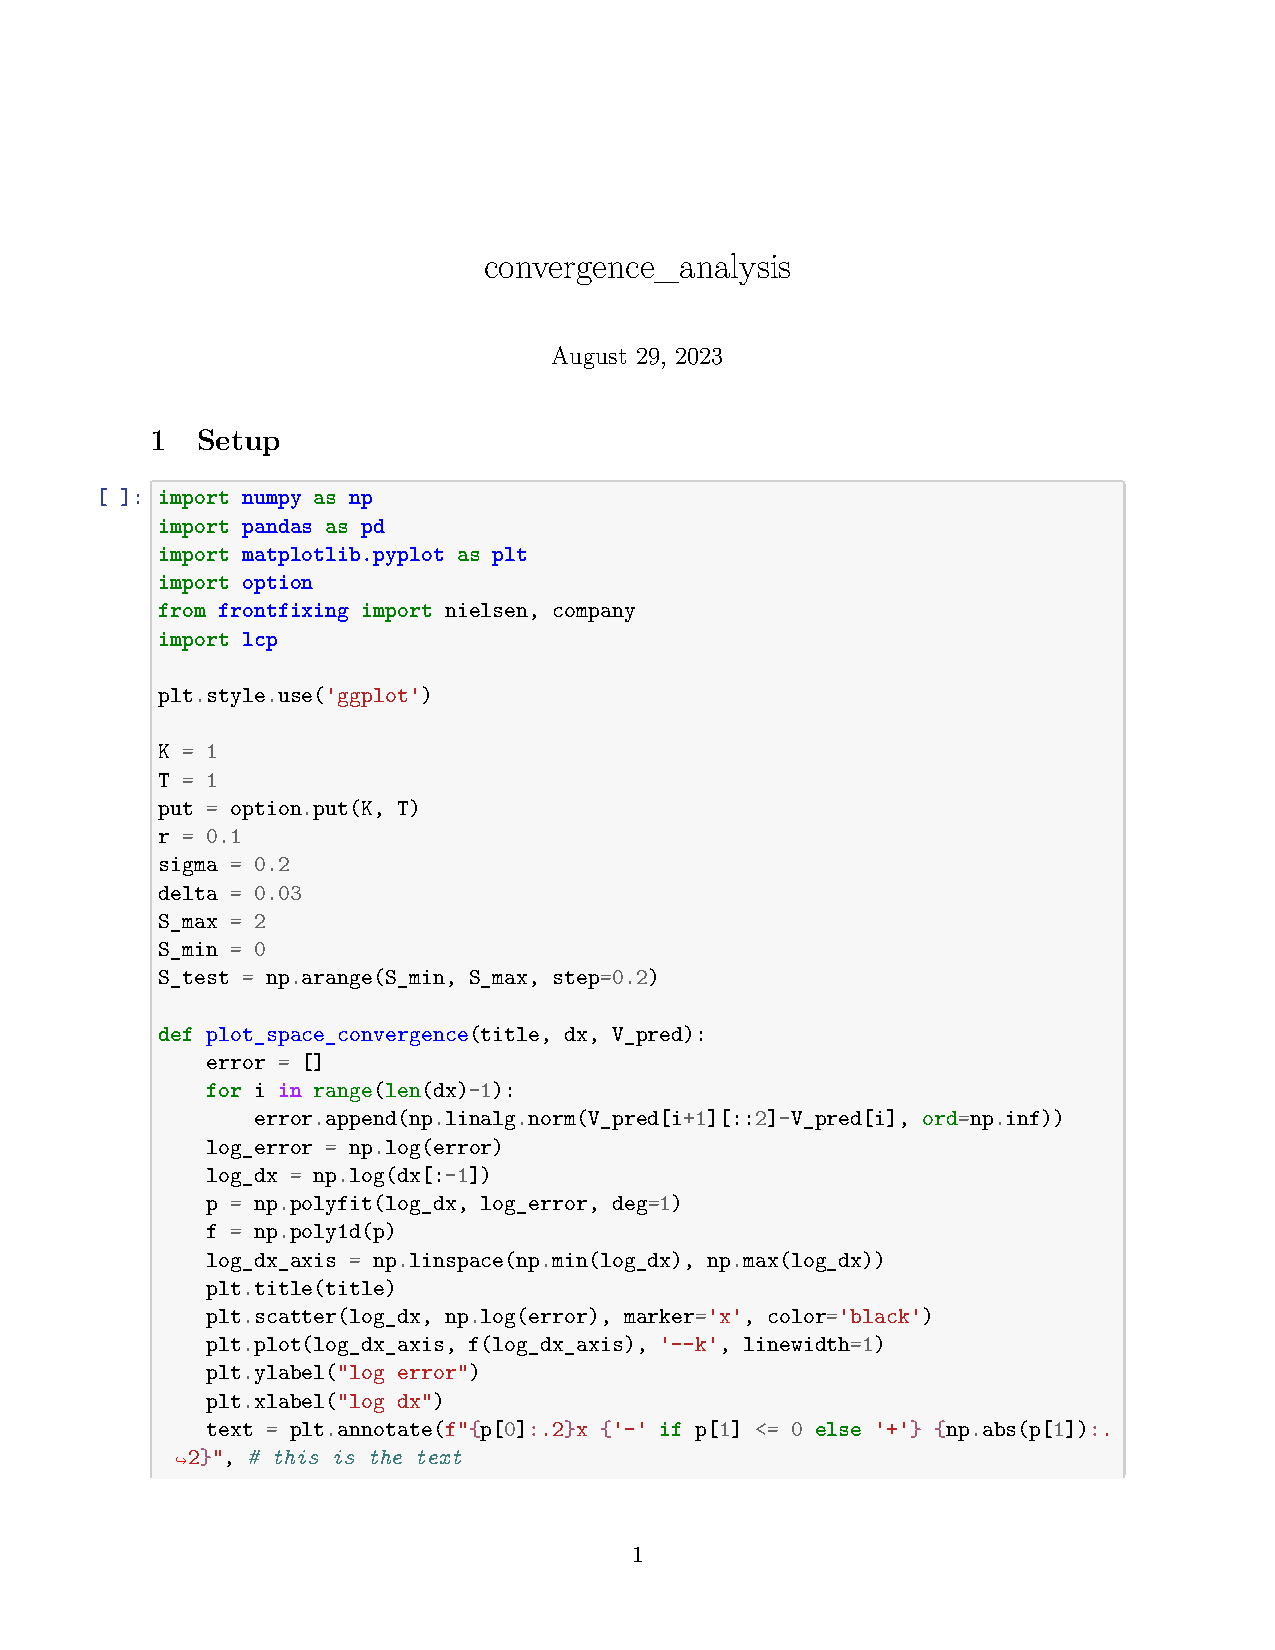
\includegraphics[scale=0.9, clip, trim={2.5cm, 2.5cm 0mm 7cm}]{chapters/appendix/convergence_analysis}
% \includepdf[pages=2-, scale=0.8, pagecommand={\thispagestyle{plain}}, clip,trim=2.5cm 25mm 0mm 0mm]{chapters/appendix/convergence_analysis}
\newpage
\printbibliography

\end{document}
